% SPDX-License-Identifier: Apache-2.0
% Technical reference; embedded didactic figures retain their own attribution.
\documentclass[11pt,a4paper,parskip=half,headings=normal,numbers=noenddot]{scrartcl}
\usepackage{fontspec}
\setmainfont{Latin Modern Roman}
\setsansfont{Latin Modern Sans}
\setmonofont{Latin Modern Mono}[BoldFont=lmmonolt10-bold.otf]
\usepackage[ngerman]{babel}
\usepackage{microtype}
\usepackage[a4paper,top=24mm,bottom=25mm,left=25mm,right=25mm]{geometry}
\usepackage{amsmath,amssymb,mathtools}
\usepackage{graphicx,xcolor,booktabs,longtable,tabularx,array}
\usepackage{enumitem,caption,float,placeins}
\usepackage[most]{tcolorbox}
\usepackage{scrlayer-scrpage}
\usepackage{hyperref,bookmark}
\definecolor{ink}{HTML}{193349}
\definecolor{teal}{HTML}{087F8C}
\definecolor{lightteal}{HTML}{EDF7F7}
\definecolor{warm}{HTML}{A55F16}
\definecolor{muted}{HTML}{536575}
\hypersetup{colorlinks=true,linkcolor=ink,urlcolor=teal,citecolor=teal,
 pdftitle={Die Graph-Definition von SkillPilot},
 pdfauthor={SkillPilot / enpasos},
 pdfsubject={Graphsemantik, rekursive Lerneinheiten, Lernzustand und implizite Beherrschung},
 pdfkeywords={SkillPilot, Skill Graph, Lerneinheit, learning unit, Frontier, Assessment, Curriculum}}
\setkomafont{disposition}{\normalfont\sffamily\bfseries\color{ink}}
\setkomafont{pageheadfoot}{\normalfont\sffamily\small\color{muted}}
\clearpairofpagestyles
\ihead{SkillPilot · Graph-Definition}
\ohead{\headmark}
\automark{section}
\cfoot{\pagemark}
\setlength{\headheight}{17pt}
\setcounter{tocdepth}{2}
\setcounter{secnumdepth}{2}
\setlist{nosep,leftmargin=*,topsep=4pt}
\setlist[description]{style=nextline,leftmargin=0pt,labelwidth=0pt,labelindent=0pt}
\captionsetup{font=small,labelfont=bf,skip=7pt}
% Figures float within their section; generous fractions keep a large figure
% on a page together with running text instead of on a page of its own.
\renewcommand{\topfraction}{.85}
\renewcommand{\bottomfraction}{.7}
\renewcommand{\textfraction}{.1}
\renewcommand{\floatpagefraction}{.8}
\renewcommand{\arraystretch}{1.18}
\newcolumntype{P}[1]{>{\raggedright\arraybackslash}p{#1}}
\renewcommand{\tabularxcolumn}[1]{>{\raggedright\arraybackslash}p{#1}}
\setlength{\emergencystretch}{2em}
\newcommand{\code}[1]{\texttt{#1}}
% Notation: italic capitals are sets and relations, italic lower-case letters
% are arbitrary goals. \nd marks one concrete example node of a figure and
% repeats the figure's own label, so that node A is never read as the set A.
\newcommand{\nd}[1]{\ensuremath{\mathsf{#1}}}
\newcommand{\R}{\mathbb{R}}
\newcommand{\N}{\mathbb{N}}
\newcommand{\Pow}{\mathcal{P}}
\DeclareMathOperator{\Atoms}{Atoms}
\DeclareMathOperator{\Sat}{Sat}
\DeclareMathOperator{\Frontier}{Frontier}
\DeclareMathOperator{\Anc}{Anc}
\DeclareMathOperator{\Desc}{Desc}
\DeclareMathOperator{\ReqAtoms}{RequiredAtoms}
\DeclareMathOperator{\Closure}{Closure}
\DeclareMathOperator{\Pre}{Pre}
\DeclareMathOperator{\Missing}{Missing}
\DeclareMathOperator{\MissingAtoms}{MissingAtoms}
\DeclareMathOperator{\Complete}{Complete}
\DeclareMathOperator{\Own}{Own}
\DeclareMathOperator{\Children}{Children}
\DeclareMathOperator{\Id}{Id}
\DeclareMathOperator{\Title}{Title}
\DeclareMathOperator{\Weight}{Weight}
\DeclareMathOperator{\ShortKey}{ShortKey}
\DeclareMathOperator{\PhaseCompat}{PhaseCompat}
\DeclareMathOperator{\Applicability}{Applicability}
\DeclareMathOperator{\Work}{Work}
\DeclareMathOperator{\Reserve}{Reserve}
\DeclareMathOperator{\Budget}{Budget}
\newcommand{\Score}{\mathit{score}}
\newcommand{\Passed}{\mathit{passed}}
\newcommand{\MaxPoints}{\mathit{maxPoints}}
\newcommand{\PassingPoints}{\mathit{passingPoints}}
\newcommand{\Reff}{R_{\mathrm{eff}}}
\newcommand{\Rat}{R_{\mathrm{at}}}
\newcommand{\Meff}{M_{\mathrm{eff}}}
\newcommand{\srcref}[2]{\href{https://github.com/enpasos/skillpilot/blob/main/#1}{#2}}
\newcommand{\sources}[1]{\par\medskip{\small\noindent\textbf{Quellen.}~#1\par}}
\newtcolorbox{principle}[1]{breakable,colback=lightteal,colframe=teal,
 boxrule=.5pt,arc=1mm,left=3mm,right=3mm,top=2mm,bottom=2mm,
 title={#1},fonttitle=\sffamily\bfseries}
\newcommand{\sourcefig}[4][.48\textheight]{%
 \begin{figure}[htbp]\centering
 \includegraphics[width=\linewidth,height=#1,keepaspectratio]{assets/graph-definition/#2}
\caption[\csname title#4\endcsname]{#3}\label{#4}\end{figure}}
\expandafter\def\csname titlefig:overview\endcsname{Ziele und zwei Kantenarten}
\expandafter\def\csname titlefig:contains\endcsname{Direkte und indirekte Zugehörigkeit}
\expandafter\def\csname titlefig:requires\endcsname{Direkte Voraussetzungen}
\expandafter\def\csname titlefig:inheritance\endcsname{Vom Cluster geerbte Anforderungen}
\expandafter\def\csname titlefig:cycles\endcsname{Effektive Zyklen durch Vererbung}
\expandafter\def\csname titlefig:frontier\endcsname{Die nächsten verfügbaren Ziele}
\expandafter\def\csname titlefig:filters\endcsname{Normalmodus und strikter Modus}


\begin{document}
\begin{titlepage}
\vspace*{6mm}
{\sffamily\large\color{teal} SKILLPILOT · TECHNISCHE REFERENZ\par}
\vspace{7mm}
{\sffamily\bfseries\fontsize{32}{37}\selectfont\color{ink}
Die Graph-Definition\par von SkillPilot\par}
\vspace{7mm}
{\Large Struktur, Mathematik, rekursive Lerneinheiten\par und implizite Beherrschung\par}
\vspace{6mm}
\begin{center}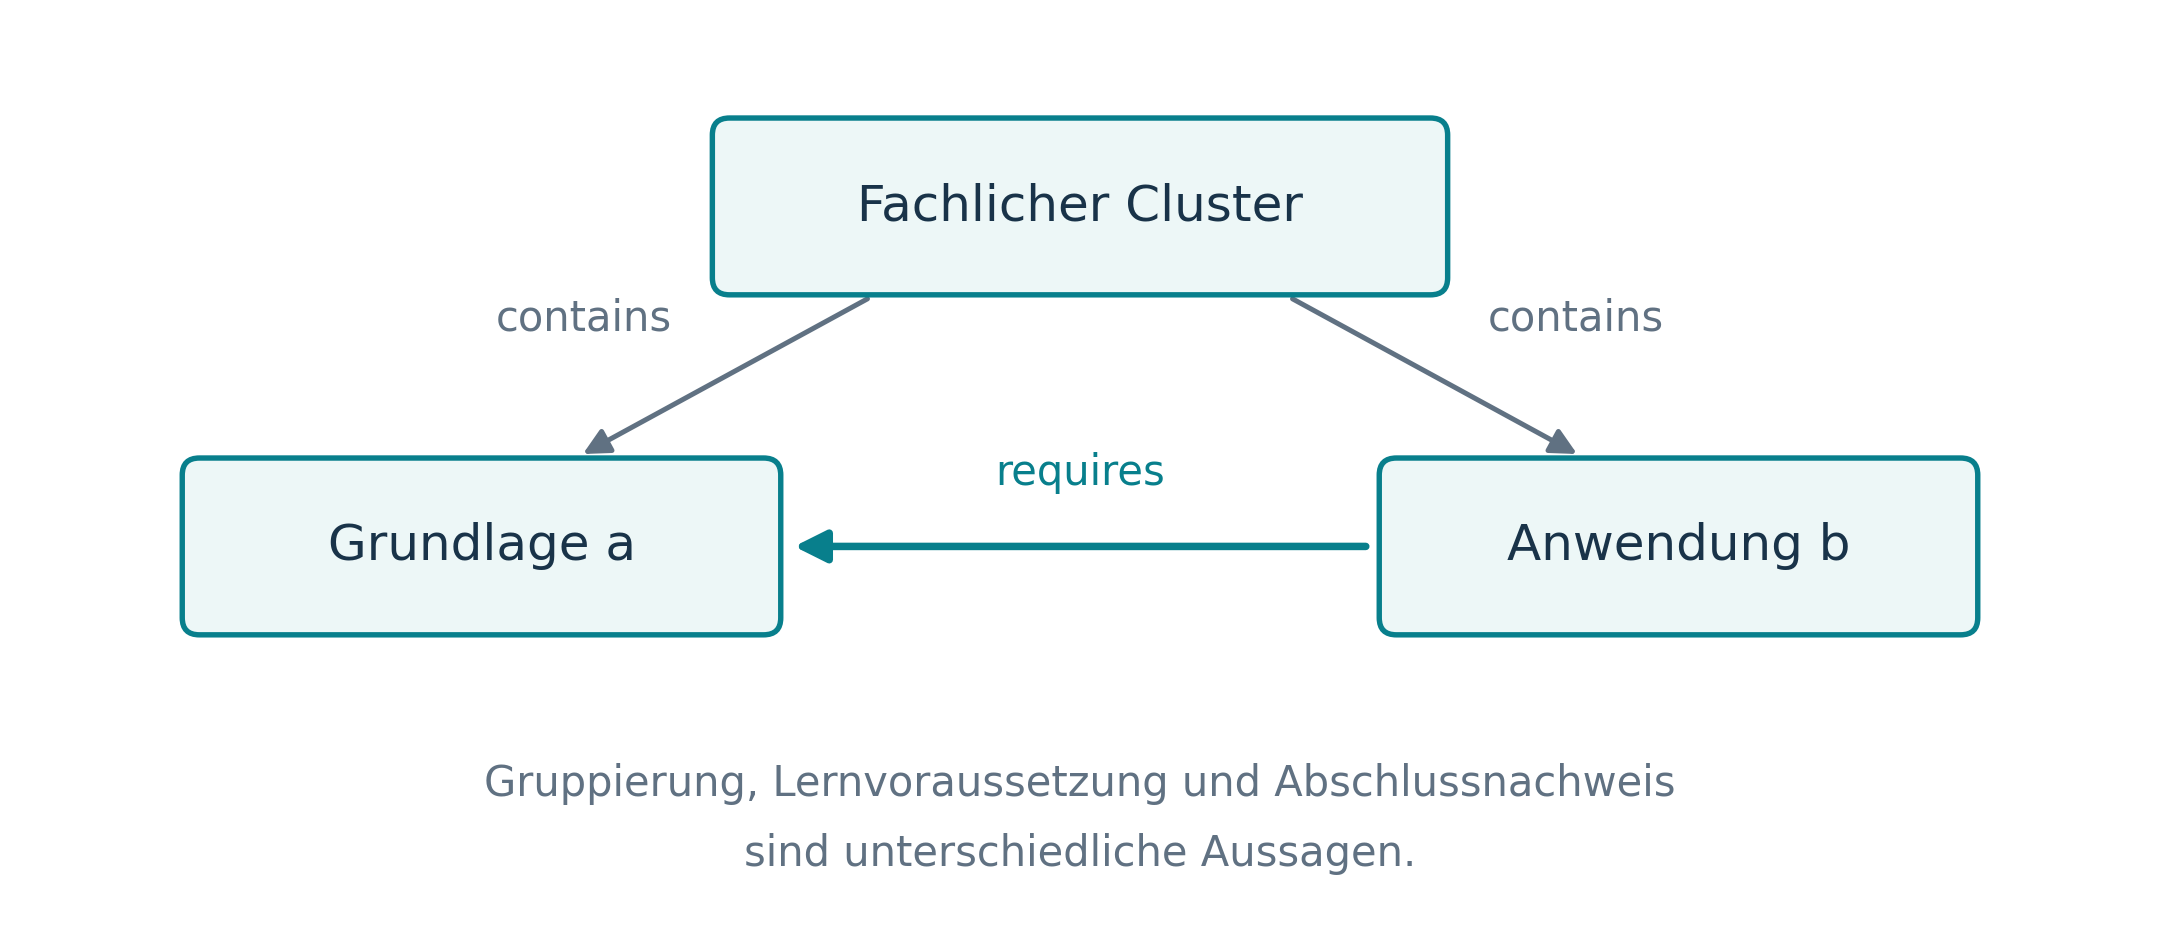
\includegraphics[width=\linewidth,height=.16\textheight,keepaspectratio]{assets/graph-definition/00-title-skill-graph.png}\end{center}
\vfill
\begin{principle}{Geltung dieser Fassung}
Deutsche Gesamtdarstellung, Stand \textbf{9. November 2026}.
SkillPilot beschreibt Lernziele und ihre Beziehungen: \code{contains}
gliedert Ziele, \code{requires} benennt fachliche Voraussetzungen.
Vom kanonischen Zielbestand über das Personal Curriculum bis zum
aktuellen Fokus und den gespeicherten Ergebnissen bleiben die Zielidentitäten
erhalten. \textbf{Lerneinheiten} verbinden ein Lernversprechen mit eigenen
Zielen und Kindeinheiten; Zeitpläne ordnen deren Erwerb verfügbarem
Kalender und Budget zu. Ausdrücklich festgestelltes Verstehen und durch
gültige lokale Prüfungen belegte selbstständige Anwendung zählen beide
zur effektiv beherrschten Zielmenge.

\smallskip\textbf{Geltung und Umsetzung.}
Die atomare Normalform $R\subseteq A\times A$ und die Migrationsreihenfolge
dorthin sind verbindlich.
Anhang~\ref{sec:rule-milestones} ordnet die Regeln ihren Prüfgebieten zu und
grenzt vorhandene Gates ab. Die neue globale Anwendungsanerkennung ist auf
der geprüften Hauptlinie \textbf{noch nicht implementiert};
Anhang~\ref{sec:implementation} beschreibt den Unterschied zum bisherigen
Modell. Der Abschluss einer Lerneinheit wird aus eigenen Pflichten und
Kindern abgeleitet, ohne eine zusätzliche Mastery-Stufe zu speichern.
\end{principle}
\vspace{6mm}
{\small SkillPilot · enpasos -- Enterprise Patterns \& Solutions GmbH\par
Technischer Text und Build-Werkzeuge: Apache-2.0.\par
Didaktische Abbildungen: projektbezogene Inhaltslizenz CC BY 4.0; siehe Anhang.}
\end{titlepage}

\section*{Leserführung und Geltungsbereich}
\markboth{Leserführung}{Leserführung}
\addcontentsline{toc}{section}{Leserführung und Geltungsbereich}
Ein SkillPilot-Graph beschreibt, \emph{was} gelernt werden kann und welche
Voraussetzungen dabei gelten. Darauf bauen vier weitere Aussagen auf, die das
Modell bewusst getrennt hält:
\begin{itemize}
\item \textbf{Curriculare Sichten} bestimmen, welche dieser stabilen Ziele
 für eine Person gelten und wo sie in einem Bildungsgang stehen.
\item Der \textbf{Lernzustand} hält für jedes atomare Ziel fest, ob es
 geschafft ist.
\item \textbf{Lerneinheiten} erklären den fachlichen Zusammenhang vom
 überschaubaren Thema bis zum größeren Fachgebiet. Ihr Abschluss wird
 rekursiv aus Kindern und eigenen Pflichten abgeleitet, nicht pauschal
 gespeichert.
\item Die \textbf{Planung} verteilt Erwerb und Übung auf verfügbare Zeit.
\end{itemize}
Die Ableitung impliziter Beherrschung verbindet ausdrückliche Ergebnisse,
transitive Voraussetzungen und fachlich geprüfte lokale Verträge der
Lerneinheiten. Alle diese Aussagen dürfen sich aufeinander beziehen, aber
nicht stillschweigend gegenseitig ersetzen.

Diese Referenz ist für die deutschsprachige gemeinsame Prüfung und
Weiterentwicklung des Modells bestimmt. Sie behandelt die Graph-Definition
im weiteren Sinne: Identität, Kanten, Vererbung, Gültigkeit, Verfügbarkeit,
Projektion, Zieltypen, Fortschritt, Zeitplanung, Abschluss, Quellen und
Qualitätssicherung. Fachliche Lehrplaninhalte und konkrete Aufgabenbestände
werden nicht vollständig abgedruckt. Die Beispiele sind Veranschaulichungen,
keine als Curriculum freigegebenen Teilgraphen.

\subsection*{Das Modell in sieben Schritten}
Die Schritte nehmen den Gedankengang des Dokuments vorweg. Die englischen
Zielnamen stammen aus dem Mechanik-Beispiel der englischen
Originalabbildungen, erstmals in Abbildung~\ref{fig:overview}.
\begin{enumerate}
\item \textbf{Ziele und zwei Kantenarten.} Ein Lernziel hat eine stabile
 Identität. \code{contains} gliedert: \emph{Kinematics} enthält
 \emph{Velocity}. \code{requires} nennt fachliche Voraussetzungen:
 \emph{Velocity} setzt \emph{Vectors} voraus. Gliederung allein begründet
 keine Voraussetzung (Abschnitte~\ref{sec:core} und~\ref{sec:relations}).
\item \textbf{Atome und Cluster.} Ziele ohne Kinder sind atomar; nur für sie
 wird ein Ergebnis gespeichert. Cluster gliedern. Im Zielzustand verbindet
 jede verfasste Anforderung ein Atom mit einem Atom, und keine ist
 überflüssig. Ältere Anforderungen an oder von Clustern bleiben als
 Übergangsbestand lesbar (Abschnitte~\ref{sec:relations}
 und~\ref{sec:validity}).
\item \textbf{Lernzustand und Frontier.} Je atomarem Ziel gibt es genau ein
 gespeichertes binäres Ergebnis. Als Nächstes verfügbar -- in der
 \emph{Frontier} -- ist ein offenes Atom erst, wenn alle Atome beherrscht
 sind, die es direkt oder über Ketten voraussetzt (Abschnitt~\ref{sec:state}).
\item \textbf{Ausschnitte.} Das Personal Curriculum legt den längerfristigen
 persönlichen Umfang fest, der Fokus den vorübergehenden Arbeitsbereich.
 Abgeleitet wird stets im ganzen Graphen und erst danach eingeschränkt. Der
 Normalmodus prüft die Voraussetzungen innerhalb des Ausschnitts, der
 strikte Modus alle (Abschnitte~\ref{sec:filters}
 bis~\ref{sec:personal-scope}).
\item \textbf{Zieltypen.} Der Zieltyp bestimmt, wann ein Ziel als geschafft
 gilt: ein Inhaltsziel durch festgestelltes Verstehen, ein
 Orientierungsziel durch den abgeschlossenen Einstieg, ein Memorierziel
 durch verifizierten Abruf, ein Prüfungsziel durch die bestandene Prüfung
 (Abschnitt~\ref{sec:goal-types}).
\item \textbf{Lerneinheiten.} Eine Lerneinheit verbindet ein Lernversprechen
 mit eigenen Zielen und Kindeinheiten. Ihr Abschluss wird aus diesen
 Pflichten abgeleitet und nicht zusätzlich gespeichert
 (Abschnitt~\ref{sec:learning-units}).
\item \textbf{Implizite Beherrschung.} Sobald keine offene Prüfung und kein
 offenes Memorierziel einer Lerneinheit ein eigenes Inhaltsziel mehr
 benötigt, gilt dieses Ziel als selbstständig angewandt -- vorausgesetzt,
 der lokale Vertrag der Einheit ist fachlich geprüft und gültig.
 Ausdrücklich festgestelltes Verstehen und so belegte Anwendung bilden
 zusammen die effektiv beherrschte Menge; beide erfüllen spätere
 Voraussetzungen und zählen zum Fortschritt
 (Abschnitt~\ref{sec:assessment}).
\end{enumerate}

\subsection*{Aufbau, Status und Regelkennungen}
Jeder Teil beantwortet eine Leitfrage und hat einen eigenen Status. Die
letzte Spalte nennt die Kennungen, unter denen
Anhang~\ref{sec:rule-milestones} die Regeln des Teils führt, etwa
\code{GD-C07} für eine Regel des formalen Kerns.

\begin{center}\small
\begin{tabularx}{\linewidth}{@{}P{33mm}XP{35mm}P{12mm}@{}}
\toprule
Abschnitte & Leitfrage & Status & Regeln \\
\midrule
\ref{sec:core}--\ref{sec:filters}: Formaler Kern & Was kann gelernt werden,
was setzt es voraus, und was ist als Nächstes verfügbar -- im ganzen Graphen
und in einem Ausschnitt? & Normativer Kern & \code{GD-C}\\
\ref{sec:context-model}--\ref{sec:evidence-context}: Kontext, Sichten,
Zieltypen, Qualität & Wo steht ein Ziel in einem Bildungsgang, was gehört zum
persönlichen Umfang, wann gilt ein Ziel als geschafft, und woher stammt es? &
Angrenzender Vertrag & \code{GD-X}\\
\ref{sec:learning-units}: Lerneinheiten & Welche Ziele bilden ein fachliches
Ganzes, und wann ist es abgeschlossen? & Fachliche Struktur & \code{GD-U}\\
\ref{sec:levels}: Erwerbs- und Zeitplanung & Lässt sich der Erwerb in eine
Reihenfolge und ein Zeitbudget einpassen? & Optionales Profil & \code{GD-P}\\
\ref{sec:assessment}: Implizite Beherrschung & Wann belegt eine bestandene
Prüfung auch die Ziele, auf denen sie aufbaut? & Verbindliches Konzept,
noch nicht implementiert & \code{GD-A}\\
Anhänge \ref{sec:rule-milestones}--\ref{sec:build} & Wie wird welche Regel
geprüft, wo weicht die Implementierung ab, und was bedeuten Begriffe und
Symbole? & Nachschlageteil & \code{GD-D}\\
\bottomrule
\end{tabularx}\end{center}

\begin{center}\small
\begin{tabularx}{\linewidth}{@{}P{35mm}X@{}}
\toprule
Status & Bedeutung in dieser Referenz \\
\midrule
Normativer Kern & Verbindliche mathematische Graphsemantik aus
\code{graph-definition.md}; zusätzliche Profile können strengere Regeln setzen.\\
Angrenzender Vertrag & Semantik von Projektion, Zieltypen, Quellen oder
Lernablauf; der Implementierungsstand ist jeweils gesondert zu prüfen.\\
Fachliche Struktur & Rekursive Lerneinheiten mit Lernversprechen,
eigenen Zielen und abgeleitetem Abschluss; keine behauptete Laufzeitfunktion.\\
Optionales Profil & Zeit- und Budgetplanung sowie bedingte Zugänge zu
Lerneinheiten; harte Sperren und der direkte Prüfungszugang sind dafür noch
nicht entschieden.\\
Noch nicht implementiert & Die neue Anerkennung impliziter Beherrschung ist
verbindlich beschrieben, aber nicht umgesetzt; der bestehende Code folgt
einem abweichenden Bedarfsmodell (Anhang~\ref{sec:implementation}).\\
\bottomrule
\end{tabularx}\end{center}

Wer Curricula verfasst, braucht vor allem die
Abschnitte~\ref{sec:core} bis~\ref{sec:validity}, \ref{sec:goal-types}
und~\ref{sec:evidence-context}. Für die Laufzeitlogik sind die
Abschnitte~\ref{sec:state}, \ref{sec:filters}, \ref{sec:personal-scope}
und~\ref{sec:assessment} maßgeblich, für Qualitätssicherung und Review
zusätzlich die Anhänge~\ref{sec:rule-milestones}
bis~\ref{sec:test-strategy}. Die Abschnitte~\ref{sec:learning-units}
und~\ref{sec:levels} richten sich an alle, die Kurse gliedern und planen.

\subsection*{Lesekonventionen}
\textbf{Verbindlichkeit.} \glqq Muss\grqq, \glqq darf nicht\grqq{} und
\glqq verbindlich\grqq{} kennzeichnen Regeln des Modells.
\glqq Noch nicht implementiert\grqq{} heißt: verbindlich beschrieben, aber
in der Laufzeit nicht umgesetzt. \glqq Optional\grqq{} kennzeichnet ein
Zusatzprofil, \glqq offen\grqq{} oder \glqq noch nicht entschieden\grqq{}
eine bewusst unentschiedene Frage.

\textbf{Schreibweisen.} Kursive Großbuchstaben bezeichnen Mengen und
Relationen ($G$, $A$, $R$, $M$), kursive Kleinbuchstaben beliebige Ziele
($g$, $p$, $a$). Konkrete Beispielknoten einer Abbildung stehen aufrecht und
serifenlos, genau wie im Bild beschriftet: In der Kette
$\nd{Q}\to\nd{B}\to\nd{A}$ ist \nd{A} ein einzelnes Ziel, nicht die Menge
$A$ der atomaren Ziele. Ausgeschriebene Beispielnamen wie \emph{Velocity}
sind kursiv gesetzt. Pfeile zeigen stets in Richtung der Relation, also
vom Cluster zum Kind und vom Ziel zu seiner Voraussetzung.
Schreibmaschinenschrift kennzeichnet Feld- und Bezeichnernamen wie
\code{requires}. Die sieben englisch beschrifteten Abbildungen sind
unveränderte Originale der Quellspezifikation; die Bildunterschriften
erläutern ihre Beschriftungen.

\textbf{Begriffe.} Die folgenden Begriffe werden leicht verwechselt und
deshalb durchgehend in genau dieser Bedeutung verwendet.
Anhang~\ref{sec:glossary} enthält das vollständige Verzeichnis der Begriffe
und Symbole.

\begingroup\small
\begin{longtable}{@{}P{38mm}P{110mm}@{}}
\toprule
Begriffe & Bedeutung in diesem Dokument \\
\midrule\endhead
Anforderung, Voraussetzung & Die Kante $(g,p)\in R$ ist eine
\emph{Anforderung} von $g$; das Ziel $p$ ist eine \emph{Voraussetzung}
von $g$.\\
verfasst, abgeleitet & \emph{Verfasst} sind nur die gespeicherten
\code{contains}- und \code{requires}-Kanten. Geerbte, effektive und atomar
normalisierte Anforderungen sowie Hüllen werden daraus \emph{abgeleitet}.\\
Zielzustand, Übergangsbestand & \emph{Zielzustand} heißt der angestrebte
Zustand der kanonischen Daten: atomare Normalform und transitive
Minimalität. \emph{Übergangsbestand} sind heutige Daten, die noch
Clusteranforderungen enthalten. Der Lernstand eines einzelnen Ziels ist
damit nie gemeint.\\
Mastery, implizite Beherrschung, effektiv beherrscht & \emph{Mastery} ist
das gespeicherte ausdrückliche Ergebnis (Menge $M$). \emph{Implizite
Beherrschung} wird abgeleitet (Menge $I_U$). \emph{Effektiv beherrscht} ist
die Vereinigung beider (Menge $\Meff$).\\
Inhaltsziel, geschütztes Ziel & \emph{Inhaltsziel} heißt das gewöhnliche
fachliche Lernziel; Abbildungen beschriften es mit \glqq gewöhnlich\grqq.
\emph{Geschützt} sind Prüfungs- und Memorierziele: Sie werden nie implizit
bestanden.\\
Cluster, Lerneinheit, Programmeinheit & Ein \emph{Cluster} ist ein Ziel mit
\code{contains}-Kindern. Eine \emph{Lerneinheit} ist eine eigens
autorisierte fachliche Einheit mit Lernversprechen. Eine
\emph{Programmeinheit} ist ein organisatorischer Abschnitt wie Jahrgang
oder Semester.\\
Stufe & Personalisierungsstufe (Level~1--4), Reifegrad der Curriculum-QA
(M0--M7), Planungsstufe eines Zeitplans, Schulstufe und das
Schwierigkeitsfeld \code{level} sind fünf verschiedene Dinge.\\
\bottomrule
\end{longtable}
\addtocounter{table}{-1}% unnumbered table: keep "Tabelle 1" for the first caption
\endgroup

\subsection*{Quellen und Grenzen der Aussagen}
Die fachlichen Verträge im Repository bleiben die maßgeblichen
Einzelquellen. Anhang~\ref{sec:sources} ordnet alle Kapitel diesen Quellen
zu. Anhang~\ref{sec:implementation} stellt die datierten Entscheidungen des
Product Owners zusammen, auf die der Text verweist, und nennt die beim
Erstellen überprüften Implementierungsabweichungen. Mathematische Beispiele,
Bildunterschriften
und Plausibilitätsprüfungen ersetzen weder fachliche Aufgabenreviews noch
Untersuchungen mit Lernenden.

\clearpage
\ohead{Inhalt und Abbildungen}
\tableofcontents
\bigskip
\listoffigures
\clearpage
\ohead{Formaler Kern}
% SPDX-License-Identifier: Apache-2.0
\section{Ziele, Identität und Beziehungen}
\label{sec:core}
Die Abschnitte~\ref{sec:core} bis~\ref{sec:filters} bilden den formalen Kern.
Dieser Abschnitt führt Ziele und die beiden verfassten Kantenarten ein.
Abschnitt~\ref{sec:relations} leitet daraus die Relationen ab, mit denen
gerechnet wird, Abschnitt~\ref{sec:validity} nennt die
Gültigkeitsbedingungen. Abschnitt~\ref{sec:state} beschreibt den Lernzustand
einer Person und Abschnitt~\ref{sec:filters} die Auswertung in einem
Ausschnitt des Graphen.

\subsection{Das Grundobjekt}
Der normative Kern ist ein endlicher gerichteter Graph
\[
 \mathcal G=(G,C,R),\qquad C,R\subseteq G\times G.
\]
$G$ ist die Menge der Lernziele. $C$ steht für \code{contains}: Ein Ziel
enthält ein anderes. $R$ steht für \code{requires}: Ein Ziel setzt ein
anderes voraus. Es gibt genau diese beiden \emph{ausdrücklich verfassten}
Kantenarten im Zielgraphen; nur sie werden von Autorinnen und Autoren
gespeichert. Abgeleitete Relationen, curriculare Platzierungen,
Quellenzuordnungen und Nachweise sind andere Modellschichten.

Ein Paar $(x,y)$ ist gerichtet. Für jede Relation $X$ auf $G$ bezeichnet
\[
 X^{-1}=\{(y,x)\mid(x,y)\in X\}
\]
die Umkehrrelation und $X^+$ die transitive Hülle: $(x,y)\in X^+$ gilt genau
dann, wenn ein gerichteter $X$-Pfad mit mindestens einer Kante von $x$ nach
$y$ führt. Pfade der Länge null zählen nicht. Eine Relation $X$ heißt
\emph{azyklisch}, wenn kein Ziel über einen solchen Pfad zu sich selbst
zurückführt, also $\forall g\in G:(g,g)\notin X^+$ gilt. Ein gerichteter
azyklischer Graph heißt kurz DAG. Die Vereinigung $C\cup R$ ist
\emph{nicht} die Relation, an der pauschal alle DAG-Bedingungen geprüft
werden: Beide Kantenarten haben verschiedene Bedeutungen.
Abschnitt~\ref{sec:validity} nennt die Relationen, die azyklisch sein müssen.

Abbildung~\ref{fig:overview} zeigt beide Kantenarten an einem Beispiel.

\begin{principle}{Die Pfeilrichtung ist Teil der Definition}
$k\xrightarrow{\texttt{contains}}c$: Der Cluster $k$ enthält das Ziel $c$.
\quad
$g\xrightarrow{\texttt{requires}}p$: Das Ziel $g$ setzt $p$ voraus; kurz:
$g$ benötigt $p$.
Eine Lernablaufdarstellung zeigt dagegen $R^{-1}$: von der Voraussetzung
zur darauf aufbauenden Kompetenz. Diese Umkehrung muss beschriftet sein.
\end{principle}

\sourcefig[.42\textheight]{01-skill-graph-overview.png}
{Zwei Beziehungen in einem Graphen. Graue Pfeile gliedern
(\code{contains}), blaue zeigen auf Voraussetzungen (\code{requires}).
\emph{Velocity} benötigt \emph{Vectors};
\emph{Newton's Second Law} benötigt sowohl \emph{Forces} als auch
\emph{Acceleration}. Die Farben der Knoten sind hier keine Lernzustände.
Dieses Mechanik-Beispiel kehrt in den englischen Originalabbildungen bis
Abbildung~\ref{fig:filters} wieder.}
{fig:overview}

\subsection{Attribute und stabile Identität}
Jedes Ziel trägt drei normative Basisattribute. Sie sind totale
Abbildungen, also für jedes Ziel definiert:
\[
 \Id:G\to\mathrm{UUID},\qquad \Title:G\to\Sigma^*,\qquad
 \Weight:G\to\R_{>0}.
\]
$\Id$ ist injektiv: Verschiedene Ziele haben verschiedene IDs.
Die UUID bleibt über Platzierungen, Sprachfassungen und Ansichten hinweg
die kanonische Identität. Kurze Buchstaben in diesem Dokument sind nur
mathematische Bezeichner, keine Aussage zum serialisierten ID-Format.

Zwei weitere Attribute sind Teilabbildungen ($\rightharpoonup$), also nicht
für jedes Ziel definiert. Ein optionaler
$\ShortKey:G\rightharpoonup\Sigma^*$ ist innerhalb einer logischen
Landschaft eindeutig, also innerhalb des zusammengehörigen Zielbestands
eines Curriculums. Mehrere Sprachdateien desselben Ziels
dürfen dasselbe Paar aus ID und ShortKey wiederholen. Die Teilabbildung
$\PhaseCompat:G\rightharpoonup P_{\mathrm{compat}}$ beschreibt dagegen
Kompatibilitäts- oder Anzeigemetadaten, häufig im Feld \code{phase}.
Sie definiert weder kanonische Identität noch die fachliche Lernreihenfolge.
Weitere gebräuchliche Felder ordnet Tabelle~\ref{tab:attributes} ein.

\begin{table}[H]\centering
\begin{tabularx}{\linewidth}{@{}P{29mm}X@{}}
\toprule
Feld & Fachliche Bedeutung außerhalb des minimalen Kerns \\
\midrule
\code{description} & Verständlicher, überprüfbarer Zieltext; typischerweise
\glqq Die lernende Person kann \ldots\grqq. Orientierungsziele haben eine
eigene Semantik (Abschnitt~\ref{sec:goal-types}).\\
\code{area}, \code{tags} & Fachliche Einordnung und Metadaten; ein Tag ersetzt
keine autoritative Entscheidung über Zieltyp oder Geltungsbereich.\\
\code{level} & Schwierigkeit beziehungsweise Anforderungsbereich;
keine fachliche Lerneinheit und keine Personalisierungsstufe.\\
\code{core} & Kernziel versus Erweiterung im jeweiligen Vertrag;
eine Erweiterung kann im gewählten Profil trotzdem verbindliches Ziel sein.\\
\code{weight} & Anteil bei Fortschrittsaggregation; keine Zeitdauer,
keine fachliche Nachweisstärke und keine Bestehenswahrscheinlichkeit.\\
\code{examples} & Referenzen auf Beispiele oder Aufgaben;
Vorhandensein beweist keine Aufgabenqualität oder Kompetenzbeherrschung.\\
\code{resourceLinks} & Bestehendes Referenzfeld unter anderem für eigene
Visualisierungen, offizielle Quellen und Altlinks. Neue optionale externe
Lernmaterialien gehören nach aktuellem Vertrag in getrennte Inhaltspakete.\\
\bottomrule
\end{tabularx}
\caption{Ergänzende Zielattribute und ihre begrenzte Bedeutung.}
\label{tab:attributes}
\end{table}

\subsection{Atomare Ziele und Cluster}
Die \emph{strukturelle} Klassifikation folgt allein aus $C$:
\[
 A=\{g\in G\mid\nexists c\in G:(g,c)\in C\},\qquad K=G\setminus A.
\]
Ein Ziel ohne \code{contains}-Kinder ist \emph{atomar} (ein Atom, ein
Blatt); jedes andere Ziel ist ein \emph{Cluster}. Ein Ziel kann mehrere
Eltern haben: Der kanonische \code{contains}-Graph darf eine Polyhierarchie
sein. Explizite Metadaten zur Klassifikation müssen dazu passen.

Strukturelle Atomarität bedeutet nicht automatisch \emph{semantische}
Atomarität. Ein Blatt mit fünf unabhängigen Teilkompetenzen bleibt formal
ein Blatt, kann jedoch die Qualitätsprüfung verfehlen.

Neben dem Strukturtyp hat ein atomares Ziel einen pädagogischen
\emph{Zieltyp}. Der Normalfall ist das \emph{Inhaltsziel}; Orientierung,
Memorierung und Prüfungen sind besondere pädagogische Arten:
\begin{itemize}
\item Ein \textbf{Inhaltsziel}, das gewöhnliche fachliche Lernziel,
 beschreibt fachliches Verstehen oder Können.
\item Ein \textbf{Orientierungsziel} beschreibt den motivierenden Einstieg.
\item Ein \textbf{Memorierziel} beschreibt den kontrollierten Abruf
 erforderlicher Karten.
\item Ein \textbf{Prüfungsziel} beschreibt eine bewertete Aufgabe mit
 eigenem Bestehenskriterium.
\end{itemize}
Abschnitt~\ref{sec:goal-types} erläutert, wann ein Ziel des jeweiligen Typs
als geschafft gilt. Diese Arten sind keine zusätzlichen Strukturtypen und
keine Programmabschnitte.

\section{Containment, Voraussetzungen und Vererbung}
\label{sec:relations}
Aus den beiden verfassten Kantenarten entstehen die Relationen, mit denen
Verfügbarkeit, Fortschritt und Abschluss berechnet werden.
Tabelle~\ref{tab:relations} gibt die Übersicht; die folgenden
Unterabschnitte definieren ihre Einträge der Reihe nach.

\begin{table}[H]\centering\small
\begin{tabularx}{\linewidth}{@{}P{15mm}P{45mm}X@{}}
\toprule
Symbol & Name & Entstehung und Verwendung \\
\midrule
$C$ & Containment & Verfasste \code{contains}-Kanten. Sie gliedern die Ziele
und bestimmen Atome, Cluster und atomare Basis.\\
$R$ & verfasste (direkte) Anforderungen & Gespeicherte
\code{requires}-Kanten. Im Zielzustand verbinden sie nur Atome.\\
$\Reff$ & effektive Anforderungen & $R$ zusammen mit den Anforderungen,
die ein Ziel von seinen \code{contains}-Vorfahren erbt.\\
$\Rat$ & atomar normalisierte Anforderungen & Jede effektive Voraussetzung
ist durch ihre atomare Basis ersetzt; es bleiben nur Paare von Atomen.\\
$\Rat^+$ & transitive Hülle & Alle über Ketten erreichbaren Voraussetzungen.
Grundlage von Bedarf, Frontier und impliziter Beherrschung.\\
$R_A$ & direkt atomar verfasste Anforderungen & $R\cap(A\times A)$;
Grundlage der Routenprüfung in Abschnitt~\ref{sec:routes}.\\
\bottomrule
\end{tabularx}
\caption{Verfasste und abgeleitete Relationen. Im Zielzustand gilt
$R=R_A=\Reff=\Rat$; abgeleitet wird dann nur noch die Hülle $\Rat^+$.}
\label{tab:relations}
\end{table}

\subsection{Hierarchie und atomare Basis}
Für den endlichen azyklischen Containment-Graphen gelten
\begin{align}
 \Anc(g)&=\{k\in G\mid(k,g)\in C^+\},\\
 \Desc(g)&=\{d\in G\mid(g,d)\in C^+\},\\
 \Atoms(g)&=\begin{cases}\{g\},&g\in A,\\\Desc(g)\cap A,&g\in K.\end{cases}
\end{align}
$\Anc(g)$ enthält die Vorfahren von $g$, $\Desc(g)$ seine Nachfahren und
$\Atoms(g)$ seine \emph{atomare Basis}. Jeder Vorfahr hat Kinder und ist
deshalb ein Cluster. Die Kurzformen $\Anc$ und $\Desc$ entsprechen den
Bezeichnern \code{Ancestors} und \code{Descendants} der Quellspezifikation
und ihrer Bilder.

Jeder Cluster besitzt mindestens ein atomares Blatt: In einem endlichen
azyklischen Graphen endet jeder absteigende Pfad nach endlich vielen
Schritten bei einem Ziel ohne Kinder. Deshalb ist
$\Atoms(g)$ für jedes Ziel nichtleer. Ein Knoten ohne Kinder ist atomar,
kein leerer Cluster. Bei mehreren Pfaden zählt ein Atom in der Menge nur einmal.
Abbildung~\ref{fig:contains} zeigt direkte und indirekte Zugehörigkeit.

\sourcefig{02-contains-relation.png}
{Direkte und indirekte Zugehörigkeit. Der türkis hervorgehobene Pfad besteht
aus zwei vorhandenen \code{contains}-Kanten; er ist keine dritte Kantenart.
\emph{Mechanics} ist deshalb auch Vorfahr von \emph{Velocity}.}
{fig:contains}

\subsection{Direkte Anforderungen sind konjunktiv}
$(g,p)\in R$ bedeutet: $g$ setzt $p$ voraus. Die Kante heißt eine
\emph{Anforderung} von $g$, das Ziel $p$ eine \emph{Voraussetzung} von $g$.
Mehrere ausgehende Kanten bedeuten \emph{alle} Voraussetzungen, keine
Auswahl. Alternativen brauchen einen eigenen Auswahlvertrag außerhalb dieser
Relation. Die Relation $R$ muss azyklisch sein.
Abbildung~\ref{fig:requires} zeigt vier direkte Anforderungen.

Nach der verbindlichen Entscheidung vom 8. November 2026 gilt im
kanonischen Zielzustand
\begin{equation}
 R\subseteq A\times A.
 \label{eq:atomic-target}
\end{equation}
Diese Eigenschaft heißt \emph{atomare Normalform}:
\emph{Alle} verfassten Anforderungen haben atomare Quell- und
Voraussetzungsziele. Auch eine universelle Clusteranforderung, die für
alle Nachfahren eines Clusters gelten soll, ist keine bleibende Ausnahme.
Cluster dienen der Gliederung und abgeleiteten Übersicht.

Daten, die noch Anforderungen von oder an Cluster enthalten, heißen in
diesem Dokument \emph{Übergangsbestand}. Bestehende Clusteranforderungen
behalten im Übergang ihre Lesesemantik:
Eine am Cluster verfasste Anforderung gilt durch Vererbung für alle
Nachfahren; ein Cluster als Voraussetzung wird in seine Atome expandiert
(Abschnitt~\ref{sec:effective}).
Diese Kompatibilität erfüllt noch nicht den kanonischen Zielzustand.

\sourcefig{03-direct-requires.png}
{Direkte Voraussetzungen. Auch der gebogene Pfeil ist eine direkte Kante.
Die Kette von \emph{Acceleration} über \emph{Velocity} zu \emph{Vectors}
ergibt transitive Erreichbarkeit, keine Containment-Vererbung.}
{fig:requires}

\subsection{Effektive Anforderungen}
\label{sec:effective}
Damit auch der Übergangsbestand eindeutig gelesen wird, bereiten drei
Schritte die verfassten Anforderungen auf: erst vererben, dann atomar
expandieren, dann die transitive Hülle bilden. Diese Reihenfolge gilt
überall, wo dieses Dokument mit Voraussetzungen rechnet.

\paragraph{Schritt 1: Vererben.}
Die effektive Relation liest auch bestehende Clusteranforderungen. Sie
entsteht aus eigenen und von Vorfahren geerbten direkten Anforderungen:
\begin{equation}
 (g,p)\in\Reff\iff
 (g,p)\in R\ \lor\ \exists k\in\Anc(g):(k,p)\in R.
 \label{eq:effective}
\end{equation}
Dabei sind
\[
 R_{\mathrm{inherited}}=\Reff\setminus R,\qquad
 \Reff=R\cup R_{\mathrm{inherited}},\qquad
 \Pre_{\mathrm{eff}}(g)=\{p\mid(g,p)\in\Reff\}.
\]
Mehrere Elternpfade addieren Anforderungen als Mengenvereinigung, ohne
Mehrfachzählung. \emph{Vererbung} in \eqref{eq:effective} und
\emph{transitive Hülle} $\Reff^+$ sind verschiedene Operationen:
Vererbung überträgt die Anforderungen der Vorfahren entlang von
\code{contains} auf die Nachfahren; die Hülle folgt Ketten von Anforderungen.
Abbildung~\ref{fig:inheritance} zeigt eine geerbte Anforderung.

\sourcefig{04-effective-requires.png}
{Beispiel aus dem Übergangsbestand: eine vererbte Clusteranforderung.
\emph{Vectors} liegt in diesem Beispiel außerhalb von \emph{Kinematics}.
Wäre es auch darin enthalten, erbte es die Anforderung an sich selbst.
Durchgezogen heißt direkt verfasst, gestrichelt heißt geerbt.}
{fig:inheritance}

\paragraph{Schritt 2: Atomar expandieren.}
Für die Laufzeit wird zuerst auf Atome normalisiert. Jede effektive
Voraussetzung wird durch ihre atomare Basis ersetzt:
\[
 \Rat=\{(a,b)\in A\times A\mid
       \exists p\in G:(a,p)\in\Reff\land b\in\Atoms(p)\}.
\]

\paragraph{Schritt 3: Hülle bilden.}
Die transitive Hülle $\Rat^+$ enthält damit auch Pfade, die
nach der Expansion einer Clusteranforderung weiterführen. Mastery eines
Zwischenziels unterbricht diese Hülle nicht. Auch in
Abschnitt~\ref{sec:assessment} bleibt $\Rat$ die Bezeichnung dieser
normalisierten Relation; $R$ bezeichnet weiterhin die verfassten Kanten.

Abbildung~\ref{fig:atomic-expansion} zeigt die Schritte 2 und 3 an einer
Clusteranforderung. Die externe Grundlage \nd{c} bleibt nach der Expansion
von \nd{K} über \nd{a} erreichbar.
\begin{figure}[htbp]\centering
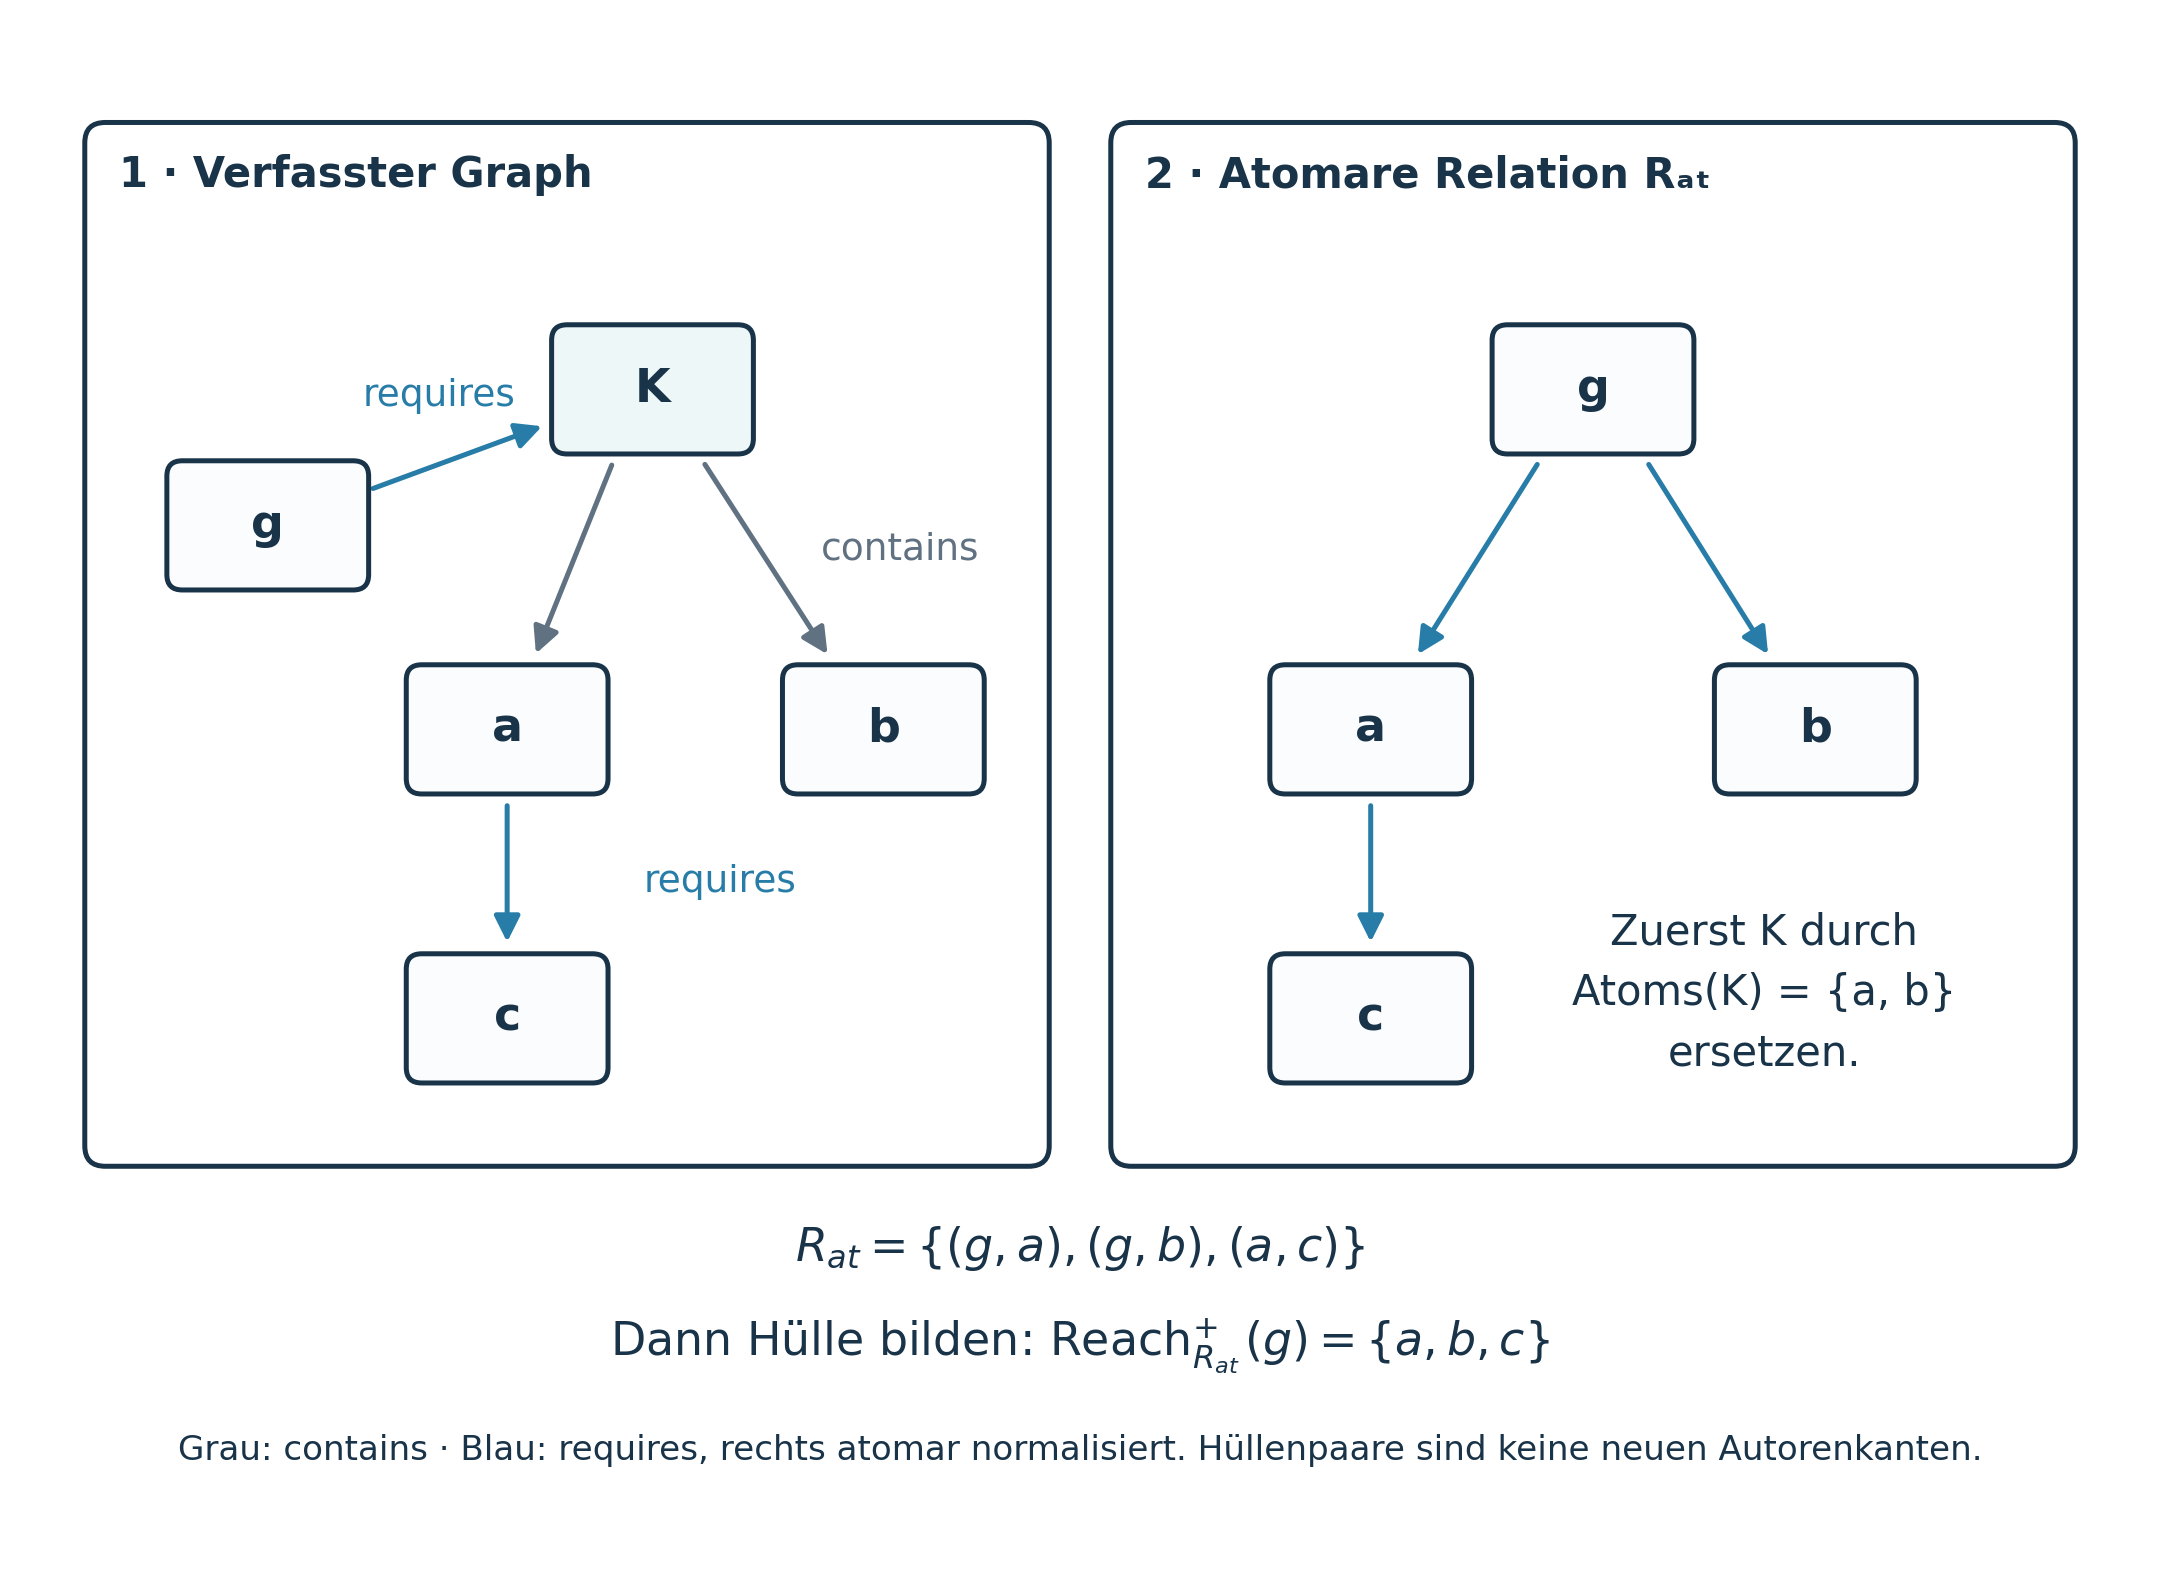
\includegraphics[width=\linewidth]{assets/graph-definition/13-atomic-expansion.png}
\caption[Atomare Expansion vor der Hüllenbildung]{Aus $\nd{g}\to\nd{K}$ und
$\Atoms(\nd{K})=\{\nd{a},\nd{b}\}$ entstehen die atomaren Paare
$(\nd{g},\nd{a})$ und $(\nd{g},\nd{b})$.
Weil außerdem $\nd{a}\to\nd{c}$ gilt, enthält die erst danach gebildete
Hülle auch $(\nd{g},\nd{c})$. Der Beispielknoten \nd{K} ist ein einzelner
Cluster, nicht die Menge $K$ aller Cluster. Die rechte Darstellung zeigt die
abgeleitete atomare Relation, keine zusätzlich verfassten Autorenkanten.}
\label{fig:atomic-expansion}\end{figure}

\paragraph{Der atomare Bedarf eines Ziels.}
Mehrere spätere Formeln fragen dasselbe: Welche Atome setzt ein Ziel
insgesamt voraus? Für ein beliebiges Ziel $g$ seien
\begin{align}
 B(g)&=\bigcup_{p\in\Pre_{\mathrm{eff}}(g)}\Atoms(p),\notag\\
 \ReqAtoms(g)&=B(g)\cup\{b\in A\mid\exists a\in B(g):(a,b)\in\Rat^+\}.
 \label{eq:demand}
\end{align}
$\ReqAtoms(g)$ heißt der \emph{atomare Bedarf} von $g$; die
Quellspezifikation schreibt dafür $D(g)$. Für ein Atom $g$ ist
$\ReqAtoms(g)=\{b\in A\mid(g,b)\in\Rat^+\}$. Für einen Cluster beschreibt
der Bedarf dessen eigene und geerbte Anforderungen, ohne die eigenen Kinder
als zusätzliche Voraussetzungen zu behandeln. Der Bedarf hängt nur vom
Graphen ab, nicht vom Lernzustand. In
Abbildung~\ref{fig:atomic-expansion} ist
$\ReqAtoms(\nd{g})=\{\nd{a},\nd{b},\nd{c}\}$.

Im vollständig atomar verfassten Zielzustand gilt $\Reff=R=\Rat$:
Containment-Vorfahren sind Cluster und tragen dann keine ausgehenden
Anforderungen. Transitive Ketten bleiben als Graphstruktur relevant.

\FloatBarrier
\section{Gültigkeit, Minimalität und Lernbarkeit}
\label{sec:validity}
\subsection{Verbindliche Bedingungen}
Ein vollständiger Graph erfüllt den kanonischen Zielzustand genau dann,
wenn neben den Attribut- und Identitätsbedingungen aus
Abschnitt~\ref{sec:core} auch die atomare Normalform
\eqref{eq:atomic-target}, die Azyklizität und die atomare transitive
Minimalität gelten:
\begin{align}
 &\forall g\in G:\ (g,g)\notin C^+,\quad (g,g)\notin R^+,
                  \quad (g,g)\notin\Reff^+,\quad
                  (g,g)\notin\Rat^+,\label{eq:acyclic}\\
 &\forall(a,b)\in R:\quad
      (a,b)\notin\bigl(R\setminus\{(a,b)\}\bigr)^+.
      \label{eq:atomicmin}
\end{align}
Bedingung~\eqref{eq:acyclic} verlangt, dass keine der vier Relationen ein
Ziel auf sich selbst zurückführt. Bedingung~\eqref{eq:atomicmin} verlangt,
dass keine verfasste Anforderung über die übrigen bereits erreichbar ist.
Identitäten und Referenzen müssen auflösbar sein; unbekannte
Knoten sind keine erfüllten Voraussetzungen.

\paragraph{Zur Azyklizität.}
Die DAG-Bedingung für $R$ folgt bereits aus derjenigen für $\Reff$, weil
$R\subseteq\Reff$. Sie bleibt als verständliche eigenständige
Autorenprüfung aufgeführt. Unabhängig davon bleibt die Azyklizität von $C$
erforderlich. Direkte Azyklizität allein genügt nicht, weil Vererbung einen
Zyklus erzeugen kann (Abbildung~\ref{fig:cycles}). Ebenso bleibt ein
durch atomare Expansion entstehender Selbstzyklus ein Modellfehler,
auch wenn die unexpandierten Kanten azyklisch aussehen.

\sourcefig{05-validity-and-cycles.png}
{Direkte Azyklizität genügt nicht. Der Cluster \nd{A} enthält \nd{B} und
benötigt \nd{X}; daraus folgt die geerbte Kante $\nd{B}\to\nd{X}$. Kommt
$\nd{X}\to\nd{B}$ hinzu, entsteht der effektive Zyklus
$\nd{B}\to\nd{X}\to\nd{B}$. Der Beispielknoten \nd{A} ist hier ein Cluster,
nicht die Menge $A$ der atomaren Ziele.}
{fig:cycles}

\paragraph{Zur transitiven Minimalität.}
In der atomaren Kette $\nd{Q}\to\nd{B}\to\nd{A}$ ist eine zusätzliche Kante
$\nd{Q}\to\nd{A}$ redundant und zu entfernen. Die verbleibende Hülle fordert
\nd{A} weiterhin, auch wenn \nd{B} bereits gemeistert ist.
Transitive Paare werden nicht als zusätzliche Direktkanten gespeichert.
Die verbindliche transitive Minimalität vom 4. November
bleibt bestehen; die Entscheidung vom 8. November legt die atomare
Normalform als Zielzustand und die Migrationsreihenfolge fest.

Die interne Prüfbezeichnung \code{G17} steht hier für die vollständige
atomare Normalform und die vollständige transitive Minimalitätsprüfung
des deklarierten kanonischen Fachbestands. Sie umfasst den nötigen
fachfremden Voraussetzungsbestand und vererbende Vorfahren; ein Teilscan
oder ein einzelnes Routenprofil genügt dafür nicht.

\paragraph{Verbindliche Migrationsreihenfolge.}
Der Weg vom Übergangsbestand zum Zielzustand hat drei Schritte in fester
Reihenfolge. Bei unverändertem $C$ und stabilen Zielidentitäten gilt:
\begin{enumerate}
 \item \textbf{Atomare Anforderungen sichern.} Zuerst die vollständigen,
 im Review geprüften atomaren Anforderungen materialisieren oder erhalten. Die
 bestehende Bedeutung wird mit der Relation $\Rat$ aus
 Abschnitt~\ref{sec:effective} ermittelt: erst vererben, dann Clusterziele
 expandieren, dann die Hülle bilden. Die vollständige Hülle
 bedeutet nicht, sämtliche transitiven Paare als Direktkanten zu verfassen.
 Atomare Kanten dürfen nicht zugunsten ihrer geerbten Clusterentsprechung
 entfernt werden.
 \item \textbf{Clusteranforderungen entfernen.} Danach jede Anforderung mit
 nichtatomarem Quell- oder Voraussetzungsziel erst nach dem Nachweis
 entfernen, dass die verfassten atomaren Beziehungen ihren vollständigen
 atomaren Bedarf abdecken. Im Zielzustand bleiben keine solchen
 Clusterkanten, auch keine universellen.
 \item \textbf{Transitiv reduzieren.} Erst anschließend die atomare Relation
 transitiv reduzieren und dabei ihre vollständige Voraussetzungshülle
 erhalten.
\end{enumerate}
Der Nachweis muss für den gesamten Übergang insbesondere ergeben:
\[
 (\Rat^{\mathrm{vorher}})^+
 = (\Rat^{\mathrm{nachher}})^+
 = R_{\mathrm{nachher}}^+,\qquad
 R_{\mathrm{nachher}}\subseteq A\times A.
\]
Die atomare Voraussetzungshülle bleibt also gleich, und nach der Migration
erzeugen die verfassten Kanten sie allein. Zusätzlich sind die relevanten
Scope-, Anwendbarkeits-, Zielmengen-, Frontier-, Abschluss- und
Mastery-Verträge zu erhalten. Hüllengleichheit
allein beweist diese weiteren Verträge nicht; dazu gehören direkt atomare
Routen und ausdrücklich verfasste Projektionsrollen. Rohe Erreichbarkeit
zwischen nichtatomaren Zielknoten darf sich beim Entfernen der Clusterkanten
ändern. Die Migration erfindet weder automatisch fachliche Abhängigkeiten
noch Rollen und schreibt keine Lernergebnisse. Widersprüchliche Altansprüche
brauchen eine gesonderte fachliche Klärung.

\paragraph{Diagnosen im Übergangsbestand sind keine Löschanweisung.}
Zwei ältere Prüfungen bleiben als Diagnose nützlich. Keine von ihnen
erlaubt, eine atomare Kante zu löschen, solange eine Clusteranforderung
denselben Bedarf noch trägt.

Die frühere \emph{lokale Minimalitätsbedingung} lautet
\begin{equation}
 (g,p)\in R\Longrightarrow
 \nexists k\in\Anc(g):(k,p)\in R.
 \label{eq:localmin}
\end{equation}
Sie zeigt direkte Dubletten geerbter Anforderungen, darf aber keine atomare
Kante zugunsten einer Clusterkante beseitigen. Tragen ein atomares $q$ und sein
Cluster-Vorfahr $k$ beide die Anforderung an das atomare $p$, bleibt $q\to p$
bei der Atomarisierung erhalten. Nach vollständiger atomarer Abdeckung wird
$k\to p$ entfernt. Im Zielzustand gilt \eqref{eq:localmin} automatisch,
weil Cluster keine ausgehenden Anforderungen mehr tragen.

Der bisher unter \code{G17} verwendete \emph{Entfernungstest} ist ebenfalls
eine Diagnose des Übergangsbestands: Er bildet für jede verfasste Kante
$e=(g,p)$ die Relation $R'=R\setminus\{e\}$ und berechnet
$R_{\mathrm{eff}}'$ mit unverändertem $C$ neu. Er diagnostiziert
Redundanz durch $(g,p)\in(R_{\mathrm{eff}}')^+$.
Abbildung~\ref{fig:inherited-redundancy} zeigt diesen mathematisch korrekten
Befund im Übergangsbestand und zugleich den Gegenfall zur falschen
Löschpräferenz:
Der alternative Pfad hängt noch von einer Clusteranforderung ab.
\begin{figure}[htbp]\centering
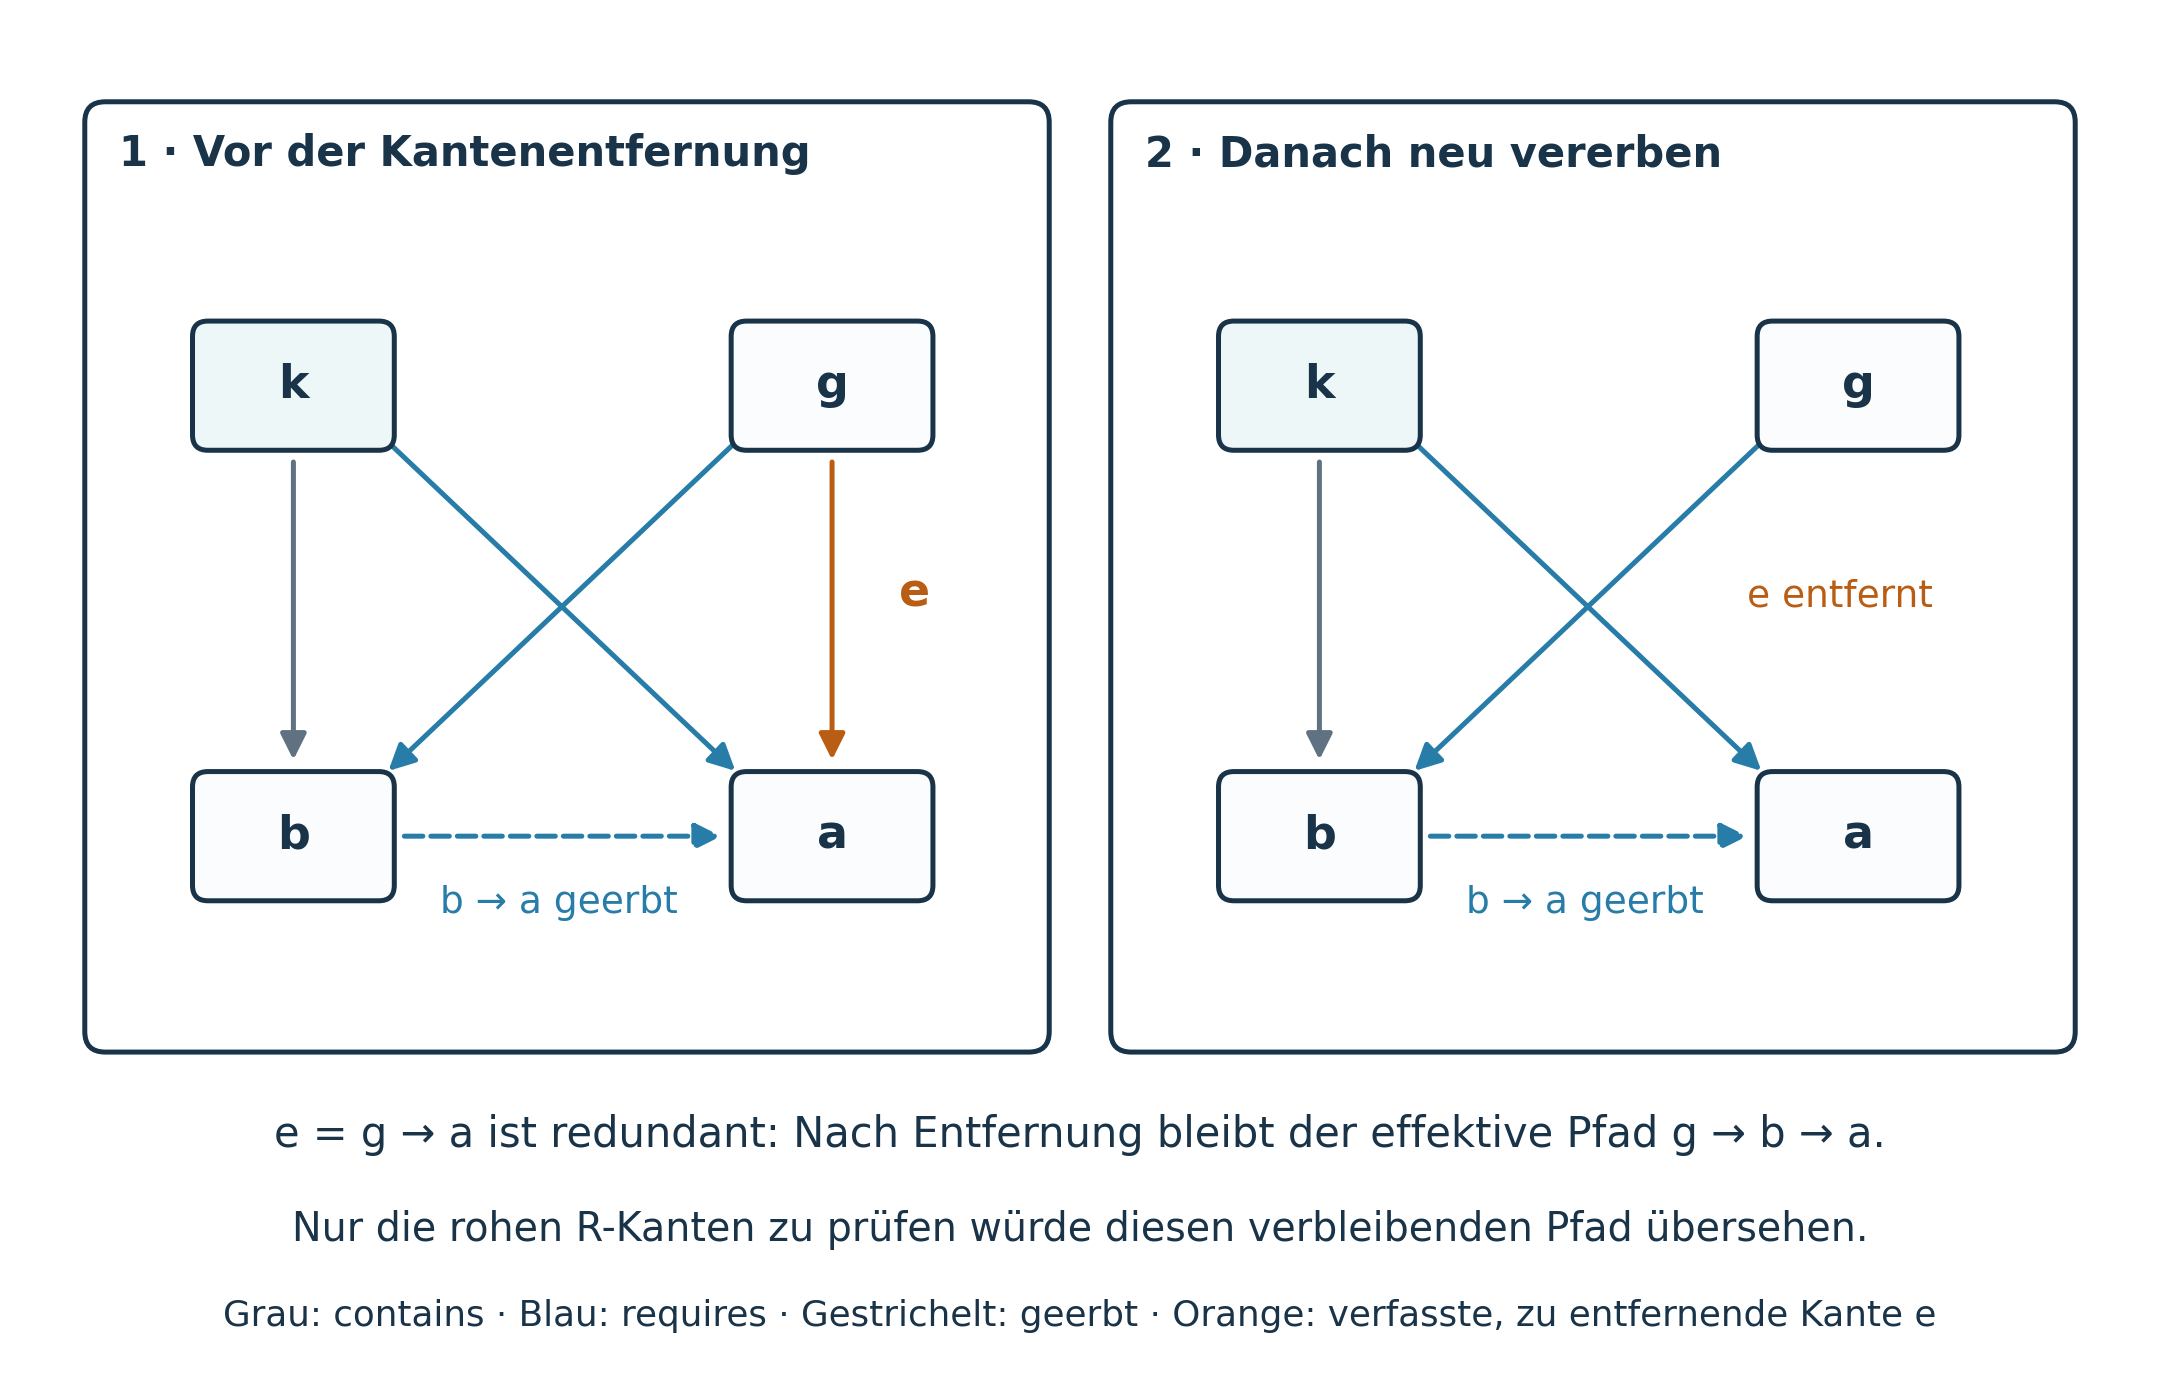
\includegraphics[width=\linewidth]{assets/graph-definition/14-inherited-redundancy.png}
\caption[Übergangsdiagnose: geerbte Redundanz]{Der Cluster \nd{k} enthält
\nd{b} und benötigt \nd{a}; deshalb erbt \nd{b} die Anforderung
$\nd{b}\to\nd{a}$. Entfernt man die verfasste Kante
$\nd{e}=(\nd{g},\nd{a})$, bleibt nach erneuter Vererbung der effektive Pfad
$\nd{g}\to\nd{b}\to\nd{a}$. Das ist eine Redundanzdiagnose des
Übergangsgraphen, kein Auftrag, \nd{e} zugunsten von $\nd{k}\to\nd{a}$ zu
löschen. Zuerst ist die vollständige atomare Abdeckung von
$\nd{k}\to\nd{a}$ zu materialisieren, dann die Clusterkante zu
entfernen; erst danach entscheidet ein vollständig atomarer Ersatzpfad über
die Reduktion von \nd{e}. Nur die geerbte Kante ist gestrichelt.}
\label{fig:inherited-redundancy}\end{figure}

\paragraph{Was die heutigen Prüfungen belegen.}
Der heutige Entfernungsauditor prüft noch das alte effektive Kriterium auf
Zielknoten; sein Bestehen beweist die neue Migrationspriorität nicht.
Erst im atomaren Zielzustand entspricht dieses Kriterium der
Minimalität aus \eqref{eq:atomicmin}. Die Norm ist keine Behauptung bereits
vollständiger Datenmigration oder CI-Durchsetzung.

Zwei Regelfamilien prüfen heute Teile des Zielzustands: das
\emph{Curriculum-Quality-Review} (CQR) und die \emph{graph-validation
rollout rules} (GVR). Die Prüfung direkt atomarer Fachrouten heißt
\code{CQR-102}; die harte vollständige Routenprüfung der Mathematikprofile
Sek~I und Sek~II heißt \code{GVR-012}.
Beide verlangen bereits in ihrem jeweiligen Scope, also ihrem benannten
Prüfumfang, direkt atomare Routen; geerbte Clusterpfade liefern dort keinen
Ersatz. Die Codelegende steht in Anhang~\ref{sec:rule-code-legend}.

\subsection{Zusatzprofile und Gegenbeispiele}
Ein Baumprofil kann höchstens einen Elternknoten fordern:
\[
 \forall c\in G:\quad
 \bigl|\{k\in G\mid(k,c)\in C\}\bigr|\leq1.
\]
Dies ist keine Grundbedingung der Polyhierarchie. Ebenso sind Anforderungen
an eigene Vorfahren unerwünscht und in bestimmten Validatorprofilen
verboten. Anforderungen an eigene Nachfahren erzeugen durch Vererbung sogar
eine effektive Selbstabhängigkeit und scheitern bereits am DAG-Vertrag.

\begin{principle}{Ein DAG ist noch kein Beweis der Lernbarkeit}
Als Gegenbeispiel aus dem Übergangsbestand seien $G=\{k,a\}$,
$C=\{(k,a)\}$ und $R=\{(a,k)\}$: Der Cluster $k$ enthält das Atom $a$, und
$a$ setzt $k$ voraus.
Die direkten und effektiven Relationen sind azyklisch und minimal.
Aber $\Atoms(k)=\{a\}$: Um $a$ zu beginnen, müsste $a$ schon erfüllt sein.
Die globale Frontier aus leerem Lernzustand ist leer.
Die Clusteranforderung verfehlt bereits die atomare Normalform. Außerdem
enthält die vollständig atomar normalisierte Relation die Selbstabhängigkeit
$(a,a)$ und verletzt damit die Azyklizität. Ein Abschlusszeuge
(Abschnitt~\ref{sec:witness}) würde denselben Fehler sichtbar machen.
\end{principle}

Deshalb müssen drei Aussagen getrennt bleiben:
\begin{enumerate}
\item Der Grundgraph ist gültig.
\item Die gewählte Projektion ist gültig.
\item Die Zielmenge ist aus einem deklarierten Eintrittszustand vollständig
 erlernbar.
\end{enumerate}
Ein grüner einzelner Validator beweist nicht automatisch alle drei Aussagen.

\subsection{Didaktische Routen von Orientierung zu Autonomie}
\label{sec:routes}
Eine didaktische Route führt vom motivierenden Einstieg über das fachliche
Lernen zur selbstständigen Leistung. Seien dazu $O\subseteq A$ die
Orientierungsanker (Motivationsanker), $Z\subseteq A$ die terminalen
Autonomieziele, also die Endziele selbstständiger Leistung, und
$E_{\mathrm{route}}\subseteq A$ explizit ausgenommene Unterstützungsziele.
Die direkte atomare Relation sei
% O and Z avoid collisions with mastery and target sets.
$R_A=R\cap(A\times A)$. Ohne Ausnahmeprofil gilt
$E_{\mathrm{route}}=\varnothing$; Ausnahmen benötigen einen dokumentierten,
maschinenlesbaren Auswahlvertrag. Ein Atom $a\in A\setminus E_{\mathrm{route}}$
ist \emph{routenabgedeckt}, wenn
\begin{equation}
 \begin{split}
 \exists o\in O,\ z\in Z:\quad
 &(a=o\ \lor\ (o,a)\in(R_A^{-1})^+)\\[-1mm]
 {}\land\;&(a=z\ \lor\ (a,z)\in(R_A^{-1})^+).
 \end{split}
\end{equation}
In Worten: Das Atom liegt auf mindestens einem Lernweg, der bei einem
Orientierungsanker beginnt und bei einem terminalen Autonomieziel endet.
Der Lernweg folgt $R_A^{-1}$, also der Lernablaufrichtung von der
Voraussetzung zum darauf aufbauenden Ziel.

Die Mengen $O$ und $Z$ heißen in Abschnitt 8.5 der englischen
Quellspezifikation $M$ und $T$. Die abweichenden Buchstaben vermeiden hier
Verwechslungen mit der Mastery-Menge $M$ sowie den Zielmengen $T(U)$ und
$T_\pi$.
Die Beschränkung auf $R_A$ verhindert, dass ein Cluster als versteckter
Zwischenknoten einen atomaren Routennachweis liefert. Diese Formel ist
ein Strukturkriterium, kein Beweis didaktischer Angemessenheit.

Konkrete Routenprofile schränken zusätzlich die Schulstufe, erlaubte
Zieltypen und die Reihenfolge ein: Orientierung am Einstieg,
fachliches Lernen, bei Bedarf Unterstützung durch Memorierziele und eine
selbstständige Leistung am Ende. Memorierziele werden dadurch nicht überall
Pflicht.
Die Profilregeln prüfen unterschiedliche Aussagen: vollständige Routen
über effektive Voraussetzungen (\code{CQR-101}), direkt atomare Routen
(\code{CQR-102}) und das Fehlen von \code{requires} an den selektierten
Clustern (\code{CQR-103}). In den benannten Mathematikprofilen erzwingt
\code{GVR-012} die vollständige direkt atomare Route; \code{GVR-013}
prüft für die ausgewählten lokalen atomaren Ziele, die keine Memorierziele
sind, dass ihre direkten lokalen Voraussetzungen atomare Ziele sind. Diese
Profilprüfungen sind kein globaler Nachweis der atomaren Normalform für alle
Fächer.

Eine Übersicht zwischen Clustern kann aus atomaren Routen abgeleitet werden.
Beispielsweise bedeutet eine existenzielle Zusammenfassung $k_2\to k_1$:
\[
 \exists a\in\Atoms(k_2),\ b\in\Atoms(k_1):(a,b)\in R_A^+.
\]
Eine prozentuale Abdeckung braucht darüber hinaus einen erklärten Nenner.
Solche Übersichten erzeugen keine neuen direkten Clusteranforderungen.

\FloatBarrier
\section{Lernzustand, Erfüllung und Fortschritt}
\label{sec:state}
Die bisherigen Abschnitte beschreiben den Graphen ohne lernende Person.
Dieser Abschnitt fügt ihren Lernzustand hinzu: was gespeichert wird, was
daraus als effektiv beherrscht gilt, welche Ziele als Nächstes verfügbar
sind und wie Fortschritt gezählt wird.

\subsection{Erfüllung statt Rückschluss auf Voraussetzungen}
\paragraph{Ausdrückliche Ergebnisse.}
Es gibt genau einen gespeicherten binären Zustand $m:A\to\{0,1\}$,
mit $M=\{a\in A\mid m(a)=1\}$. $M$ ist die Menge der ausdrücklichen Erfolge,
kurz: die ausdrückliche Mastery. Ein ausdrücklicher Erfolg an einem
Inhaltsziel belegt zielgerecht geprüftes Verstehen. Orientierung,
Memorierung und Prüfungen verwenden ihren jeweils eigenen Abschlussvertrag
(Abschnitt~\ref{sec:goal-types}). Keine Teilbewertung
bildet einen dritten Mastery-Zustand.

\paragraph{Implizite Beherrschung im Vorgriff.}
Die Abschnitte~\ref{sec:learning-units} und~\ref{sec:assessment} führen
Lerneinheiten und die Ableitung impliziter Beherrschung ein. Hier genügt
ihr Ergebnis:
Für jede Lerneinheit $U$ mit einem für diese Person dauerhaft
gültigen lokalen Vertrag wird die implizite Menge $I_U\subseteq A$ abgeleitet.
Der Vertrag bindet die eigenen Erwerbsziele, ihre Revision und die fachlich
geprüfte Bedeutung der zugehörigen Prüfungen.
Bei Inhaltszielen belegt $I_U$ selbstständige Anwendung.
Anschaulich kann eine bestandene Prüfung zu linearen Funktionen die
Anwendung der eigenen Inhaltsziele von $U$ belegen, obwohl diese
nicht einzeln abgehakt wurden. Eine unabhängige Kartenpflicht oder eine
andere Kindeinheit kann noch offen sein; der vollständige Abschluss der
Einheit ist keine Voraussetzung dieser Anerkennung. Ein abgeleiteter
Orientierungsmarker behält ausschließlich die Bedeutung eines erledigten
Einstiegs; er behauptet weder Fachkompetenz noch eine erfolgte
Motivationsinteraktion.

\paragraph{Effektiv beherrschte Menge.}
Die effektive globale Menge lautet
\[
 \Meff=M\cup\bigcup_{U\in\mathcal U_{\mathrm{valid}}}I_U.
\]
Dabei enthält $\mathcal U_{\mathrm{valid}}$ die personen- und
revisionsgebundenen, dauerhaft anwendbaren autoritativen lokalen Verträge,
nicht nur die gerade sichtbaren Einheiten oder die neuesten Inhaltsfassungen.
Die beiden Begründungsarten sind in ihrem effektiven Ergebnis gleichwertig:
Sie erfüllen künftige Voraussetzungen, zählen zum IST und bleiben bei
Fokus- oder Planwechsel wirksam. $I_U$ erzeugt keinen synthetischen
Mastery-Datensatz. Abschnitt~\ref{sec:assessment} definiert die Ableitung
und die fachlichen Voraussetzungen des Vertrags.

Alle folgenden Formeln verwenden $\Meff$. Die englische Quellspezifikation
und ihre Abbildungen schreiben $M_A$ für die ausdrückliche Menge $M$. In
den Beispielen der Abbildungen~\ref{fig:frontier} und~\ref{fig:filters}
gibt es keine implizite Beherrschung; dort ist $\Meff=M$.

\paragraph{Erfüllung.}
Ein Ziel $g$, ob Atom oder Cluster, ist \emph{erfüllt}, wenn seine gesamte
atomare Basis effektiv beherrscht ist:
\begin{equation}
 \Sat(g,\Meff)\iff
 \Atoms(g)\ne\varnothing\ \land\ \Atoms(g)\subseteq\Meff.
 \label{eq:sat}
\end{equation}
Die Erfüllung wirkt nur vorwärts. Ein bloß gemeistertes abhängiges
Inhaltsziel beweist seine Voraussetzungen nicht. Nur ein gültiger lokaler
Vertrag trägt die zusätzliche Ableitung. Clusterfortschritt schreibt
niemals Ergebnisse seiner Kinder.

\subsection{Globale Frontier}
Die \emph{Frontier} ist die Menge der nächsten verfügbaren atomaren Ziele:
\begin{equation}
 \Frontier(\Meff)=\left\{g\in A\setminus\Meff\;\middle|\;
 \forall p\in A:\ (g,p)\in\Rat^+\Rightarrow p\in\Meff\right\}.
 \label{eq:frontier}
\end{equation}
Ein Atom gehört also zur Frontier, wenn es selbst noch offen ist und sein
gesamter atomarer Bedarf effektiv beherrscht ist:
$\ReqAtoms(g)\subseteq\Meff$.
Die Frontier fordert die transitiven effektiven atomaren Voraussetzungen.
Ein gemeistertes Zwischenziel unterbricht diese Prüfung nicht. Ein teilweise
bearbeitetes Ziel ist nicht schon deshalb erfüllt. Ein Cluster als
Voraussetzung wird über seine atomare Basis geprüft.

Für die Navigation lässt sich zusätzlich eine Clusterverfügbarkeit
ableiten. Sie verwendet den atomaren Bedarf $\ReqAtoms(k)$ des Clusters aus
\eqref{eq:demand}, also seine eigenen und geerbten Anforderungen, atomar
expandiert und transitiv fortgesetzt:
\begin{equation}
 \Frontier_K(\Meff)=\{k\in K\mid\neg\Sat(k,\Meff),\ \ReqAtoms(k)\subseteq\Meff\}.
\end{equation}
Sie ersetzt die atomare Lernfrontier nicht. Eine Oberfläche kann darüber
hinaus verbindliche Zugangs- und Auswahlregeln anwenden, etwa den
Orientierungseinstieg. Die mathematische Frontier ist deshalb nicht
automatisch identisch mit jedem angezeigten UI-Menü.
Abbildung~\ref{fig:frontier} zeigt die Frontier des Beispiels.

\sourcefig{06-available-next-goals.png}
{Mit $\Meff=\{\text{Vectors},\text{Forces}\}$ ist nur \emph{Velocity} als
nächstes verfügbar. \emph{Acceleration} wartet auf \emph{Velocity};
\emph{Newton's Second Law} zusätzlich auf \emph{Acceleration}.
Die Cluster sind keine direkt auszuwählenden atomaren Lernschritte. Die
Bildbeschriftung $M_A$ bezeichnet die ausdrückliche Menge $M$, die hier mit
$\Meff$ übereinstimmt.}
{fig:frontier}

\subsection{Aggregation ohne Mehrfachzählung}
Sei $S\subseteq A$ eine fest benannte Menge von Zielatomen und
$w(a)>0$ das Fortschrittsgewicht des Atoms $a$. Der gewichtete
Gesamtfortschritt ist der Gewichtsanteil der effektiv beherrschten Atome:
\begin{equation}
 P(S)=\frac{\sum_{a\in S\cap\Meff}w(a)}{\sum_{a\in S}w(a)}\qquad(S\ne\varnothing).
\end{equation}
Jedes Atom trägt mit seinem effektiven binären Ergebnis bei: ganz oder gar
nicht. Für eine leere Zielmenge gibt es keinen solchen Quotienten; die
Anzeige braucht \glqq keine Ziele im gewählten Umfang\grqq{} statt
erfundener 100\,\%.
Für mehrere Cluster wird $S$ als Vereinigung ihrer Zielatome gebildet.
Cluster und Kinder dürfen nicht zusätzlich gemeinsam gezählt werden.
Ein Fortschritt von beispielsweise 50\,\% bezeichnet einen Anteil
geschaffter Ziele im Umfang, keine halbe Beherrschung eines einzelnen Ziels.

Davon zu unterscheiden ist die segmentierte Erledigungsanzeige im
Lernzielbaum:
Sie kann ausdrücklich gespeicherte und implizit abgeleitete Beiträge
getrennt ausweisen. Beide zählen in $P(S)$; ein vollständig gefüllter
Gesamtbalken bedeutet $P(S)=1$. Eine gesonderte Zahl nur für ausdrückliche
Ergebnisse muss ihren abweichenden Zähler benennen.

Bei der Konvention $w(a)=1$ entspricht das Clustergewicht der Zahl seiner
eindeutigen atomaren Nachfahren. Das ist eine zulässige konkrete
Autorenkonvention, keine Forderung gleicher Gewichte für jede Domäne.
Kern- und Erweiterungsanteile können getrennt ausgewiesen werden; der
verbindliche Zielumfang des Personal Curriculum entscheidet darüber, was zum
Abschluss gehört. Eine aggregierte Zahl ist weder eine kalibrierte
Wahrscheinlichkeit noch eine Schulnote. Ein Notenmodell bräuchte eine
gesonderte, begründete Abbildung.

\FloatBarrier
\section{Filter, Fokus und globale Diagnose}
\label{sec:filters}
Bisher wurde der gesamte Graph ausgewertet. Eine Person arbeitet aber in
einem Ausschnitt: längerfristig in ihrem Personal Curriculum
(Personalisierungsstufe~2, kurz Level~2), vorübergehend in einem Fokus
(Level~3). Dieser Abschnitt beschreibt jeden solchen Ausschnitt als Filter
und legt die Reihenfolge fest: erst im ganzen Graphen ableiten, dann
einschränken. Die Abschnitte~\ref{sec:context-model}
und~\ref{sec:personal-scope} führen Personal Curriculum, Kompositionssicht
und Projektionsrollen ausführlich ein.

\subsection{Filter als Prädikat und kompilierte Anwendbarkeit}
Ein Filter ist zunächst nur ein Prädikat $F:G\to\{0,1\}$ mit der Menge
$G_F=\{g\mid F(g)=1\}$ der ausgewählten Ziele. Ein Filter kann aus
dimensionaler \emph{Anwendbarkeit} (\code{applicability}) berechnet werden,
etwa nach Bundesland, Schulstufe oder Kursprofil. Dafür sei $D$
die Dimensionsmenge und $V_d$ das Vokabular von Dimension $d$. Eine
formal typisierte Menge partieller Zuordnungen ist
\[
 \mathcal V_D=\bigsqcup_{J\subseteq D}\prod_{d\in J}\Pow(V_d),\qquad
 \Applicability:G\rightharpoonup\mathcal V_D.
\]
Eine Anwendbarkeitsangabe nennt also für einige Dimensionen $J$ jeweils die
zugelassenen Werte. Die disjunkte Vereinigung hält den jeweiligen
Definitionsbereich $J$ fest.
Eine fehlende Dimension ist im allgemeinen Metadatenfilter uneingeschränkt;
eine vorhandene Dimension mit leerer Wertemenge lässt dagegen keinen
konkreten Auswahlwert zu. Nur die Abfrage \code{ALL} ignoriert auch diese
Einschränkung. Die Bedeutung fehlender Metadaten ist keine
Erlaubnis, eine ungeklärte persönliche Schulstufenauswahl als vollständig
aufgelöst zu behandeln.

Für eine aktive Auswahl $Q$ kann die Filterprüfung dimensionsweise erfolgen:
\[
 F_Q(g)=1\iff\bigwedge_{d\in D_{\mathrm{aktiv}}}
 \left\{
 \begin{array}{l}
 Q(d)=\mathrm{ALL},\ \text{oder}\ g\notin\operatorname{dom}(\Applicability),\ \text{oder}\\
 d\notin\operatorname{dom}(\Applicability(g)),\ \text{oder}\\
 Q(d)\in \Applicability(g)(d).
 \end{array}\right.
\]
Ein Ziel passt also zur Auswahl, wenn für jede aktive Dimension einer der
vier Fälle gilt: Die Abfrage lautet \code{ALL}; das Ziel trägt keine
Anwendbarkeitsangabe; die Dimension fehlt in seiner Angabe; oder der
abgefragte Wert ist ausdrücklich zugelassen.
Die Fälle werden nur ausgewertet, wenn die jeweilige Abbildung definiert
ist. \code{ALL} ist ausschließlich ein Abfragewert und wird nicht als
Geltungsbereich gespeichert. Explizite \code{applicabilityOverrides}
dokumentieren begründete Ausnahmen; die Laufzeit verwendet weiterhin die
kompilierte Anwendbarkeit. Eine Sichtbarkeitsentscheidung beweist noch keine
Quellenabdeckung.

\subsection{Erst global vererben, dann einschränken}
Die induzierten Relationen sind
\[
 C_F=C\cap(G_F\times G_F),\quad R_F=R\cap(G_F\times G_F),\quad
 \Reff|_F=\Reff\cap(G_F\times G_F).
\]
Die effektiven Voraussetzungen werden \emph{vor} der Filterung berechnet.
Sonst könnte eine vom ausgeblendeten Vorfahren geerbte Anforderung
verschwinden, obwohl Ziel und Voraussetzung beide im Fokus liegen.
Die atomare Klassifikation wird ebenfalls nicht aus dem gefilterten Baum
neu erfunden: $A_F=A\cap G_F$. Ein Cluster wird durch das Ausblenden
seiner Kinder nicht zu einem neuen atomaren Ziel.

\paragraph{Vollständige Voraussetzungsketten in Projektionen.}
\label{par:projection-closure}
Level~2 bezeichnet den längerfristigen Umfang des Personal Curriculum,
etwa für ein Bundesland und Kursprofil (Abschnitt~\ref{sec:personal-scope}).
Eine geprüfte Kompositionssicht legt dafür die kanonischen Zielreferenzen
fest (Abschnitt~\ref{sec:composition-views}). Die Rollenprüfung unterscheidet
Lernziele \code{target} von reinen Voraussetzungshilfen
\code{prerequisiteOnly} (Abschnitt~\ref{sec:projection-roles}).
Nach der Ownerentscheidung vom 9. November 2026 muss die Projektion
einer ausgewählten atomaren Zielmenge $T\subseteq A$ im zugrunde liegenden
Voraussetzungsgraphen mindestens die Menge
\[
 \Closure(T)=T\cup\{p\in A\mid\exists t\in T:(t,p)\in\Rat^+\}
\]
und die für ihren vollständigen transitiven Bedarf nötigen kanonischen
Voraussetzungsbeziehungen erhalten. $\Closure(T)$ besteht also aus den
ausgewählten Zielen und ihrem gesamten atomaren Bedarf; die
Quellspezifikation schreibt dafür $U(T)$. Anwendbarkeit und geprüfte
Level-2-Komposition bestimmen $T$. Sie dürfen unverzichtbare kanonische
Zwischenziele nicht entfernen, bevor die Voraussetzungsketten berechnet
werden. In Übergangsdaten muss auch die für Vererbung und atomare
Expansion nötige kanonische Struktur verfügbar bleiben.

Setzt $a$ das Ziel $b$ und $b$ das Ziel $c$ voraus, muss eine Auswahl von
$a$ und $c$ deshalb $b$ im zugrunde liegenden Graphen mitführen. Der
Bedarf von $a$ an $c$ bleibt erhalten. Geht dieser Pfad verloren, ist
die Projektion fehlerhaft; die fehlenden Knoten und Beziehungen müssen
erhalten bleiben. Neue \code{requires}-Kanten in der Kompositionssicht
oder abgeschwächte kanonische Voraussetzungen sind keine Korrektur.

Diese strukturelle Vollständigkeit verlangt nicht, jeden Knoten im
sichtbaren Baum anzuzeigen. Strukturelles Mitladen allein reicht aber
nicht: Verfasste Ausgangsreferenzen bleiben hart geprüft. Für notwendige
Atome erfüllen eine kompilierte Zielrolle mit geprüftem kanonischem
Voraussetzungspfad und dokumentierter Herkunft die Rollenpflicht;
eine manuelle Sichtreferenz je Atom ist nicht nötig. Unbekannte Referenzen,
Zyklen sowie fehlende oder nicht erreichbare benötigte Atome bleiben Fehler,
auch bei vorhandener Mastery. Unbeteiligte \code{contains}-Nachfahren
werden dadurch nicht eingeschrieben.
Nach der ausdrücklichen Ownerentscheidung vom 10. November 2026 bildet
$L=\Closure(S)$ den persönlichen Lernumfang, wobei $S$ die Vereinigung
atomarer Ausgangsziele der gewählten geprüften Fächersichten ist.
Zuerst wählen deren geprüfte Kurs-/Landesfilter die gültigen Ausgangsziele
$S$; danach entsteht die Hülle im unbeschnittenen kanonischen Graphen.
Zusätzliche notwendige Atome bleiben trotz dieser Ausgangsfilter enthalten,
unbeteiligte Ziele anderer Kurse oder Länder nicht. Alle notwendigen Atome
gehören zu Lernen, Fortschritt und Abschluss. $L$ ist
für persönliche Konfiguration und Curriculum-/Projektionsrevision fest,
unabhängig von Mastery. Gemeisterte Atome bleiben im Nenner erfüllt;
ihre Wiederholung wird nicht verlangt. Ein gemeistertes Zwischenziel
unterbricht die transitive Hülle nicht. Eine unbewiesene Eintrittsannahme
ist keine erfüllte Lernpflicht.

Diese ausdrückliche persönliche Kompilationsregel ersetzt nur hier das
frühere Verbot der Zielergänzung. Jedes offene notwendige Atom braucht
ein tatsächlich erreichbares Erwerbsziel im Gesamtplan. Fachlokales
\code{prerequisiteOnly} bleibt möglich, wenn dieselbe kanonische ID
anderswo im Gesamtplan Ziel ist; sie zählt einmal. Die Regel nimmt keine
Geschwister, ganzen Fremdeinheiten oder Fächer allein wegen eines
benötigten Atoms hinzu. Alle einzeln notwendigen Atome bleiben in $L$,
auch wenn das sämtliche Atome eines Faches sind. Die Regel ändert keine
amtliche Zuordnung oder Quellenanwendbarkeit.
Sie erweitert keinen Fokus und erzeugt, kopiert, überträgt oder löscht
keine Mastery. Bestehende zieltypspezifische Abschlussregeln bleiben
maßgeblich. Backend und WebGUI setzen diesen persönlichen Lernumfang um.
Anwendbarkeitsprüfung, Migrationsbeweis und vollständige native,
Curriculum- und Remote-Abnahme bleiben gesondert nachzuweisen.

\subsection{Normalmodus und strikter Modus}
\label{sec:filter-modes}
Beide Modi wählen ihre Kandidaten im Ausschnitt. Sie unterscheiden sich
darin, welche Voraussetzungen sie prüfen: der Normalmodus nur die
innerhalb des Ausschnitts, der strikte Modus alle.

Im Normalmodus (\emph{optimistic}) gilt die relative Basis
\[
 \Atoms_F(g)=\Atoms(g)\cap G_F,\qquad
 \Sat_F(g,\Meff)\iff\Atoms_F(g)\subseteq\Meff.
\]
Die leere relative Basis blockiert hier nicht. Das bescheinigt keine globale
Kompetenz und verändert keinen gespeicherten Lernzustand. Zuerst werden
Vererbung, atomare Expansion und transitive Hülle global berechnet.
Danach schränkt der Normalmodus die benötigten atomaren Endpunkte ein:
\begin{equation}
 \Frontier_{\mathrm{opt}}(\Meff,F)=\{g\in A_F\setminus\Meff\mid
 \forall p\in A_F:\ (g,p)\in\Rat^+\Rightarrow p\in\Meff\}.
\end{equation}
Im strikten Modus (\emph{pessimistic / strict}) bleiben die Kandidaten im
Fokus, die Anforderungen werden jedoch global geprüft:
\begin{equation}
 \Frontier_{\mathrm{strict}}(\Meff,F)=
 \{g\in A_F\setminus\Meff\mid
 \forall p\in A:\ (g,p)\in\Rat^+\Rightarrow p\in\Meff\}.
\end{equation}
Somit gilt für dieselben Eingaben
\[
 \Frontier_{\mathrm{strict}}(\Meff,F)\subseteq
 \Frontier_{\mathrm{opt}}(\Meff,F).
\]
Bei $g\to x\to p$ und $G_F=\{g,p\}$ bleibt $p$ als transitive
Voraussetzung im Normalmodus sichtbar erforderlich. Der strikte Modus
prüft zusätzlich $x$. Auch eine Mastery von $x$ entfernt $p$ nicht aus
der transitiven Prüfung. Die Umfangsregel ist eigenständig; sie
verwandelt ausgeblendete Voraussetzungen nicht in Mastery.
Abbildung~\ref{fig:filters} stellt beide Modi nebeneinander.

\sourcefig{07-filter-modes.png}
{Identischer Fokus, unterschiedlicher Prüfbereich. \emph{Vectors} liegt
außerhalb; $\Meff=\varnothing$. Der Normalmodus ignoriert die orange
markierten Anforderungen und erlaubt \emph{Velocity}; der strikte Modus
lässt keines der beiden Atome zu. \emph{Filter scope F} bezeichnet den
Fokus, \emph{optimistic} den Normalmodus und \emph{pessimistic / strict}
den strikten Modus. Die Bildverweise 11.3 und 11.4 nennen Abschnitte der
englischen Quellspezifikation.}
{fig:filters}

\subsection{Fehlende Voraussetzungen und fehlende Atome}
Eine Diagnose beantwortet zwei verschiedene Fragen: Welche Voraussetzung
ist nicht erfüllt, und welche Atome fehlen dafür noch? Beide Antworten
verwenden die globalen Relationen:
\begin{align*}
 \Missing(g,\Meff)&=\{p\in G\mid(g,p)\in\Reff\land\neg\Sat(p,\Meff)\},\\
 \MissingAtoms(g,\Meff)&=\ReqAtoms(g)\setminus\Meff.
\end{align*}
$\Missing$ nennt die unerfüllten effektiven Voraussetzungsknoten selbst und
dient der Erklärung. $\MissingAtoms$ ist die vollständige globale Diagnose:
alle noch nicht effektiv beherrschten Atome des Bedarfs.
Die Teilmengen $\MissingAtoms\cap G_F$ und
$\MissingAtoms\setminus G_F$ unterscheiden interne und externe Lücken.
Eine bloße Liste direkt benötigter Cluster kann dabei fehlende externe
Atome oder hinter Zwischenknoten liegende Lücken verschweigen.
Benötigt etwa $g$ einen Cluster $k$, der nur das noch offene Atom $b$
enthält, und ist $G_F=\{g,k\}$, dann liegt die unerfüllte Voraussetzung $k$
im Ausschnitt, das fehlende Atom $b$ aber außerhalb.
Die Diagnose erzeugt weder neue Kanten noch neue Lernergebnisse und
ist nicht mit der Blockerliste des Normalmodus gleichzusetzen.

\sources{%
\srcref{docs/concept/skill-graph/graph-definition.md}{Graph Definition};
\srcref{docs/qa-ci/graph-validation-rules.md}{Graph Validation Rules};
\srcref{AGENTS.md}{Projektkonventionen}.}

\clearpage
\ohead{Kontext, Sichten, Zieltypen und Qualität}
% SPDX-License-Identifier: Apache-2.0
% Technical graph documentation; included by the main compendium.

\section{Stabile Ziele, kontextabhängige Struktur}
\label{sec:context-model}

Die Abschnitte~\ref{sec:context-model} bis~\ref{sec:evidence-context}
beschreiben die Verträge rund um den Graphen: curriculare Struktur,
persönlichen Umfang, Zieltypen, Zeitplanung sowie Herkunft und Qualität.

Der Graph beantwortet, \emph{was} eine lernende Person können soll und
welche fachlichen Voraussetzungen dafür benötigt werden. Ein Bildungsgang
beantwortet zusätzlich, \emph{wo} diese Ziele verortet sind. Ein persönlicher
Lernplan bestimmt, \emph{wann} daran gearbeitet werden soll. Diese drei
Fragen brauchen unterschiedliche Daten: Das Umordnen eines Lehrplans darf
weder eine neue Kompetenz erzeugen noch bereits gespeicherte Ergebnisse
löschen.

Das allgemeine Zielmodell unterscheidet vier semantische Ebenen
und eine Darstellungsebene (Tabelle~\ref{tab:layers}). Es beschreibt die
Richtung der schrittweisen Migration; nicht jede hier genannte Datenstruktur
ist damit bereits in allen Landschaften vollständig umgesetzt.

\begin{table}[htbp]
\centering\small
\begin{tabularx}{\linewidth}{@{}P{27mm}XX@{}}
\toprule
Ebene & Bedeutung & Beispiel und Grenze \\
\midrule
Ziele & Konkrete Kompetenzen und fachliche Bündel; hier liegen
\code{requires} und \code{contains}. & Eine lineare Gleichung lösen;
Grundlagen linearer Funktionen. \\
Programme & Jahre, Semester, Module, Phasen und andere strukturelle
Einheiten. & Jahrgang 8 ist ein organisatorischer Abschnitt, keine
Kompetenz. \\
Platzierungen & Kontextuelle Zuordnung eines Ziels zu einer
Programmeinheit. & Dasselbe Ziel wird in einem Bildungsgang in Jahrgang 8,
in einem anderen in Jahrgang 9 erworben. \\
Kompetenzachsen & Fachliche Taxonomien und querschnittliche
Kategorien. & K1 \glqq Mathematisch argumentieren\grqq{} ist eine Kategorie;
\glqq Argumentationslücken erkennen\grqq{} kann ein konkretes Ziel sein. \\
Kompositionssicht & Geprüfter Aufbau des sichtbaren Baums für einen
aufgelösten Bildungsumfang. & Eine Landesansicht verweist auf kanonische
Teilbäume, ohne deren Ziele zu kopieren. \\
\bottomrule
\end{tabularx}
\caption{Fünf Modellierungsaufgaben, ein gemeinsamer Bestand stabiler Ziele.}
\label{tab:layers}
\end{table}

\subsection{Identität trotz unterschiedlicher Einordnung}

Die Identitäts-, Attribut- und Atomaritätsregeln aus
Abschnitt~\ref{sec:core} gelten in allen Schichten unverändert.
Eine neue Platzierung erzeugt deshalb keine neue Kompetenz.
Ein Programmabschnitt vom Typ \code{exam} ist noch kein
Prüfungsziel mit Aufgaben, Bewertungsraster und Lernergebnis.
Und \code{phase: Q1} erzeugt weder eine Elternkante zu einem
Q1-Knoten noch eine Voraussetzung zwischen Q1 und Q2.

Historische Bäume können Jahrgangs- und Phasenknoten als
Kompatibilitätsgerüst enthalten. Im allgemeinen Zielmodell
übernimmt explizite Programmstruktur diese Aufgabe; die
fachlichen Ziele bleiben eigenständig. Der gleiche Inhalt
kann so in mehreren Bildungsgängen anders eingeordnet werden,
ohne seine Ziel-ID oder gespeicherte Ergebnisse zu kopieren.

\subsection{Platzierungen und Projektionen}

Eine \emph{Projektion} leitet aus den Curriculumdaten einen sichtbaren Baum
oder eine andere navigierbare Sicht ab. Sie gilt für einen
\emph{aufgelösten Kontext}, in dem Merkmale wie Bundesland, Schulform,
Stufe, Dauer und Kursprofil festgelegt sind.

\code{programUnits} beschreiben im Zielmodell einen expliziten Baum oder
Wald von Programmeinheiten. \code{goalPlacements} verbinden Ziele mit
diesen Einheiten. Eine \code{primary}-Platzierung liefert den normalen
Programmanker; \code{secondary} zeigt zusätzliche Relevanz,
\code{assessed} einen Prüfungsbezug. Sekundäre und prüfungsbezogene
Zuordnungen erzeugen keine weiteren sichtbaren Kopien desselben Ziels.

Für einen aufgelösten Kontext gilt: Genau eine passende primäre
Platzierung ergibt einen eindeutigen Anker. Ohne passende Platzierung
darf die Darstellung keinen Elternknoten erfinden. Mehrere passende
primäre Platzierungen benötigen eine ausdrücklich geprüfte Auflösung;
sonst ist die Projektion uneindeutig. Die Kontextmerkmale ändern dabei
nicht die Ziel-ID.

Die normale Inhaltssicht folgt ausschließlich den expliziten
\code{contains}-Kanten. Die Programmsicht folgt Programmeinheiten und
Platzierungen. Die Kompetenzsicht folgt Katalogeinträgen und
Kompetenzreferenzen. Die Reihenfolge der Kinder kommt aus der dafür
deklarierten Datenreihenfolge; eine topologische Sortierung nach
Voraussetzungen ist eine gesondert benannte didaktische Ansicht.

\subsection{Geprüfte Kompositionssichten}
\label{sec:composition-views}

Eine \emph{Kompositionssicht} beschreibt den sichtbaren oberen Aufbau eines
Curriculums durch Strukturknoten, Beschriftungen, Reihenfolge und
Referenzen auf kanonische Teilbäume. Sie enthält keine neu verfassten
Atomziele und keine neuen \code{requires}-Kanten. Wo eine solche Sicht
für den Kontext maßgeblich ist, darf ein Renderer sie nicht durch
Vermutungen aus Titeln, \code{phase} oder alternativen Platzierungen
überschreiben.

Zum Beispiel kann ein Gliederungsknoten \glqq Mechanik\grqq{} eine
\code{canonicalSubtree}-Referenz auf den kanonischen Kinematik-Cluster
enthalten: Diese bindet dessen geprüfte \code{contains}-Unterstruktur ein.
Eine \code{goalEntry}-Referenz kann daneben das einzelne kanonische Atom
\glqq Kräfte vektoriell addieren\grqq{} einbinden. Das sind Referenzen
auf bestehende Ziele, keine neu verfassten Ziele. Ein Gliederungsknoten ist
damit nicht automatisch ein fachlicher Cluster vom Typ
\code{curricularArea}; diese Klassifikation braucht ihre eigene autoritative
Festlegung.

Der aufgelöste Standardbaum muss jedes sichtbare Ziel höchstens einmal
und unter höchstens einem sichtbaren Elternknoten zeigen. Ein globaler
DAG kann mehrere fachliche Elternbezüge besitzen; die sichtbare
Baumprojektion benötigt dafür eine deterministische, geprüfte
Auflösungsregel. Überlappende Teilbaumreferenzen sind ohne einen solchen
Vertrag ungültig. Eine Rollenregel für überlappende Referenzen ist noch
keine Erlaubnis, Ziele im sichtbaren Baum zu duplizieren.

Die Kompilation soll früh erfolgen, in dieser Reihenfolge:
\begin{enumerate}
\item Kontext auflösen und die passende Sicht auswählen.
\item Kanonische Referenzen und ihre atomare Zielbasis auflösen.
\item Vollständige Voraussetzungsketten erhalten.
\item Rollen und sichtbare Eltern prüfen.
\item Das Ergebnis für die Laufzeit bereitstellen.
\end{enumerate}
Die Hüllenbedingung aus Abschnitt~\ref{par:projection-closure} gilt auch
dann, wenn die Sicht nur einen Teil der kanonischen Atome auswählt. Damit
wird Strukturvalidierung möglich, bevor eine Benutzeroberfläche daraus einen
Baum zeichnet.

\paragraph{Kanonische Identität bleibt erhalten.} Ein kanonischer Cluster
darf durch eine direkte Referenz oder ausgeblendete Kinder kein
eigenständig prüfbares oder beherrschbares Atom werden. Diese Regel gilt
unabhängig davon, ob ein gesondertes \code{semanticKind}-Review vorliegt.
Eine zusammengeklappte Darstellung repräsentiert ihre geprüfte kanonische
atomare Zielbasis; Voraussetzungsprüfung, Fortschritt und Abschluss
behalten diese Basis. \code{canonicalSubtree} oder ausdrückliche
Referenzen auf die beabsichtigten kanonischen Atome legen sie fest.
Eine Projektionsänderung darf einen vorhandenen Ergebniswert unter der
Cluster-ID nicht auf Kindziele übertragen.

Ein autoritativ als \code{curricularArea} klassifizierter Cluster
darf nicht über eine direkte \code{goalEntry}-Referenz als
undurchsichtiges, atomar wirkendes Laufzeitziel erscheinen. Eine
\code{canonicalSubtree}-Referenz erhält seine geprüften Nachfahren;
alternativ benennt eine explizite Sichtstruktur die beabsichtigten
Atomziele. Diese Darstellungsregel verändert keine Projektionsrolle.

\paragraph{Umsetzungsgrenze vom 9. November 2026.} Der bestehende kanonische
Resolver verfolgt Voraussetzungsketten bereits rekursiv. Der aktuelle
\code{goalEntry}-Pfad kann jedoch weiterhin die Kinder eines kanonischen
Clusters entfernen und ihn als atomaren Laufzeitknoten behandeln. Das ist
eine noch zu korrigierende Altimplementierung, keine Ausnahme von der
Identitätsregel. Die native Verifikation der Korrektur steht aus;
Normalmodus und strikter Modus behalten ihre Fokusregeln.

\sources{%
\srcref{docs/concept/skill-graph/general-goal-system-and-migration.md}{Allgemeines Zielsystem und Migration};
\srcref{docs/concept/skill-graph/view-projection-and-goal-placement.md}{Sichten und Zielplatzierung}.}

\section{Persönlicher Umfang, Fokus und sichtbare Ziele}
\label{sec:personal-scope}

\subsection{Vier Personalisierungsstufen}

Die Auswahl \glqq Schule\grqq{}, \glqq Hochschule\grqq{} oder \glqq Sprachen\grqq{} ist zunächst
Katalognavigation. Erst danach beginnen die vier
Personalisierungsstufen, kurz Level~1 bis Level~4. Sie sind von den
fachlichen Lerneinheiten (Abschnitt~\ref{sec:learning-units}) und von den
Planungsstufen eines optionalen Zeitplans (Abschnitt~\ref{sec:levels}) zu
unterscheiden.

\begin{enumerate}
\item \textbf{Basiscurriculum:} ein ausdrücklich auswählbares
Wurzelcurriculum stellt den Zielbestand bereit.
\item \textbf{Personal Curriculum:} der längerfristig festgelegte,
backendseitig verantwortete Bildungsumfang. Dazu gehören beim
Schulcurriculum der Landes- beziehungsweise kanonische Kontext,
gegebenenfalls das acht- oder neunjährige gymnasiale Dauermodell
(\code{G8}/\code{G9}), eine ausdrücklich bestimmte Stufe, die Fächer
und deren Kursprofile.
\item \textbf{Lernfokus und aktives Ziel:} Ein oder mehrere Wurzeln
begrenzen vorübergehend den Arbeitsbereich; genau ein atomarer
Lerngegenstand ist das aktuelle Ziel. Fokus und aktives Ziel sind
veränderlich.
\item \textbf{Mastery:} Das binäre Ergebnis \glqq geschafft\grqq{} oder
\glqq noch nicht geschafft\grqq{} gehört zur stabilen atomaren Ziel-ID.
Die Ergebnisse bleiben bei Änderungen der Sicht oder des
Fokus erhalten. Clusterfortschritt wird daraus abgeleitet.
\end{enumerate}

\code{GK} und \code{LK} stehen für Grundkurs und Leistungskurs. In
SkillPilot werden sie auch als technische Projektionslabels verwendet;
wo die amtliche Kursstruktur abweicht, gilt die ausdrücklich deklarierte
Zuordnung, ohne eine gleichnamige amtliche Kursart zu behaupten.
Ein Kursprofil ist ein Fachattribut und bestimmt nicht implizit
die Schulstufe. Fehlende Angaben zur Stufe bleiben ungeklärt.

Eine Änderung des Personal Curriculum prüft Fokus und aktives Ziel erneut
gegen die neue Zielmenge; sie darf globale Ergebnisse weder löschen
noch neu vergeben. Die aktuelle Konfiguration des Personal Curriculum
erfolgt über die dafür vorgesehenen SkillPilot-Oberflächen. Der
über den konkreten OpenAI-V1-Adapter angebundene Sprachmodell-Coach liest
diesen Rahmen und ändert diese Konfiguration nicht selbständig.

Alle \code{target}-Ziele im Personal Curriculum bleiben beabsichtigte
Lernziele. Ein enger Fokus reduziert den vorübergehenden Arbeitsbereich,
nicht den längerfristigen Gesamtumfang oder dessen Abschlussbedingungen.

\subsection{Zielrolle und Voraussetzungshilfe}
\label{sec:projection-roles}

Eine Referenz in einer Kompositionssicht kann ausdrücklich eine von
zwei \emph{Projektionsrollen} tragen:

\begin{description}
\item[\code{target}] Das Ziel gehört zur auswählbaren Lernmenge,
zur Frontier, zum Fortschritt und zum Abschluss dieser Sicht.
\item[\code{prerequisiteOnly}] Das Ziel bleibt für
Voraussetzungsprüfungen mit seiner globalen Identität und seinem
gespeicherten Zustand verfügbar. Es ist in dieser Sicht kein
auswählbares Ziel und zählt nicht zum Fortschrittsnenner.
\end{description}

Fehlt eine Rollenangabe, gilt \code{target}. Teilbaumreferenzen vererben
ihre Rolle an Nachfahren. Bei überlappenden Rollenfestlegungen entscheidet
die Spezifität: Eine direkte \code{goalEntry}-Referenz geht einer
Teilbaumvererbung vor; eine nähere Teilbaumwurzel geht einer breiteren
vor; erst bei gleicher Spezifität gewinnt \code{target}. Diese Regel
löst die Rolle, nicht eine ansonsten unzulässige doppelte Darstellung.

Rollen werden nicht aus Alter, Phase oder Voraussetzungspfaden erraten.
Ein mathematisches Ziel kann in Mathematik ein Lernziel und in Physik
eine unterstützende Voraussetzung sein. Eine gemeinsame Planung
identifiziert es dennoch nur einmal. Seine Physikrolle löscht keine
Mathematikergebnisse und erzeugt auch keinen zweiten Kompetenzerwerb.

Nach der Ownerentscheidung vom 7. November 2026 gilt für die maßgebliche
Kompositionssicht des Personal Curriculum, kurz Level-2-Komposition:
\begin{itemize}
\item Jede über einen oder mehrere effektive Voraussetzungsschritte
 erreichbare Voraussetzung eines sichtbaren Ziels muss dort als
 \code{target} oder \code{prerequisiteOnly} auflösbar sein. Das gilt
 gleichermaßen für direkte, geerbte und transitive Voraussetzungen.
\item Geprüft wird die Zielknotenrelation vor der atomaren Auflösung von
 Voraussetzungsclustern; reine \code{contains}-Nachfahren erhalten dadurch
 keine zusätzliche Rollenpflicht.
\item Fehlt eine Rolle, bleibt das Ziel auch dann gesperrt, wenn die
 Voraussetzung gemeistert ist oder außerhalb des Fokus liegt.
\item Die frühere Ausnahme für geerbte Legacy-Anforderungen entfällt;
 bisher zulässige Konfigurationen können deshalb blockieren.
\item Rollen werden weiterhin ausdrücklich festgelegt.
\end{itemize}
Diese Gültigkeitsprüfung ist von der späteren Level-3-Fokuswahl getrennt:
Eine gültig aufgelöste Voraussetzung außerhalb des Fokus blockiert den
Normalmodus weiterhin nicht.

\emph{Beispiel im Übergangsbestand:} Ein Physikziel $g$ benötigt einen
Mathematik-Cluster $k$. Eine geprüfte \code{canonicalSubtree}-Referenz auf
$k$ mit der Rolle \code{prerequisiteOnly} erhält dessen kanonische atomare
Basis und löst die Rollen ihrer Nachfahren über die Teilbaumvererbung auf.
Bloße \code{contains}-Nachfahren brauchen dadurch keine zusätzlichen
individuellen Rolleneinträge. Hat $k$ außerdem eine Voraussetzung $p$, muss
auch $p$ in der Komposition als \code{target} oder \code{prerequisiteOnly}
auflösbar sein. Diese Prüfung der Voraussetzungsknoten erfolgt vor der
Clusterexpansion; für die anschließende Berechnung bleibt die vollständige
atomare Basis erhalten.

\subsection{Anwendbarkeit ist keine Platzierung}

\code{applicability} enthält kompilierte Metadaten für Sichten, etwa
für einen Bundeslandfilter. Sie wird aus überprüfbaren Quellen,
Mappings, Provenienz und begründeten Ausnahmen gewonnen. Sie beantwortet,
in welchem Kontext ein Ziel sichtbar ist. Eine Platzierung beantwortet,
wo es in einer Programmstruktur liegt. Keine der beiden Angaben ist
ein Beweis für individuelle Beherrschung.

Bei landesspezifischen Ergänzungen kann eine ausdrücklich deklarierte
Vererbungsgrenze verhindern, dass eine breite Quellenzuordnung eines
Vorfahren als Quellenbeleg aller neuen Nachfahren ausgegeben wird.
Direkte Quellen und Zuordnungen im Ergänzungszweig bleiben maßgeblich.
Ebenso kann die Sichtbarkeit eines lokalen Übungs- oder Prüfungsendpunkts
unter einem dafür vorgesehenen Vertrag aus seinen Voraussetzungen
abgeleitet werden. Das belegt seine Anwendbarkeit, nicht automatisch
seine Lehrplanabdeckung.

\subsection{Fokuswechsel ohne impliziten Kompetenzerwerb}

Ein Fokus besteht aus der Vereinigung der gewählten Wurzeln und ihrer
sichtbaren Nachfahren, eingeschränkt auf das Personal Curriculum.
Im Normalmodus werden die transitiven effektiven Voraussetzungen innerhalb
dieses Fokus geprüft; der ausdrücklich gewählte strikte Modus prüft global.
Eine außerhalb liegende Voraussetzung wird im Normalmodus weder zum
Hindernis noch dadurch gemeistert. Die formalen Unterschiede der
Frontier-Berechnung stehen in Abschnitt~\ref{sec:filter-modes}.

Eine Fokusausweitung folgt dem eindeutigen sichtbaren Elternpfad. Die
Backendoption muss eine echte Obermenge liefern und mindestens ein
noch offenes Ziel hinzufügen. Bei mehreren Wurzeln ersetzt sie nur den
abgedeckten Zweig und bewahrt die unabhängigen Wurzeln. Der Coach
übernimmt die veröffentlichte Option vollständig und wartet vor der
Änderung auf die Zustimmung der lernenden Person.

Eine automatische Ausweitung wird erst nach tatsächlichem Abschluss
des aktuellen Fokus vorgeschlagen. Eine leere Frontier kann auch einen
blockierten, unvollständigen Fokus bedeuten. Sie beweist keinen
Abschluss. Nach der Ausweitung werden neu enthaltene, unbeherrschte
Voraussetzungen regulär geprüft: Die Beherrschung eines abhängigen Ziels
überträgt keine Mastery rückwärts. Eine aus einem gültigen lokalen Vertrag
bereits abgeleitete Anwendung bleibt dagegen global effektiv beherrscht.
Spätere Verbraucher, also Ziele, die diese Kompetenz voraussetzen, und neue
Plan- oder Fokusauswahlen öffnen sie nicht erneut.

\sources{%
\srcref{docs/concept/levels-of-personalization.md}{Personalisierungsstufen};
\srcref{docs/concept/skill-graph/view-projection-and-goal-placement.md}{Projektionsrollen und Sichtvertrag}.}

\section{Zieltypen und die Bedeutung eines Ergebnisses}
\label{sec:goal-types}

Der Graph erhält je Ziel nur das fertige, zieltypgerecht ermittelte
Ergebnis. Er entscheidet
nicht selbst, ob eine Antwort fachlich überzeugend war, ein
Orientierungsgespräch angemessen abgeschlossen wurde oder alle
Karten eines Decks sicher abgerufen wurden. Diese Entscheidungen
gehören zum Abschlussvertrag des jeweiligen Zieltyps.

Das Ergebnis jedes Lernziels bleibt binär: geschafft oder noch nicht
geschafft. Der Zieltyp bestimmt, wann es als geschafft gilt.
Bei einem Inhaltsziel ist dies ausdrücklich festgestelltes Verstehen;
eine gültige Prüfungsableitung belegt darüber hinaus selbstständige Anwendung.
Bei Orientierung ist es der abgeschlossene motivierende Einstieg, kein
fachliches Zertifikat. Bei Memorierung ist es der eigene bestandene
Abschlussnachweis durch kontrollierten Abruf der erforderlichen Karten.
Bei einem Prüfungsziel ist es die bestandene Prüfung. Unterschiede der
Abschlussbedingungen erzeugen keine zusätzlichen Mastery-Stufen oder
parallelen Zielergebnisse. Tabelle~\ref{tab:goal-types} fasst die vier
Zieltypen zusammen.

\begin{table}[htbp]
\centering\small
\begin{tabularx}{\linewidth}{@{}P{27mm}XXP{21mm}@{}}
\toprule
Zieltyp & \glqq Geschafft\grqq{} bedeutet & Das Ergebnis entsteht durch &
Implizit ableitbar \\
\midrule
Inhaltsziel & Verstehen ist festgestellt; bei impliziter Beherrschung ist
selbstständige Anwendung belegt. & Ausreichend belegte Beherrschung im
coachgeführten Ablauf (Abschnitt~\ref{sec:understanding}) oder einen
gültigen lokalen Vertrag (Abschnitt~\ref{sec:assessment}). & ja \\
Orientierungsziel & Der motivierende Einstieg ist erledigt; kein
Fachnachweis. & Vertiefung, Zusammenfassung und Zustimmung zum Abschluss
(Abschnitt~\ref{sec:orientation}). & nur als Marker \\
Memorierziel & Der Abschlussabruf der erforderlichen Karten ist
bestanden. & Verifizierten Abruf der erforderlichen Karten ohne
Kartenhilfe (Abschnitt~\ref{sec:memory}). & nein \\
Prüfungsziel & Die Prüfung ist bestanden. & Bewertung der vollständigen
Einreichung nach Raster (Abschnitt~\ref{sec:exams}). & nein \\
\bottomrule
\end{tabularx}
\caption{Die vier Zieltypen und die Bedeutung ihres binären Ergebnisses.}
\label{tab:goal-types}
\end{table}

\subsection{Verstehen und Anwenden}
\label{sec:understanding}

Ein Inhaltsziel beschreibt konzeptuelles oder prozedurales
Verstehen. Die Beurteilung muss die in der Beschreibung verlangten
Aspekte abdecken. Eine gelöste Aufgabe ist ein möglicher Beleg, aber
nicht schon per Definition die Beherrschung des ganzen Ziels.
Mehrschrittiger Transfer in einer Aufgabe kann ausreichend sein; eine
pauschale Mindestzahl von Aufgaben wäre ebenso unbegründet wie das
automatische Anerkennen jeder richtigen Einzelantwort.

Im coachgeführten Ablauf wird eine ausreichend belegte Beherrschung
unmittelbar gespeichert. Erst eine bestätigte Speicherung erlaubt
die Aussage, das Ergebnis sei gesichert. Eine zusätzliche Zustimmung
zum Speichern ist kein fachlicher Nachweis und wird für den regulären
Erfolgsfall nicht als weitere Abschlussbedingung eingeführt.
Der anschließende Themenwechsel bleibt eine andere Entscheidung:
Der Coach bietet das backendseitig gewählte nächste Thema an und wartet
auf erkennbares Einverständnis, bevor neues Material beginnt.

\subsection{Orientierung als eigener Abschlussvertrag}
\label{sec:orientation}

Ein autoritativ als \code{orientation} klassifiziertes Ziel zeigt
konkrete Möglichkeiten und ehrliche positive Perspektiven des
folgenden Lernstoffs. Es prüft weder Vorwissen noch Fachbegriffe,
Rechenfertigkeiten, Abruf, Transfer oder Prüfungsleistung. Wie bei allen
Lernzielen ist das Ergebnis binär; eine Prozentbewertung der persönlichen
Motivation wäre zudem inhaltlich irreführend.

Der Ablauf hat drei Schritte:
\begin{enumerate}
\item \textbf{Vertiefung.} Wählt die lernende Person eines der angebotenen
 Interessen, beginnt dadurch zunächst eine passende motivierende
 Vertiefung. Der Coach verknüpft das Interesse mit etwas Konkretem, das
 die Person verstehen, erkunden, gestalten oder tun kann, und lädt zu
 einer einfachen persönlichen Reaktion, Wahl oder Frage ein. Das bloße
 Wiederholen eines Angebotslabels schließt die Orientierung nicht ab.
\item \textbf{Zusammenfassung.} Nach einer sinnvollen Antwort auf diese
 Vertiefung oder dem ausdrücklichen Wunsch, die Orientierung zu
 verlassen, folgt eine positive Zusammenfassung mit einem gesonderten
 Abschlussangebot.
\item \textbf{Abschluss.} Erst die weitere Zustimmung dazu begründet den
 Abschlussmarker.
\end{enumerate}
Dieser Ablauf darf weder als Fachprüfung umgedeutet noch auf normale
Inhaltsziele übertragen werden. Orientierungsknoten sind reine
voraussetzungsfreie atomare Einstiege; Prüfungs- und Memorier-Metadaten
gehören nicht auf denselben Knoten.

Bei einem echten Neueinstieg ohne bisherigen Fortschritt im projizierten
Umfang sind offene Orientierungsziele die einzigen auswählbaren Frontier-Ziele.
Lernende mit bereits bestehendem Fachfortschritt werden nicht auf diese
Einstiegsregel zurückgesetzt.

\subsection{Memorierung: Übung und verifizierter Abruf}
\label{sec:memory}

Ein Memorierziel bündelt die erforderlichen Karten eines Decks. Drei Dinge
sind dabei zu unterscheiden:
\begin{itemize}
\item \textbf{Kartenübung.} Ein Spaced-Repetition-System (SRS), also ein
 System für zeitlich verteilte Wiederholung, steuert die
 Übungsintervalle der Karten.
\item \textbf{Verifizierter Abruf einer Karte.} Der kontrollierte Abruf
 hält fest, ob eine Karte ohne Kartenhilfe richtig beantwortet wurde.
 Umdrehen oder Selbsteinschätzung während der Übung sind kein solcher
 Nachweis.
\item \textbf{Abschluss des Ziels.} Den Nachweis der Beherrschung des
 Lernziels gibt seine eigene bestandene Abschlussprüfung über die
 erforderlichen Karten, der \emph{Abschlussabruf}.
\end{itemize}
Kartenprozess und Zielabschluss sind zu unterscheiden; sie erzeugen
keine zweite Mastery-Stufe oder ein zusätzliches gespeichertes Zielergebnis.

\paragraph{Abschlussbedingung.}
Sei $\operatorname{Cards}(g)$ die vollständig aufgelöste, gültige Menge
erforderlicher Karten des Memorierziels $g$.
Mit $\operatorname{RecallPassed}(g)$ wird hier nur der ausdrücklich
festgestellte erfolgreiche Abschlussabruf über diese erforderliche
Kartenmenge bezeichnet. Dieser eigene Zielabschluss ist kein bloßes
Zusammenzählen aktueller Einzelkartenflags und kein neues
Datenfeld oder zusätzliches Prüfungsziel. Dann gilt
\[
  \Complete_{\mathrm{memory}}(g)
  \iff \operatorname{RecallPassed}(g).
\]
Fehlende oder unaufgelöste Kartendaten sind kein leeres, automatisch
abgeschlossenes Deck. Das bloße Abarbeiten einer fälligen Übungswarteschlange
ersetzt den Abschlussnachweis nicht.

\paragraph{Fälligkeit nimmt den Abschluss nicht zurück.}
Gewöhnliche abgeschlossene Lernziele erhalten keine Wiederholungsfälligkeit.
Bei Memorierzielen betrifft eine spätere Fälligkeit die Kartenübung und zieht
einen festgestellten Zielabschluss nicht automatisch zurück. Auch ein
späterer freiwilliger Kartenabruf betrifft zunächst dessen Prozesszustand;
daraus wird kein automatischer Entzug abgeschlossener Ziel-Mastery abgeleitet.
Die frühere Sollformel „alle Karten verifiziert und keine Karte fällig“
ist durch die bindende Ownerklarstellung überholt.

\paragraph{Kartenübung nach SM-2.}
Der gegenwärtig dokumentierte SRS-Vertrag verwendet Zustand nach dem
Verfahren SM-2 (SuperMemo 2) mit
Intervall, Wiederholungszähler, Leichtigkeitsfaktor und nächstem
Wiederholungsdatum. Eine Karte ohne gespeicherten Zustand ist fällig.
Erfolgreiche Übung verlängert nach den festgelegten Regeln das
Intervall; unzureichende Übung setzt die Wiederholungsfolge zurück.
Diese Zeitplanung ersetzt den verifizierten Abruf nicht.

\paragraph{Ablauf des verifizierten Abrufs.}
Einen verifizierten Abruf, die \emph{harte Abfrage}, kann die lernende
Person beim aktiven Memorierziel
auch beginnen, wenn die SRS-Warteschlange noch nicht leer ist. Zuerst
wird nur die Frage abgerufen, dann antwortet die Person ohne
Kartenhilfe. Erst anschließend wird die erwartete Antwort geladen
und der Abruf als bestanden oder fehlgeschlagen gespeichert.
Ein bestandener Abruf aktualisiert auch die SRS-Spur als starke
erfolgreiche Wiederholung. Ein Fehlschlag hebt den verifizierten
Status dieser Karte auf und führt sie in die Übung zurück.

\paragraph{Implementierungsgrenze.} Die historische Codeprüfung beschrieb die
Ableitung aus den aktuellen Abrufflags in \code{LearnerService} und
\code{useSrsMastery}. Dieser Befund ist keine neue Sollregel für einen
Mastery-Entzug und kein vollständiger Nachweis des Abschlussvertrags.
Die vorliegende Dokumentkorrektur ändert weder Laufzeit noch Lernerdaten.
Die allgemeine Abschlussberechnung verwendet dasselbe binäre Zielergebnis
und führt keine eigene Anerkennung von Memorier-Mastery ein.

\subsection{Prüfungsziele im geltenden Ablauf}
\label{sec:exams}

Prüfungsziele verwenden \code{examData} mit Aufgabeninhalt,
Lösungsinhalt und Bewertungsraster. Das Raster enthält maximale
Punkte, Bestehensgrenze und bewertbare Schritte. Für gültig
vergebene Schrittpunkte $p_j$ gilt im aktuellen Vertrag:
\[
  \Score=\min\!\left\{\sum_j p_j,\;\MaxPoints\right\},
  \qquad
  \Passed\iff \Score\ge \PassingPoints.
\]
Die Punktevergabe folgt den einzelnen Rastervorgaben. Die
Gesamtsummenformel allein legitimiert keine frei erfundenen
Punkte, negativen Bewertungen oder Änderungen des Aufgabeninhalts.

\paragraph{Zugang.}
Der normale Lernzugang prüft transitive effektive Voraussetzungen einschließlich
der atomaren Erfüllung erforderlicher Cluster. Für Prüfungen gilt zusätzlich
der allgemeine \emph{direkte Prüfungszugang}: Fehlende Vorbereitungs-Mastery
sperrt einen bewusst gewählten Prüfungsversuch nicht. Aufgabenverfügbarkeit,
persönlicher Geltungsbereich und autorisierte Sitzung bleiben erforderlich.
Der bestehende direkte Prüfungszugang ist von der neuen, noch
nicht implementierten Ableitung globaler impliziter Beherrschung zu trennen.

\paragraph{Ablauf im Prüfungsmodus.}
Im Prüfungsmodus erhält die Person die vollständige, unveränderte Aufgabe
und bearbeitet sie ohne inhaltliche Hilfen. Ihre vollständige Einreichung
wird anhand des Rasters bewertet. Bei Erfolg wird Mastery unmittelbar
gespeichert. Ein Fehlversuch speichert weder Ergebnis noch Punkte und lässt
vorhandene Mastery bestehen. Erst die bestätigte Speicherung erlaubt die
Aussage, der Erfolg sei gesichert.

\paragraph{Nach der Bewertung.}
Nach der Bewertung erhält die Person Ergebnis, Punkte, Begründung und
Lösung; neues Material beginnt nach ihrer weiteren Entscheidung. Die
unbegrenzte Wiederholung derselben Aufgabe bleibt möglich. Bekannte Lösungen
können die Aussagekraft eines Versuchs verringern, erzeugen aber keine zweite
Anerkennungsstufe: Vorhandene Prüfungs-Mastery bleibt ein ausdrücklicher
Erfolg dieses Prüfungsziels. Weitergehende Anwendungsbeherrschung setzt den
gültigen fachlich geprüften lokalen Vertrag voraus; ein alter ungeprüfter
Punkteschlüssel genügt dafür nicht automatisch. Es gibt keine zusätzliche
pro Lernendem zu speichernde Qualifikationsart oder zweite Teilprüfung.

\sources{%
\srcref{docs/concept/skill-graph/node-types.md}{Zieltypen und Prüfungsablauf};
\srcref{AGENTS.md}{Projektregeln zu Orientierung, Evidenz und Fortsetzung};
\srcref{backend/src/main/java/com/skillpilot/backend/service/LearnerService.java}{Backend-Ableitung von Memorier-Mastery};
\srcref{app/src/hooks/useSrsMastery.ts}{Frontend-Ableitung von Memorier-Mastery}.}

\section{Zeitplanung als ergänzende Sicht}
\label{sec:time-context}

Ein Zeitplan bindet einen erklärten Zielumfang, eine Curriculumfassung,
Kalender, verfügbare Kapazität und Planungsversion. Absolute Termine
gehören nicht auf kanonische Ziele, Cluster oder Platzierungen.
Derselbe Inhalt kann in verschiedenen Kursen zu verschiedenen
Zeiten bearbeitet werden, ohne seine fachliche Identität zu ändern.

Die Zeitplanung ist eine zusätzliche Ausführungsplanung und keine
fünfte Personalisierungsstufe. Sie darf Ziele priorisieren, die im
aktuellen Arbeitsbereich verfügbar sind. Sie erzeugt keine
Voraussetzungskanten, keine neue Frontier und keine Lernergebnisse.
Die Lerneinheit beschreibt den fachlichen Erwerbszusammenhang; ein datierter
Ablaufplan muss zusätzlich gewährleisten, dass eine Voraussetzung
rechtzeitig vor ihrer geplanten Verwendung erarbeitet wird.

Verfügbare Kapazität berücksichtigt tatsächliche Unterrichts- oder
Lernminuten nach Ferien, Ausfällen und anderen Ausschlüssen.
Aktivitäten, geschützte Reserve und verbindliche Fachbudgets
müssen darin ohne Doppelzählung Platz finden. Die formale
Budgetprüfung und ihre Anforderungen an kalibrierte
Aufwandsschätzungen folgen in Abschnitt~\ref{sec:levels}.

Plan-Soll und tatsächliche Zielerreichung verwenden denselben
benannten Umfang. Ausdrückliche Ergebnisse und gültig abgeleitete
Anwendungsbeherrschung bilden gemeinsam den globalen IST; eine zusätzliche
manuelle Unterrichtsabdeckung begründet oder verbirgt keinen Abschluss.
Fehlende Ergebnisse bleiben als nicht verfügbar erkennbar.
Neue Planrevisionen dürfen historische Ziele, Ergebnisse und
frühere Aussagen nicht stillschweigend umdeuten.

Der dokumentierte lokale Planungspilot und die angestrebte
backendseitig maßgebliche Architektur sind getrennt zu betrachten.
Insbesondere behauptet die Einheitendefinition noch keine
implementierte fachübergreifende Budgetprüfung.

\sources{%
\srcref{docs/concept/didactic/curriculum-time-axis-and-pacing.md}{Zeitachse, Kapazität und Planungsgrenzen}.}

\section{Herkunft, Materialien und belastbare Qualitätsaussagen}
\label{sec:evidence-context}

\subsection{Drei Arten von Verweisen}

Curriculare Herkunft, eigene Veranschaulichung und optionales
Lernmaterial haben verschiedene Funktionen. Ein offizieller
Quellenverweis begründet die Aufnahme oder Formulierung eines
Lernziels. Ein eigenes Lernzielbild veranschaulicht dessen Kernidee.
Ein Buch, Video oder eine Simulation kann bei der Erarbeitung
helfen. Keiner dieser Verweise ist für sich ein individueller
Kompetenznachweis.

Die verbindliche Inhaltsarchitektur lautet: Materialien
referenzieren das Curriculum; das Curriculum wählt keine
Materialanbieter. Neue optionale externe Lernmaterialien gehören
in getrennte Inhaltspakete, die auf stabile Ziel-IDs verweisen.
Die Auswahl eines Pakets verändert weder Personal Curriculum
noch Voraussetzungen, Mastery oder Abschlussregeln. Unvollständige
Materialabdeckung darf normale Lernarbeit nicht sperren.

Offizielle Quellen, Mappings und strukturierte Provenienz bleiben
am Curriculum nachvollziehbar. Eigene Zielvisualisierungen behalten
ihren gesonderten kanonischen Referenz- und Qualitätsvertrag.
Bestehende externe Links auf kanonischen Zielen sind gegebenenfalls
Migrationsbestand; daraus folgt keine dauerhafte zweite
Autorenarchitektur. Eine reine Linklieferung belegt außerdem
nicht, dass ein Coach den verknüpften Inhalt gelesen hat.

\subsection{Quellenbegründung für Ziele und Beziehungen}

Eine überprüfbare Herkunftskette verbindet das kanonische Ziel mit
einer Quelle, einem konkreten Quellabschnitt, einer nachvollziehbaren
Extraktion und einer geprüften Mappingentscheidung. Diese kann
eins zu eins, teilweise, aggregierend oder auf mehrere Ziele
aufteilend sein. Eine verständliche Begründung erklärt diese Form,
anstatt jede Zuordnung als wortgleiche Lehrplanübernahme darzustellen.

Für \code{requires} und \code{contains} ist ebenfalls zu
unterscheiden, ob eine Beziehung ausdrücklich in der Quelle steht
oder eine fachlich begründete Modellierungsentscheidung ist.
Ein plausibler Zieltext erlaubt keine nachträglich erfundene
Provenienz. Ungeklärte Quellen, veraltete Fassungen und
widersprüchliche Zuordnungen bleiben sichtbare Befunde.

Die menschenlesbare Begründung ist eine Darstellung vorhandener
Evidenz, kein zweites führendes Register. Strukturierte Referenzen
und Fingerprints ermöglichen, dieselbe Begründung in Dokumenten,
Exporten und Laufzeitwerkzeugen konsistent auszugeben. MEM
(\emph{Metadata for Educational Media}) verknüpft digitale Bildungsmedien
mit Lehrplaninhalten und Kompetenzzielen. FWU steht für das Institut für
Film und Bild in Wissenschaft und Unterricht gGmbH; hier ist dessen
Lehrplanontologie gemeint.\footnote{Siehe die
\href{https://fwu.de/bildung-der-zukunft/}{FWU-Projektbeschreibung zu MEM},
das \href{https://fwu.de/impressum-datenschutzerklaerung/}{FWU-Impressum}
und den \srcref{docs/concept/skill-graph/mem-fwu-roundtrip-plan.md}{MEM/FWU-Roundtripplan}.}
Ein zusätzlicher Abgleich mit diesen Lehrplandaten kann die klassische Quellenroute
stützen oder infrage stellen; er ersetzt sie nur unter einem
ausdrücklich geprüften Vertrag für den konkreten Umfang.

\subsection{Algorithmische Gültigkeit und fachliche Qualität}

Die Ebenen der Qualität bauen aufeinander auf, sagen aber nicht
dasselbe aus. Ein Parser erkennt fehlerhaftes JSON; eine
Referenzprüfung unbekannte IDs; ein Zyklustest unerlaubte
Kantenfolgen. Keiner dieser Tests beurteilt allein, ob die
Kompetenz sinnvoll geschnitten, eine Erklärung verständlich
oder eine Aufgabe didaktisch geeignet ist.

Die in Abschnitt~\ref{sec:validity} erläuterten
Gültigkeits- und Routenprofile brauchen jeweils einen benannten
Prüfumfang. Ein lokales Migrationsgate oder ein einzelner
grüner Strukturcheck bestätigt nicht automatisch sämtliche
Anforderungen an Graph, Projektion und Lernbarkeit.

Für vertiefte Curriculum-QA unterscheidet SkillPilot fünf
gleichzeitig aktuelle Nachweisbereiche. Ihre Kürzel D, P, A, M und V
sind Namen dieser Bereiche, keine Formelzeichen:
\begin{itemize}
\item \textbf{D -- Beschreibung:} Ist der Zieltext fachlich korrekt und klar?
\item \textbf{P -- positive Verständnisnachweise:} Welche beobachtbare
Leistung zeigt das geforderte Verständnis?
\item \textbf{A -- Atomarität:} Ist die Kompetenz sinnvoll zugeschnitten?
\item \textbf{M -- Memory:} Ist die Entscheidung über notwendige
Memorieranteile begründet und aktuell?
\item \textbf{V -- Visualisierung:} Ist die Darstellung fachlich geeignet
und an die geprüften Bild- und Zielstände gebunden?
\end{itemize}

Die Reifegrade M0 bis M7 ordnen die maschinelle Curriculum-QA; sie haben
nichts mit der Mastery-Menge $M$ zu tun
(Anhang~\ref{sec:rule-milestones}). Der Reifegrad M7 bezeichnet den
vollständigen geltenden maschinellen Abschluss dieser Anforderungen und der
vorausgesetzten unteren Reifegrade für den erklärten Umfang.
Er ist keine menschliche Freigabe, keine menschliche Erprobung
und kein Nachweis von Lernwirksamkeit. Solche Aussagen
benötigen eigene Prüfungen und eigene Evidenz. Auch mehrere
übereinstimmende KI-Reviews ersetzen keine gesondert
vorgeschriebene menschliche Entscheidung.

Eine Prüfung bindet die genaue Fassung ihrer Gegenstände.
Ein gültiges Bildreview für einen alten Asset-Hash bestätigt
nicht das neue Bild. Eine Änderung von Zieltext oder
Voraussetzungen kann bisherige inhaltliche Evidenz berühren;
ein rein technischer Umzug kann unter einem eng begründeten
Kompatibilitätsnachweis anders zu behandeln sein. Beides darf
nicht durch pauschales Erneuern von Hashes verborgen werden.

\subsection{Veröffentlichung und Austausch}

Fachliche Änderungen erfolgen in kanonischen Autorenquellen.
Pakete, Bücher, Bilder und Validierungsberichte werden daraus neu gebaut;
historische veröffentlichte Archive bleiben unverändert.

JSON- und Ontologiepakete sollen aus demselben fachlichen Stand entstehen.
Das JSON-Laufzeitmodell ist die normative Referenz. Der Ontologie-Roundtrip
muss Zielidentitäten, Relationen, Rollen, Texte und weitere fachliche Felder
gemäß ihrem Gleichheitsvertrag erhalten. Unterschiedliche JSON-/RDF-Texte
benötigen semantische Gleichheit, binäre Ressourcen identische Bytes.
Das Austauschformat darf keine abweichende Laufzeitsemantik einführen.

Externe Zielreferenzen müssen vollständig aufgelöst sein. Ein Physikpaket
mit mathematischen Voraussetzungen benötigt deren Definitionen;
leere Platzhalter genügen nicht. Diese vollständige fachliche Hülle
(\emph{Closure}) bestimmt noch nicht, welche Ziele für die Person als
\code{target} auswählbar sind.

Veröffentlichungs- und Prüfaussagen nennen Artefakt, Umfang, Version und
gebundene Quellen. Ein lokaler Build beweist weder Hostanzeige noch
pädagogische Wirksamkeit. Dieses Kompendium erteilt keine Release- oder
Produktionsfreigabe.

\subsection{Lizenzen und private Lernergebnisse}

Apache-2.0 gilt für Software, technische Schemas, Entwicklerdokumentation
und funktionale Coachanweisungen; CC-BY-4.0 für eigene Skill-Landschaften,
Zieltexte, didaktische Aufgaben, Karten, Bilder und Bildungsdokumentation.
Maßgeblich ist die Funktion, nicht die Dateiendung. Gemischte Sammlungen
sind nicht pauschal doppelt lizenziert.

Fremde Quellen, Abhängigkeiten, Medien und Marken behalten ihre Bedingungen.
Quellenangabe und KI-Herkunft belegen weder Rechte noch Qualität.
Exporte führen anwendbare Lizenzen, Herkunft und Änderungen mit.
Private Ergebnisse, Sitzungsdaten und Gespräche gehören weder unter die
öffentliche Inhaltslizenz noch in öffentliche Quellen- oder Reviewpakete.

\sources{%
\srcref{docs/concept/skill-graph/source-and-resource-links.md}{Materialien};
\srcref{docs/concept/skill-graph/human-readable-source-rationales.md}{Quellenbegründungen};
\srcref{docs/qa-ci/graph-validation-rules.md}{Graphvalidierung};
\srcref{docs/qa-ci/curriculum-quality-maturity-and-routes.md}{Curriculum-QA};
\srcref{docs/concept/skill-graph/learning-goal-book-and-evidence-review-pipeline.md}{Lernzielbuch};
\srcref{docs/concept/skill-graph/dual-curriculum-package-releases.md}{Pakete};
\srcref{LICENSING.md}{Lizenzen}.}

\clearpage
\ohead{Rekursive Lerneinheiten}
% SPDX-License-Identifier: Apache-2.0
\section{Lerneinheiten: vom Lernversprechen zum rekursiven Abschluss}
\label{sec:learning-units}
Der Graph sagt, welche Ziele es gibt und was sie voraussetzen. Er sagt
nicht, welche Ziele zusammen ein fachliches Ganzes bilden, das eine Person
als Thema beginnt und abschließt. Diese Aufgabe übernimmt die Lerneinheit.
Dieser Abschnitt definiert ihren Umfang, ihren abgeleiteten Abschluss und
die Grenzen von Voraussetzungen zwischen ganzen Einheiten.
Abschnitt~\ref{sec:assessment} baut darauf die implizite Beherrschung auf.

\begin{principle}{Fachliche Einheit statt Kalenderschublade}
Eine \textbf{Lerneinheit} (englisch \emph{learning unit}, künftiger
technischer Begriff \code{LearningUnit}) verbindet ein verständliches
Lernversprechen mit eigenen Lernzielen und gegebenenfalls kleineren
Lerneinheiten, ihren \emph{Kindeinheiten}. Die Struktur ist rekursiv:
Mechanik kann Kinematik und Dynamik enthalten; Kinematik kann ihrerseits
weitere Einheiten enthalten.
Schuljahr, Semester und Lernwoche sind mögliche Planungsbezüge, keine
Synonyme für eine Lerneinheit. Personalisierungsstufen 1--4, QA-Reifegrade
und das Schwierigkeitsfeld \code{level} behalten ihre bisherige Bedeutung.
\end{principle}

\subsection{Motivation und eigener fachlicher Anspruch}
\label{sec:unit-claims}
Die Einheit beantwortet zuerst: \emph{Was kann ich danach, und wozu ist
das nützlich?} Ein Motivationsauftakt macht dieses Versprechen verständlich,
bevor einzelne Aufgaben oder Ziele angeboten werden. Der Auftakt ist eine
didaktische Funktion. Wenn er als echtes Orientierungsziel modelliert ist,
gilt dessen eigener Abschlussvertrag (Abschnitt~\ref{sec:orientation}); eine
synthetische Überschrift ist dadurch kein zusätzliches Lernziel. Aus einem
abgeleiteten Abschluss folgt keine Behauptung, dass ein Motivationsgespräch
tatsächlich stattgefunden hat.

Eine größere Einheit kann gegenüber ihren Kindeinheiten drei verschiedene
Ansprüche erheben:
\begin{itemize}
\item \textbf{Zusammenfassen (Aggregat).} Die Einheit fasst vorhandene
 Kompetenzen ihrer Kinder nur zusammen. Dann braucht sie keine neue eigene
 Prüfung.
\item \textbf{Integrieren (Synthese).} Verspricht die Einheit zusätzlich die
 selbstständige Integration dieser Kompetenzen, kann eine eigene
 Syntheseprüfung diesen Anspruch prüfen. Sie kann sich dabei auf bereits
 in Kindern erworbene Kompetenzen beschränken. Für reine Synthese müssen
 keine künstlichen neuen Inhaltsziele erfunden werden. Die Rolle der
 Syntheseprüfung ist der zusätzliche Integrationsnachweis, nicht das
 erneute Bestehen aller Kinder.
\item \textbf{Eigene Fachkompetenzen.} Zusätzliche eigene Fachkompetenzen
 sind ebenfalls möglich; sie brauchen ihre eigene Erwerbszuordnung und
 gültige Prüfungsdeckung.
\end{itemize}

\subsection{Direkter Erwerb, Kinder und Gesamtumfang}
Eine autoritative, versionierte Einheit $U$ wird durch drei Größen
beschrieben:
\begin{itemize}
\item $\Own(U)$ bezeichnet die direkt zugeordneten atomaren
 \emph{Erwerbsziele}, kurz: die eigenen Ziele. Echte Orientierungs-,
 Prüfungs- und Memorierziele können dazugehören; reine Strukturmarker nicht.
\item $\Children(U)$ enthält die verpflichtenden Kindeinheiten, die
 \emph{Pflichtkinder}. Wahlentscheidungen sind zuvor aufgelöst.
\item $T(U)$ ist die eindeutige gesamte Zielmenge, der \emph{Gesamtumfang}:
\begin{equation}
 T(U)=\Own(U)\cup\bigcup_{V\in\Children(U)}T(V).
 \label{eq:unit-targets}
\end{equation}
\end{itemize}
In Abbildung~\ref{fig:recursive-unit} hat Kinematik die eigenen Ziele
$\{\nd{a},\nd{b},\nd{q_K},\nd{k_K}\}$, Dynamik $\{\nd{d},\nd{q_D}\}$ und
Mechanik nur die Syntheseprüfung $\{\nd{q_S}\}$. Der Gesamtumfang von
Mechanik umfasst alle sieben Ziele.

Für Umfang und Zuordnung gelten diese Regeln:
\begin{itemize}
\item Der aufgelöste Gesamtumfang ist nicht leer. Ein leerer
 Navigationsmarker ist keine abgeschlossene Lerneinheit. Ein Aggregat darf
 dagegen leere eigene Ziele haben, wenn seine Pflichtkinder den
 Gesamtumfang tragen.
\item Jeder Ersterwerb ist auf der kleinsten fachlich zuständigen
 autoritativen Einheit verortet. Eine Elternansicht darf dieselben
 stabilen Ziele zeigen, ohne sie erneut als eigene Erwerbsziele zu
 beanspruchen.
\item Überlappende Referenzen werden als Mengen vereint; sie erzeugen weder
 zusätzliche Ziele noch doppelte Fortschrittspunkte.
\item Die Zuordnung der eigenen Ziele und die fachlich geprüfte Bedeutung
 der eigenen Prüfungen bilden den \emph{lokalen Vertrag} der Einheit
 (Abschnitt~\ref{sec:assessment}). Ein bloßer Fokuswechsel verändert diese
 Zuordnung und den lokalen Vertrag nicht.
\item Jedes Inhaltsziel in $\Own(U)$ braucht einen eigenen lokalen
 Prüfungsverbraucher, also eine eigene Prüfung der Einheit, die es
 voraussetzt, und unabhängig geprüfte Anwendungsdeckung in Aufgabe und
 regulärem Bewertungsraster. Ohne diese Deckung ist der lokale Vertrag
 ungültig; eine zusätzliche frei gewählte Anerkennungsmaske ist kein Ersatz.
\end{itemize}

Die Einbettung benutzt die vorhandene Programm- und Platzierungsstruktur
beziehungsweise die geprüfte Kompositionssicht
(Abschnitt~\ref{sec:context-model}). Eine fachliche Einheit ist nicht allein
deshalb definiert, weil ein Cluster gerade aufgeklappt ist. Ebenso wenig
wird jeder beliebige \code{contains}-Cluster automatisch zur Lerneinheit.
Insbesondere bleibt die allgemeine Clustererfüllung aus
Abschnitt~\ref{sec:state} von der hier erklärten, ausdrücklich autorisierten
Einheitsstruktur unterschieden.

\subsection{Abschluss ohne zusätzlich gespeicherte Unit-Mastery}
Die vollständige Einheit ist abgeschlossen genau dann, wenn ihre eigenen
Ziele erfüllt und alle verpflichtenden Kinder abgeschlossen sind:
\begin{equation}
 \Complete(U)\iff
 \bigl(\Own(U)\subseteq\Meff\bigr)\ \land\
 \bigwedge_{V\in\Children(U)}\Complete(V).
 \label{eq:unit-complete}
\end{equation}
Der Abschluss wird aus den atomaren Ergebnissen abgeleitet. Es entsteht
keine gespeicherte \code{UnitMastery}, die Ergebnisse auf Kinder
zurückschreibt. Prüfungs- und Memorierziele bleiben ausschließlich
explizit. Daher kann eine bestandene Elternprüfung keine offene Kindprüfung
und keinen fehlenden verifizierten Kartenabruf ersetzen.

Für die Formen aus Abschnitt~\ref{sec:unit-claims} bedeutet das Folgendes.
Ein reines Aggregat darf ohne eigene Prüfung bestehen: Sein Abschluss folgt
aus den Kindern und eventuell anderen eigenen Pflichten. Eine Syntheseeinheit
kann dagegen eine eigene Prüfung, aber keine neuen Inhaltsziele
haben. Ihre Prüfung ist dann zusätzlich erforderlich. Eine reine Kartensammlung
begründet keinen Anspruch unabhängiger fachlicher Anwendung; ihre tatsächlichen
Abrufpflichten bleiben ausdrücklich zu erfüllen. Eine fachlich zum Kind
gehörige Abrufpflicht darf nicht allein zur Erzeugung eines Kindabschlusses
auf die Elterneinheit verschoben werden.

\begin{figure}[htbp]\centering
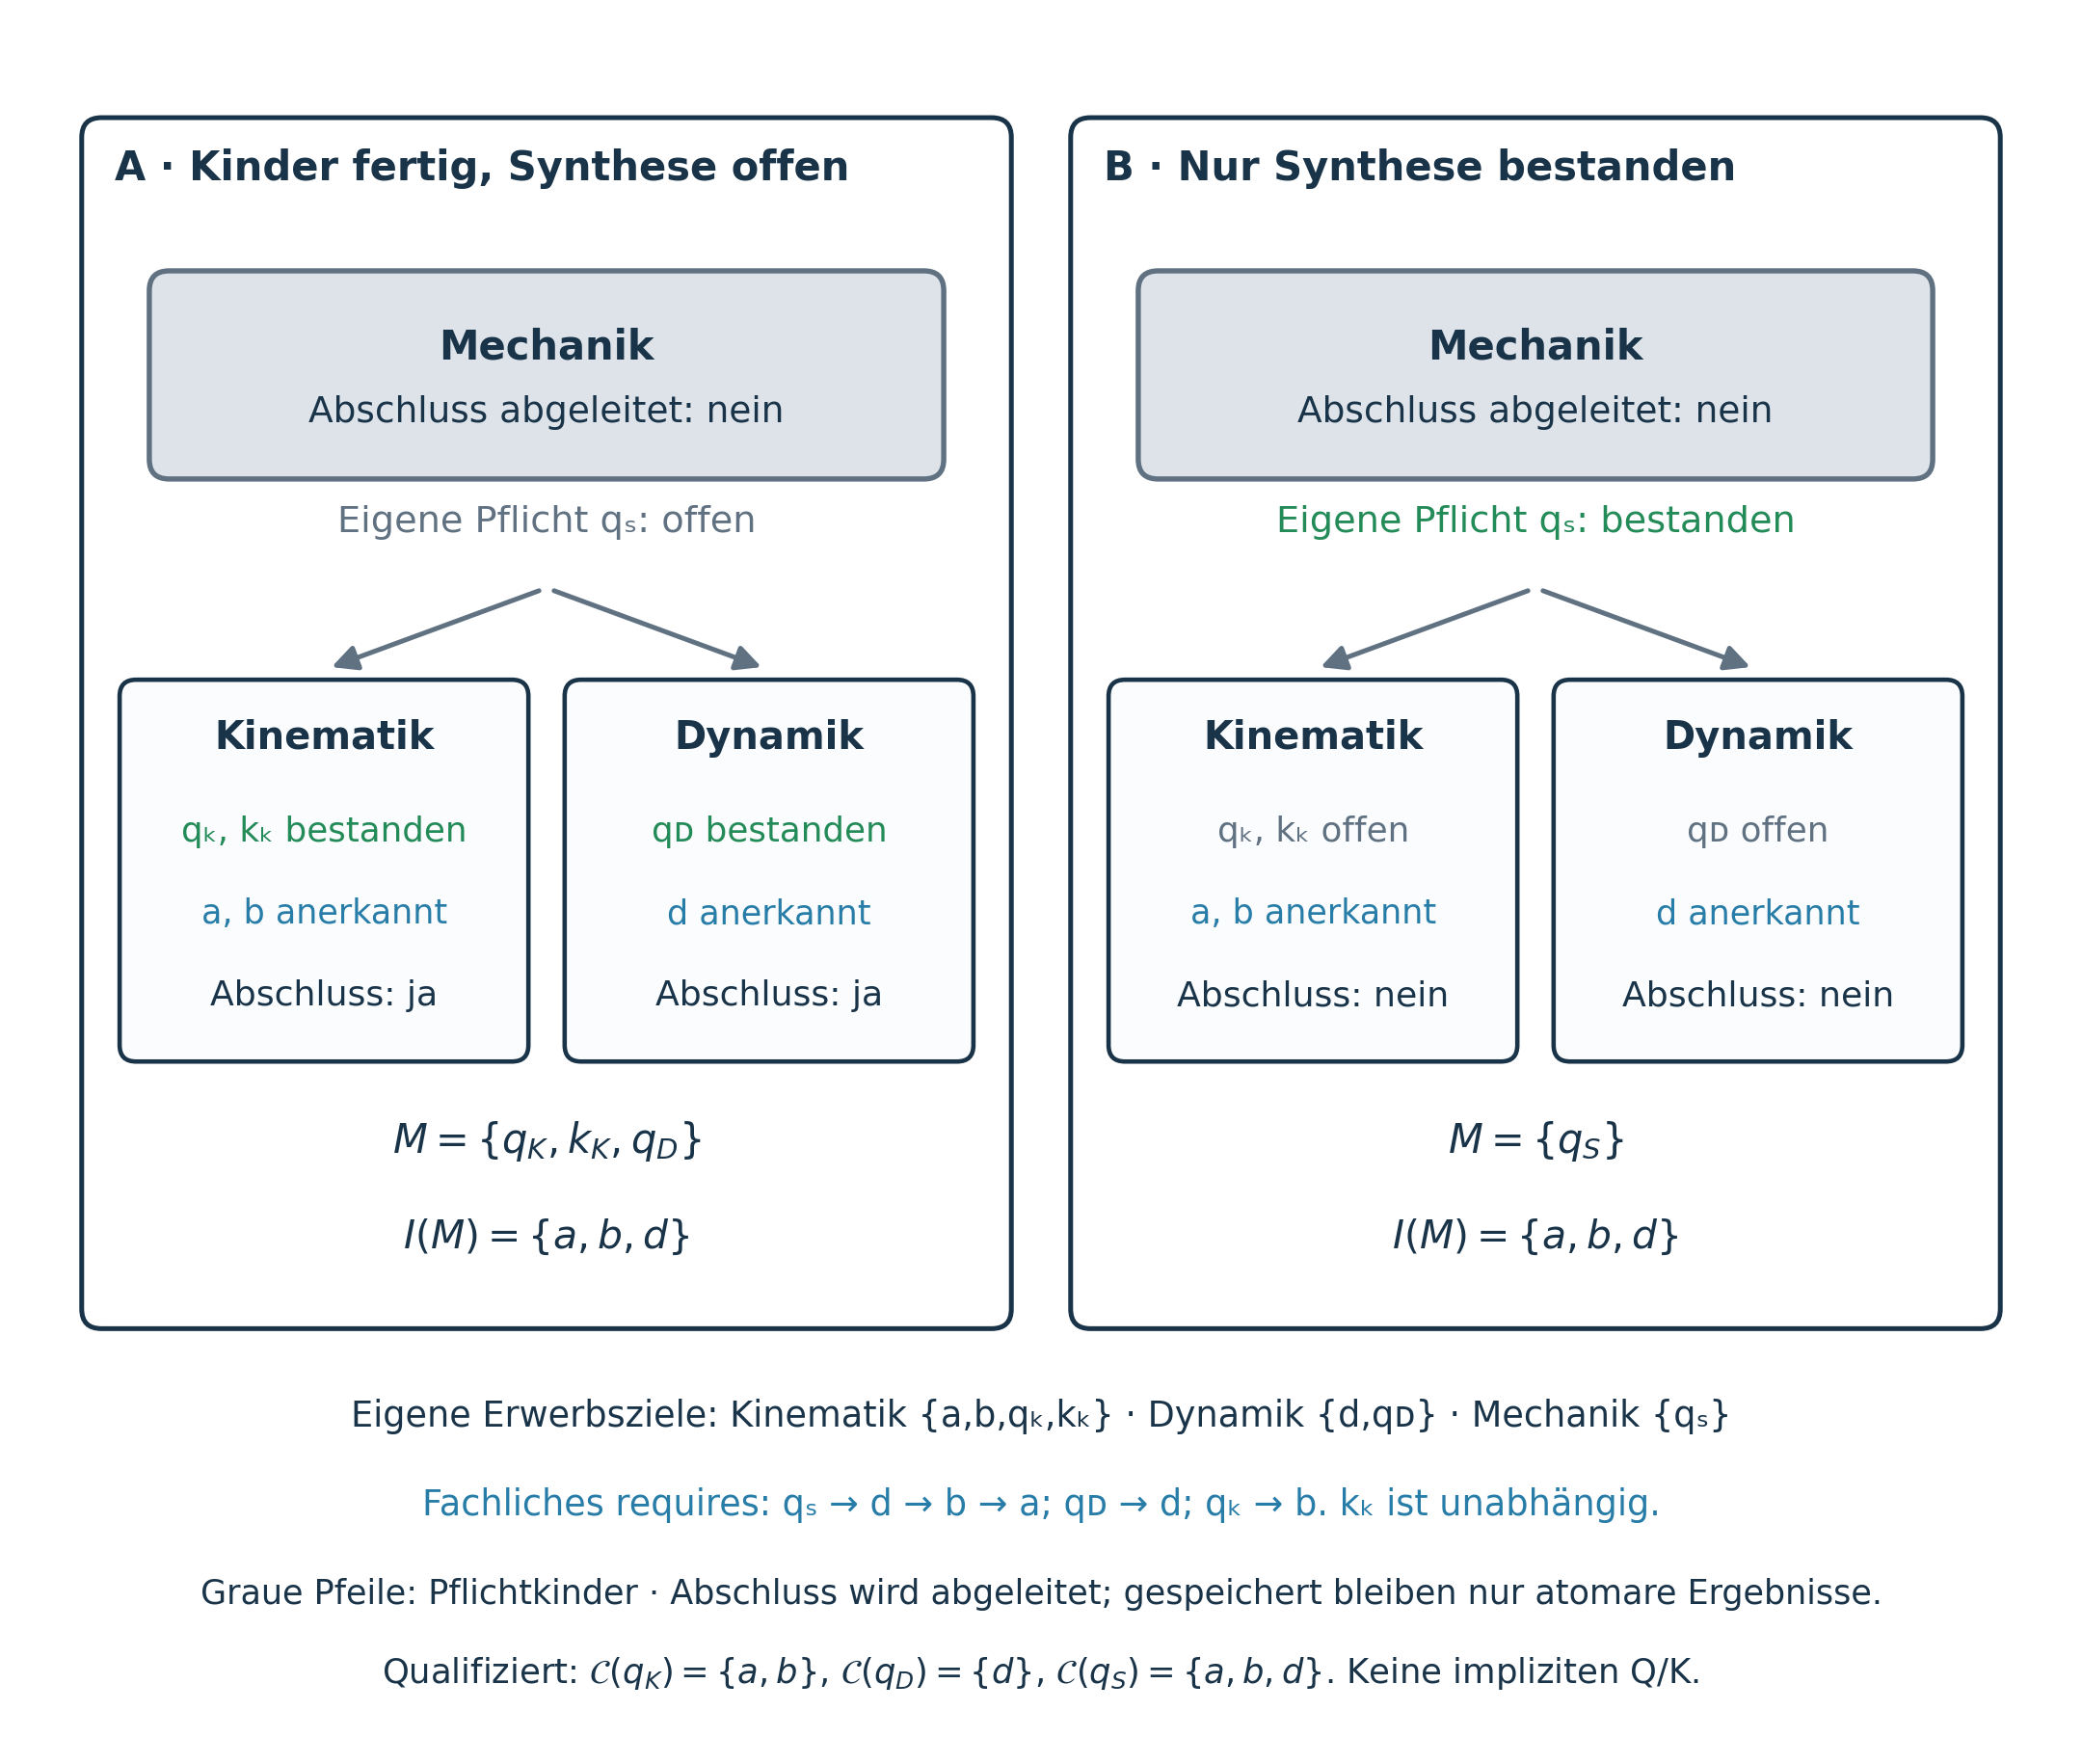
\includegraphics[width=\linewidth]{assets/graph-definition/16-recursive-learning-unit.png}
\caption[Mechanik als rekursive Lerneinheit]{Illustrative Hierarchie mit
eigenständigen Kindverträgen. Fall~A (links): Beide Kinder sind vollständig
abgeschlossen, ihre Kompetenzen global anerkannt; die offene
Syntheseprüfung \nd{q_S} hält allein den Elternabschluss offen.
Fall~B (rechts): Nur die Elternprüfung ist bestanden. Sie erzeugt keine
Kindprüfungen, keinen Kartenabruf und keine Anerkennung der
Kindkompetenzen. Graue Pfeile zeigen ausschließlich die
Einheitshierarchie; die fachlichen Kanten stehen getrennt darunter.
Im Bild sind \nd{q_K}, \nd{q_D} und \nd{q_S} Prüfungsziele, \nd{k_K} ist
ein Memorierziel, und \nd{a}, \nd{b}, \nd{d} sind Inhaltsziele.
\glqq Kind-I\grqq{} und \glqq Eltern-I\grqq{} meinen die implizite Menge
$I_U$ der jeweiligen Einheit.}
\label{fig:recursive-unit}\end{figure}
\FloatBarrier

\subsection{Anerkennung vor dem Gesamtabschluss}
Eine passende bestandene Prüfung kann die eigenen Inhaltsziele
einer Einheit anerkennen, bevor eine davon unabhängige Karte oder eine andere
Kindeinheit abgeschlossen ist. Diese Anerkennung ist global wirksam. Eine
noch offene Syntheseprüfung der Elterneinheit nimmt sie nicht zurück.

Für jede Einheit wird deshalb nur die Anerkennung ihrer \emph{eigenen}
Ziele berechnet, soweit sie keine Prüfungs- oder Memorierziele sind. Die
Elterneinheit bildet aus allen Nachfahren
keinen neuen vergrößerten Anerkennungsumfang. Sonst könnte ihre Prüfung
untergeordnete Prüfungs- oder Kartenpflichten unzulässig umgehen.
Eine Elternprüfung kann zusätzliche Integration belegen, ohne die
ursprüngliche Nachweisbedeutung der Kindverträge rückwirkend zu erweitern.
Die genaue Formel und ihre Inhaltsbedingungen stehen in
Abschnitt~\ref{sec:assessment}.

\subsection{Voraussetzungen und die Grenze einer Einheitsfolge}
Zwei Arten von Voraussetzungen sind zu unterscheiden:
\begin{itemize}
\item Ein atomarer \code{requires}-Bezug auf eine Kompetenz fordert diese
 Kompetenz. Er fordert nicht automatisch den Abschluss ihrer gesamten
 Einheit.
\item Eine \emph{Einheitsvoraussetzung} ist eine ausdrücklich autorisierte
 Voraussetzung zwischen ganzen Lerneinheiten. Sie bedeutet
 \emph{Vollabschluss} der vorausgesetzten Einheit und gehört zum
 Kompositionsvertrag außerhalb der bisherigen Grundrelationen $C$ und $R$.
\end{itemize}
Diese Aussagen dürfen weder im Compiler noch im Coach verwechselt werden.

Die Einheitshierarchie muss azyklisch sein. Wer darüber hinaus eine
ungeteilte Abschlussfolge von Einheiten behauptet, in der jede Einheit
vollständig abgeschlossen wird, bevor die nächste beginnt, muss auch deren
Voraussetzungsgraphen prüfen. Ein atomarer DAG genügt nicht: Bei
$a\to b\to c$, $\Own(U)=\{a,c\}$ und $\Own(V)=\{b\}$ braucht $U$ die
Einheit $V$ wegen $a\to b$ und $V$ die Einheit $U$ wegen $b\to c$. Nach
Zusammenfassung entsteht also eine Abhängigkeit in beide Richtungen. $U$
und $V$ sind so keine gültige ungeteilte Vollabschlussfolge. Die Diagnose
erfordert eine andere Gruppierung oder einen ausdrücklich feineren
Erwerbsablauf; sie erzeugt keine stillschweigenden Einheitssperren aus
atomaren Kanten.

Die atomare Normalform und die Migrationsreihenfolge aus
Abschnitt~\ref{sec:validity} gelten weiterhin: vollständige atomare
Voraussetzungen sichern, dadurch redundante nichtatomare Anforderungen
entfernen und erst danach die atomare Relation transitiv reduzieren.
Daraus folgt noch keine neue Minimalitätsregel für eine erst zu
beschließende Relation von Einheitsvoraussetzungen.

\begin{principle}{Zugangsprofil noch offen}
Eine fachliche Erwerbsordnung ist noch keine technische Zugangssperre.
Ob und wann eine Einheitsvoraussetzung einen harten Zugangsschutz, eine
\emph{Einheitssperre}, erzwingt, und wie dann direkte Prüfungsversuche
behandelt werden, ist \textbf{noch nicht entschieden}. Ein solches Profil
wäre gesondert zu beschließen und zu prüfen. Die Einheitendefinition führt
es nicht ein.
\end{principle}

Nur \emph{falls} später ein ausdrückliches Sperrprofil gewählt wird, könnte
man für autorisierte Vorgängereinheiten $\operatorname{Pred}(U)$ definieren:
\[
 \operatorname{Open}(U)=\bigwedge_{V\in\operatorname{Pred}(U)}
      \operatorname{Cleared}(V),\qquad
 \operatorname{Cleared}(U)=\operatorname{Open}(U)\land\Complete(U).
\]
$\Complete$ beschreibt die vorhandenen Nachweise, $\operatorname{Cleared}$
nur die bedingte Kurspolitik. Weder das Öffnen noch diese abgeleitete
Freigabe vergibt Mastery. Ob direkte Prüfungen bei geschlossenem Zugang
zulässig bleiben, entscheidet diese bloße Beispielgleichung nicht.

\sources{%
\srcref{docs/concept/skill-graph/learning-units.md}{Lerneinheiten};
\srcref{docs/concept/skill-graph/learning-unit-progression.md}{Einheitsfolge und Zugangsprofile};
\srcref{docs/concept/skill-graph/graph-definition.md}{Graph Definition, Abschnitt 12};
\srcref{docs/concept/skill-graph/assessment-gated-completion.md}{Anerkennung und globaler Abschluss}.}

\clearpage
\ohead{Optionale Erwerbs- und Zeitplanung}
% SPDX-License-Identifier: Apache-2.0
\section{Optionale Erwerbs- und Zeitplanung: Reihenfolge und Budget}
\label{sec:levels}
Dieser Abschnitt beantwortet zwei Planungsfragen: Lassen sich die Ziele
eines Plans in der vorgesehenen zeitlichen Reihenfolge überhaupt erwerben,
und reicht die verfügbare Zeit dafür? Beide Prüfungen rechnen mit einem
Plan, nicht mit dem Lernzustand einer Person.

\begin{principle}{Status: zusätzliches Planungsprofil}
Lerneinheiten tragen den fachlichen Zusammenhang und ihren rekursiven
Abschluss. Ein optionaler Zeitplan ordnet deren Erwerbsziele auf
Planungsstufen, etwa Schuljahre oder Semester, und prüft verfügbare Zeit.
Diese Zuordnung ist keine Definition der Lerneinheiten. Sie verändert weder
Grundgraphgültigkeit noch gespeicherte Mastery und führt keine technischen
Einheitssperren ein. Ein produktiver neuer Budgetvalidator wird nicht behauptet.
\end{principle}

Eine fachliche Einheit kann in verschiedenen Bildungsgängen zu anderen
Zeiten erworben werden. Eine Planungsstufe bezeichnet hier nur einen
geplanten Zeitraum, bildhaft eine Bauetappe: Kompetenzen bleiben die
Bauteile, und ihre fachlichen Voraussetzungen bleiben erhalten. Es folgt
daraus keine Pflicht, erst alle Fächer eines Kalenderjahres abzuschließen,
bevor irgendein späteres Ziel zugänglich wird.

\subsection{Plan, Eintrittsbasis und eindeutiger Ersterwerb}
Für einen aufgelösten Plan $\pi$ seien
\begin{align}
 T_\pi&\subseteq A &&\text{geplante Erwerbsziele},\\
 B_\pi&\subseteq A\setminus T_\pi &&\text{ausdrücklich angenommene Eintrittsbasis},\\
 n_\pi&\in\N_{>0},\qquad
 \ell_\pi:T_\pi\to\{1,\ldots,n_\pi\} &&\text{Planungsstufe}.
\end{align}
Der Plan nennt also, was erworben werden soll ($T_\pi$), was beim Eintritt
als vorhanden angenommen wird ($B_\pi$) und in welcher der $n_\pi$
Planungsstufen jedes Ziel erstmals erworben wird ($\ell_\pi$).
Die Planungsstufen und ihre Präfixe sind
\[
 S_i=\{g\in T_\pi\mid\ell_\pi(g)=i\},\quad
 S_{<i}=\bigcup_{j<i}S_j,\quad S_{\leq i}=\bigcup_{j\leq i}S_j.
\]
Diese zeitliche Zuordnung (Abbildung~\ref{fig:levels}) referenziert die
fachliche Ersterwerbszuordnung der Lerneinheiten, ersetzt sie aber nicht. Jedes Ziel wird im Plan
einer ersten Planungsstufe zugeordnet. Ein anderer
Bildungsgang darf es anders platzieren. Spätere Wiederholung, Vertiefung oder
Anwendung sind zusätzliche Aktivitäten, keine neue Zielidentität.
$B_\pi$ ist eine Planungsannahme; sie schreibt keine Lernergebnisse.
Persönliche Lücken in dieser Basis brauchen eine eigene Diagnose und
zusätzliche Lernzeit.

\begin{figure}[htbp]\centering
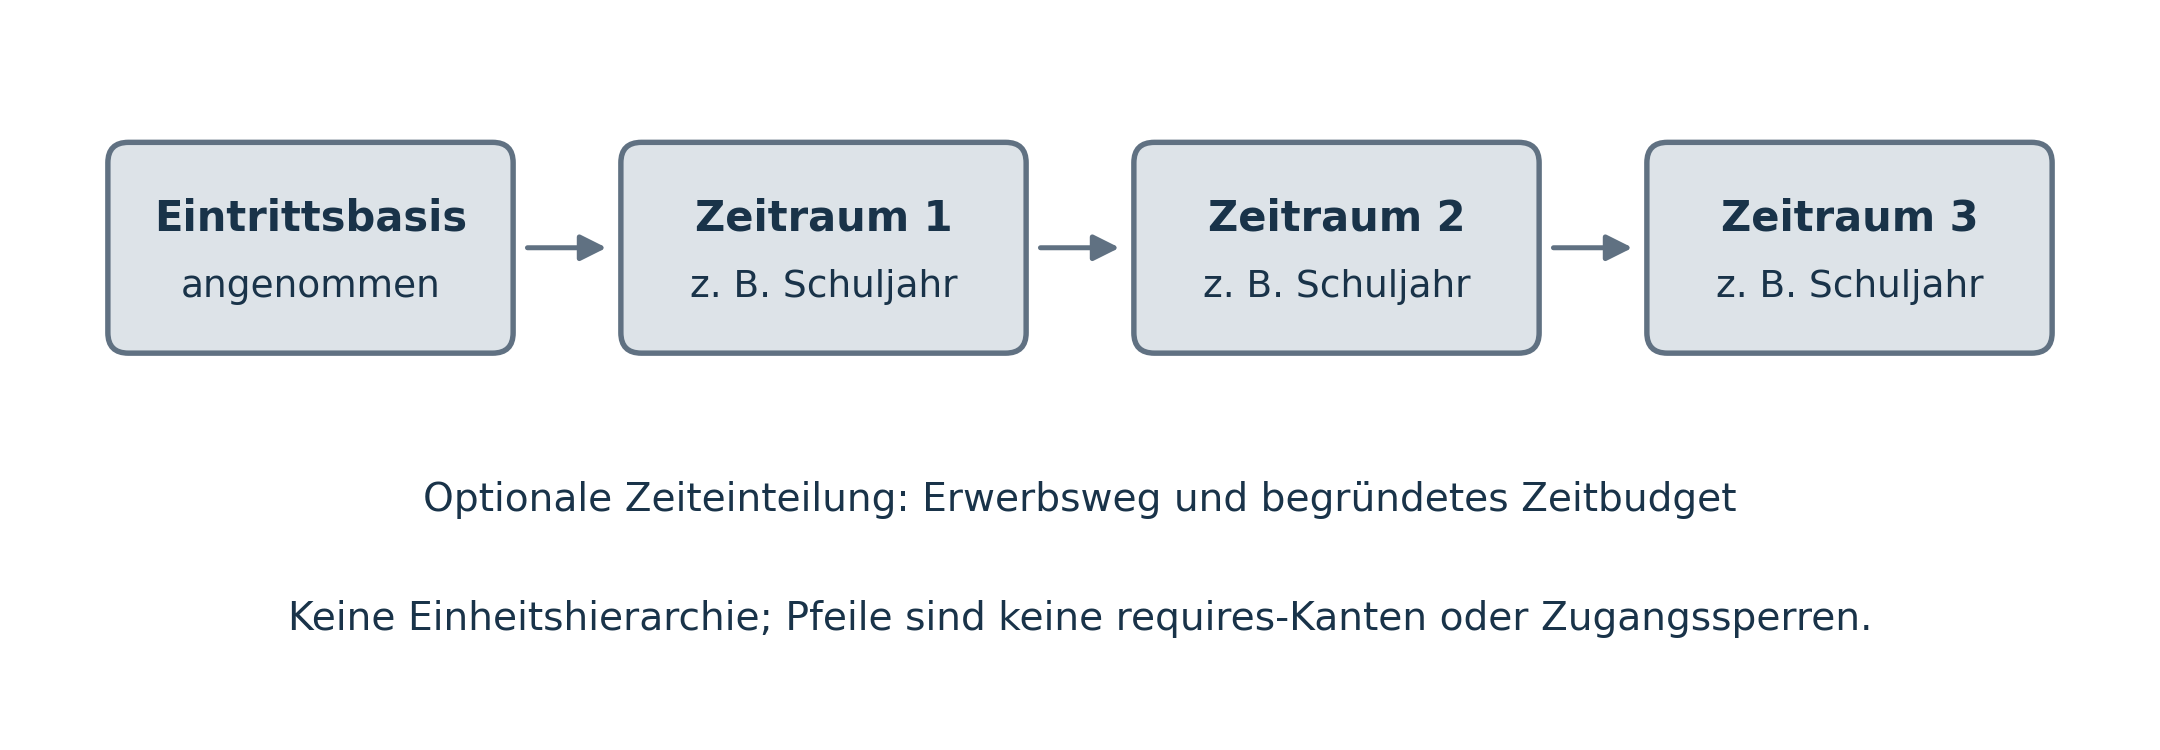
\includegraphics[width=.85\linewidth]{assets/graph-definition/12-calendar-planning.png}
\caption[Optionale kalenderbezogene Planungsstufen]{Die zeitliche
Reihenfolge ist keine rekursive Einheitshierarchie. Pfeile sind keine
\code{requires}-Kanten und führen keine Zugangssperren ein.}
\label{fig:levels}\end{figure}

\subsection{Strukturelle Machbarkeit durch einen Abschlusszeugen}
\label{sec:witness}
Die angenommene Eintrittsbasis setzt eine Planungsgrenze: Ihre frühere
Erwerbsgeschichte wird nicht rekonstruiert. Nur für den hypothetischen
Planungstest sei deshalb
\[
 \Rat^{\pi}=\{(a,b)\in\Rat\mid a\notin B_\pi\}.
\]
$\Frontier_\pi$ ist die Frontier aus \eqref{eq:frontier} mit dieser
Relation und ihrer vollständigen transitiven Hülle. Alle Ziele und früheren
Planungsstufen behalten ihre transitiven Anforderungen; nur an deklarierten
Eintrittskompetenzen endet die Planungsrekonstruktion. Diese Ausnahme
erlaubt keinen Stopp an Mastery-Zwischenzielen im wirklichen Lernzustand.

Ein \emph{Abschlusszeuge} einer Planungsstufe ist eine Reihenfolge ihrer
Ziele, in der jedes Ziel verfügbar ist, sobald es an der Reihe ist.
Eine Planungsstufe $S_i$ mit $s_i$ Zielen ist strukturell machbar, wenn
sich ihre Ziele als $a_1,\ldots,a_{s_i}$ aufzählen lassen, sodass
\begin{equation}
 a_j\in\Frontier_\pi\!\left(B_\pi\cup S_{<i}\cup
                         \{a_1,\ldots,a_{j-1}\}\right)
 \qquad(1\leq j\leq s_i).
 \label{eq:level-witness}
\end{equation}
Setzt etwa $g$ das Ziel $p$ voraus, liegen beide in derselben
Planungsstufe und sind ihre übrigen Voraussetzungen schon erfüllt, dann ist
die Reihenfolge $p,g$ ein Abschlusszeuge, die Reihenfolge $g,p$ nicht.
Hier gilt der globale Prüfbereich. Vererbte, clusterbezogene und nach
Referenzauflösung fachübergreifende Anforderungen bleiben erhalten.
Ein Normalmodusfilter würde relevante Anforderungen ausblenden können.
Der hypothetische Abschlusszeuge verwendet keine direkten Prüfungssprünge
und nimmt keine implizite Anerkennung vorweg.

Zur Diagnose dienen die benötigten Atome, also der atomare Bedarf aus
\eqref{eq:demand} bezüglich der Planrelation:
\begin{equation}
 \ReqAtoms_\pi(g)=\{b\in A\mid(g,b)\in(\Rat^{\pi})^+\}.
 \label{eq:reqatoms}
\end{equation}
Aus einem Abschlusszeugen folgt notwendig
\begin{equation}
 \forall g\in T_\pi:\quad
 \ReqAtoms_\pi(g)\subseteq B_\pi\cup S_{\leq\ell_\pi(g)}.
 \label{eq:level-closure}
\end{equation}
Jedes benötigte Atom liegt also in der Eintrittsbasis oder wird spätestens
in derselben Planungsstufe erworben. Eine benötigte Kompetenz außerhalb
$B_\pi\cup T_\pi$ ist ungeplant;
ein benötigtes Ziel mit höherer Planungsstufe ist ein Reihenfolgefehler.
Voraussetzungen innerhalb derselben Planungsstufe sind erlaubt. Die
Grundgraphgültigkeit einschließlich atomar expandierter Zyklen muss vor
dieser Mengenprüfung bereits festgestellt sein. Der explizite Zeuge
verbindet die Zuordnung mit einem tatsächlich möglichen Erwerbsweg.

Ein endlicher Prüfalgorithmus startet für jede Planungsstufe mit dem
hypothetischen Stand $W^{(0)}=B_\pi\cup S_{<i}$ und wiederholt
\begin{equation}
 W^{(r+1)}=W^{(r)}\cup\bigl(S_i\cap\Frontier_\pi(W^{(r)})\bigr).
\end{equation}
Er ist erfolgreich genau dann, wenn sein Fixpunkt ganz $S_i$ enthält.
Die Verfügbarkeit eines noch offenen Ziels kann durch zusätzliche
Erfüllungen nicht verschlechtert werden. Deshalb kann jede gleichzeitig
hinzugefügte Menge auch nacheinander erworben werden. Ein vorhandener
Abschlusszeuge kann umgekehrt nicht vorzeitig an diesem Verfahren scheitern.
Das Verfahren ist ein \emph{hypothetischer} Lerndurchlauf; es ändert keine
persönlichen Daten. Im rein atomaren DAG liefert eine voraussetzungsgetreue
topologische Ordnung den bekannten Spezialfall.

\subsection{Aufwand, Reserve und Budget}
Strukturelle Machbarkeit beweist noch nicht, dass ein Schuljahr zeitlich
ausreicht. Jede Zeitbehauptung nennt Referenzlernende, Eintrittsbedingungen,
Ziel- und Wahlauswahl, Kalender, Schätzmethode und Unsicherheit.
Diese deklarierten Schätzannahmen des Plans $\pi$ fassen wir als
$\Theta_\pi$ zusammen. Für eine tatsächliche Aktivität $h$ bezeichnet
$\widehat t_h(\Theta_\pi)\geq0$ ihre unter diesen Annahmen geschätzte Dauer.
Alle Größen müssen in derselben kalibrierten Zeiteinheit vorliegen:
\begin{equation}
 \Work_\pi(i;\Theta_\pi)+\Reserve_\pi(i)\leq \Budget_\pi(i),
 \qquad i=1,\ldots,n_\pi.
 \label{eq:budget}
\end{equation}
Dabei sind $\Work\geq0$, $\Reserve\geq0$ und $\Budget>0$.
Reserve ist geschützt und wird nicht gleichzeitig als verplanbare Zeit
ausgegeben. Ein Nullpuffer ist möglich, aber offenzulegen. Bereits im
Arbeitsaufwand enthaltene Prüfungsvorbereitung oder Wiederholung darf nicht
ein zweites Mal als Reservebedarf gezählt werden.

Ein erklärtes Aktivitätenmodell kann
$\Work_\pi(i;\Theta_\pi)=\sum_{h\in\mathcal H_i}\widehat t_h(\Theta_\pi)$
verwenden. $\mathcal H_i$ enthält jeden tatsächlichen Aufwand genau einmal:
Ersterwerb, gezielte Übung, Abruf, Prüfung und weitere geplante Arbeit.
Dasselbe kanonische Atom wird nicht in Mathematik und Physik zweimal als
Ersterwerb gezählt; eine zusätzliche Anwendung in Physik kann dennoch
eigenständige Zeit kosten. Unkalibrierte \glqq Zielpunkte\grqq{} oder
\code{weight}-Werte sind keine Minutenschätzung.
Tabelle~\ref{tab:workload} veranschaulicht die getrennte Verbuchung von
Arbeit und Reserve.

\begin{table}[htbp]
\centering
\begin{tabular}{@{}lrr@{}}
\toprule
Illustrative Planung & Stunden & Bedeutung\\
\midrule
Ersterwerb & 42 & Bereits um gemeinsame Ziele bereinigt\\
Übung und Anwendung & 12 & Zusätzliche Tätigkeiten\\
Prüfung und Wiederholung & 6 & Im Arbeitsaufwand enthalten\\
Geschützte Reserve & 10 & Nicht für obige Arbeit verplant\\
Verfügbare Zeit & 75 & Nach Kalenderausschlüssen\\
\bottomrule
\end{tabular}
\caption{Rechenbeispiel: $\Work=60$ und $\Reserve=10$ passen in
$\Budget=75$. Die erfundenen Zahlen demonstrieren nur die Rechnung,
keine empirisch abgesicherte Dauer eines SkillPilot-Curriculums.}
\label{tab:workload}
\end{table}

Ein Gesamtbudget genügt nicht, wenn Fächer, Räume oder Termine eigene
bindende Grenzen haben. Für eine zusätzlich deklarierte Fächerzuordnung
müssen auch die jeweiligen $\Work_{i,s}+\Reserve_{i,s}\leq \Budget_{i,s}$
gelten, ohne Doppelzählung gemeinsam zugeordneter Zeit. Ein Kalenderplan
muss außerdem Voraussetzungen vor der konkreten Anwendung bereitstellen.

\subsection{Gültigkeitsanspruch und Abschlussgrenzen}
Ein Zeit- und Erwerbsplan ist unter diesem optionalen Profil gültig, wenn
er sowohl strukturell als auch unter seinen erklärten Annahmen zeitlich
machbar ist.
Ohne belastbare Aufwandsschätzung ist allein die strukturelle Aussage
zulässig. Der Anspruch bindet Plan, Curriculumfassung, aufgelösten Umfang
und Schätzannahmen. Er garantiert keine identische Lerngeschwindigkeit
für jede Person.

Der Abschluss der fachlichen Lerneinheit folgt den rekursiven Zieltyp- und
Kinderpflichten aus Abschnitt~\ref{sec:learning-units}. Ein Kalenderabschnitt
kann mehrere Einheiten enthalten; eine Einheit kann sich über mehrere
Kalenderabschnitte erstrecken. Aus diesem Zeitprofil folgt keine pauschale
Voraussetzung des gesamten vorigen Jahres für jedes spätere Lernziel.

\sources{%
\srcref{docs/concept/skill-graph/learning-units.md}{Lerneinheiten};
\srcref{docs/concept/skill-graph/graph-definition.md}{Graph Definition, Abschnitt 12};
\srcref{docs/concept/didactic/curriculum-time-axis-and-pacing.md}{Zeitachse und Kapazität}.}

\clearpage
\ohead{Implizite Beherrschung}
% SPDX-License-Identifier: Apache-2.0
\section{Implizite Beherrschung durch gültige lokale Prüfungen}
\label{sec:assessment}
\begin{principle}{Verbindliche Konzeptkorrektur vom 4. November 2026}
Ein ausdrücklicher Erfolg an einem gewöhnlichen Lernziel belegt Verstehen.
Eine gültige Abschlussprüfung kann selbstständige Anwendung der zugehörigen
Kompetenzen belegen. Diese implizite Beherrschung ist global ebenso wirksam:
Sie erfüllt künftige Voraussetzungen und zählt zum IST. Prüfungs- und
Memorierziele selbst bleiben ausschließlich ausdrücklich zu bestehen.
\end{principle}

Der gespeicherte binäre Zustand $m$ bleibt unverändert das einzige
Zielergebnis. Die neue Semantik leitet zusätzliche Erfüllung ab, ohne
Rückwärtsschreiben von Mastery, zusätzliche Qualifikationsdatensätze,
manuelle Freistellungsprofile oder zweite Teilprüfungen einzuführen.
Auf der geprüften Hauptlinie ist dieses Konzept noch nicht implementiert.
Maßgeblich ist die
\srcref{docs/concept/skill-graph/assessment-gated-completion.md}{aktuelle Konzeptspezifikation}.

\subsection{Vertrag, Zielumfang und geschützte Zieltypen}
Ein lokaler Vertrag gehört zu einer autoritativen Lerneinheit U aus
Abschnitt~\ref{sec:learning-units}. Er bindet deren eigene Erwerbsziele
$\Own(U)$, die kanonischen Identitäten, die Curriculumrevision und die
fachlich geprüfte Bedeutung der eigenen Prüfungen. Ihr Gesamtumfang
$T(U)$ enthält zusätzlich die Ziele der Kinder. Er ist \emph{kein}
vergrößerter Ersatz-Anerkennungsvertrag der Eltern. Ein späterer
Integrationsanspruch erweitert die Kindverträge nicht rückwirkend.
Eine Anzeige, ein temporärer Fokus oder die aktuell ausgewählten Planwurzeln
bestimmen diese Zuordnung nicht neu.

Seien $Q$ und $K$ die autoritativ bestimmten Prüfungs- beziehungsweise
Memorierziele. In diesem Kapitel bezeichnet $K$ diesen pädagogischen Typ;
die strukturellen Cluster aus dem Kernkapitel sind hier nicht gemeint.
Dann gelten
\[
 Q_U=\Own(U)\cap Q,\qquad K_U=\Own(U)\cap K,\qquad P_U=Q_U\cup K_U.
\]
$P_U$ schützt \emph{alle} eigenen Prüfungs- und Memorierziele vor
implizitem Bestehen. Ein Erfolg an einer anderen Prüfung ersetzt weder
deren eigene Prüfung noch den verifizierten Abruf ihrer Karten.
Orientierung bleibt ein eigener motivationaler Zieltyp, keine dritte
Schutzklasse. Ein Orientierungsmarker darf in $I_U$ liegen; er ist dann
abgeleitet erledigter Einstieg, kein fachlicher Kompetenznachweis und
keine Behauptung einer tatsächlich geführten Motivationsinteraktion.
Unterstützung außerhalb $T(U)$ vergrößert den Gesamtabschlussnenner nicht.
Eine Kompetenz außerhalb $\Own(U)$ wird in diesem eigenen Vertrag nicht
implizit anerkannt; für Ziele der Kinder gelten deren eigene Verträge.

Für die folgenden Formeln heißt die vollständig atomar expandierte und
vererbte Voraussetzungrelation kurz $R$. Sie umfasst auch versteckte und
fachübergreifende Unterstützung. Alle Referenzen müssen auflösbar und die
normalisierte Relation muss azyklisch sein. Die Prüfung der gesamten
Voraussetzungshülle geschieht vor einer bloßen Anzeigeeinschränkung.

\subsection{Transitive offene Nachfrage und implizite Menge}
Mit der globalen ausdrücklichen Mastery-Menge $M=\{a\mid m(a)=1\}$ sei
\begin{align}
 N_U&=\operatorname{Reach}_{R}^{*}(P_U\setminus M),\label{eq:needed}\\
 I_U&=\Own(U)\setminus(M\cup P_U\cup N_U).\label{eq:implicit}
\end{align}
Die reflexive Erreichbarkeit enthält die offenen Wurzeln selbst und
\emph{alle} ihre transitiven Voraussetzungen. Die Traversierung stoppt
\textbf{nicht} an einem gemeisterten Zwischenziel. Dadurch bleibt
$I_U$ unverändert, wenn eine redundante Kante hinzugefügt oder für die
vorgeschriebene transitive Minimalität wieder entfernt wird.
Es gilt stets $I_U\cap M=\varnothing$ und $I_U\cap P_U=\varnothing$.

Ein direkter Algorithmus besucht von den offenen geschützten Zielwurzeln
aus jeden erreichbaren Knoten und jede Kante höchstens einmal. Er benötigt
$O(|V_U|+|R_U|)$ für die vollständige Voraussetzungshülle. Eine explizite
quadratische Speicherung der transitiven Hülle ist dafür nicht nötig.

\begin{figure}[htbp]\centering
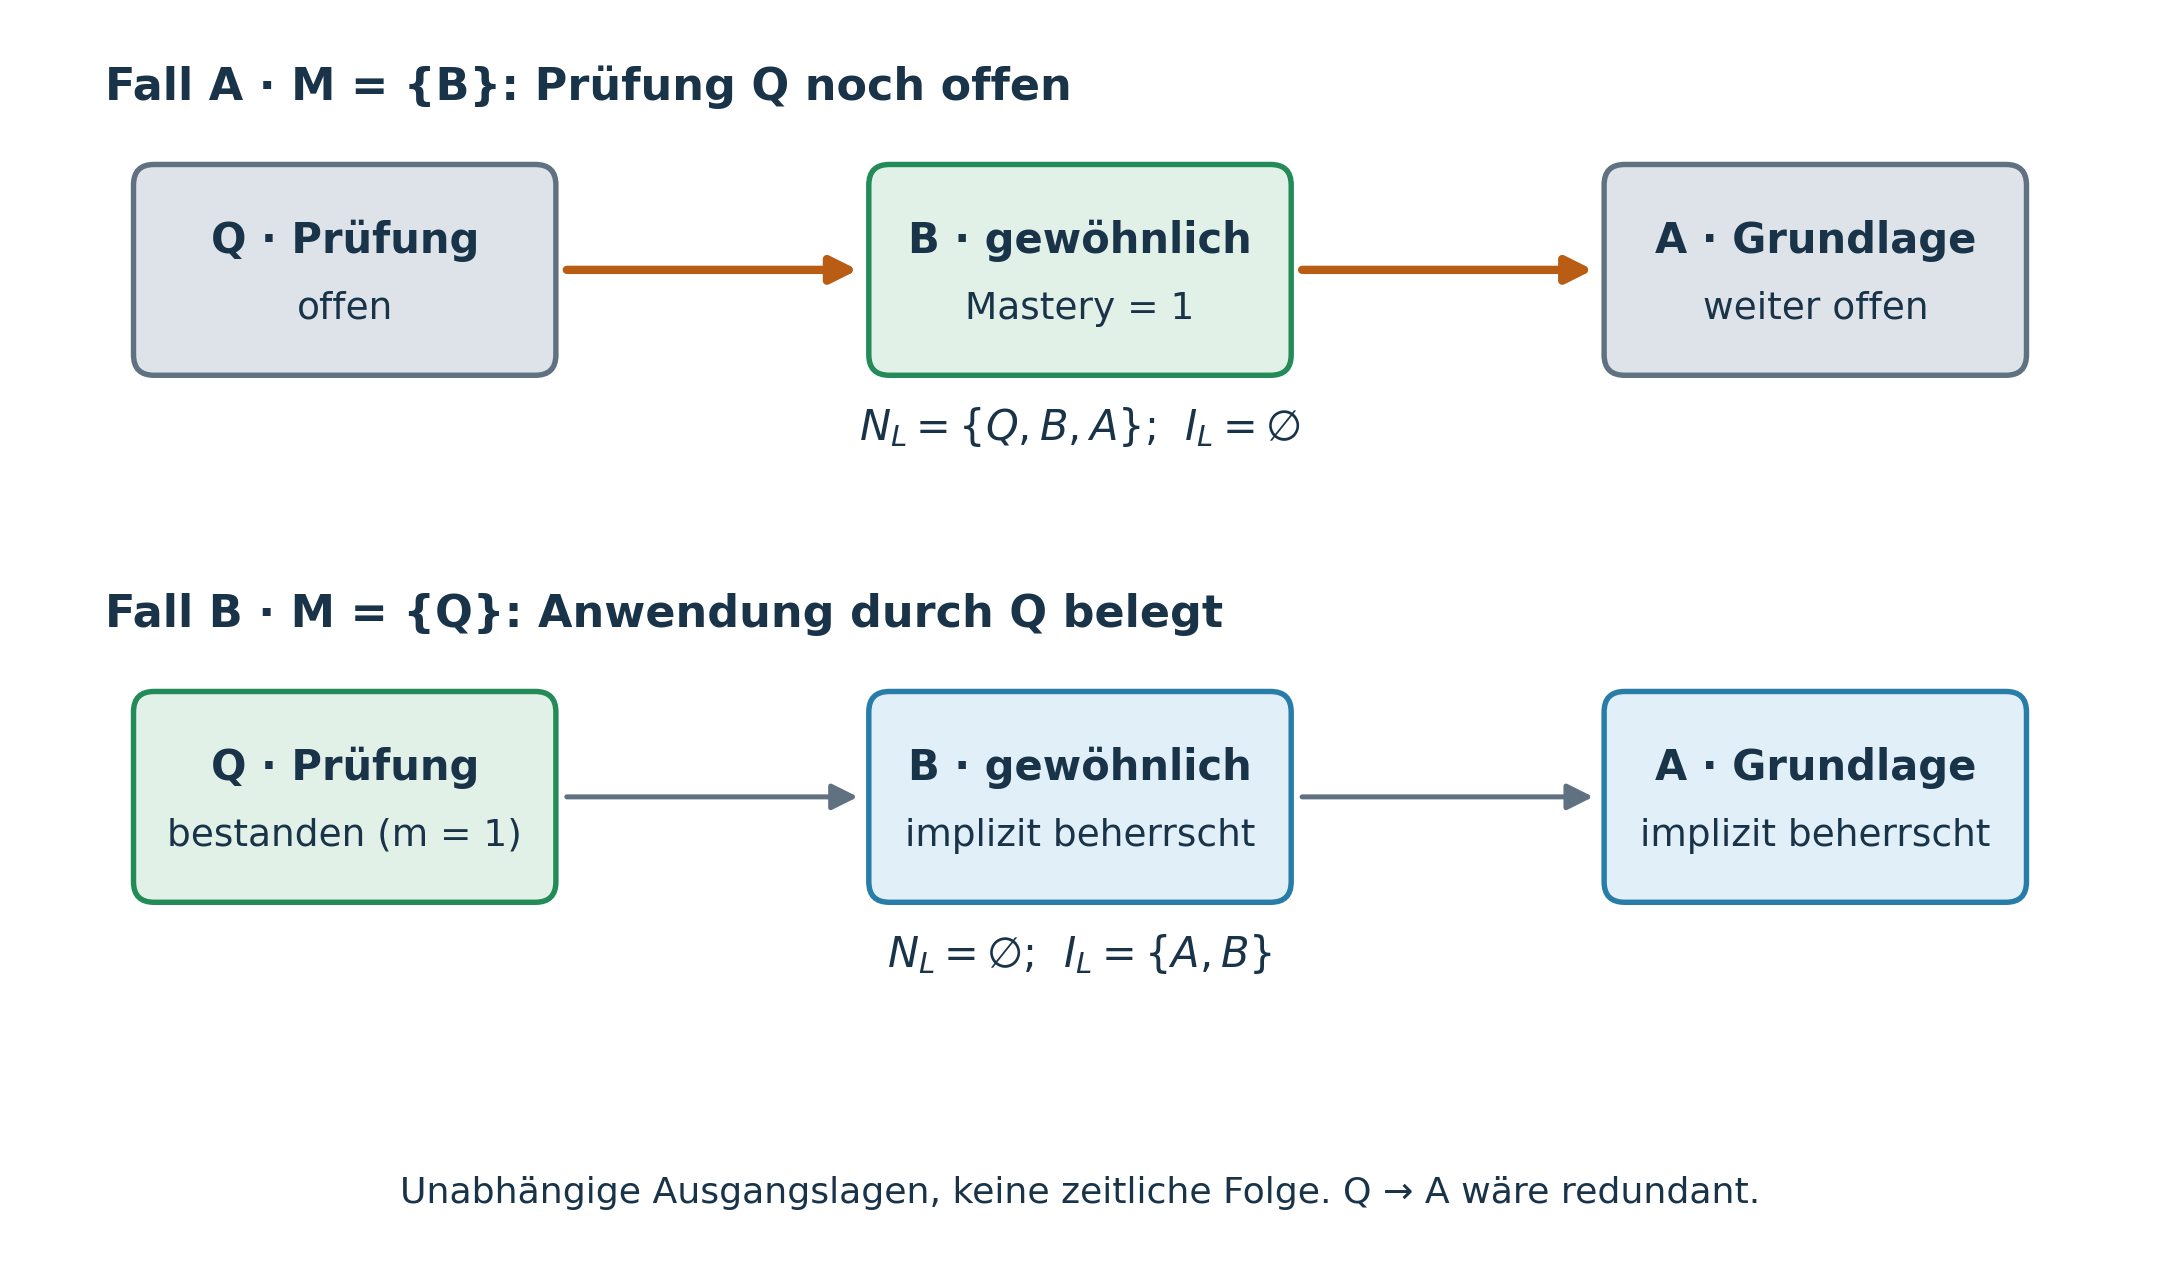
\includegraphics[width=\linewidth]{assets/graph-definition/08-transitive-demand.png}
\caption[Transitive Nachfrage trotz ausdrücklich bestandenem Zwischenziel]{Zwei unabhängige Ausgangslagen für $Q\to B\to A$: Mit
$M=\{B\}$ bleibt A offen; mit $M=\{Q\}$ trägt Q die implizite
Anwendung von A und B. Dies ist keine zeitliche Folge: Ein schon ausdrücklich
bestandenes B bliebe beim späteren Bestehen von Q in M. Die direkte Kante
$Q\to A$ wäre redundant.}
\label{fig:waivers}\end{figure}

\subsection{Warum der Graph allein noch keinen Anwendungsnachweis liefert}
Die Mengenformel darf nur für einen gültigen fachlichen Vertrag ausgewertet
werden. Jede gewöhnliche fachliche Kompetenz in $\Own(U)$ braucht einen lokalen Pfad zu
mindestens einer lokalen Abschlussprüfung aus $Q_U$. Ein Pfad allein
zu einem Memorierziel genügt nicht: Verifizierter Abruf beweist noch keine
selbstständige Anwendung. Ein bloß isoliertes
Endziel ohne lokalen Assessmentpfad ist ein Vertragsfehler, kein automatisch
beherrschtes Ziel. Das Fehlen eines späteren Verbrauchers ist allein
kein Nachweis einer Kompetenz.
Eine zusätzliche, frei wählbare Maske für \glqq anerkennungsfähige\grqq{}
Teilziele existiert nicht: Die Formel gilt für den vollständigen gültigen
eigenen Vertrag.

Für fachliche Kompetenzziele müssen die realen Aufgaben und
Bewertungsraster jede beanspruchte höhere Anwendung tatsächlich tragen.
Diese Anforderung macht einen Orientierungsmarker nicht nachträglich
zu einer prüfbaren Fachkompetenz. Wesentliche Kompetenzen dürfen nicht vollständig
fehlen und durch Punkte aus anderen Aufgabenteilen kompensiert werden.
Der lokale \code{requires}-Pfad, Titel, \code{coveredGoalIds}, eine
Bestehenspunktzahl oder die formale DAG-Gültigkeit beweisen das nicht.
Ein unabhängiges fachliches Review prüft Aufgaben, Lösungen, Bewertungsraster
und die behauptete Anwendungsabdeckung zusammen. Zu prüfen ist jede
Bestehenskombination, die ein Ziel nach der Mengenformel freigibt; die
vereinigten Inhalte aller Prüfungen allein genügen dafür nicht.

Der reguläre Prüfungserfolg bleibt derselbe binäre Erfolg der gesamten
Prüfung. Die strengere Anwendungsbedeutung liegt im vorab geprüften
Inhaltsvertrag, nicht in einem zusätzlichen pro Person zu speichernden
Qualifikationsstatus oder einer zweiten Folgeprüfung.
Ein ungeprüftes historisches Assessment erhält die stärkere Bedeutung
nicht nachträglich allein durch ein neues Diagramm oder eine Softwareänderung.

\subsection{Globale Wirkung und dauerhafte Vertragsbindung}
Die Menge $\mathcal U_{\mathrm{valid}}$ umfasst die für diese Person
dauerhaft anwendbaren autoritativen Einheitsverträge, nicht beliebige
besuchte Ansichten oder sämtliche neuesten Inhaltsfassungen. Es gilt
\[
 M_{\mathrm{eff}}=M\cup
       \bigcup_{U\in\mathcal U_{\mathrm{valid}}}I_U.
\]
Die Vereinigung umfasst nicht nur die gerade angezeigten Lerneinheiten oder den
aktuellen Personal-Curriculum-Plan. Vertrag, Revision und Nachweisbedeutung
müssen nach einem Auswahlwechsel weiter verfügbar sein. Die Ableitung wird
immer aus den ausdrücklichen Ergebnissen und ihren gültigen Verträgen
berechnet; frühere implizite Mengen werden nicht als neue Mastery-Eingaben
zurückgespeist.

Eine spätere Lerneinheit mit einer weiteren Prüfung Q2 darf eine bereits aus U1
belegte Anwendung A nicht wieder öffnen. A erfüllt vielmehr die Voraussetzung
von Q2. Bei festem Vertragsbestand kann zusätzliche ausdrückliche Mastery
$M_{\mathrm{eff}}$ nur vergrößern: Die Menge offener geschützter Wurzeln
wird kleiner, ihre transitive Nachfrage nimmt ab. Ein aus $I_U$
herausfallendes neu ausdrücklich bestandenes Ziel bleibt über $M$ enthalten.

\begin{figure}[htbp]\centering
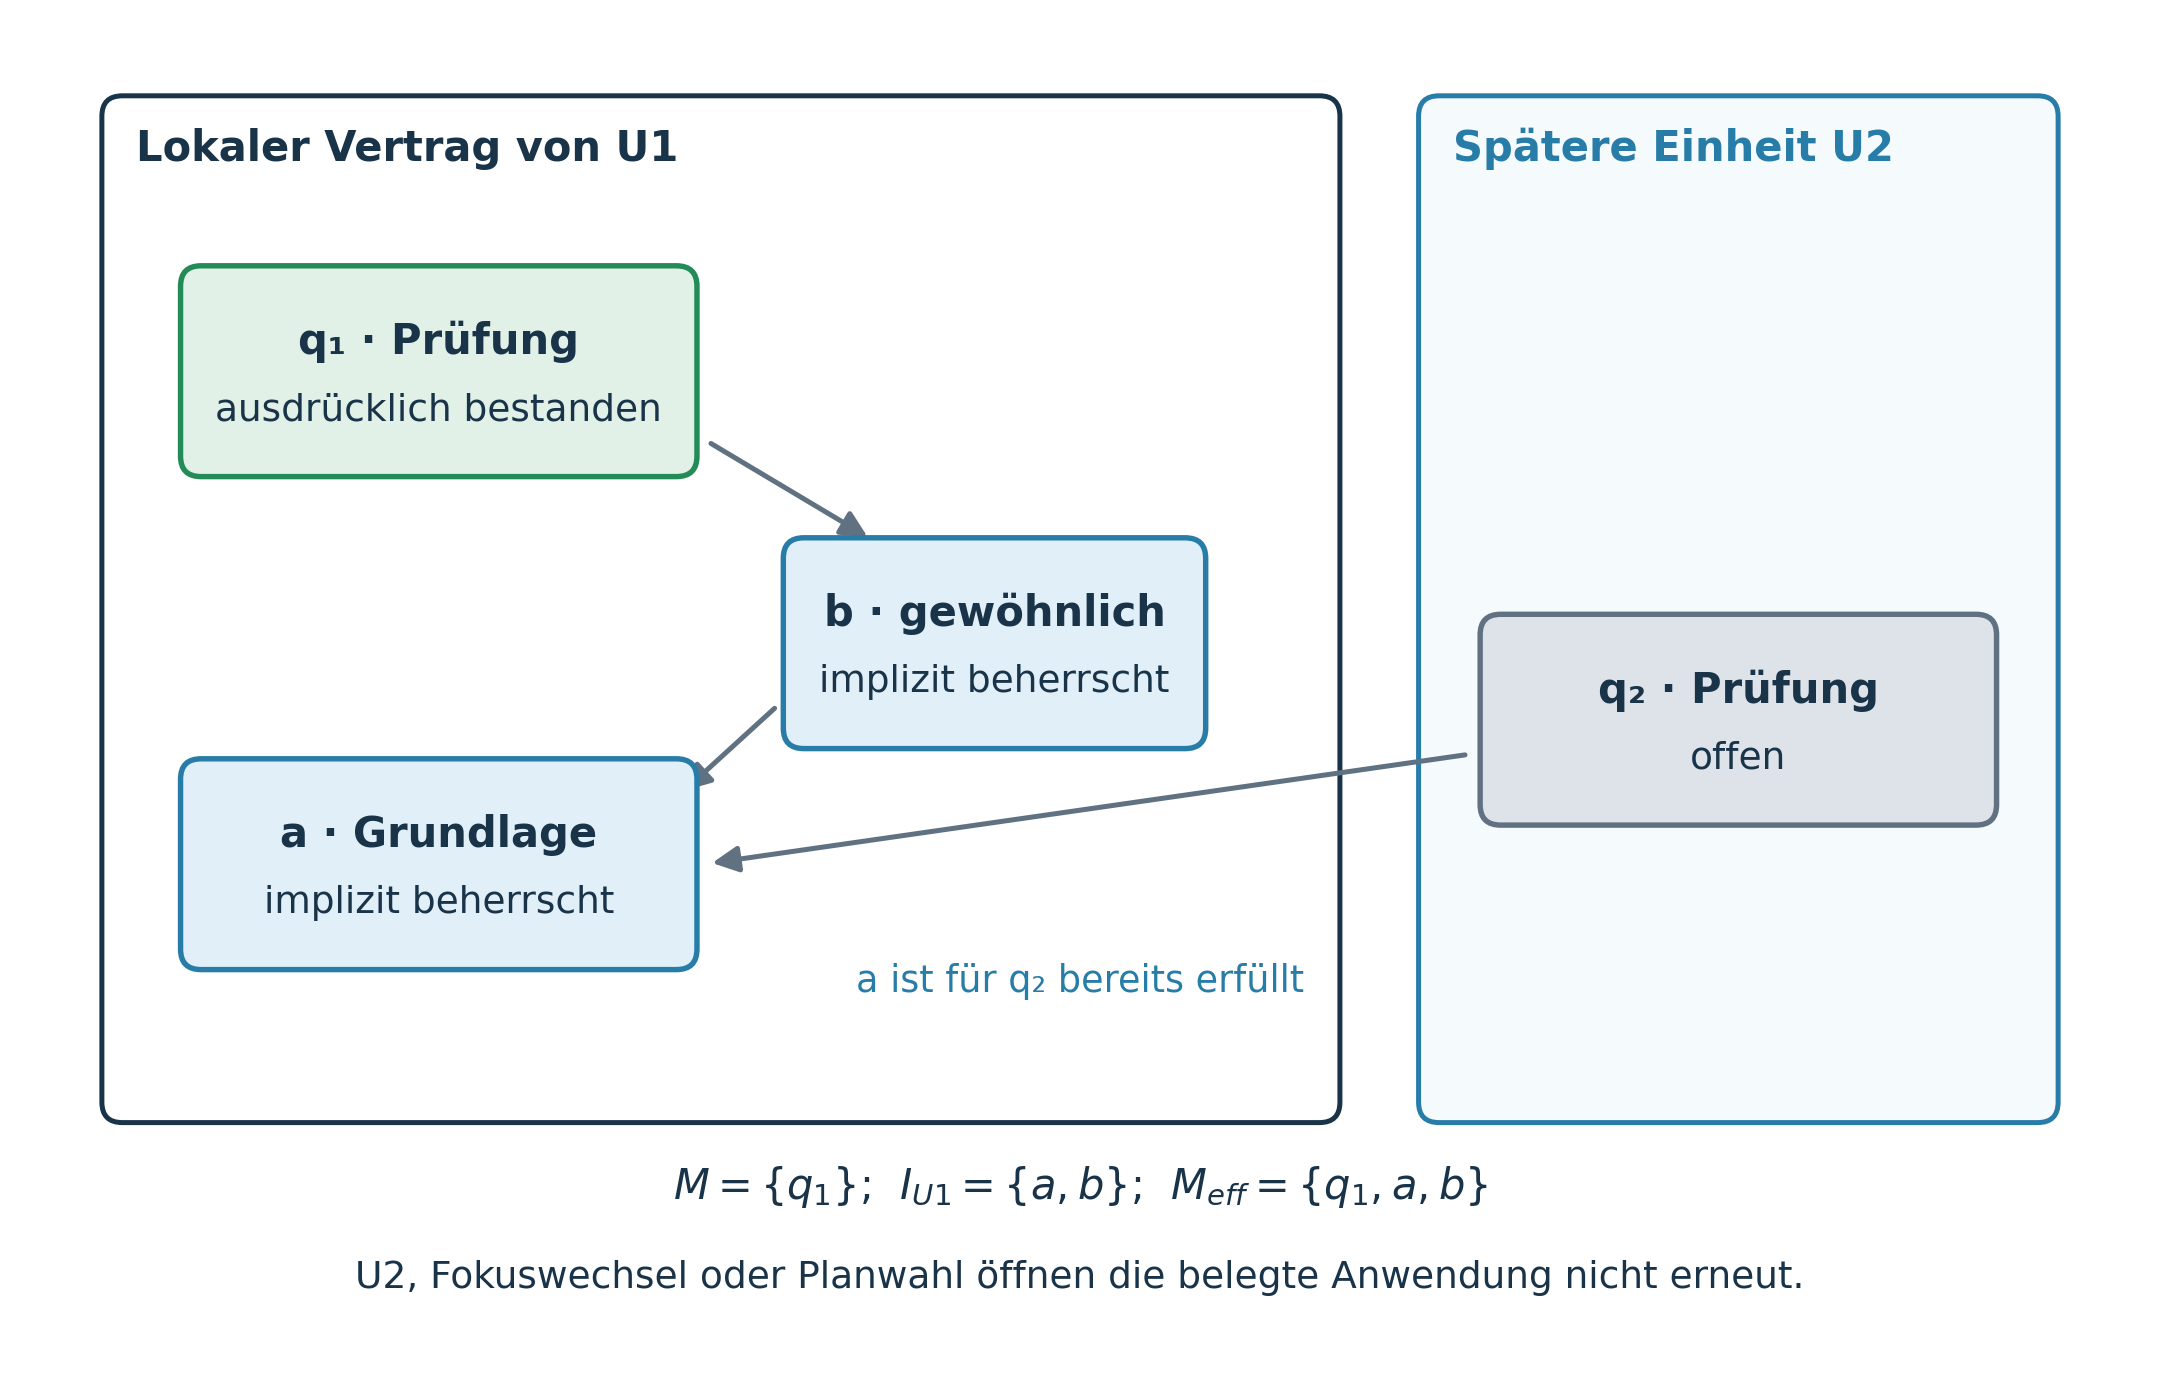
\includegraphics[width=\linewidth]{assets/graph-definition/09-local-recognition.png}
\caption[Lokale Anerkennung bleibt für spätere Lerneinheiten wirksam]{U1 erkennt A und B nach seinem eigenen gültigen Vertrag an.
Die offene spätere Prüfung Q2 verhindert diese Anerkennung nicht.
Eine neue Anzeige oder Planwahl löscht den weiter auswertbaren U1-Vertrag nicht.}
\label{fig:local-recognition}\end{figure}

Eine stabile Prüfungsziel-ID braucht eine stabile Anerkennungsbedeutung.
Wechselnde Aufgabenvarianten müssen denselben qualifizierten Vertrag erfüllen.
Neue fachliche Anerkennungsansprüche dürfen alte Prüfungs-Mastery nicht
stillschweigend aufwerten. Sie brauchen eine neue Assessmentidentität oder
eine ausdrücklich geprüfte Migration der vorhandenen Bedeutung. Dafür wird
kein zusätzlicher Qualifikationsdatensatz pro Lernendem eingeführt.
Ist die historische Nachweisbedeutung ungeklärt, bleibt der ausdrückliche
Erfolg erhalten; die zusätzliche höhere Anwendung wird nicht erfunden.
Berechtigte Ergebnis- oder Inhaltskorrekturen sind von einem bloßen späteren
Verbraucher- oder Planwechsel zu unterscheiden.

\subsection{Geschützte Ziele und vollständiger Abschluss}
Der ganze Abschluss folgt rekursiv aus Gleichung~\eqref{eq:unit-complete}:
Alle eigenen Ziele müssen erfüllt und alle Pflichtkinder abgeschlossen sein.
Bei festem globalem $M_{\mathrm{eff}}$ ist dies gleichbedeutend mit
$T(U)\subseteq M_{\mathrm{eff}}$, sofern sämtliche Kinderpflichten als
Zielpflichten in diesem Umfang enthalten sind. Bei vollständigem Abschluss
gilt für die eigenen geschützten Ziele $P_U\subseteq M$.

Sind alle eigenen Prüfungen und Karten bestanden, ist $N_U=\varnothing$;
ein gültiger eigener Anerkennungsvertrag kann damit seine gewöhnlichen
Erwerbsziele vervollständigen. Der Abschluss der Kinder folgt daraus
\textbf{nicht}. Eine eigene Syntheseprüfung der Eltern kann offen bleiben,
während gewöhnliche Kindziele bereits global anerkannt sind. Umgekehrt
ersetzt ihr Bestehen keine offene Q-/K-Pflicht eines Kindes.

Ein offenes eigenes Memorierziel verhindert den ganzen Einheitsabschluss,
blockiert aber nicht die Ableitung einer anderen gewöhnlichen Kompetenz,
solange es diese nicht transitiv benötigt. Ein offenes Memorierziel mit
$k\to^* a$ hält dagegen A im lokalen Bedarf. Auch mehrere Prüfungen mit
gemeinsamer Grundlage müssen in diesem lokalen Vertrag sämtlich aus dem
Bedarf an der Grundlage herausgefallen sein.

Dies unterscheidet Prüfungen im \emph{selben} Vertrag von einer späteren
Prüfung in einer anderen Lerneinheit (Abbildung~\ref{fig:local-recognition}).
Abbildung~\ref{fig:shared-assessments} zeigt zwei aufeinanderfolgende
Ergebnisse bei unverändertem lokalem Umfang und ohne weitere Abschlusspflichten.
\begin{figure}[htbp]\centering
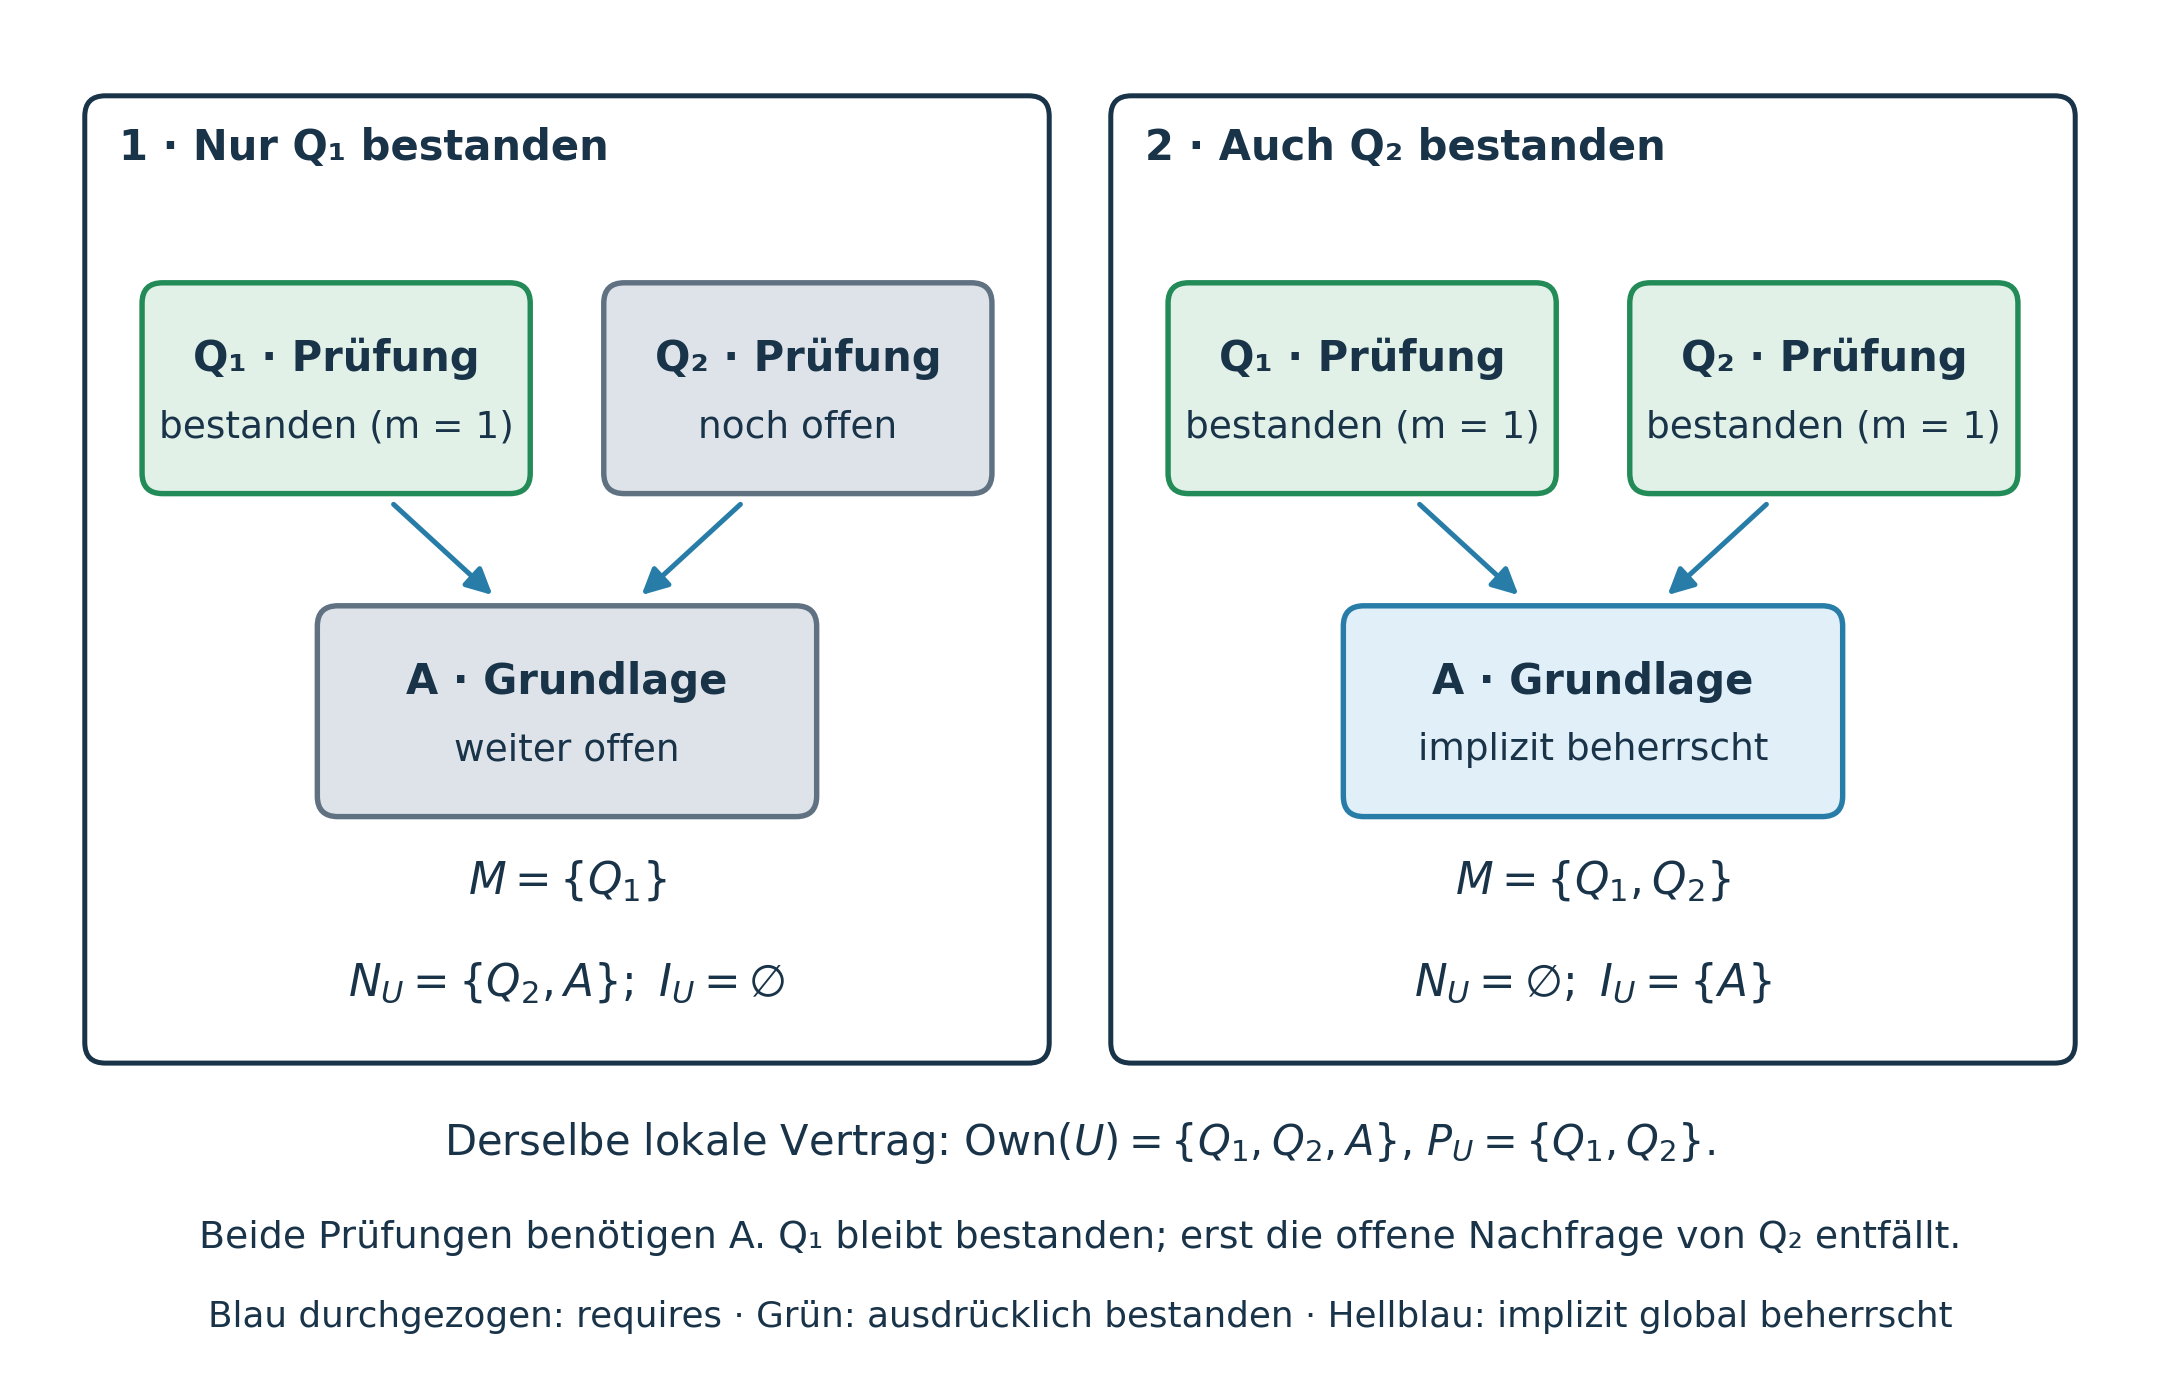
\includegraphics[width=\linewidth]{assets/graph-definition/15-shared-local-assessments.png}
\caption[Zwei lokale Prüfungen mit gemeinsamer Grundlage]{Q1 und Q2
benötigen im selben gültigen Erwerbsvertrag A. Nach Q1 bleibt A wegen der
offenen Q2 im transitiven Bedarf. Erst nach beiden Prüfungen wird A
implizit global beherrscht. Der ausdrückliche Erfolg von Q1 bleibt dabei
erhalten; es gibt hier keine weiteren geschützten Ziele.}
\label{fig:shared-assessments}\end{figure}
\FloatBarrier

\begin{figure}[htbp]\centering
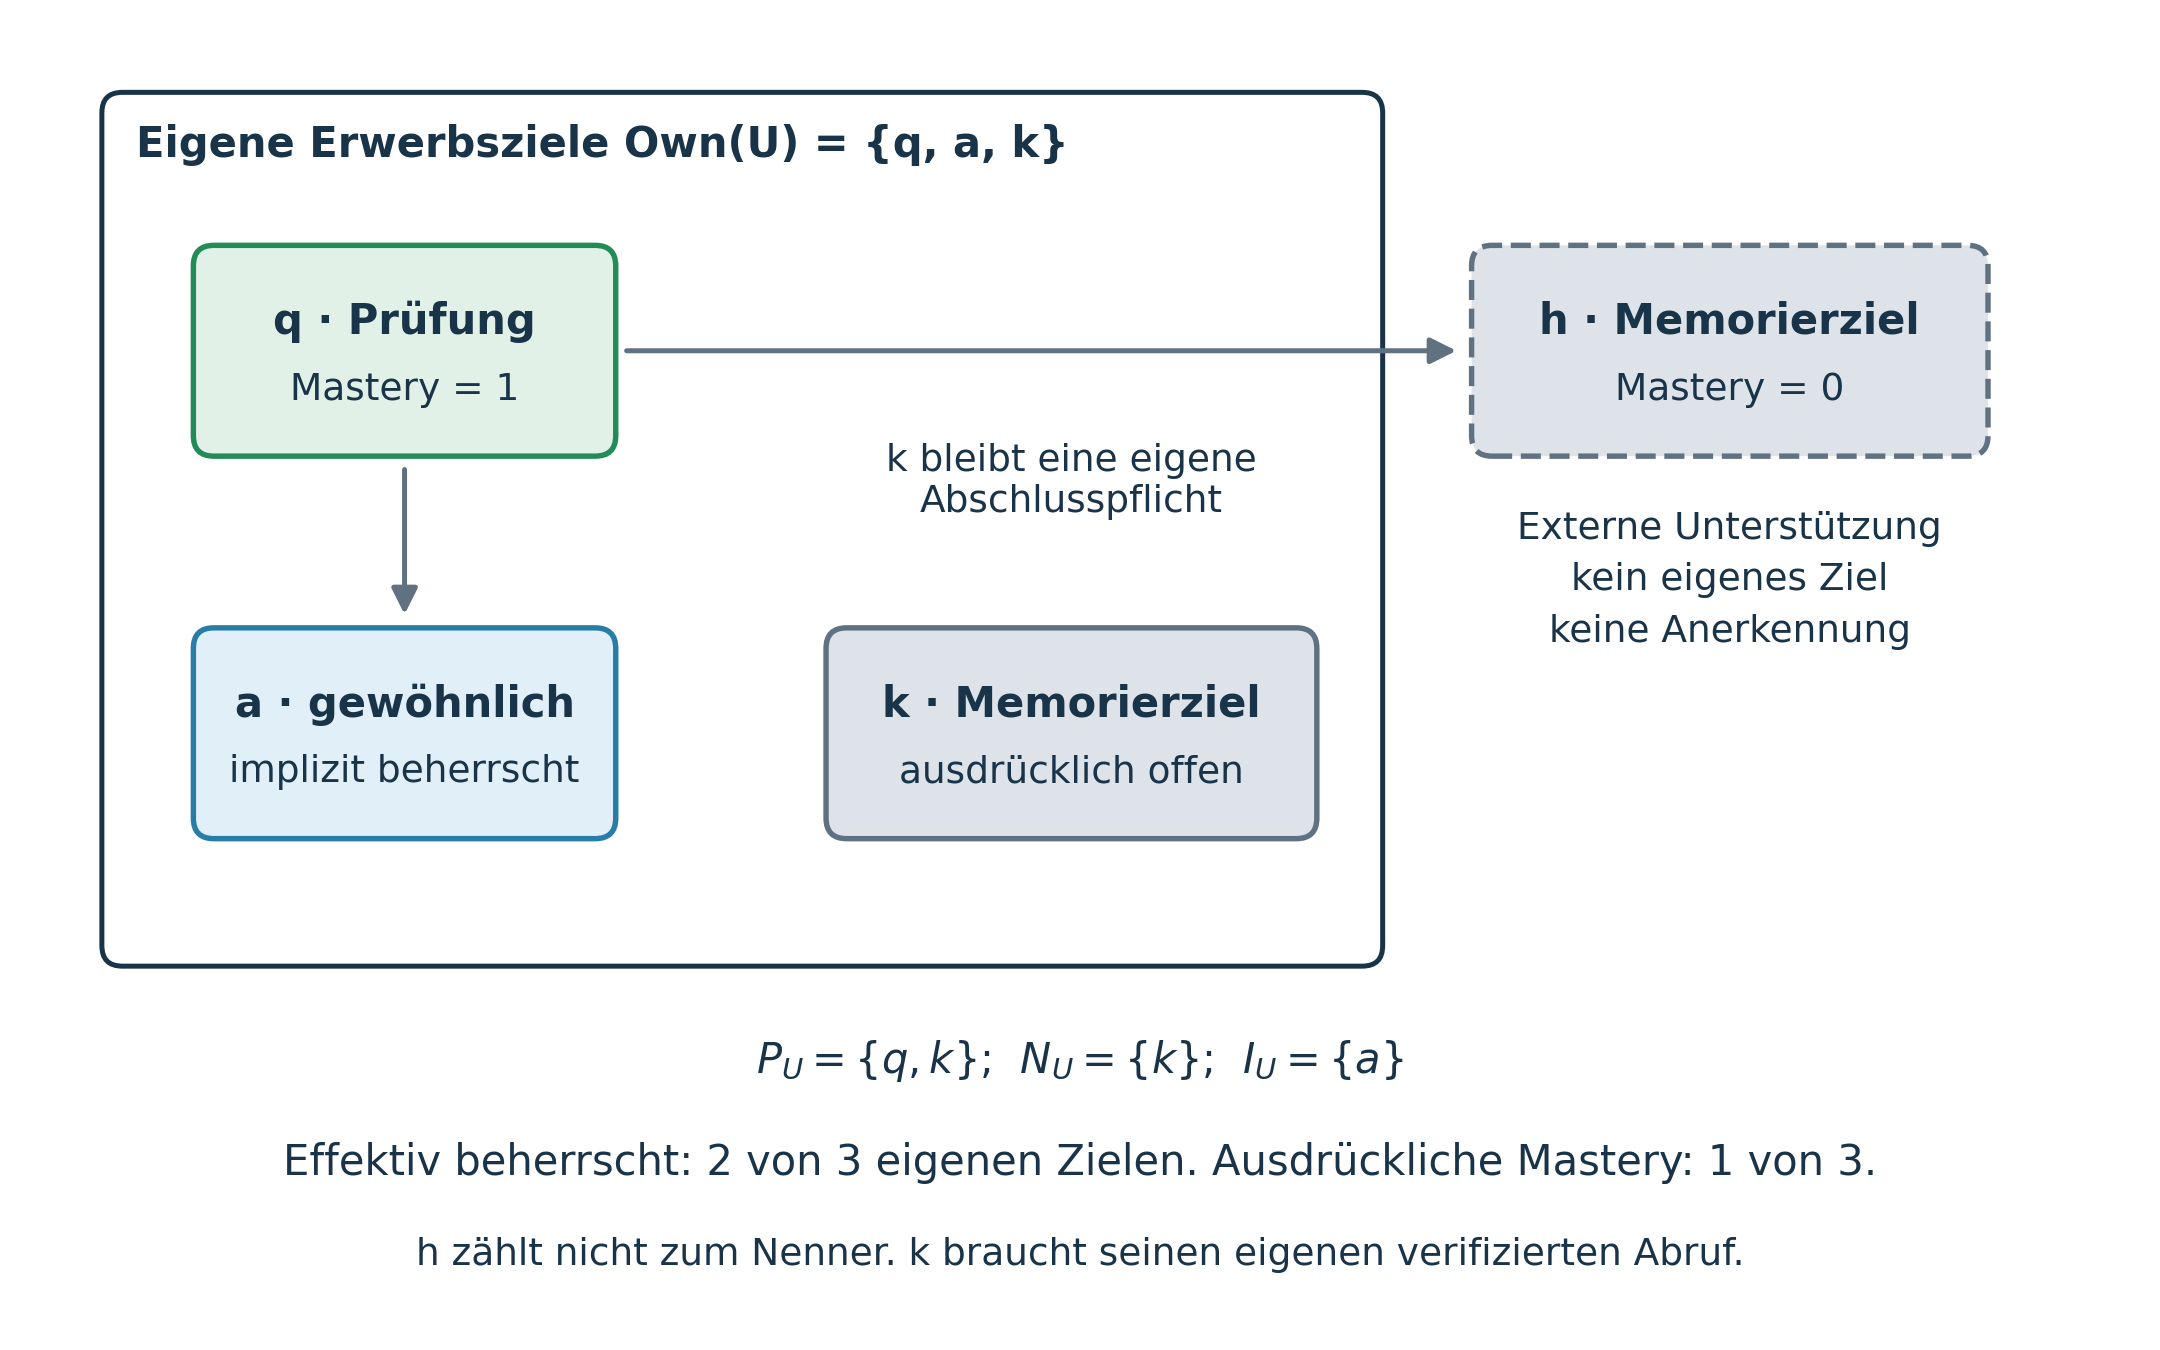
\includegraphics[width=\linewidth]{assets/graph-definition/10-protected-support.png}
\caption[Geschützte Memorierziele und externe Unterstützung]{Q ist ausdrücklich bestanden und trägt die Anwendung A.
Das unabhängige Memorierziel K bleibt offen und blockiert den ganzen
Einheitsabschluss. Unterstützung H außerhalb des Zielumfangs wird nicht anerkannt.}
\label{fig:protected}\end{figure}

Der bisherige direkte Prüfungszugriff bleibt der Ausgangspunkt des
aktuellen Lernablaufs. Aufgabenverfügbarkeit, Authentifizierung,
Sitzungszuordnung und ausdrückliche Auswahl bleiben erforderlich.
Die Entscheidung über harte Ganzheitszugänge und direkte Prüfungsversuche
unter einem solchen optionalen Profil steht noch aus
(Abschnitt~\ref{sec:learning-units}). Die rekursive Einheitendefinition
führt weder einen neuen Ausschluss noch einen verdeckten Umgehungsweg ein.
Der normale Lernzugang verwendet $M_{\mathrm{eff}}$ und die transitive
effektive Relation; die eigenständige Normal-/Strict-Fokusregel bleibt erhalten.

\subsection{Gesamt-IST und datierte Periodenereignisse}
Für eine fest benannte Plan-Zielmenge $T_{\mathrm{Plan}}$ zählt
\[
 H_{\mathrm{gesamt}}=|T_{\mathrm{Plan}}\cap M_{\mathrm{eff}}|.
\]
Die Vereinigung vor dem Schnitt verhindert Doppelzählung von expliziten und
impliziten Beiträgen sowie überlappenden Verträgen. Eine gesonderte Ansicht
nur ausdrücklicher Ergebnisse muss ihren abweichenden Zähler ausweisen.

Eine laufende Periode zählt dagegen ausschließlich tatsächlich datierte
explizite Abschlussereignisse nach ihrem Ereignisvertrag. Eine neu abgeleitete
Anwendung, mitgebrachte Vorarbeit oder nachträglich erweiterte Plananzeige
ist kein zusätzlicher tatsächlicher Abschluss in dieser Periode.
\begin{figure}[htbp]\centering
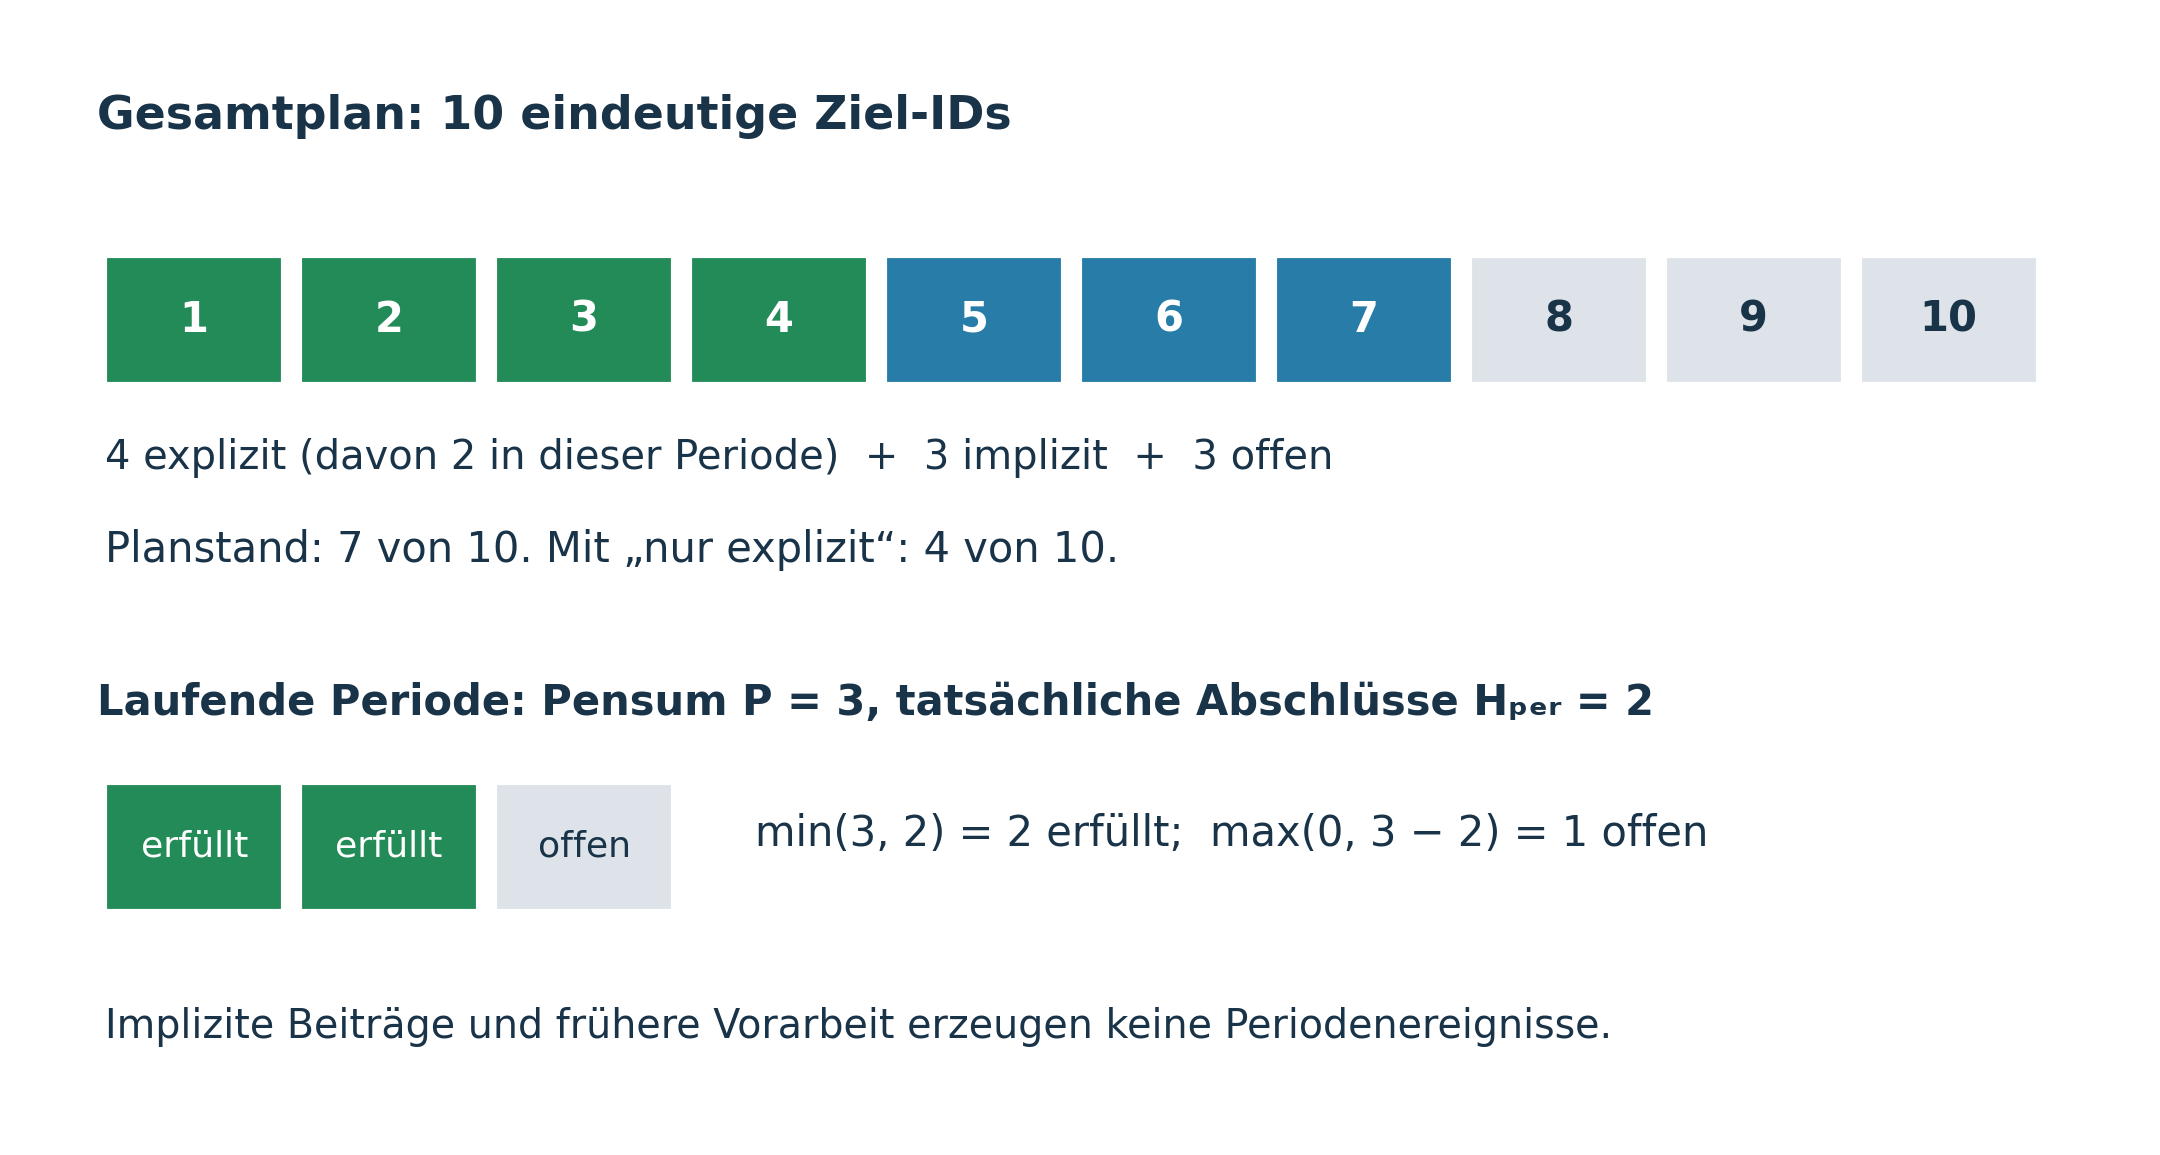
\includegraphics[width=\linewidth]{assets/graph-definition/11-plan-period.png}
\caption[Gesamtstand und datierte Periodenleistung]{Gesamtstand und Periodenleistung haben verschiedene Zähler.
Die drei impliziten Beiträge erhöhen den Gesamt-IST, erzeugen aber keine
datierten expliziten Abschlussereignisse in der laufenden Periode.}
\label{fig:period}\end{figure}

Der \srcref{docs/concept/didactic/unified-learning-plan-status.md}{gemeinsame
Lernplanstatusvertrag} beschreibt die Oberflächen. Statische Vertragsdaten
können nach Revision zwischengespeichert werden; abgeleitete Ergebnisse sind
keine zweite gespeicherte Wahrheit. Ungültige oder ungeklärte Verträge bleiben
als Einschränkung erkennbar. Maschinenprüfungen der Formeln ersetzen weder
unabhängiges Inhaltsreview noch menschliche Erprobung oder Lernwirksamkeit.

\clearpage
\ohead{Anhänge}
% SPDX-License-Identifier: Apache-2.0
\appendix
% SPDX-License-Identifier: Apache-2.0
\section{Regeln und Meilensteine}
\label{sec:rule-milestones}
Dieser Anhang ist das Nachschlageregister der Graphregeln. Er beantwortet
für jede Regel dieses Dokuments drei Fragen: Was ist verlangt, in welches
Prüfgebiet gehört die Pflicht, und was belegen die vorhandenen Prüfungen
davon tatsächlich?

\paragraph{So ist eine Zeile zu lesen.}
Jede GD-Zeile verbindet eine Pflicht mit ihrem vorgesehenen Prüfgebiet (Soll), vorhandenen Prüfungen (Ist) und deren Aussagegrenzen:
\begin{itemize}
\item \textbf{Kennung.} \code{GD-}, der Buchstabe des Dokumentteils und eine laufende Nummer. C steht für den formalen Kern, X für den Kontext, U für die Lerneinheiten, P für die Planung, A für die Anerkennung impliziter Beherrschung und D für die Dokumentanhänge.
\item \textbf{Pflicht.} Die Regel in Kurzform.
\item \textbf{Soll.} Das Prüfgebiet, dem die Pflicht zugeordnet ist: ein Meilenstein M0--M7 oder eines der Kürzel aus Abschnitt~\ref{sec:rule-code-legend}.
\item \textbf{Ist und Lücke.} Was vorhandene Prüfungen davon belegen und was offen bleibt.
\item \textbf{Fundstelle.} Der benannte Unterabschnitt, in dem die Regel steht.
\end{itemize}
Die Zeilen sind im Telegrammstil gehalten und verwenden einige Kurzwörter: Unit für Lerneinheit, Exam oder Assessment für Prüfung oder Prüfungsziel, Memory für Memorierziel oder Memorierung, Normal und Strict für Normalmodus und strikten Modus, Closure für Hülle, Scope für Prüfumfang oder Geltungsbereich, Runtime für Laufzeit, Ganzheitssperre für Einheitssperre und Humantrial für menschliche Erprobung.

\paragraph{Meilensteine und Regelfamilien.}
Die Meilensteine M0--M7 ordnen die maschinelle Curriculum-QA; Laufzeitverträge, Konzepte, optionale Profile sowie Artefakt- und Dokumentpflichten sind gesondert ausgewiesen. Die beiden vorhandenen Regelfamilien heißen \emph{Curriculum-Quality-Review} (CQR) und \emph{graph-validation rollout rule} (GVR): Sie bezeichnen curriculare Qualitätsprüfungen beziehungsweise Prüfregeln des Graphvalidators. Die Legende in Abschnitt~\ref{sec:rule-code-legend} erklärt die hier verwendeten Codes mit ihrem jeweiligen Umfang.

\paragraph{Eine Zuordnung ist kein Bestehen.}
Die Zuordnung benennt das Prüfgebiet jeder Pflicht. Die daneben ausgewiesenen vorhandenen Gates belegen ausschließlich ihren tatsächlichen Umfang. Eine verbindliche, noch nicht vollständig gegatete Regel ist keine bereits bestandene Prüfung. M0 ist ein möglicher unvollständiger Ausgangsstand, kein Gütesiegel. Profilgebundene Routengates gelten in ihren benannten QA-Scopes. Die globale Basisprüfung auf vollständige atomare Normalform und transitive Minimalität (Prüfcode G17) muss dagegen den vollständigen deklarierten kanonischen Fachbestand einschließlich relevanter fachfremder Voraussetzungen und vererbender Vorfahren erfassen; eine QA-Profil-Auswahl oder ein Teilscan genügt dafür nicht.

\paragraph{Basis vor jedem Meilenstein.}
Die vollständige atomare Normalform und eine vollständige Minimalitätsprüfung sind Sollbasis vor jedem Aufstieg zu M1–M7. Ein G17-Verstoß oder eine unvollständige Prüfung sperrt im betroffenen Fach jeden Meilensteinpass M1–M7; einzelne Quellen- oder Reviewchecks können gleichwohl für sich bestehen. Der atomare Zielzustand \(R\subseteq A\times A\) ist verbindlich. Zuerst werden vollständige atomare Voraussetzungen hergestellt oder erhalten, danach dadurch redundante nichtatomare Anforderungen entfernt und erst dann die feste atomare Relation transitiv reduziert. Ein geerbter Alternativpfad allein erlaubt keine Löschung einer atomaren Route. CQR-102 und GVR-012 bleiben direkt atomar.

\paragraph{Memorierziele.}
Kartenwiederholungen gehören zum Lernprozess. Der Abschluss eines Memorierziels benötigt seinen eigenen ausdrücklichen Prüfnachweis; spätere Fälligkeit allein nimmt ihn nicht zurück. Gewöhnliche abgeschlossene Ziele erhalten keine Wiederholungsfälligkeit oder daraus abgeleitete Mastery-Rücknahme. Eine neue Prüfungsentität oder ein neues Schema folgt daraus nicht.

\paragraph{Umfang des Registers.}
Die 143 stabilen GD-IDs erschließen alle sechs Kapiteldateien. Fundstellen verwenden benannte Unterabschnitte statt veränderlicher Zeilennummern. Laufzeitverträge, neue Anerkennungs- und Einheitensemantik, optionale Planung sowie Veröffentlichungs- und Dokumentpflichten erhalten keine erfundene Zuordnung zu M7. Fachliche Richtigkeit, menschliche Erprobung und Lernwirksamkeit bleiben eigenständige Nachweise.

\subsection{Kurzübersicht der Prüfgebiete}
\begingroup\small
\begin{longtable}{@{}P{23mm}P{64mm}P{61mm}@{}}
\toprule
Zuordnung & Prüfpflicht & Ist-Grenze\\
\midrule\endhead
M0-Basis, vor M1 & Identität, Referenzen, Struktur und Grundgraph; vollständige atomare Normalform und Minimalitätsprüfung als Sollbasis jedes höheren Meilensteinpasses. & CQR-001/002 und Graphvalidatoren prüfen Teile; kein vollständiger Strukturpass.\\\addlinespace[4pt]
M1 & Lesbares, nachvollziehbar registriertes Quelleninventar. & CQR-000; noch kein Nachweis fachlich korrekter Mappings.\\\addlinespace[4pt]
M2 & Beidseitig quellenbelegte Sichten, Kursniveau-Mapping und Plausibilität. & CQR-003/004/005 mit ihrer tatsächlichen Statuslogik.\\\addlinespace[4pt]
M3 & Zusätzliche vollständige direkt atomare Orientierungs- und Terminalrouten in den benannten Scopes. & CQR-101/102/103; GVR-012/013 nur in ihren Profilen. Die globale Sollbasis wird dadurch nicht vollständig gegatet.\\\addlinespace[4pt]
M4 & Sichtbare Routenendpunkte und konkrete terminale Aufgaben. & Tatsächlich CQR-104/201/202; Katalogziel von 104 ist M3. Keine Sitzungskonformität bewiesen.\\\addlinespace[4pt]
M5 & Assessmentfreigabe/-deckung, aktuelle Atomaritätsreviews, Sichten und bereinigte Warnschuld. & Tatsächlich CQR-203/301/401/501; Katalogziel von 203 ist M4. View-Dateizählung allein genügt nicht.\\\addlinespace[4pt]
M6 & Begründete Memoryentscheidung, rückverfolgbare Karten/Decks und erforderliche Sichtbarkeit. & CQR-302; keine Aussage über persönliche Fälligkeit oder Masteryentzug.\\\addlinespace[4pt]
M7 & Gleichzeitig aktuelle D/P/A/M/V-Nachweise für alle aktuellen curricularAtomic-Ziele, Pflichtchecks und keine Blocker. & CQR-303 unter allen unteren Stufen; keine Humanfreigabe, Erprobung, Wirkung oder allgemeine Runtimekonformität.\\\addlinespace[4pt]
Stufenübergreifend & Lernzustand, Erfüllung, Frontier, Personal Curriculum, Rollen, Fokus, Zieltyp- und Persistenzverträge. & Laufzeit-/Interaktionsnachweise separat; kein pauschales Curriculum-M-Gate.\\\addlinespace[4pt]
Konzept / optional & Neue globale Anerkennung, rekursive Units sowie optionale Zeit-/Budgetplanung und offene Unit-Zugänge. & Keine implementierte neue Semantik oder harte Sperre aus M7 ableiten.\\\addlinespace[4pt]
Artefakt / Dokument & Austausch, Veröffentlichung, Rechte, Datenschutz und Dokumentabschluss. & Eigene Paket-/Release-/Dokumentbelege; lokaler Build ist keine Veröffentlichung oder Hostannahme.\\\addlinespace[4pt]
\bottomrule
\end{longtable}
\endgroup

\subsection{Gatebezug und tatsächliche Reichweite}
\label{sec:rule-code-legend}
Die stabilen Codes benennen einzelne vorhandene Prüfungen. Die Legende erklärt jeden Code; der anschließende Zuordnungsschlüssel ordnet deren tatsächliche Wirkung auf die Meilensteine ein. Die Legende umfasst genau die in diesem Register zitierten acht GVR- und achtzehn CQR-Codes; weitere Validatorregeln werden dadurch weder eingeführt noch als geprüft behauptet.

\begingroup\small
\begin{longtable}{@{}P{23mm}P{125mm}@{}}
\toprule
Code & Klartext und Prüfumfang\\
\midrule\endhead
GVR-001 & Ein Ziel darf keinen eigenen \code{contains}-Vorfahren direkt voraussetzen; lokale Landschaft.\\
GVR-003 & Ein Ziel darf seinen direkten \code{contains}-Elternknoten nicht direkt voraussetzen; lokale Landschaft.\\
GVR-006 & Ein Ziel darf kein direktes \code{contains}-Kind direkt voraussetzen; benannter Hessen-Rolloutbestand.\\
GVR-009 & Ein gespeicherter Strukturtyp muss zur Einordnung als Blatt oder Cluster passen; lokale Landschaft.\\
GVR-010 & Ein optionaler \code{shortKey} muss innerhalb der logischen Landschaft eindeutig sein; Sprachfassungen desselben Ziels dürfen dasselbe Paar verwenden.\\
GVR-012 & Harte vollständige direkte Atomroute für jedes ausgewählte Fachatom zwischen stufengleicher Orientierung und terminaler Autonomie; kanonische Mathematik Sek I und Sek II getrennt.\\
GVR-013 & Direkte lokale Voraussetzungen ausgewählter atomarer Nicht-Memory-Quellen müssen atomare Ziele haben; konfigurierte Mathematikprofile, kein globaler Kantencheck.\\
GVR-014 & Orientierungsziele sind voraussetzungsfreie Atome ohne Prüfungs-, Memory-, Beispiel- oder Assessmentmetadaten; alle geladenen Landschaften.\\
\midrule
CQR-000 & Quelleninventare sind lesbar, mit amtlichen HTTP(S)-Quellen verknüpft und ihre extrahierten Ziele registriert.\\
CQR-001 & Ziel-IDs, lokale Referenzen, Selbstreferenzschutz und direkte DAG-Prüfungen sind gültig.\\
CQR-002 & Gespeicherte Strukturtypen stimmen mit der atomaren beziehungsweise Clusterstruktur überein.\\
CQR-003 & Bundeslandsichten sind atomar quellenbelegt und decken die registrierten Originalziele vollständig ab; Prüfung in beide Richtungen.\\
CQR-004 & Oberstufen-Quellziele passen zum GK/LK-Mapping der kanonischen Ziele; fehlende Kursangaben gelten für GK/LK, sofern keine geprüfte LK-Ausnahme vorliegt.\\
CQR-005 & Extrahierte Zielzahlen sind gegenüber der geprüften HE/BW-Vergleichsbasis plausibel oder ihre Abweichungen ausdrücklich geprüft.\\
CQR-101 & Vollständige Routen über effektive, auch geerbte Voraussetzungen verbinden Motivation und terminale Autonomie; konfigurierte QA-Scopes.\\
CQR-102 & Vollständige Routen über direkt verfasste atomare Voraussetzungen verbinden Motivation und terminale Autonomie; konfigurierte QA-Scopes.\\
CQR-103 & Die im QA-Scope ausgewählten Cluster tragen keine \code{requires}; kein globaler Nachweis für sämtliche Autorenkanten.\\
CQR-104 & Motivation und terminale Autonomie sind in den relevanten lernendenseitigen Kompositionssichten sichtbar; entsprechend konfigurierte Scopes.\\
CQR-201 & Terminale Autonomieziele der konfigurierten Scopes besitzen \code{examData}.\\
CQR-202 & Deren Prüfungsaufgaben sind konkret für den Prüfungsmodus nutzbar und keine Platzhalter.\\
CQR-203 & Deren Prüfungsmetadaten nennen Freigabestatus, abgedeckte Ziele, Inhaltsbereiche und Anforderungsniveau.\\
CQR-301 & Konfigurierte Atomaritätsreviews sind vollständig, aktuell und ohne offene Reviewbefunde.\\
CQR-302 & Memory-Entscheidungen, benötigte Karten und Decks sind rückverfolgbar; erforderliche Memorierziele sind in den konfigurierten Sichten sichtbar.\\
CQR-303 & Für einen nichtleeren aktuellen Bestand an \code{curricularAtomic}-Zielen liegen D/P/A/M/V gemeinsam vor, alle Pflichtchecks sind bestanden und es gibt keine Blocker; maschinelle QA, keine Humanfreigabe.\\
CQR-401 & Kompositionssicht-Dateien sind vorhanden; die tatsächliche Dateizählung beweist keine vollständige fachliche Sichtfreigabe.\\
CQR-501 & Aktive Applicability-Warnungen sind bereinigt und akzeptierte Warnungsnachweise passen zu den aktuellen Befunden.\\
\bottomrule
\end{longtable}
\endgroup

\subsubsection*{Zuordnungsschlüssel}
Die Registerzeilen nennen Prüfgebiete mit den folgenden elf Kürzeln. Jeder Absatz erklärt ein Kürzel mit seinen vorhandenen Prüfungen und deren Grenze.

\paragraph{BASIS.} CQR-001 (IDs, Referenzen, direkte DAGs) und CQR-002 (explizite Strukturtypen) tragen Katalogziel M0. \code{validate:graph} hat weitere eigenständige GVR-/Integritätsprüfungen. Daraus folgt keine vollständige Prüfung sämtlicher mathematischer oder Laufzeitregeln.
\paragraph{QUELLE.} CQR-000 \ensuremath{\to} M1; CQR-003/004/005 \ensuremath{\to} Katalogziel M2. Erfasst werden Quelleninventar, View-Abdeckung, Kursniveau-Mapping und Plausibilität; die konkrete Statuslogik ist nicht überall gleich streng. Fachliche Richtigkeit folgt nicht allein aus der technischen Evidenzprüfung.
\paragraph{ROUTE.} CQR-101/102/103 \ensuremath{\to} M3, nur konfigurierte QA-Scopes. CQR-102 benutzt ausschließlich direkt verfasste atomare Kanten; CQR-103 verbietet \code{requires} auf den selektierten Clustern. GVR-012/013 sind zusätzliche begrenzte Profile, kein globaler Vollständigkeitsnachweis. CQR-104 hat Katalogziel M3, blockiert in der tatsächlichen Curriculum-Promotionskette erst M4.
\paragraph{EXAM.} CQR-201/202/203 haben Katalogziel M4. 201/202 sind tatsächlich Voraussetzung für Curriculum-M4; 203 erst zusammen mit den Kernreviews für M5. Metadaten-/Task-Readiness-Prüfungen beweisen weder korrekte Benotung in einer Sitzung noch unabhängige Anwendungsdeckung jeder Bestehenskombination.
\paragraph{SICHT.} CQR-401 und CQR-501 \ensuremath{\to} M5. 401 zählt vorhandene View-Dateien, nicht deren vollständige fachliche Freigabe. Eigenständige \code{validate:composition-views}-/\code{validate:view-filters}-Gates prüfen weitere, jeweils begrenzte Struktur- und Projektionspflichten. Keine pauschale Gleichsetzung mit allen Laufzeitregeln.
\paragraph{REVIEW.} CQR-301 \ensuremath{\to} M5 (aktuelle semantische Atomaritätsentscheidungen), CQR-302 \ensuremath{\to} M6 (Memory-Entscheidungen/Karten/Sichtbarkeit), CQR-303 \ensuremath{\to} M7 (vollständige aktuelle D/P/A/M/V-Schnittmenge mit erforderlichen Checks und ohne Blocker). M7 bleibt maschinelle Curriculum-QA.
\paragraph{RT.} Stufenübergreifender Laufzeit-/Interaktionsvertrag; kein Curriculum-M-Gate für diese Gesamtaussage benannt. Die einzelnen Implementierungen und Tests müssten separat nachgewiesen werden. Ihr Vorhandensein ist keine aktuelle Konformitätsprüfung.
\paragraph{KONZEPT.} Verbindlich beschrieben, aber neue globale Anerkennung / rekursive Unit-Semantik laut Dokument noch nicht produktiv implementiert. Kein bestehendes Curriculum-M-Gate. Struktur- oder Inhaltsanteile dürfen für eine spätere Umsetzung zuständigen Prüfgebieten zugeordnet werden, ohne M7-Erfüllung zu erfinden.
\paragraph{OPTIONAL.} Optionales Planungsprofil bzw. noch unentschiedene Ganzheitszugangspolitik. Kein Curriculum-M-Gate; keine neue harte Sperre aus dem Dokument ableiten.
\paragraph{ARTEFAKT.} Eigenständiger Veröffentlichungs-, Austausch-, Rechte- oder Datenschutzvertrag; keine automatische M0–M7-Zuordnung. Ein spezifischer Paket-/Releasecheck muss mit seinem eigenen Umfang belegt werden.
\paragraph{DOKUMENT.} Dokumentbuild, Formelmodell oder Diagrammprüfung; kein Curriculum-M-Gate und kein Runtime-/Wirksamkeitsbeleg.

\subsubsection*{Tatsächliche Aufstiegskette und weitere Gates}
Die tatsächliche Aufstiegskette verlangt CQR-104/201/202 erst für Curriculum-M4 und CQR-203 mit den Kernreviews für M5. Die Katalogziele von 104 (M3) und 203 (M4) sind davon zu unterscheiden. Fehlende Routeprofile begrenzen einen sonst quellenreifen Stand auf M2. CQR-004 blockiert im Aggregator bei \emph{fail}, CQR-005 bei \emph{warn}; deren \code{not\_configured} blockiert dort nicht eigenständig. CQR-401 zählt View-Dateien. Quellenabdeckung bindet vorhandene parsebare registrierte Snapshots, nicht allein die vollständige Extraktion amtlicher PDF.

Routen werden in zwölf expliziten Profilen für zehn Curricula geprüft: Mathematik und Physik jeweils Sek I/Sek II; Chemie und Biologie jeweils Sek II; Wirtschaftswissenschaften, Politik und Wirtschaft, Informatik, Geschichte, Deutsch und Latein jeweils stufenübergreifend. GVR-012/013 gelten nur in ihren Mathematikprofilen; GVR-013 umfasst direkte lokale atomare Quellen, nicht sämtliche Fächer, Clusterquellen oder fachübergreifenden Kanten. CQR-103 prüft die jeweils selektierten Cluster. Ein globaler Gate für den atomaren Zielzustand und die geordnete Migration ist nicht belegt.

Der vorhandene Minimalitätsauditor und seine CLI-/Kontrakttests sind ein eigener Prüfpfad. Ein vollständiger Nullbefund des aktuellen Katalogs ist kein bestehender CQR-/GVR-Reifegradgate. Der bisherige Test roher Kanten gegen effektive Vererbung beweist die neue atomare Priorität nicht.

Der Statusproducer berechnet und schreibt den Bericht; fachliche Warnungen oder Fehler senken die Reife, ohne allein seinen Exitcode zu ändern. Der CI-Statusschritt prüft anschließend die geschützten Floors und den Commitvergleich der erzeugten Dateien. Die Floorprüfung vertraut auf die numerisch berechnete Reife und identifiziert genau einen passenden Facheintrag; sie berechnet keine eigene CQR-/G17-Entscheidung. Fünf Curricula sind auf M7 und fünf auf M6 geschützt, Experimentalstände ohne Floor bleiben berichtbar. Eigenständige Graph-, Routen-, Quellen-, Filter- und Kompositionschecks sind zusätzliche CI-Gates, keine automatisch weiteren CQR-Regeln.

Die Workflowtrigger sind manuell, Push nach main und Pull Request nach main unter den jeweiligen Pfadfiltern. Reine Dokumentänderungen sind grundsätzlich ausgenommen, erzeugte QA-Statusdateien wieder eingeschlossen. Kein bestehender CI- oder Buildbefund bestätigt allein alle Laufzeit-, Fach- und Wirkungsregeln.

\subsubsection*{Quellen des Gateverzeichnisses}
\srcref{app/scripts/generateCurriculumQualityStatus.ts}{Statusgenerator}: Regelkatalog und Aufstiegsfunktionen.\par
\code{deriveScopeMaturity} und \code{deriveCurriculumMaturity}.\par
\srcref{app/scripts/validateGraph.ts}{Graphvalidator};
\srcref{app/scripts/auditTransitiveMinimality.ts}{Minimalitätsauditor};
\srcref{app/scripts/checkCurriculumMaturityFloors.ts}{Floorchecker};
\srcref{app/scripts/config/curriculum-maturity-floor-policy.json}{Floorpolicy};
\srcref{app/package.json}{Befehlsregister};
\srcref{.github/workflows/ci.yml}{CI-Workflow}.
Die lesbare Parallelausgabe steht in der \srcref{docs/qa-ci/graph-definition-rule-milestone-matrix.md}{vollständigen Markdownmatrix}.

\subsection{C -- Formaler Kern}
Quelle: \srcref{docs/concept/skill-graph/latex/graph-core.tex}{graph-core.tex}. Die benannten Unterabschnitte stehen in jeder Zeile; die GD-IDs bleiben unabhängig von späterer Abschnittsnummerierung.

\begingroup\small
\begin{longtable}{@{}P{20mm}P{128mm}@{}}
\toprule
Regelgruppe & Vollständige Pflicht, Sollzuordnung und Ist-Grenze\\
\midrule\endhead
\phantomsection\label{rule:GD-C01}\textbf{GD-C01} &
\textbf{Pflicht.} Endlicher Zielgraph \((G,C,R)\); genau \code{contains} und \code{requires} sind verfasste Zielkanten. Inverse und nichtleere transitive Hülle sind eigene Operationen. DAG-Prüfungen gelten den jeweils benannten Relationen, nicht pauschal \(C\cup R\).\par\smallskip
\textbf{Soll.} M0-Basis; semantische Definition stufenübergreifend\par\smallskip
\textbf{Ist und Lücke.} BASIS prüft Teilbedingungen; mathematische Interpretation ist kein eigener CQR-Pass.\par\smallskip
\emph{Fundstelle:} „Das Grundobjekt“\\\addlinespace[5pt]
\phantomsection\label{rule:GD-C02}\textbf{GD-C02} &
\textbf{Pflicht.} \code{contains}: Elternziel \ensuremath{\to} Kind; \code{requires}: abhängiges Ziel \ensuremath{\to} Voraussetzung. Eine Lernablaufdarstellung in Gegenrichtung muss die Umkehrung ausweisen.\par\smallskip
\textbf{Soll.} M0-Basis / Darstellung stufenübergreifend\par\smallskip
\textbf{Ist und Lücke.} BASIS/ROUTE verwenden die Richtung; Beschriftung ist keine CQR-Prüfung.\par\smallskip
\emph{Fundstelle:} „Das Grundobjekt“\\\addlinespace[5pt]
\phantomsection\label{rule:GD-C03}\textbf{GD-C03} &
\textbf{Pflicht.} Kanonische UUID-Identität ist injektiv und bleibt über Sprache, Platzierung und Ansicht erhalten; lokale Formelbuchstaben definieren kein anderes Speicherformat.\par\smallskip
\textbf{Soll.} M0-Basis; Identitätserhalt zusätzlich RT/ARTEFAKT\par\smallskip
\textbf{Ist und Lücke.} BASIS prüft ID-Eindeutigkeit, nicht allein alle Versions-/Migrationsgarantien.\par\smallskip
\emph{Fundstelle:} „Attribute und stabile Identität“\\\addlinespace[5pt]
\phantomsection\label{rule:GD-C04}\textbf{GD-C04} &
\textbf{Pflicht.} Basisattribute sind total: ID, Titel, strikt positives Gewicht. \code{description} ist verständlich und überprüfbar; \code{examples} sind Referenzen, kein Qualitäts- oder Kompetenznachweis.\par\smallskip
\textbf{Soll.} M0-Basis für Form/Datendomäne; M7 für aktuelle Inhaltsnachweise\par\smallskip
\textbf{Ist und Lücke.} BASIS deckt nicht nachgewiesen jede Attributforderung ab; REVIEW ist gesondert.\par\smallskip
\emph{Fundstelle:} „Attribute und stabile Identität“\\\addlinespace[5pt]
\phantomsection\label{rule:GD-C05}\textbf{GD-C05} &
\textbf{Pflicht.} Optionaler ShortKey ist je logischer Landschaft eindeutig; wiederholte Sprachdateien dürfen dasselbe ID-/ShortKey-Paar verwenden.\par\smallskip
\textbf{Soll.} M0-Basis\par\smallskip
\textbf{Ist und Lücke.} GVR-010 / BASIS mit benannter Landschafts-/Lokalisierungsgrenze.\par\smallskip
\emph{Fundstelle:} „Attribute und stabile Identität“\\\addlinespace[5pt]
\phantomsection\label{rule:GD-C06}\textbf{GD-C06} &
\textbf{Pflicht.} \code{phase} ist Kompatibilitäts-/Anzeigemetadatum, keine Identität oder Sequenzierung. \code{area}/\code{tags} ersetzen keine autoritative Zieltyp-/Scopeentscheidung; \code{level} ist Schwierigkeit; \code{core} entscheidet nicht allein den gewählten Pflichtumfang; \code{weight} bedeutet Fortschrittsanteil, weder Dauer noch Nachweisstärke; neue optionale Materialien gehören in Inhaltspakete.\par\smallskip
\textbf{Soll.} Stufenübergreifender Modellvertrag; M2/M5 für jeweilige Mapping-/Sichtbelege; Materialvertrag ARTEFAKT\par\smallskip
\textbf{Ist und Lücke.} Kein einzelnes CQR-Gate prüft alle Feldbedeutungen. Zu Quellen/Materialien siehe GD-X38–X43.\par\smallskip
\emph{Fundstelle:} „Attribute und stabile Identität“\\\addlinespace[5pt]
\phantomsection\label{rule:GD-C07}\textbf{GD-C07} &
\textbf{Pflicht.} Strukturell atomar genau bei fehlenden \code{contains}-Kindern; sonst Cluster. Polyhierarchie erlaubt; explizite Typen müssen passen. Pädagogische Arten sind keine neuen Strukturtypen oder Programmeinheiten.\par\smallskip
\textbf{Soll.} M0-Basis\par\smallskip
\textbf{Ist und Lücke.} CQR-002 / GVR-009; semantische Arten benötigen zusätzliche autoritative Auflösung.\par\smallskip
\emph{Fundstelle:} „Atomare Ziele und Cluster“\\\addlinespace[5pt]
\phantomsection\label{rule:GD-C08}\textbf{GD-C08} &
\textbf{Pflicht.} Ein Blatt ist nicht schon semantisch atomar; mehrere unabhängige Teilkompetenzen können die Inhaltsprüfung verfehlen.\par\smallskip
\textbf{Soll.} M5, vertiefte aktuelle Bindung M7\par\smallskip
\textbf{Ist und Lücke.} CQR-301; CQR-303. Strukturtyp allein reicht nicht.\par\smallskip
\emph{Fundstelle:} „Atomare Ziele und Cluster“\\\addlinespace[5pt]
\phantomsection\label{rule:GD-C09}\textbf{GD-C09} &
\textbf{Pflicht.} \code{Anc}/\code{Desc} verwenden nichtleere \code{contains}-Pfade; \(\Atoms(a)=\{a\}\), sonst atomare Nachfahren. Im endlichen DAG hat jeder Cluster Blätter; Mengen zählen Mehrfachpfade nur einmal. Kinderlos heißt Atom, nicht leerer Cluster.\par\smallskip
\textbf{Soll.} M0-Basis; RT für Auswertung\par\smallskip
\textbf{Ist und Lücke.} BASIS belegt Strukturteile, nicht sämtliche Aggregationspfade.\par\smallskip
\emph{Fundstelle:} „Hierarchie und atomare Basis“\\\addlinespace[5pt]
\phantomsection\label{rule:GD-C10}\textbf{GD-C10} &
\textbf{Pflicht.} Mehrere Voraussetzungen gelten konjunktiv. Alternativen benötigen einen eigenen Auswahlvertrag; \code{R} ist azyklisch.\par\smallskip
\textbf{Soll.} M0-Basis; Auswahlvertrag separat\par\smallskip
\textbf{Ist und Lücke.} BASIS für DAG; keine stillschweigende ODER-Semantik.\par\smallskip
\emph{Fundstelle:} „Direkte Anforderungen sind konjunktiv“\\\addlinespace[5pt]
\phantomsection\label{rule:GD-C11}\textbf{GD-C11} &
\textbf{Pflicht.} Alle fachlichen Voraussetzungen werden im Zielzustand vollständig zwischen atomaren Lernzielen verfasst: \(R\subseteq A\times A\). Clustervererbung bleibt Übergangsmechanismus und ersetzt keine vollständige atomare Modellierung. Keine atomare Route zugunsten einer geerbten Repräsentation entfernen.\par\smallskip
\textbf{Soll.} M0-Basis/Soll, vor M1: notwendige Voraussetzung der vollständigen G17-Prüfung; keine Verschiebung auf M3\par\smallskip
\textbf{Ist und Lücke.} ROUTE prüft Teilscopes; ein globaler Gate für vollständig atomar verfasste Voraussetzungen ist nicht vorhanden.\par\smallskip
\emph{Fundstelle:} „Direkte Anforderungen sind konjunktiv“; „Effektive Anforderungen“\\\addlinespace[5pt]
\phantomsection\label{rule:GD-C12}\textbf{GD-C12} &
\textbf{Pflicht.} Effektive direkte Anforderungen sind eigene plus alle von \code{contains}-Vorfahren geerbten; mehrere Eltern liefern Mengenvereinigung. Vererbung und transitive Hülle sind verschieden.\par\smallskip
\textbf{Soll.} M0-Basis für gültigen Übergangsbestand; RT\par\smallskip
\textbf{Ist und Lücke.} \code{validate:graph} prüft effektive Zyklen; das ist kein Beleg sämtlicher Laufzeitauswertungen.\par\smallskip
\emph{Fundstelle:} „Effektive Anforderungen“\\\addlinespace[5pt]
\phantomsection\label{rule:GD-C13}\textbf{GD-C13} &
\textbf{Pflicht.} Erst effektive Anforderungen atomar expandieren, dann transitive Hülle bilden; weiterführende Anforderungen expandierter Atome bleiben enthalten. Mastery eines Zwischenziels beendet die Hülle nicht.\par\smallskip
\textbf{Soll.} M0-Basis/Soll für normalisierte Gültigkeit; RT/KONZEPT für Ergebnisableitung\par\smallskip
\textbf{Ist und Lücke.} Nicht pauschal durch CQR-001 oder historischen G17-/Completion-Test gedeckt.\par\smallskip
\emph{Fundstelle:} „Effektive Anforderungen“\\\addlinespace[5pt]
\phantomsection\label{rule:GD-C14}\textbf{GD-C14} &
\textbf{Pflicht.} \code{contains}, direktes \code{requires} und effektives \code{requires} sind azyklisch; auch durch atomare Expansion entstehende Selbst-/Rückabhängigkeiten sind ungültig.\par\smallskip
\textbf{Soll.} M0-Basis\par\smallskip
\textbf{Ist und Lücke.} BASIS und effektive DAG-Prüfungen bestehen nur mit ihren tatsächlich geprüften Relationen; vollständige atomare Expansion gesondert belegen.\par\smallskip
\emph{Fundstelle:} „Verbindliche Bedingungen“\\\addlinespace[5pt]
\phantomsection\label{rule:GD-C15}\textbf{GD-C15} &
\textbf{Pflicht.} Direkte und von Vorfahren geerbte gleiche Anforderung sind lokal doppelt. Bei Migration darf die Beseitigung dieser Doppelung die vollständige atomare Repräsentation nicht zurücknehmen.\par\smallskip
\textbf{Soll.} M0-Basis/Soll, vor M1, gemeinsam mit der atomaren Normalform\par\smallskip
\textbf{Ist und Lücke.} Bestehende Diagnose- oder Bereinigungsprüfungen belegen die atomare Priorität nicht vollständig; ein heutiger Vollpass wird nicht behauptet.\par\smallskip
\emph{Fundstelle:} „Verbindliche Bedingungen“\\\addlinespace[5pt]
\phantomsection\label{rule:GD-C16}\textbf{GD-C16} &
\textbf{Pflicht.} Transitive Minimalität ist verbindlich. Erst vollständige atomare Voraussetzungen herstellen/erhalten, danach redundante nichtatomare Anforderungen entfernen, danach atomare transitive Reduktion. Der bisherige rohe Ursprungskantentest mit geerbtem Alternativpfad allein rechtfertigt keine Atomkantenlöschung.\par\smallskip
\textbf{Soll.} M0-Basis/Soll, vor M1: vollständige G17-Prüfung am atomaren Zielstand; Verstoß oder unvollständige Prüfung sperrt jeden Fach-Meilensteinpass M1–M7\par\smallskip
\textbf{Ist und Lücke.} Die vorhandene Prüfung roher Ursprungskanten gegen effektive Vererbung belegt diese Reihenfolge nicht. CQR-102/GVR-012 bleiben direkt atomar.\par\smallskip
\emph{Fundstelle:} „Verbindliche Bedingungen“\\\addlinespace[5pt]
\phantomsection\label{rule:GD-C17}\textbf{GD-C17} &
\textbf{Pflicht.} Reduktion einer festen atomaren Relation erhält deren Hülle. Bei Änderungen des gemischten Bestands Vererbung/Expansion neu berechnen; atomaren Bedarf und einschlägige Scope-/Anwendbarkeits-/Frontierverträge erhalten. Alte Clusterknoten-Erreichbarkeit ist keine allgemeine Erhaltungsinvariante.\par\smallskip
\textbf{Soll.} Stufenübergreifender Migrationsvertrag; seine Erfüllung trägt den atomaren G17-Zielstand als M0-Basis/Soll vor M1\par\smallskip
\textbf{Ist und Lücke.} Ein raw/effective Reachability-Vergleich allein beweist die zulässige Migration nicht.\par\smallskip
\emph{Fundstelle:} „Verbindliche Bedingungen“\\\addlinespace[5pt]
\phantomsection\label{rule:GD-C18}\textbf{GD-C18} &
\textbf{Pflicht.} Identitäten und Referenzen sind auflösbar; unbekannte Ziele gelten nicht als erfüllte Voraussetzungen.\par\smallskip
\textbf{Soll.} M0-Basis + RT\par\smallskip
\textbf{Ist und Lücke.} BASIS für Referenzen; Fail-closed-Laufzeitsemantik separat.\par\smallskip
\emph{Fundstelle:} „Verbindliche Bedingungen“\\\addlinespace[5pt]
\phantomsection\label{rule:GD-C19}\textbf{GD-C19} &
\textbf{Pflicht.} Ein-Eltern-Baum ist optionales Zusatzprofil, keine globale DAG-Pflicht. Verbot eigener Vorfahren ist profilbezogen; eigene Nachfahren können schon effektive Selbstabhängigkeit erzeugen.\par\smallskip
\textbf{Soll.} M0-Basis für tatsächliche Zyklen; Zusatzprofil separat\par\smallskip
\textbf{Ist und Lücke.} GVR-001/003/006 haben deklarierte Scopes; keine generelle Baumforderung.\par\smallskip
\emph{Fundstelle:} „Zusatzprofile und Gegenbeispiele“\\\addlinespace[5pt]
\phantomsection\label{rule:GD-C20}\textbf{GD-C20} &
\textbf{Pflicht.} Graphgültigkeit, Projektionsgültigkeit und vollständige Lernbarkeit aus erklärtem Eintrittszustand sind verschiedene Aussagen. Atomare Selbstabhängigkeit und leerer Einstieg können Lernbarkeit widerlegen.\par\smallskip
\textbf{Soll.} M0-Basis + SICHT; Lernbarkeitsprofil separat\par\smallskip
\textbf{Ist und Lücke.} Ein einzelner grüner Validator beweist nicht alle drei.\par\smallskip
\emph{Fundstelle:} „Zusatzprofile und Gegenbeispiele“\\\addlinespace[5pt]
\phantomsection\label{rule:GD-C21}\textbf{GD-C21} &
\textbf{Pflicht.} Jedes nicht ausdrücklich ausgenommene Atom liegt auf direkter atomarer Route Orientierung \ensuremath{\to} Atom \ensuremath{\to} terminale Autonomie. Ausnahmen brauchen dokumentierten maschinenlesbaren Auswahlvertrag; Cluster sind keine Routenbrücken.\par\smallskip
\textbf{Soll.} M3\par\smallskip
\textbf{Ist und Lücke.} ROUTE; GVR-012 nur im deklarierten Profil. Formel ist Strukturkriterium, kein Didaktikbeweis.\par\smallskip
\emph{Fundstelle:} „Didaktische Routen von Orientierung zu Autonomie“\\\addlinespace[5pt]
\phantomsection\label{rule:GD-C22}\textbf{GD-C22} &
\textbf{Pflicht.} Routenprofile bestimmen Stufe, Zielarten, Reihenfolge und Prüfumfang. Memory-Unterstützung ist nur bei Bedarf, keine überall verpflichtende Zwischenstufe.\par\smallskip
\textbf{Soll.} M3; Memory-Inhaltsentscheidung M6\par\smallskip
\textbf{Ist und Lücke.} CQR-101/102/103 und GVR-012/013 gelten scoped; CQR-302 separat.\par\smallskip
\emph{Fundstelle:} „Didaktische Routen von Orientierung zu Autonomie“\\\addlinespace[5pt]
\phantomsection\label{rule:GD-C23}\textbf{GD-C23} &
\textbf{Pflicht.} Clusterübersichten dürfen aus atomarer Erreichbarkeit abgeleitet werden. Existenzielle Zusammenfassung ist keine universelle Voraussetzung; Prozentabdeckung braucht erklärten Nenner; keine neuen Cluster-\code{requires}.\par\smallskip
\textbf{Soll.} Stufenübergreifende Darstellung; Verbot neuer Cluster-Autorenkanten folgt aus M0-Basis/Soll vor M1\par\smallskip
\textbf{Ist und Lücke.} Kein CQR-Pass allein für Darstellungssemantik.\par\smallskip
\emph{Fundstelle:} „Didaktische Routen von Orientierung zu Autonomie“\\\addlinespace[5pt]
\phantomsection\label{rule:GD-C24}\textbf{GD-C24} &
\textbf{Pflicht.} Genau ein gespeicherter binärer Zustand pro Atom; Teilbewertung schafft keine dritte Masterystufe. Gewöhnliche Erfolge belegen Verstehen, Sondertypen nutzen eigene Abschlussverträge.\par\smallskip
\textbf{Soll.} RT, stufenübergreifend\par\smallskip
\textbf{Ist und Lücke.} Kein Curriculum-M-Gate; siehe Zieltypregister.\par\smallskip
\emph{Fundstelle:} „Erfüllung statt Rückschluss auf Voraussetzungen“\\\addlinespace[5pt]
\phantomsection\label{rule:GD-C25}\textbf{GD-C25} &
\textbf{Pflicht.} \(M_{\mathrm{eff}}\) ist ausdrückliche Mastery vereinigt mit Ableitungen dauerhaft gültiger lokaler Verträge. Wirkt global auf Voraussetzungen/IST und über Fokuswechsel; keine synthetischen Masterydatensätze. Orientierung bedeutet nur erledigten Einstieg.\par\smallskip
\textbf{Soll.} KONZEPT, kein M-Gate\par\smallskip
\textbf{Ist und Lücke.} Neue globale Anerkennung ausdrücklich noch nicht implementiert; M7 beweist sie nicht.\par\smallskip
\emph{Fundstelle:} „Erfüllung statt Rückschluss auf Voraussetzungen“\\\addlinespace[5pt]
\phantomsection\label{rule:GD-C26}\textbf{GD-C26} &
\textbf{Pflicht.} \code{Sat(g)} genau bei nichtleerer atomarer Basis vollständig in \(M_{\mathrm{eff}}\). Gemeistertes abhängiges Inhaltsziel allein belegt Voraussetzungen nicht; Clusterabschluss schreibt Kinder nicht zurück.\par\smallskip
\textbf{Soll.} RT/KONZEPT\par\smallskip
\textbf{Ist und Lücke.} Appendix nennt historische Abweichung core-basierter Clusteraggregation; aktuelle Konformität separat.\par\smallskip
\emph{Fundstelle:} „Erfüllung statt Rückschluss auf Voraussetzungen“\\\addlinespace[5pt]
\phantomsection\label{rule:GD-C27}\textbf{GD-C27} &
\textbf{Pflicht.} Globale Frontier enthält unbeherrschte Atome mit sämtlichen transitiven effektiven atomaren Voraussetzungen; kein Stopp an gemeisterten Zwischenzielen, keine Erfüllung durch bloße Teilbearbeitung.\par\smallskip
\textbf{Soll.} RT/KONZEPT\par\smallskip
\textbf{Ist und Lücke.} Kein Curriculum-M-Gate für diese Gesamtaussage.\par\smallskip
\emph{Fundstelle:} „Globale Frontier“\\\addlinespace[5pt]
\phantomsection\label{rule:GD-C28}\textbf{GD-C28} &
\textbf{Pflicht.} Separate Clusterfrontier benutzt eigene/geerbte atomare Basis samt transitive Hülle und ersetzt atomare Lernfrontier nicht. UI kann weitere explizite Auswahlregeln anwenden.\par\smallskip
\textbf{Soll.} RT\par\smallskip
\textbf{Ist und Lücke.} Keine Gleichsetzung mathematischer Frontier mit jedem Menü.\par\smallskip
\emph{Fundstelle:} „Globale Frontier“\\\addlinespace[5pt]
\phantomsection\label{rule:GD-C29}\textbf{GD-C29} &
\textbf{Pflicht.} Gewichteter Fortschritt zählt eindeutige Zielatome, nicht zugleich Cluster und Kinder. Nur positive Gewichte; leere Zielmenge erhält keinen erfundenen 100\%-Wert. Einheitliche Gewichte sind Domänenkonvention, keine Pflicht; Personal Curriculum bestimmt Pflichtumfang. Fortschrittsanteil ist weder individuelle Teilmastery noch Note/Wahrscheinlichkeit.\par\smallskip
\textbf{Soll.} RT; Attributbasis M0\par\smallskip
\textbf{Ist und Lücke.} Kein einzelner CQR-Gate für alle Aggregations-/Anzeigeformeln.\par\smallskip
\emph{Fundstelle:} „Aggregation ohne Mehrfachzählung“\\\addlinespace[5pt]
\phantomsection\label{rule:GD-C30}\textbf{GD-C30} &
\textbf{Pflicht.} Segmentierung darf ausdrückliche und implizite Beiträge trennen, Gesamtfortschritt zählt beide. Ein nur ausdrücklicher Zähler muss als solcher bezeichnet sein.\par\smallskip
\textbf{Soll.} RT/KONZEPT\par\smallskip
\textbf{Ist und Lücke.} Neue gemeinsame Anerkennung nicht durch M7 oder bestehende Anzeige belegt.\par\smallskip
\emph{Fundstelle:} „Aggregation ohne Mehrfachzählung“\\\addlinespace[5pt]
\phantomsection\label{rule:GD-C31}\textbf{GD-C31} &
\textbf{Pflicht.} Filter ist Prädikat; Applicability ist partielle dimensionale Zuordnung. Fehlende Dimension uneingeschränkt, vorhandene leere Wertemenge schließt konkrete Werte aus, \code{ALL} ignoriert Einschränkung nur als Abfragewert und wird nicht gespeichert. Ungeklärte persönliche Stufe bleibt ungeklärt.\par\smallskip
\textbf{Soll.} SICHT/RT; M2/M5 nur jeweilige Quellen-/Warnschuldanteile\par\smallskip
\textbf{Ist und Lücke.} Kein pauschaler CQR-Beleg für sämtliche Filterfälle.\par\smallskip
\emph{Fundstelle:} „Filter als Prädikat und kompilierte Anwendbarkeit“\\\addlinespace[5pt]
\phantomsection\label{rule:GD-C32}\textbf{GD-C32} &
\textbf{Pflicht.} Applicability-Overrides begründen Ausnahmen; Runtime verwendet kompilierte Anwendbarkeit. Sichtbarkeit beweist keine Quellenabdeckung.\par\smallskip
\textbf{Soll.} M2 für Quellenbeleg; M5 für Warnschuld; RT\par\smallskip
\textbf{Ist und Lücke.} QUELLE/SICHT getrennt; akzeptiertes Overlay ersetzt keine CQR-003-Abdeckung.\par\smallskip
\emph{Fundstelle:} „Filter als Prädikat und kompilierte Anwendbarkeit“\\\addlinespace[5pt]
\phantomsection\label{rule:GD-C33}\textbf{GD-C33} &
\textbf{Pflicht.} Der Auswertungsgraph ausgewählter kanonischer Atome enthält deren vollständige transitive atomare Voraussetzungshülle vor Fokus- oder Sichtbeschränkung; globale Vererbung und Expansion gehen voraus. Die kanonische Klassifikation bleibt erhalten: Ausgeblendete Kinder machen Cluster nicht zu Atomen.\par\smallskip
\textbf{Soll.} SICHT/RT\par\smallskip
\textbf{Ist und Lücke.} Vollständige Hüllen- und Identitätserhaltung separat prüfen; die bestehende opake goalEntry-Atomisierung ist eine offene Implementierungslücke.\par\smallskip
\emph{Fundstelle:} „Erst global vererben, dann einschränken“\\\addlinespace[5pt]
\phantomsection\label{rule:GD-C34}\textbf{GD-C34} &
\textbf{Pflicht.} Normalmodus beschränkt global berechnete transitive atomare Anforderungen auf Fokusendpunkte; leere relative Basis blockiert nicht. Strict prüft globale Voraussetzungen bei Kandidaten im Fokus. Strict-Frontier ist Teilmenge der Normalfrontier. Ausgeblendete Voraussetzungen werden nicht gemeistert.\par\smallskip
\textbf{Soll.} RT/KONZEPT\par\smallskip
\textbf{Ist und Lücke.} Kein Curriculum-M-Gate. Die globale Closure vor Filterung ist gesondert zu prüfen.\par\smallskip
\emph{Fundstelle:} „Normalmodus und strikter Modus“\\\addlinespace[5pt]
\phantomsection\label{rule:GD-C35}\textbf{GD-C35} &
\textbf{Pflicht.} Bei \(g\to x\to p\) und Fokus \(\{g,p\}\) bleibt p im Normalmodus erforderlich; Strict prüft zusätzlich x. Mastery von x entfernt die transitive Forderung an p nicht.\par\smallskip
\textbf{Soll.} RT/KONZEPT\par\smallskip
\textbf{Ist und Lücke.} Eigenständiger Transitivitätsfall, nicht durch direktes Nachbarschaftsgate bewiesen.\par\smallskip
\emph{Fundstelle:} „Normalmodus und strikter Modus“\\\addlinespace[5pt]
\phantomsection\label{rule:GD-C36}\textbf{GD-C36} &
\textbf{Pflicht.} Globale Diagnose nennt alle fehlenden transitiven Atome und unterscheidet innen/außen. Direkte Clusterlisten genügen nicht; Diagnose erzeugt weder Kanten noch Mastery und ist nicht identisch mit Normalmodusblockern.\par\smallskip
\textbf{Soll.} RT\par\smallskip
\textbf{Ist und Lücke.} Kein Curriculum-M-Gate.\par\smallskip
\emph{Fundstelle:} „Fehlende Voraussetzungen und fehlende Atome“\\\addlinespace[5pt]
\bottomrule
\end{longtable}
\endgroup

\subsection{X -- Kontext, Sicht, Zieltypen, Herkunft und Qualität}
Quelle: \srcref{docs/concept/skill-graph/latex/graph-context.tex}{graph-context.tex}. Die benannten Unterabschnitte stehen in jeder Zeile; die GD-IDs bleiben unabhängig von späterer Abschnittsnummerierung.

\begingroup\small
\begin{longtable}{@{}P{20mm}P{128mm}@{}}
\toprule
Regelgruppe & Vollständige Pflicht, Sollzuordnung und Ist-Grenze\\
\midrule\endhead
\phantomsection\label{rule:GD-X01}\textbf{GD-X01} &
\textbf{Pflicht.} Ziele, Programme, Platzierungen, Kompetenzachsen und Kompositionssicht haben getrennte Aufgaben. Umordnung erzeugt keine neue Kompetenz und löscht keine Ergebnisse; breite Taxonomiekategorien sind keine konkreten Kompetenzen.\par\smallskip
\textbf{Soll.} Stufenübergreifender Modellvertrag; M5-Soll für bereitgestellte Sichten\par\smallskip
\textbf{Ist und Lücke.} SICHT prüft nur konkrete Strukturen; vollständige Migration ist nicht behauptet.\par\smallskip
\emph{Fundstelle:} „Stabile Ziele, kontextabhängige Struktur“\\\addlinespace[5pt]
\phantomsection\label{rule:GD-X02}\textbf{GD-X02} &
\textbf{Pflicht.} Identität bleibt über neue Platzierung erhalten. Programmtyp \code{exam} ist kein Prüfungsziel; \code{phase} erzeugt keine \code{contains}-/\code{requires}-Kanten. Historische Jahresbäume sind Kompatibilität, keine dauerhafte fachliche Identität.\par\smallskip
\textbf{Soll.} M0-Basis für Identität; SICHT/RT für Projektion\par\smallskip
\textbf{Ist und Lücke.} BASIS/SICHT nur Teilpflichten.\par\smallskip
\emph{Fundstelle:} „Identität trotz unterschiedlicher Einordnung“\\\addlinespace[5pt]
\phantomsection\label{rule:GD-X03}\textbf{GD-X03} &
\textbf{Pflicht.} \code{programUnits} bilden Baum/Wald; \code{goalPlacements} unterscheiden primary, secondary und assessed. Zusätzliche Relevanz/Prüfungsbezüge erzeugen keine sichtbaren Zielkopien.\par\smallskip
\textbf{Soll.} M5-Soll / SICHT\par\smallskip
\textbf{Ist und Lücke.} Kein CQR-401-Vollnachweis; bloße Dateizählung genügt nicht.\par\smallskip
\emph{Fundstelle:} „Platzierungen und Projektionen“\\\addlinespace[5pt]
\phantomsection\label{rule:GD-X04}\textbf{GD-X04} &
\textbf{Pflicht.} Im aufgelösten Kontext genau ein passender primärer Anker; fehlende Platzierung erlaubt keinen erfundenen Elternknoten. Mehrere passende primäre Platzierungen brauchen geprüfte Auflösung. Kontext ändert Ziel-ID nicht.\par\smallskip
\textbf{Soll.} M5-Soll / SICHT\par\smallskip
\textbf{Ist und Lücke.} Platzierungs-/Projektionschecks separat; keine automatische Reviewbehauptung.\par\smallskip
\emph{Fundstelle:} „Platzierungen und Projektionen“\\\addlinespace[5pt]
\phantomsection\label{rule:GD-X05}\textbf{GD-X05} &
\textbf{Pflicht.} Inhaltsansicht folgt \code{contains}, Programmansicht Einheiten/Platzierungen, Kompetenzansicht Katalog-/Kompetenzreferenzen. Kindreihenfolge kommt aus deklarierter Datenordnung; topologische Lernreihenfolge ist eine gesonderte Ansicht.\par\smallskip
\textbf{Soll.} SICHT/RT\par\smallskip
\textbf{Ist und Lücke.} Kein allgemeines M-Gate für alle Darstellungssemantiken.\par\smallskip
\emph{Fundstelle:} „Platzierungen und Projektionen“\\\addlinespace[5pt]
\phantomsection\label{rule:GD-X06}\textbf{GD-X06} &
\textbf{Pflicht.} Kompositionssichten enthalten Struktur/Reihenfolge und kanonische Referenzen, keine neu verfassten Atome oder \code{requires}. Renderer darf maßgebliche Sicht nicht durch Titel-/Phasen-/Platzierungsheuristik ersetzen.\par\smallskip
\textbf{Soll.} M5-Soll; RT\par\smallskip
\textbf{Ist und Lücke.} Eigenständige Composition-Prüfung, nicht allein CQR-401.\par\smallskip
\emph{Fundstelle:} „Geprüfte Kompositionssichten“\\\addlinespace[5pt]
\phantomsection\label{rule:GD-X07}\textbf{GD-X07} &
\textbf{Pflicht.} Aufgelöster Standardbaum zeigt jedes Ziel höchstens einmal und unter höchstens einem Elternknoten. Polyhierarchie benötigt deterministisch geprüfte Auflösung; Rollenauflösung allein legitimiert keine Duplikate.\par\smallskip
\textbf{Soll.} M5-Soll / SICHT\par\smallskip
\textbf{Ist und Lücke.} Separate Strukturprüfungen; keine neue globale Ein-Eltern-Pflicht für kanonische Ziele.\par\smallskip
\emph{Fundstelle:} „Geprüfte Kompositionssichten“\\\addlinespace[5pt]
\phantomsection\label{rule:GD-X08}\textbf{GD-X08} &
\textbf{Pflicht.} Früh kompilieren: Kontext/Sicht auswählen, Referenzen und vollständige Voraussetzungshülle auflösen, explizite Rollen und sichtbare Eltern prüfen, Ergebnis vor UI-Rendering validieren.\par\smallskip
\textbf{Soll.} M5-Soll / SICHT\par\smallskip
\textbf{Ist und Lücke.} Architektur-/Bereitstellungsvertrag; CQR-401 zählt lediglich Dateien.\par\smallskip
\emph{Fundstelle:} „Geprüfte Kompositionssichten“\\\addlinespace[5pt]
\phantomsection\label{rule:GD-X09}\textbf{GD-X09} &
\textbf{Pflicht.} Kein kanonischer Cluster darf durch goalEntry oder Anzeigeverdichtung zum eigenständig abschließbaren Ersatzatom werden; die Regel gilt unabhängig von einem Semantic-Kind-Review. Kanonische Atombasis und erforderliche Voraussetzungsketten bleiben erhalten. Keine neuen View-requires oder Masteryübertragung auf Kinder.\par\smallskip
\textbf{Soll.} M5-Soll / SICHT\par\smallskip
\textbf{Ist und Lücke.} Verbindlicher Projektionsvertrag; die bestehende Cluster-Atomisierung ist noch nicht korrigiert. Kein pauschaler M7-Nachweis.\par\smallskip
\emph{Fundstelle:} „Geprüfte Kompositionssichten“\\\addlinespace[5pt]
\phantomsection\label{rule:GD-X10}\textbf{GD-X10} &
\textbf{Pflicht.} Katalognavigation liegt vor Personalisierung. Level 1 Basiscurriculum, Level 2 backendverantworteter dauerhafter Umfang, Level 3 temporärer Fokus mit einem aktiven Atom, Level 4 binäres Ergebnis an stabiler ID. Sicht-/Fokuswechsel erhält Ergebnisse, Clusterstand ist abgeleitet.\par\smallskip
\textbf{Soll.} RT, kein Curriculum-M-Gate\par\smallskip
\textbf{Ist und Lücke.} Keine vollständige Implementierungsaussage aus QA-Reife.\par\smallskip
\emph{Fundstelle:} „Vier Personalisierungsstufen“\\\addlinespace[5pt]
\phantomsection\label{rule:GD-X11}\textbf{GD-X11} &
\textbf{Pflicht.} LK ist Fachattribut, keine implizite Stufe; fehlende Stufe bleibt offen. Level-2-Änderung revalidiert Fokus/aktives Ziel, vergibt/löscht keine globalen Ergebnisse. Konfiguration erfolgt in vorgesehenen SkillPilot-Oberflächen, nicht selbständig im OpenAI-V1-Coach.\par\smallskip
\textbf{Soll.} RT\par\smallskip
\textbf{Ist und Lücke.} Anbieter-/Autorisierungsvertrag ist kein M7-Gate.\par\smallskip
\emph{Fundstelle:} „Vier Personalisierungsstufen“\\\addlinespace[5pt]
\phantomsection\label{rule:GD-X12}\textbf{GD-X12} &
\textbf{Pflicht.} Alle Personal-Curriculum-Targets bleiben Gesamtpflicht; Fokus verengt nur Arbeit. \code{target} zählt zu Auswahl/Frontier/Fortschritt/Abschluss, \code{prerequisiteOnly} nur zu Voraussetzungsprüfungen mit globaler ID und Zustand, nicht zum Nenner.\par\smallskip
\textbf{Soll.} SICHT/RT; M2/M5 nur konkrete View-Anteile\par\smallskip
\textbf{Ist und Lücke.} CQR-Reife ersetzt keine Laufzeitprüfung dieser Rollenwirkungen.\par\smallskip
\emph{Fundstelle:} „Vier Personalisierungsstufen“\\\addlinespace[5pt]
\phantomsection\label{rule:GD-X13}\textbf{GD-X13} &
\textbf{Pflicht.} Fehlende Rolle bedeutet target. Teilbaumrolle vererbt; direct goalEntry gewinnt vor Teilbaum, nähere Teilbaumwurzel vor breiterer, bei gleicher Spezifität target. Rollen nicht aus Alter/Phase/Pfaden erraten; Mehrfachkontexte erzeugen keinen doppelten Erwerb.\par\smallskip
\textbf{Soll.} SICHT/RT\par\smallskip
\textbf{Ist und Lücke.} Kein einzelner CQR-Gate beweist sämtliche Überlappungsfälle.\par\smallskip
\emph{Fundstelle:} „Zielrolle und Voraussetzungshilfe“\\\addlinespace[5pt]
\phantomsection\label{rule:GD-X14}\textbf{GD-X14} &
\textbf{Pflicht.} Jede direkte/geerbte/transitive effektive Voraussetzung eines sichtbaren Ziels muss in Level 2 ausdrücklich als target oder prerequisiteOnly auflösbar sein; strukturelles Mitladen weist keine Rolle zu. Prüfung vor Clusterexpansion; bloße contains-Nachkommen erhalten keine zusätzliche Rollenpflicht. Fehlende Rolle sperrt trotz Mastery/außerhalb Fokus; Legacy-Ausnahme entfällt. Gültige Außenfokusziele bleiben im Normalmodus nichtblockierend.\par\smallskip
\textbf{Soll.} Stufenübergreifender Projektions-/RT-Vertrag\par\smallskip
\textbf{Ist und Lücke.} Ownerregel 7.11.; kein automatischer M7-Nachweis. Vollständige heutige Durchsetzung separat prüfen.\par\smallskip
\emph{Fundstelle:} „Zielrolle und Voraussetzungshilfe“\\\addlinespace[5pt]
\phantomsection\label{rule:GD-X15}\textbf{GD-X15} &
\textbf{Pflicht.} Applicability beschreibt belegte Sichtbarkeit, Platzierung strukturellen Ort, weder bedeutet Mastery. Deklarierte Mappingvererbungsgrenzen schützen Ergänzungszweige vor falscher breiter Provenienz; direkte Quellen bleiben. Lokale Endpunktsichtbarkeit darf unter eigenem Vertrag aus prerequisites folgen, beweist aber keine Quellenabdeckung.\par\smallskip
\textbf{Soll.} M2 für Quellenbelege; M5 für Warnschuld/Sichten; RT\par\smallskip
\textbf{Ist und Lücke.} QUELLE/SICHT; Grenzen und abgeleitete Applicability sind keine automatische CQR-003-Erfüllung.\par\smallskip
\emph{Fundstelle:} „Anwendbarkeit ist keine Platzierung“\\\addlinespace[5pt]
\phantomsection\label{rule:GD-X16}\textbf{GD-X16} &
\textbf{Pflicht.} Fokus ist Union ausgewählter sichtbarer Wurzeln/Nachkommen innerhalb Personal Curriculum. Normal prüft interne transitive effektive Anforderungen, Strict global; Ignorieren außen vergibt keine Mastery.\par\smallskip
\textbf{Soll.} RT\par\smallskip
\textbf{Ist und Lücke.} Verweis auf GD-C33–C35, kein zusätzlicher Curriculum-M-Gate.\par\smallskip
\emph{Fundstelle:} „Fokuswechsel ohne impliziten Kompetenzerwerb“\\\addlinespace[5pt]
\phantomsection\label{rule:GD-X17}\textbf{GD-X17} &
\textbf{Pflicht.} Fokusausweitung folgt eindeutigem sichtbarem Elternpfad, ist echte Obermenge mit mindestens einem offenen Ziel; ersetzt nur betroffene Mehrwurzelzweige und erhält unabhängige Wurzeln. Coach übernimmt vollständige Backendoption und wartet auf Zustimmung.\par\smallskip
\textbf{Soll.} RT\par\smallskip
\textbf{Ist und Lücke.} Eigenständige Backend-/Interaktionskonformität, kein M-Gate.\par\smallskip
\emph{Fundstelle:} „Fokuswechsel ohne impliziten Kompetenzerwerb“\\\addlinespace[5pt]
\phantomsection\label{rule:GD-X18}\textbf{GD-X18} &
\textbf{Pflicht.} Erst tatsächlicher Fokusabschluss rechtfertigt Ausweitung; leere Frontier kann Blockade sein. Neue Voraussetzungen werden regulär geprüft; bloßes Nachfolger-Mastery wirkt nicht rückwärts, gültig anerkannte Anwendung bleibt dagegen global erhalten und wird nicht wieder geöffnet.\par\smallskip
\textbf{Soll.} RT/KONZEPT\par\smallskip
\textbf{Ist und Lücke.} Globale Anerkennung noch Konzept; Abschluss-/Leermengenunterscheidung separat.\par\smallskip
\emph{Fundstelle:} „Fokuswechsel ohne impliziten Kompetenzerwerb“\\\addlinespace[5pt]
\phantomsection\label{rule:GD-X19}\textbf{GD-X19} &
\textbf{Pflicht.} Graph erhält zieltypgerecht aufgelöstes binäres Ergebnis, beurteilt Antworten/Gespräche/Karten nicht selbst. Gewöhnliches Verstehen muss verlangte Aspekte abdecken; einzelne richtige Aufgabe ist nicht automatisch Gesamtbeherrschung, aber auch keine unbegründete Mindestaufgabenzahl.\par\smallskip
\textbf{Soll.} RT; inhaltliche positive Nachweise M7\par\smallskip
\textbf{Ist und Lücke.} CQR-303/P prüft Inhaltsprofile, nicht tatsächlichen Lernerfolg jeder Sitzung.\par\smallskip
\emph{Fundstelle:} „Zieltypen und die Bedeutung eines Ergebnisses“\\\addlinespace[5pt]
\phantomsection\label{rule:GD-X20}\textbf{GD-X20} &
\textbf{Pflicht.} Ausreichend belegter Erfolg wird unmittelbar gespeichert; erst bestätigte Speicherung erlaubt Erfolgsaussage. Zusätzliche Speicherzustimmung ist keine Abschlussbedingung. Neues Thema erst nach backendgewähltem Angebot und erkennbarem Einverständnis.\par\smallskip
\textbf{Soll.} RT\par\smallskip
\textbf{Ist und Lücke.} Persistenz-/Coachvertrag, kein M-Gate.\par\smallskip
\emph{Fundstelle:} „Verstehen und Anwenden“\\\addlinespace[5pt]
\phantomsection\label{rule:GD-X21}\textbf{GD-X21} &
\textbf{Pflicht.} Orientierung vermittelt ehrliche positive Möglichkeiten, prüft weder Vorwissen noch Fachkompetenz/Abruf/Transfer; keine Motivationsprozente. Reine voraussetzungsfreie atomare Einstiege ohne Prüfungs-/Memory-Metadaten.\par\smallskip
\textbf{Soll.} M0-Basis/M3 für Struktur; RT für Gespräch\par\smallskip
\textbf{Ist und Lücke.} GVR-014 strukturell; Routenprofile für Einbettung; Dialogqualität nicht dadurch bewiesen.\par\smallskip
\emph{Fundstelle:} „Orientierung als eigener Abschlussvertrag“\\\addlinespace[5pt]
\phantomsection\label{rule:GD-X22}\textbf{GD-X22} &
\textbf{Pflicht.} Interesse wählen beginnt Vertiefung statt Abschluss. Konkrete Verbindung, persönliche Reaktion; nach sinnvoller Antwort oder explizitem Ausstiegswunsch positive Zusammenfassung mit gesondertem Abschlussangebot; erst weitere Zustimmung schließt ab. Nicht auf Inhaltsziele übertragen.\par\smallskip
\textbf{Soll.} RT\par\smallskip
\textbf{Ist und Lücke.} Kein Curriculum-M-Gate für Interaktionsfolge.\par\smallskip
\emph{Fundstelle:} „Orientierung als eigener Abschlussvertrag“\\\addlinespace[5pt]
\phantomsection\label{rule:GD-X23}\textbf{GD-X23} &
\textbf{Pflicht.} Beim echten Einstieg ohne Fachfortschritt sind offene Orientierungsziele einzige auswählbare Frontierziele; bestehender Fortschritt führt nicht zurück zur Einstiegssperre.\par\smallskip
\textbf{Soll.} RT\par\smallskip
\textbf{Ist und Lücke.} GVR-Routen-/Orientierungsstruktur beweist keine personalisierte Frontiereintrittslogik.\par\smallskip
\emph{Fundstelle:} „Orientierung als eigener Abschlussvertrag“\\\addlinespace[5pt]
\phantomsection\label{rule:GD-X24}\textbf{GD-X24} &
\textbf{Pflicht.} Memorierziel bündelt erforderliche Karten. SRS-Übung und kontrollierter verifizierter Abruf sind getrennte Prozesszustände; Umdrehen/Selbsteinschätzung ist kein Abrufnachweis. Genau ein Zielergebnis, keine zusätzlichen Masterystufen.\par\smallskip
\textbf{Soll.} RT; M6 nur Memory-Inhaltsbegründung\par\smallskip
\textbf{Ist und Lücke.} CQR-302 prüft keine individuellen SRS-/Prüfergebnisse.\par\smallskip
\emph{Fundstelle:} „Memorierung: Übung und verifizierter Abruf“\\\addlinespace[5pt]
\phantomsection\label{rule:GD-X25}\textbf{GD-X25} &
\textbf{Pflicht.} Wiederholungen gehören zum Karteikartenlernen; der Abschluss des Kartenziels benötigt seinen eigenen ausdrücklichen Prüfnachweis. Spätere Fälligkeit allein nimmt diesen Abschluss nicht zurück. Gewöhnliche abgeschlossene Ziele erhalten keine Wiederholungsfälligkeit und keine daraus abgeleitete Mastery-Rücknahme; freiwillige Wiederholung bleibt davon getrennt.\par\smallskip
\textbf{Soll.} RT, bindende Ownerentscheidung; kein Curriculum-M-Gate\par\smallskip
\textbf{Ist und Lücke.} Individueller Übungsprozess und dauerhaftes Zielergebnis sind getrennt. Historische Codebeschreibungen sind datierte Befunde, keine abweichende Sollregel. Der Vertrag benötigt keine zusätzliche Prüfungsentität und kein neues Schema; eine Beschreibung ist kein Implementierungsnachweis.\par\smallskip
\emph{Fundstelle:} „Memorierung: Übung und verifizierter Abruf“\\\addlinespace[5pt]
\phantomsection\label{rule:GD-X26}\textbf{GD-X26} &
\textbf{Pflicht.} Erforderliches Deck muss vollständig aufgelöst und gültig sein; fehlende Karten dürfen nicht als leeres automatisch abgeschlossenes Deck gelten.\par\smallskip
\textbf{Soll.} M6 für authored Deckintegrität; RT für individuellen Abschluss\par\smallskip
\textbf{Ist und Lücke.} REVIEW/RT getrennt.\par\smallskip
\emph{Fundstelle:} „Memorierung: Übung und verifizierter Abruf“\\\addlinespace[5pt]
\phantomsection\label{rule:GD-X27}\textbf{GD-X27} &
\textbf{Pflicht.} Beschriebener SRS-Prozess hält Intervall, Wiederholungszähler, Ease und nächste Fälligkeit; ohne Zustand fällig, erfolgreiche Übung verlängert, unzureichende Übung setzt Folge zurück. Zeitplanung ersetzt keinen verifizierten Abruf.\par\smallskip
\textbf{Soll.} RT\par\smallskip
\textbf{Ist und Lücke.} Dokumentierter Prozess, kein M6-Beweis seiner Laufzeitkonformität; kein Masteryentzug daraus ableiten.\par\smallskip
\emph{Fundstelle:} „Memorierung: Übung und verifizierter Abruf“\\\addlinespace[5pt]
\phantomsection\label{rule:GD-X28}\textbf{GD-X28} &
\textbf{Pflicht.} Kontrollierter Abruf darf beim aktiven Memoryziel trotz offener SRS-Warteschlange beginnen. Zuerst Frage, eigenständige Antwort, dann erwartete Antwort und Abrufbewertung. Bestehen aktualisiert Übungsspur; Fehlschlag betrifft Kartenprozess.\par\smallskip
\textbf{Soll.} RT\par\smallskip
\textbf{Ist und Lücke.} Kartenprozess und Zielabschluss sind getrennte Aussagen. Bloße spätere Fälligkeit nimmt einen Abschluss nicht zurück; ein neuer Masteryentzug wird hier nicht eingeführt.\par\smallskip
\emph{Fundstelle:} „Memorierung: Übung und verifizierter Abruf“\\\addlinespace[5pt]
\phantomsection\label{rule:GD-X29}\textbf{GD-X29} &
\textbf{Pflicht.} Examziel hat Aufgabe, Lösung und Raster; gültige Schrittpunkte ergeben \(\Score=\min(\sum_j p_j,\MaxPoints)\), bestanden ab PassingPoints. Formel legitimiert weder erfundene/negative Punkte noch Inhaltsänderung.\par\smallskip
\textbf{Soll.} M4/M5 für authored examData; RT für Bewertung\par\smallskip
\textbf{Ist und Lücke.} EXAM prüft begrenzte Readiness/Metadaten; tatsächliche Bewertung ist kein M-Gate.\par\smallskip
\emph{Fundstelle:} „Prüfungsziele im geltenden Ablauf“\\\addlinespace[5pt]
\phantomsection\label{rule:GD-X30}\textbf{GD-X30} &
\textbf{Pflicht.} Normaler Lernzugang prüft transitive effektive Voraussetzungen. Bewusst gewählter direkter Prüfungsversuch wird durch fehlende Vorbereitungsmastery nicht gesperrt; Aufgabe, Scope und autorisierte Sitzung bleiben erforderlich. Direkter Zugang ist keine globale Anerkennung.\par\smallskip
\textbf{Soll.} RT\par\smallskip
\textbf{Ist und Lücke.} Keine M7-Zusage; ganzheitliches späteres Sperrprofil bleibt offen.\par\smallskip
\emph{Fundstelle:} „Prüfungsziele im geltenden Ablauf“\\\addlinespace[5pt]
\phantomsection\label{rule:GD-X31}\textbf{GD-X31} &
\textbf{Pflicht.} Prüfung zeigt vollständige unveränderte Aufgabe, ohne inhaltliche Hilfe; vollständige Abgabe nach Raster. Erfolg sofort speichern/Bestätigung abwarten. Fehlversuch speichert weder Ergebnis noch Punkte und lässt vorherige Mastery bestehen.\par\smallskip
\textbf{Soll.} RT\par\smallskip
\textbf{Ist und Lücke.} Metadatenchecks beweisen keine Sitzungskonformität.\par\smallskip
\emph{Fundstelle:} „Prüfungsziele im geltenden Ablauf“\\\addlinespace[5pt]
\phantomsection\label{rule:GD-X32}\textbf{GD-X32} &
\textbf{Pflicht.} Feedback enthält Ergebnis/Punkte/Begründung/Lösung; neues Material nach Entscheidung. Unbegrenzte Wiederholung bleibt möglich; bekannte Lösung erzeugt keine neue Ergebnisstufe. Höhere Anwendungsanerkennung benötigt geprüften lokalen Inhaltsvertrag, keinen zweiten Personstatus oder Folgeprüfung.\par\smallskip
\textbf{Soll.} RT/KONZEPT; unabhängige Inhaltsprüfung separat\par\smallskip
\textbf{Ist und Lücke.} EXAM/CQR-303 sind kein Vollbeleg der neuen Anerkennungsbedeutung.\par\smallskip
\emph{Fundstelle:} „Prüfungsziele im geltenden Ablauf“\\\addlinespace[5pt]
\phantomsection\label{rule:GD-X33}\textbf{GD-X33} &
\textbf{Pflicht.} Zeitplan bindet Zielumfang, Curriculumrevision, Kalender, Kapazität und Planversion. Absolute Daten gehören nicht auf kanonische Ziele/Cluster/Placements; andere Zeitplanung ändert Identität nicht.\par\smallskip
\textbf{Soll.} OPTIONAL/RT\par\smallskip
\textbf{Ist und Lücke.} Kein Curriculum-M-Gate.\par\smallskip
\emph{Fundstelle:} „Zeitplanung als ergänzende Sicht“\\\addlinespace[5pt]
\phantomsection\label{rule:GD-X34}\textbf{GD-X34} &
\textbf{Pflicht.} Zeitplanung ist zusätzliche Ausführungsplanung, keine fünfte Personalisierungsstufe. Sie priorisiert verfügbare Ziele, erzeugt weder prerequisites noch Frontier oder Ergebnisse; Erwerb muss vor geplanter Verwendung liegen.\par\smallskip
\textbf{Soll.} OPTIONAL/RT\par\smallskip
\textbf{Ist und Lücke.} Kein neuer Zugangsvalidator dadurch behauptet.\par\smallskip
\emph{Fundstelle:} „Zeitplanung als ergänzende Sicht“\\\addlinespace[5pt]
\phantomsection\label{rule:GD-X35}\textbf{GD-X35} &
\textbf{Pflicht.} Tatsächliche Minuten nach Kalenderausfällen; Aktivitäten, Reserve und verbindliche Fachbudgets ohne Doppelzählung einpassen.\par\smallskip
\textbf{Soll.} OPTIONAL\par\smallskip
\textbf{Ist und Lücke.} Ausführliche Formeln GD-P07–P09, kein M-Gate.\par\smallskip
\emph{Fundstelle:} „Zeitplanung als ergänzende Sicht“\\\addlinespace[5pt]
\phantomsection\label{rule:GD-X36}\textbf{GD-X36} &
\textbf{Pflicht.} Plan-Soll und IST benutzen denselben benannten Umfang. Explizite und gültig implizite Ergebnisse bilden Gesamt-IST; manuelle Unterrichtsabdeckung ersetzt/versteckt keinen Abschluss. Fehlende Ergebnisse erkennbar, Revisionen deuten Historie nicht um.\par\smallskip
\textbf{Soll.} RT/KONZEPT\par\smallskip
\textbf{Ist und Lücke.} Neuer globaler IST nicht durch M7 bestätigt.\par\smallskip
\emph{Fundstelle:} „Zeitplanung als ergänzende Sicht“\\\addlinespace[5pt]
\phantomsection\label{rule:GD-X37}\textbf{GD-X37} &
\textbf{Pflicht.} Lokaler Planungspilot und angestrebte backendverantwortete Architektur getrennt; Einheitendefinition behauptet keine implementierte fachübergreifende Budgetprüfung.\par\smallskip
\textbf{Soll.} OPTIONAL/DOKUMENT\par\smallskip
\textbf{Ist und Lücke.} Lokaler Pilot und Zielarchitektur sind als unterschiedliche Implementierungsstände auszuweisen.\par\smallskip
\emph{Fundstelle:} „Zeitplanung als ergänzende Sicht“\\\addlinespace[5pt]
\phantomsection\label{rule:GD-X38}\textbf{GD-X38} &
\textbf{Pflicht.} Offizielle Quelle begründet Ziel, eigenes Bild erklärt, Material unterstützt Erwerb. Keines davon ist persönlicher Kompetenznachweis.\par\smallskip
\textbf{Soll.} M1/M2 Quellen; M7 Bild-QA; RT-Grenze\par\smallskip
\textbf{Ist und Lücke.} QUELLE/REVIEW liefern verschiedene Nachweise.\par\smallskip
\emph{Fundstelle:} „Drei Arten von Verweisen“\\\addlinespace[5pt]
\phantomsection\label{rule:GD-X39}\textbf{GD-X39} &
\textbf{Pflicht.} Materialien referenzieren Curriculum, nicht umgekehrt Anbieterwahl. Neue optionale externe Materialien in getrennten Paketen mit stabilen Ziel-IDs; Paketwahl ändert weder Scope noch prerequisites/Mastery/Abschluss; Materiallücken sperren Lernen nicht.\par\smallskip
\textbf{Soll.} ARTEFAKT/RT\par\smallskip
\textbf{Ist und Lücke.} Kein Curriculum-M-Gate für gesamten Paket-/Runtimevertrag.\par\smallskip
\emph{Fundstelle:} „Drei Arten von Verweisen“\\\addlinespace[5pt]
\phantomsection\label{rule:GD-X40}\textbf{GD-X40} &
\textbf{Pflicht.} Quellen/Mappings/Provenienz bleiben am Curriculum; eigene Bilder behalten kanonischen Qualitätsvertrag. Legacylinks begründen keine dauerhafte zweite Autorenarchitektur. Linklieferung beweist keinen gelesenen Inhalt.\par\smallskip
\textbf{Soll.} M1/M2/M7 jeweilige Evidenz; ARTEFAKT\par\smallskip
\textbf{Ist und Lücke.} Keine generelle Gateaussage für Inhaltszugriff des Coaches.\par\smallskip
\emph{Fundstelle:} „Drei Arten von Verweisen“\\\addlinespace[5pt]
\phantomsection\label{rule:GD-X41}\textbf{GD-X41} &
\textbf{Pflicht.} Nachvollziehbare Herkunftskette: Ziel \ensuremath{\to} Quelle \ensuremath{\to} konkreter Abschnitt \ensuremath{\to} Extraktion \ensuremath{\to} geprüfte Mappingentscheidung. 1:1, teilweise, aggregierend oder aufgeteilt begründen; nicht fälschlich alles wortgleich.\par\smallskip
\textbf{Soll.} M1/M2\par\smallskip
\textbf{Ist und Lücke.} QUELLE; technische Vollständigkeit ist nicht allein fachliche Quellenprüfung.\par\smallskip
\emph{Fundstelle:} „Quellenbegründung für Ziele und Beziehungen“\\\addlinespace[5pt]
\phantomsection\label{rule:GD-X42}\textbf{GD-X42} &
\textbf{Pflicht.} Bei requires/contains zwischen ausdrücklich belegter Quelle und fachlicher Modellierungsentscheidung unterscheiden. Keine erfundene Provenienz; ungeklärte/veraltete/widersprüchliche Evidenz bleibt sichtbar.\par\smallskip
\textbf{Soll.} M2-Soll für Provenienz; M3 für Sequenzierungsreview\par\smallskip
\textbf{Ist und Lücke.} Kein heutiges CQR-Gate belegt automatisch jede einzelne Kantenbegründung.\par\smallskip
\emph{Fundstelle:} „Quellenbegründung für Ziele und Beziehungen“\\\addlinespace[5pt]
\phantomsection\label{rule:GD-X43}\textbf{GD-X43} &
\textbf{Pflicht.} Menschenlesbare Begründung ist abgeleitete Sicht strukturierter Evidenz, kein zweites führendes Register. Referenzen/Fingerprints konsistent in Dokument/Export/Runtime; MEM/FWU-Abgleich ersetzt Quellenroute nur mit geprüftem Scopevertrag.\par\smallskip
\textbf{Soll.} M1/M2 + ARTEFAKT/RT\par\smallskip
\textbf{Ist und Lücke.} Kein pauschaler Ersatznachweis durch weiteres Austauschformat.\par\smallskip
\emph{Fundstelle:} „Quellenbegründung für Ziele und Beziehungen“\\\addlinespace[5pt]
\phantomsection\label{rule:GD-X44}\textbf{GD-X44} &
\textbf{Pflicht.} Parser-, Referenz-, Zyklus-, Projektions-, Routen- und Inhaltsprüfungen haben verschiedene Aussagen und benötigen benannten Umfang. Einzelnes Migrationsgate oder Strukturpass bestätigt nicht alles.\par\smallskip
\textbf{Soll.} Stufenübergreifend\par\smallskip
\textbf{Ist und Lücke.} BASIS/ROUTE/SICHT/REVIEW ausdrücklich getrennt.\par\smallskip
\emph{Fundstelle:} „Algorithmische Gültigkeit und fachliche Qualität“\\\addlinespace[5pt]
\phantomsection\label{rule:GD-X45}\textbf{GD-X45} &
\textbf{Pflicht.} Fünf aktuelle Inhaltsnachweise: D fachlich klare Beschreibung, P beobachtbare Verständnisleistung, A angemessener Zuschnitt, M begründeter Memorybedarf, V fachlich passendes gebundenes Bild.\par\smallskip
\textbf{Soll.} M5 A, M6 M, M7 gleichzeitiger D/P/A/M/V-Abschluss\par\smallskip
\textbf{Ist und Lücke.} REVIEW; keine Addition/Mittelung unabhängiger Erfüllungszahlen als Vollabschluss.\par\smallskip
\emph{Fundstelle:} „Algorithmische Gültigkeit und fachliche Qualität“\\\addlinespace[5pt]
\phantomsection\label{rule:GD-X46}\textbf{GD-X46} &
\textbf{Pflicht.} M7 ist vollständiger geltender maschineller Abschluss samt unteren Reifegraden für erklärten Scope. Keine Humanfreigabe, menschliche Erprobung oder Lernwirksamkeit; KI-Übereinstimmung ersetzt verpflichtende Menschenentscheidung nicht.\par\smallskip
\textbf{Soll.} M7-Grenze; menschliche Evidenz außerhalb M0–M7\par\smallskip
\textbf{Ist und Lücke.} CQR-303 bestätigt nur seinen maschinellen Anspruch.\par\smallskip
\emph{Fundstelle:} „Algorithmische Gültigkeit und fachliche Qualität“\\\addlinespace[5pt]
\phantomsection\label{rule:GD-X47}\textbf{GD-X47} &
\textbf{Pflicht.} Reviews binden genaue Gegenstandsrevision; alter Bildhash bestätigt neues Bild nicht. Inhalts-/Prerequisiteänderungen können Evidenz entwerten, technischer Umzug braucht eng begründete Kompatibilität; kein pauschales Hashauffrischen.\par\smallskip
\textbf{Soll.} M5/M6/M7 je Reviewart\par\smallskip
\textbf{Ist und Lücke.} REVIEW prüft aktuelle Bindungen; fachliche Änderungsbewertung nicht aus bloßem Hashersatz ableiten.\par\smallskip
\emph{Fundstelle:} „Algorithmische Gültigkeit und fachliche Qualität“\\\addlinespace[5pt]
\phantomsection\label{rule:GD-X48}\textbf{GD-X48} &
\textbf{Pflicht.} Fachliche Änderungen in kanonischen Autorenquellen, Artefakte neu erzeugen; veröffentlichte historische Archive unverändert.\par\smallskip
\textbf{Soll.} ARTEFAKT\par\smallskip
\textbf{Ist und Lücke.} Kein Curriculum-M-Gate, keine Publikationsautorisation aus diesem Dokument.\par\smallskip
\emph{Fundstelle:} „Veröffentlichung und Austausch“\\\addlinespace[5pt]
\phantomsection\label{rule:GD-X49}\textbf{GD-X49} &
\textbf{Pflicht.} JSON-/Ontologiepakete aus gleichem fachlichen Stand; JSON-Runtime normativ. Roundtrip erhält Identitäten, Relationen, Rollen, Texte und fachliche Felder gemäß Gleichheitsvertrag: Texte semantisch gleich, binäre Assets bytegleich. Keine abweichende Laufzeitsemantik.\par\smallskip
\textbf{Soll.} ARTEFAKT\par\smallskip
\textbf{Ist und Lücke.} Eigenständiger Roundtrip-/Releasebeleg; M7 allein prüft ihn nicht.\par\smallskip
\emph{Fundstelle:} „Veröffentlichung und Austausch“\\\addlinespace[5pt]
\phantomsection\label{rule:GD-X50}\textbf{GD-X50} &
\textbf{Pflicht.} Externe Zielreferenzen vollständig schließen, auch fachübergreifende Voraussetzungen; keine leeren Platzhalter. Vollständige Paketclosure bestimmt noch keine Personal-Curriculum-Targets.\par\smallskip
\textbf{Soll.} M0-Basis für Referenzen + ARTEFAKT/SICHT\par\smallskip
\textbf{Ist und Lücke.} Referenzcheck und auslieferbare fachliche Closure sind nicht gleichbedeutend.\par\smallskip
\emph{Fundstelle:} „Veröffentlichung und Austausch“\\\addlinespace[5pt]
\phantomsection\label{rule:GD-X51}\textbf{GD-X51} &
\textbf{Pflicht.} Prüf-/Releaseaussage nennt Artefakt, Scope, Version und Quellenbindung. Lokaler Build beweist weder Hostanzeige noch Wirkung; Kompendium erteilt keine Release-/Produktionsfreigabe.\par\smallskip
\textbf{Soll.} ARTEFAKT/DOKUMENT\par\smallskip
\textbf{Ist und Lücke.} Außerhalb Curriculum-M-Gates.\par\smallskip
\emph{Fundstelle:} „Veröffentlichung und Austausch“\\\addlinespace[5pt]
\phantomsection\label{rule:GD-X52}\textbf{GD-X52} &
\textbf{Pflicht.} Funktion bestimmt Lizenz: Software/technische Schemas/Devdoku/funktionale Coachanweisung Apache-2.0; eigene Landschaft/Inhalte/didaktische Medien CC-BY-4.0. Keine pauschale Doppellizenz. Drittrechte bleiben; Quelle/KI-Herkunft beweist Rechte/Qualität nicht; Export führt Lizenz/Herkunft/Änderungen mit.\par\smallskip
\textbf{Soll.} ARTEFAKT\par\smallskip
\textbf{Ist und Lücke.} Kein M-Gate ersetzt Rechteprüfung.\par\smallskip
\emph{Fundstelle:} „Lizenzen und private Lernergebnisse“\\\addlinespace[5pt]
\phantomsection\label{rule:GD-X53}\textbf{GD-X53} &
\textbf{Pflicht.} Private Ergebnisse, Sitzungen und Gespräche fallen weder unter öffentliche Inhaltslizenz noch in öffentliche Quellen-/Reviewpakete.\par\smallskip
\textbf{Soll.} ARTEFAKT/RT\par\smallskip
\textbf{Ist und Lücke.} Datenschutz-/Exportvertrag stufenübergreifend; kein M7-Beleg.\par\smallskip
\emph{Fundstelle:} „Lizenzen und private Lernergebnisse“\\\addlinespace[5pt]
\bottomrule
\end{longtable}
\endgroup

\subsection{U -- Rekursive Lerneinheiten}
Quelle: \srcref{docs/concept/skill-graph/latex/graph-learning-units.tex}{graph-learning-units.tex}. Die benannten Unterabschnitte stehen in jeder Zeile; die GD-IDs bleiben unabhängig von späterer Abschnittsnummerierung.

\begingroup\small
\begin{longtable}{@{}P{20mm}P{128mm}@{}}
\toprule
Regelgruppe & Vollständige Pflicht, Sollzuordnung und Ist-Grenze\\
\midrule\endhead
\phantomsection\label{rule:GD-U01}\textbf{GD-U01} &
\textbf{Pflicht.} LearningUnit verbindet Lernversprechen, eigene Ziele und optionale Untereinheiten rekursiv. Kalenderabschnitte sind keine Synonyme; Personalisierung, QA-Reife und Schwierigkeit behalten eigene Bedeutungen.\par\smallskip
\textbf{Soll.} KONZEPT, kein M-Gate\par\smallskip
\textbf{Ist und Lücke.} Kein behauptetes Runtimefeature.\par\smallskip
\emph{Fundstelle:} „Lerneinheiten: vom Lernversprechen zum rekursiven Abschluss“\\\addlinespace[5pt]
\phantomsection\label{rule:GD-U02}\textbf{GD-U02} &
\textbf{Pflicht.} Motivation erklärt Nutzen vor Einzelangeboten. Nur echtes Orientierungsziel nutzt dessen Ergebnisvertrag; synthetische Überschrift ist kein Ziel. Abgeleiteter Abschluss behauptet kein tatsächlich geführtes Motivationsgespräch.\par\smallskip
\textbf{Soll.} KONZEPT/RT\par\smallskip
\textbf{Ist und Lücke.} Keine neue Orientierungs-Mastery aus Unit-Anzeige.\par\smallskip
\emph{Fundstelle:} „Motivation und eigener fachlicher Anspruch“\\\addlinespace[5pt]
\phantomsection\label{rule:GD-U03}\textbf{GD-U03} &
\textbf{Pflicht.} Aggregat braucht keine neue Prüfung. Zusätzlicher Integrationsanspruch kann Syntheseprüfung benötigen; eigene neue Kompetenz braucht Erwerbszuordnung und gültige Prüfungsdeckung. Reine Synthese erzwingt keine künstlichen gewöhnlichen Ziele oder erneutes Bestehen der Kinder.\par\smallskip
\textbf{Soll.} KONZEPT; Inhaltsprüfung eigenständig\par\smallskip
\textbf{Ist und Lücke.} EXAM/M7 beweisen keinen vollständigen Unit-Vertrag.\par\smallskip
\emph{Fundstelle:} „Motivation und eigener fachlicher Anspruch“\\\addlinespace[5pt]
\phantomsection\label{rule:GD-U04}\textbf{GD-U04} &
\textbf{Pflicht.} \code{Own(U)} sind eigene atomare Ziele, \code{Children(U)} verpflichtende Kinder nach aufgelöster Wahl. \(T(U)=\Own(U)\cup\bigcup_{V\in\Children(U)}T(V)\) ist nicht leer. Strukturmarker keine Ziele; Aggregat darf leeres Own bei nichtleerem Kinderumfang haben.\par\smallskip
\textbf{Soll.} KONZEPT\par\smallskip
\textbf{Ist und Lücke.} Eigener künftiger Strukturvertrag, kein heute vorhandener CQR-Gate.\par\smallskip
\emph{Fundstelle:} „Direkter Erwerb, Kinder und Gesamtumfang“\\\addlinespace[5pt]
\phantomsection\label{rule:GD-U05}\textbf{GD-U05} &
\textbf{Pflicht.} Ersterwerb gehört eindeutig zur kleinsten zuständigen autoritativen Einheit. Elternsicht macht Kindziele nicht zu eigenen Erwerbszielen; überlappende Referenzen werden mengenweise vereint, Fokuswechsel verändert Zuordnung/Anerkennungsvertrag nicht.\par\smallskip
\textbf{Soll.} KONZEPT\par\smallskip
\textbf{Ist und Lücke.} Kein zweiter Fortschritts-/Erwerbszähler aus Mehrfachsicht.\par\smallskip
\emph{Fundstelle:} „Direkter Erwerb, Kinder und Gesamtumfang“\\\addlinespace[5pt]
\phantomsection\label{rule:GD-U06}\textbf{GD-U06} &
\textbf{Pflicht.} Jede eigene gewöhnliche Kompetenz benötigt lokalen Prüfungsverbraucher und unabhängig geprüfte Anwendungsdeckung in realer Aufgabe/normaler Rubrik. Ohne Deckung ungültiger Vertrag; freie Anerkennungsmaske ersetzt sie nicht.\par\smallskip
\textbf{Soll.} KONZEPT; Struktur-/Inhaltsprüfung getrennt\par\smallskip
\textbf{Ist und Lücke.} ROUTE/EXAM prüfen verwandte, aber nicht diese vollständige Pflicht. Kein erfundenes M7-Gate.\par\smallskip
\emph{Fundstelle:} „Direkter Erwerb, Kinder und Gesamtumfang“\\\addlinespace[5pt]
\phantomsection\label{rule:GD-U07}\textbf{GD-U07} &
\textbf{Pflicht.} Autoritative Program-/Placement- oder geprüfte Composition-Struktur definiert Einheit. Aufgeklappter oder beliebiger contains-Cluster tut dies nicht; allgemeine Clustererfüllung bleibt gesondert.\par\smallskip
\textbf{Soll.} KONZEPT/SICHT\par\smallskip
\textbf{Ist und Lücke.} Keine automatische Runtimeklassifikation aller Cluster als Unit.\par\smallskip
\emph{Fundstelle:} „Direkter Erwerb, Kinder und Gesamtumfang“\\\addlinespace[5pt]
\phantomsection\label{rule:GD-U08}\textbf{GD-U08} &
\textbf{Pflicht.} \(\Complete(U)\) genau bei eigenen Zielen in \(M_{\mathrm{eff}}\) und allen Pflichtkindern abgeschlossen. Keine zusätzlich gespeicherte UnitMastery und kein Rückwärtsschreiben auf Kinder.\par\smallskip
\textbf{Soll.} KONZEPT\par\smallskip
\textbf{Ist und Lücke.} Dokumentmodellprüfung ist kein Runtime- oder M-Gate.\par\smallskip
\emph{Fundstelle:} „Abschluss ohne zusätzlich gespeicherte Unit-Mastery“\\\addlinespace[5pt]
\phantomsection\label{rule:GD-U09}\textbf{GD-U09} &
\textbf{Pflicht.} Prüfung und Memory bleiben explizit; Elternprüfung ersetzt weder Kindprüfung noch verifizierten Abruf. Syntheseprüfung ist eigene Zusatzpflicht; reine Kartensammlung beweist keine Anwendung. Kind-Recallpflicht darf nicht zum künstlichen Kindabschluss auf Eltern verschoben werden.\par\smallskip
\textbf{Soll.} KONZEPT/RT\par\smallskip
\textbf{Ist und Lücke.} Nicht aus M6-Kartenreview oder M7-Inhaltsstatus als erfüllt ableiten.\par\smallskip
\emph{Fundstelle:} „Abschluss ohne zusätzlich gespeicherte Unit-Mastery“\\\addlinespace[5pt]
\phantomsection\label{rule:GD-U10}\textbf{GD-U10} &
\textbf{Pflicht.} Eigene gewöhnliche Kompetenzen können vor unabhängigem Memory-/Kind-/Elternabschluss anerkannt werden. Nur eigene Ziele des lokalen Vertrags anerkennen; kein zweiter Elternvertrag über gesamten Nachfahrenumfang. Offene Synthese nimmt gültige Kindanerkennung nicht zurück.\par\smallskip
\textbf{Soll.} KONZEPT\par\smallskip
\textbf{Ist und Lücke.} Globale Wirkung noch nicht implementiert; siehe GD-A10–A14.\par\smallskip
\emph{Fundstelle:} „Anerkennung vor dem Gesamtabschluss“\\\addlinespace[5pt]
\phantomsection\label{rule:GD-U11}\textbf{GD-U11} &
\textbf{Pflicht.} Ausdrücklich autorisierte ganze Unit-Voraussetzung meint Vollabschluss und liegt außerhalb C/R. Atomare Voraussetzung fordert nur Kompetenz, nicht ganze fremde Einheit; Compiler/Coach dürfen dies nicht vermischen.\par\smallskip
\textbf{Soll.} KONZEPT; Zugangspolitik OPTIONAL\par\smallskip
\textbf{Ist und Lücke.} Keine neue harte Sperre durch atomare Kante.\par\smallskip
\emph{Fundstelle:} „Voraussetzungen und die Grenze einer Einheitsfolge“\\\addlinespace[5pt]
\phantomsection\label{rule:GD-U12}\textbf{GD-U12} &
\textbf{Pflicht.} Einheitshierarchie azyklisch. Behauptete ungeteilte Unit-Abschlussfolge zusätzlich auf Blockzyklen prüfen; atomarer DAG reicht nicht. Zyklische Gruppierung verlangt andere Gruppierung oder feineren Ablauf, erzeugt keine implizite Ganzheitssperre.\par\smallskip
\textbf{Soll.} KONZEPT / bedingter Strukturvertrag\par\smallskip
\textbf{Ist und Lücke.} Endliches Dokumentmodell prüft Beispiele, kein produktiver Unit-Validator behauptet.\par\smallskip
\emph{Fundstelle:} „Voraussetzungen und die Grenze einer Einheitsfolge“\\\addlinespace[5pt]
\phantomsection\label{rule:GD-U13}\textbf{GD-U13} &
\textbf{Pflicht.} Gemeinsame transitive Minimalität bleibt für verfasste prerequisites verbindlich, in Übereinstimmung mit atomarer Zielregel/Migrationsfolge. Keine neue Minimalitätsregel für erst zu beschließende Ganzheitszugangsrelation.\par\smallskip
\textbf{Soll.} M0-Basis/Soll vor M1 wie GD-C11/GD-C16; Unitrelation OPTIONAL\par\smallskip
\textbf{Ist und Lücke.} Der gemeinsame Minimalitätsverweis autorisiert keine Atomkantenlöschung zugunsten verbliebener geerbter Clusteranforderungen.\par\smallskip
\emph{Fundstelle:} „Voraussetzungen und die Grenze einer Einheitsfolge“\\\addlinespace[5pt]
\phantomsection\label{rule:GD-U14}\textbf{GD-U14} &
\textbf{Pflicht.} Hartes Unit-Zugangsprofil und direkter Examzugriff sind unentschieden. Beispiel \(\operatorname{Open}(U)=\bigwedge_{V\in\operatorname{Pred}(U)}\operatorname{Cleared}(V)\) und \(\operatorname{Cleared}=\operatorname{Open}\land\Complete\) gilt nur bei später autorisiertem Profil. Complete ist Nachweisstand, Cleared Kurspolitik; keines vergibt Mastery. Formel entscheidet Exam-Ausnahme nicht.\par\smallskip
\textbf{Soll.} OPTIONAL, kein Curriculum-M-Gate\par\smallskip
\textbf{Ist und Lücke.} Keine technische Sperre autorisiert oder implementiert behaupten.\par\smallskip
\emph{Fundstelle:} „Voraussetzungen und die Grenze einer Einheitsfolge“\\\addlinespace[5pt]
\bottomrule
\end{longtable}
\endgroup

\subsection{P -- Optionale Erwerbs- und Zeitplanung}
Quelle: \srcref{docs/concept/skill-graph/latex/graph-planning.tex}{graph-planning.tex}. Die benannten Unterabschnitte stehen in jeder Zeile; die GD-IDs bleiben unabhängig von späterer Abschnittsnummerierung.

\begingroup\small
\begin{longtable}{@{}P{20mm}P{128mm}@{}}
\toprule
Regelgruppe & Vollständige Pflicht, Sollzuordnung und Ist-Grenze\\
\midrule\endhead
\phantomsection\label{rule:GD-P01}\textbf{GD-P01} &
\textbf{Pflicht.} Optionaler Zeitplan ordnet Unit-Erwerb Kalenderstufen zu; definiert Units nicht, verändert weder Grundgraphgültigkeit noch Mastery und führt keine Ganzheitssperren oder pauschalen Jahresabschlusszwang ein.\par\smallskip
\textbf{Soll.} OPTIONAL\par\smallskip
\textbf{Ist und Lücke.} Kein neuer produktiver Budgetvalidator behauptet.\par\smallskip
\emph{Fundstelle:} „Optionale Erwerbs- und Zeitplanung: Reihenfolge und Budget“\\\addlinespace[5pt]
\phantomsection\label{rule:GD-P02}\textbf{GD-P02} &
\textbf{Pflicht.} Plan: atomare Erwerbsziele T, disjunkte erklärte Eintrittsbasis B, positive Stufenzahl, eindeutige Erststufe je Ziel; Stufen/Präfixe aus \ensuremath{\ell}. Spätere Übung/Anwendung ist Aktivität, keine neue ID. B schreibt keine Ergebnisse; persönliche Basislücken brauchen Diagnose/Zeit.\par\smallskip
\textbf{Soll.} OPTIONAL\par\smallskip
\textbf{Ist und Lücke.} Kein Curriculum-M-Gate.\par\smallskip
\emph{Fundstelle:} „Plan, Eintrittsbasis und eindeutiger Ersterwerb“\\\addlinespace[5pt]
\phantomsection\label{rule:GD-P03}\textbf{GD-P03} &
\textbf{Pflicht.} Hypothetische Relation entfernt ausgehende Anforderungen nur an erklärter Eintrittsbasis B. Sonst volle transitive Hülle einschließlich früherer Stufen; Ausnahme ist keine Erlaubnis, reale Mastery-Zwischenziele als Traversierungsstopp zu verwenden.\par\smallskip
\textbf{Soll.} OPTIONAL\par\smallskip
\textbf{Ist und Lücke.} Reine Planungsrekonstruktion, kein Runtime-Masteryvertrag.\par\smallskip
\emph{Fundstelle:} „Strukturelle Machbarkeit durch einen Abschlusszeugen“\\\addlinespace[5pt]
\phantomsection\label{rule:GD-P04}\textbf{GD-P04} &
\textbf{Pflicht.} Abschlusszeuge ordnet sämtliche Stufenziele so, dass jedes in globaler Frontier mit B, früheren Stufen und bisherigen Zeugenatomen liegt. Geerbte, Cluster- und fachübergreifende Anforderungen erhalten; keine Normalmodusausblendung, direkten Examsprünge oder vorweggenommene Anerkennung.\par\smallskip
\textbf{Soll.} OPTIONAL\par\smallskip
\textbf{Ist und Lücke.} Kein Curriculum-M-Gate; nicht durch aktuellen UI-Lernpfad belegt.\par\smallskip
\emph{Fundstelle:} „Strukturelle Machbarkeit durch einen Abschlusszeugen“\\\addlinespace[5pt]
\phantomsection\label{rule:GD-P05}\textbf{GD-P05} &
\textbf{Pflicht.} Benötigte Atome sind volle Hülle der Planrelation. Notwendig: Bedarf jedes Ziels liegt in B oder spätestens eigener Stufe. Außerhalb ungeplant, höhere Stufe Reihenfolgefehler, gleiche Stufe erlaubt. Graph-/Expansionsgültigkeit vor Closureprüfung erforderlich.\par\smallskip
\textbf{Soll.} OPTIONAL\par\smallskip
\textbf{Ist und Lücke.} Voraussetzung ist Strukturprüfung, nicht schon Zeitmachbarkeit.\par\smallskip
\emph{Fundstelle:} „Strukturelle Machbarkeit durch einen Abschlusszeugen“\\\addlinespace[5pt]
\phantomsection\label{rule:GD-P06}\textbf{GD-P06} &
\textbf{Pflicht.} Endlicher Fixpunkt startet B+frühere Stufen und fügt jeweils verfügbare aktuelle Ziele hinzu; erfolgreich genau bei ganzer Stufe. Verfügbarkeit monoton, parallele Menge sequenzierbar; hypothetischer Test ohne Lernerdatenänderung. Atomarer DAG hat topologische Ordnung als Spezialfall.\par\smallskip
\textbf{Soll.} OPTIONAL/DOKUMENT\par\smallskip
\textbf{Ist und Lücke.} Algorithmische Spezifikation, kein behaupteter Produktionsvalidator.\par\smallskip
\emph{Fundstelle:} „Strukturelle Machbarkeit durch einen Abschlusszeugen“\\\addlinespace[5pt]
\phantomsection\label{rule:GD-P07}\textbf{GD-P07} &
\textbf{Pflicht.} Zeitbehauptung nennt Referenzlernende, Eintritt, Ziel-/Wahlauswahl, Kalender, Schätzmethode, Unsicherheit; gleiche kalibrierte Zeiteinheit. Work\ensuremath{\geq}0, Reserve\ensuremath{\geq}0, Budget\textgreater{}0; Work+Reserve\ensuremath{\leq}Budget. Reserve geschützt, Null offengelegt, kein doppelt verbuchter Prüfungs-/Wiederholungsaufwand.\par\smallskip
\textbf{Soll.} OPTIONAL\par\smallskip
\textbf{Ist und Lücke.} Ohne belastbare Schätzung keine Zeitgültigkeit, kein M-Gate.\par\smallskip
\emph{Fundstelle:} „Aufwand, Reserve und Budget“\\\addlinespace[5pt]
\phantomsection\label{rule:GD-P08}\textbf{GD-P08} &
\textbf{Pflicht.} Aktivitätenmodell zählt tatsächlichen Aufwand einmal: Erwerb, Übung, Abruf, Prüfung, weitere Arbeit. Gemeinsames kanonisches Atom nicht fachübergreifend doppelt erwerben; zusätzliche Anwendung kann Zeit kosten. \code{weight}/unkalibrierte Zielpunkte sind keine Minuten.\par\smallskip
\textbf{Soll.} OPTIONAL\par\smallskip
\textbf{Ist und Lücke.} Modell-/Datengrundlage muss separat belegt werden.\par\smallskip
\emph{Fundstelle:} „Aufwand, Reserve und Budget“\\\addlinespace[5pt]
\phantomsection\label{rule:GD-P09}\textbf{GD-P09} &
\textbf{Pflicht.} Rechenbeispiel ist keine empirische Curriculumsdauer. Zusätzlich bindende Fach-/Raum-/Terminbudgets erfüllen, geteilte Zeit nicht doppelt zählen; konkrete Voraussetzung vor geplanter Anwendung bereitstellen.\par\smallskip
\textbf{Soll.} OPTIONAL\par\smallskip
\textbf{Ist und Lücke.} Gesamtbudget allein genügt bei weiteren Grenzen nicht.\par\smallskip
\emph{Fundstelle:} „Aufwand, Reserve und Budget“\\\addlinespace[5pt]
\phantomsection\label{rule:GD-P10}\textbf{GD-P10} &
\textbf{Pflicht.} Gültigkeit des optionalen Plans verlangt strukturelle und zeitliche Machbarkeit unter gebundenen Annahmen. Ohne belastbare Zeitdaten nur Strukturbehauptung; Claim bindet Plan/Revision/Scope/Schätzannahmen und garantiert keine gleiche Lerngeschwindigkeit.\par\smallskip
\textbf{Soll.} OPTIONAL\par\smallskip
\textbf{Ist und Lücke.} Kein M7-/Wirksamkeitsnachweis.\par\smallskip
\emph{Fundstelle:} „Gültigkeitsanspruch und Abschlussgrenzen“\\\addlinespace[5pt]
\phantomsection\label{rule:GD-P11}\textbf{GD-P11} &
\textbf{Pflicht.} Unit-Abschluss folgt eigenen und Kinderpflichten; Units und Kalenderabschnitte können sich überkreuzen. Zeitprofil erzeugt keine Volljahresvoraussetzung für spätere Ziele.\par\smallskip
\textbf{Soll.} OPTIONAL/KONZEPT\par\smallskip
\textbf{Ist und Lücke.} Zugangspolitik bleibt separat.\par\smallskip
\emph{Fundstelle:} „Gültigkeitsanspruch und Abschlussgrenzen“\\\addlinespace[5pt]
\bottomrule
\end{longtable}
\endgroup

\subsection{A -- Implizite Beherrschung durch lokale Prüfungsverträge}
Quelle: \srcref{docs/concept/skill-graph/latex/graph-assessment.tex}{graph-assessment.tex}. Die benannten Unterabschnitte stehen in jeder Zeile; die GD-IDs bleiben unabhängig von späterer Abschnittsnummerierung.

\begingroup\small
\begin{longtable}{@{}P{20mm}P{128mm}@{}}
\toprule
Regelgruppe & Vollständige Pflicht, Sollzuordnung und Ist-Grenze\\
\midrule\endhead
\phantomsection\label{rule:GD-A01}\textbf{GD-A01} &
\textbf{Pflicht.} Ausdrücklicher gewöhnlicher Erfolg belegt Verstehen, gültige lokale Prüfung selbstständige Anwendung; beide global wirksam. Ein binärer gespeicherter Zustand, keine Rückwärtsschreibungen, Zusatzqualifikation, manuelle Freistellungsprofile oder zweite Teilprüfung. Prüfungs- und Memorierziele selbst bleiben explizit.\par\smallskip
\textbf{Soll.} KONZEPT, kein M-Gate\par\smallskip
\textbf{Ist und Lücke.} Neue Semantik ausdrücklich noch nicht implementiert; bestehende Tests nicht umdeuten.\par\smallskip
\emph{Fundstelle:} „Implizite Beherrschung durch gültige lokale Prüfungen“\\\addlinespace[5pt]
\phantomsection\label{rule:GD-A02}\textbf{GD-A02} &
\textbf{Pflicht.} Lokaler Vertrag bindet autoritative eigene Unit-Ziele, kanonische IDs, Curriculumrevision und geprüfte Bedeutung eigener Exams. Gesamter Kinderumfang ist kein vergrößerter Elternanerkennungsvertrag; Anzeige/Fokus/Planwurzeln ändern Zuordnung nicht.\par\smallskip
\textbf{Soll.} KONZEPT\par\smallskip
\textbf{Ist und Lücke.} Künftiger Vertrags-/Versionsnachweis, kein CQR-401- oder M7-Ersatz.\par\smallskip
\emph{Fundstelle:} „Vertrag, Zielumfang und geschützte Zieltypen“\\\addlinespace[5pt]
\phantomsection\label{rule:GD-A03}\textbf{GD-A03} &
\textbf{Pflicht.} Prüfungs- und Memorierziele autoritativ bestimmen; \(P_U=Q_U\cup A_{\mathrm{mem},U}\) schützt alle eigenen Ziele dieser Typen vor implizitem Bestehen. Orientierung ist keine Schutzklasse, aber ihr abgeleiteter Marker behauptet weder Kompetenz noch Gespräch. Externe Unterstützung vergrößert Abschlussnenner nicht und fremde Own-Ziele werden lokal nicht anerkannt.\par\smallskip
\textbf{Soll.} KONZEPT\par\smallskip
\textbf{Ist und Lücke.} Memory-Inhaltsreview allein belegt diese Anerkennungslogik nicht.\par\smallskip
\emph{Fundstelle:} „Vertrag, Zielumfang und geschützte Zieltypen“\\\addlinespace[5pt]
\phantomsection\label{rule:GD-A04}\textbf{GD-A04} &
\textbf{Pflicht.} Vollständig atomar expandierte/geerbte Relation einschließlich versteckter und fachübergreifender Unterstützung; alle Referenzen auflösbar, normalisierter Graph azyklisch. Gesamte Hülle vor Anzeigeeinschränkung.\par\smallskip
\textbf{Soll.} M0-Basis/Soll für Eingaben; KONZEPT für Nutzung\par\smallskip
\textbf{Ist und Lücke.} BASIS ist kein Vollbeleg des Anerkennungsnormalisierers.\par\smallskip
\emph{Fundstelle:} „Vertrag, Zielumfang und geschützte Zieltypen“\\\addlinespace[5pt]
\phantomsection\label{rule:GD-A05}\textbf{GD-A05} &
\textbf{Pflicht.} \(N_U=\operatorname{Reach}_{R_{\mathrm{at}}}^{*}(P_U\setminus M)\) enthält offene geschützte Wurzeln selbst und alle Voraussetzungen, ohne Stopp an gemeisterten Zwischenzielen. \(I_U=\Own(U)\setminus(M\cup P_U\cup N_U)\); I disjunkt von M und P. Redundante Kanten ändern bei gleicher Hülle das Ergebnis nicht.\par\smallskip
\textbf{Soll.} KONZEPT; Formelprüfung DOKUMENT\par\smallskip
\textbf{Ist und Lücke.} Bisherige Freistellungslogik ist kein Beleg dieser Formel.\par\smallskip
\emph{Fundstelle:} „Transitive offene Nachfrage und implizite Menge“\\\addlinespace[5pt]
\phantomsection\label{rule:GD-A06}\textbf{GD-A06} &
\textbf{Pflicht.} Nachfragealgorithmus besucht die erreichbaren Atome \(V_U^{\mathrm{reach}}\) und deren ausgehende \(R_{\mathrm{at}}\)-Kanten \(E_U^{\mathrm{reach}}\) höchstens einmal. Für das gesamte \(I_U\) kommt die Verarbeitung von \(\Own(U)\) hinzu: \(O(|\Own(U)|+|V_U^{\mathrm{reach}}|+|E_U^{\mathrm{reach}}|)\). Keine explizite quadratische Closure erforderlich.\par\smallskip
\textbf{Soll.} KONZEPT / algorithmischer Vertrag\par\smallskip
\textbf{Ist und Lücke.} Dokumentmodellprüfung, kein gemessener Produktionsleistungsnachweis.\par\smallskip
\emph{Fundstelle:} „Transitive offene Nachfrage und implizite Menge“\\\addlinespace[5pt]
\phantomsection\label{rule:GD-A07}\textbf{GD-A07} &
\textbf{Pflicht.} Formel nur unter gültigem Fachvertrag. Jede eigene gewöhnliche Kompetenz braucht lokalen Pfad zu eigener Abschlussprüfung; Memorypfad allein oder isoliertes Endziel genügt nicht. Fehlender späterer Verbraucher beweist nichts; keine frei gewählte Anerkennungsmaske.\par\smallskip
\textbf{Soll.} KONZEPT; spätere Strukturvalidierung eigenständig\par\smallskip
\textbf{Ist und Lücke.} ROUTE ist strukturell verwandt, nicht gleichbedeutend mit lokalem Unit-Vertrag.\par\smallskip
\emph{Fundstelle:} „Warum der Graph allein noch keinen Anwendungsnachweis liefert“\\\addlinespace[5pt]
\phantomsection\label{rule:GD-A08}\textbf{GD-A08} &
\textbf{Pflicht.} Aufgaben/Rubriken müssen beanspruchte Anwendung tragen; keine wesentliche Kompetenz vollständig durch fremde Punkte kompensierbar. Requires-Pfad/Titel/coveredGoalIds/Punkteschwelle/DAG beweisen das nicht. Unabhängiges Review aller Aufgaben/Lösungen/Raster und jeder freigebenden Bestehenskombination, nicht bloß Gesamtinhaltsunion.\par\smallskip
\textbf{Soll.} KONZEPT; unabhängige Inhaltsprüfung außerhalb bestehender vollständiger M-Zuordnung\par\smallskip
\textbf{Ist und Lücke.} EXAM/REVIEW prüfen Teilbelege, kein vorhandenes M7-Gate für diese Gesamtpflicht.\par\smallskip
\emph{Fundstelle:} „Warum der Graph allein noch keinen Anwendungsnachweis liefert“\\\addlinespace[5pt]
\phantomsection\label{rule:GD-A09}\textbf{GD-A09} &
\textbf{Pflicht.} Regulärer Prüfungserfolg bleibt ein binärer Gesamterfolg. Stärkere Bedeutung sitzt im vorab geprüften Inhalt, nicht zweiter Personstatus; historische ungeprüfte Prüfung wird nicht durch Diagramm/Software nachträglich qualifiziert.\par\smallskip
\textbf{Soll.} KONZEPT/RT\par\smallskip
\textbf{Ist und Lücke.} Die stärkere Prüfungsbedeutung sitzt im geprüften Inhalt; daraus folgt kein zweiter gespeicherter Personstatus.\par\smallskip
\emph{Fundstelle:} „Warum der Graph allein noch keinen Anwendungsnachweis liefert“\\\addlinespace[5pt]
\phantomsection\label{rule:GD-A10}\textbf{GD-A10} &
\textbf{Pflicht.} Die gültige Vertragsmenge \(\mathcal U_{\mathrm{valid}}\) ist personen-/revisionsgebunden und dauerhaft; nicht nur aktuelle Ansicht/Plan oder alle neuesten Fassungen. \(M_{\mathrm{eff}}=M\cup\bigcup_{U\in\mathcal U_{\mathrm{valid}}} I_U\); Vertrag/Revision/Bedeutung bleiben nach Auswahlwechsel verfügbar. Ableitung nur aus expliziten Ergebnissen, keine Rückfütterung früherer impliziter Mengen.\par\smallskip
\textbf{Soll.} KONZEPT\par\smallskip
\textbf{Ist und Lücke.} Noch nicht produktiv behauptet; kein Curriculum-M-Gate.\par\smallskip
\emph{Fundstelle:} „Globale Wirkung und dauerhafte Vertragsbindung“\\\addlinespace[5pt]
\phantomsection\label{rule:GD-A11}\textbf{GD-A11} &
\textbf{Pflicht.} Spätere Prüfung/Unit öffnet anerkanntes Ziel nicht wieder. Bei festen Verträgen kann zusätzliche explizite Mastery \(M_{\mathrm{eff}}\) nur vergrößern; Zielwechsel von I nach M verliert keine Erfüllung.\par\smallskip
\textbf{Soll.} KONZEPT; Monotonieformel DOKUMENT\par\smallskip
\textbf{Ist und Lücke.} Endliche Modellprüfung \ensuremath{\neq} Runtimekonformität.\par\smallskip
\emph{Fundstelle:} „Globale Wirkung und dauerhafte Vertragsbindung“\\\addlinespace[5pt]
\phantomsection\label{rule:GD-A12}\textbf{GD-A12} &
\textbf{Pflicht.} Stabile Exam-ID hat stabile Anerkennungsbedeutung, Varianten erfüllen gleichen Vertrag. Neue Ansprüche brauchen neue Assessmentidentität oder geprüfte Migration; ungeklärte historische Bedeutung lässt expliziten Erfolg erhalten, erfindet keine höhere Anwendung. Berechtigte Korrektur getrennt von bloßem Plan-/Verbraucherwechsel.\par\smallskip
\textbf{Soll.} KONZEPT/RT/ARTEFAKT\par\smallskip
\textbf{Ist und Lücke.} Kein zusätzlicher personeller Qualifikationsdatensatz; kein stilles historisches Upgrade.\par\smallskip
\emph{Fundstelle:} „Globale Wirkung und dauerhafte Vertragsbindung“\\\addlinespace[5pt]
\phantomsection\label{rule:GD-A13}\textbf{GD-A13} &
\textbf{Pflicht.} Vollabschluss rekursiv; bei vollständiger Zielpflichtrepräsentation äquivalent zu \(T(U)\subseteq M_{\mathrm{eff}}\), eigene P dann in M. Eigene bestandene Prüfungs- und Memorierziele machen N leer und können eigene gewöhnliche Ziele anerkennen, nicht Kinder abschließen. Offene Elternsynthese widerruft Kindanerkennung nicht; Elternpass ersetzt keine Prüfungs- oder Memorierziele der Kinder.\par\smallskip
\textbf{Soll.} KONZEPT\par\smallskip
\textbf{Ist und Lücke.} Dokumentformel, kein bestehendes M7-Feature.\par\smallskip
\emph{Fundstelle:} „Geschützte Ziele und vollständiger Abschluss“\\\addlinespace[5pt]
\phantomsection\label{rule:GD-A14}\textbf{GD-A14} &
\textbf{Pflicht.} Offenes eigenes Memory blockiert Gesamtabschluss, aber andere Anerkennung nur bei transitivem Bedarf an ihr. Gemeinsame Grundlage bleibt benötigt, solange irgendein lokaler offener geschützter Verbraucher sie fordert. Späterer Verbraucher in anderem Vertrag hebt bestehende Anerkennung nicht auf.\par\smallskip
\textbf{Soll.} KONZEPT\par\smallskip
\textbf{Ist und Lücke.} Lokaler Vertrag und spätere Unit nicht zusammenwerfen.\par\smallskip
\emph{Fundstelle:} „Geschützte Ziele und vollständiger Abschluss“\\\addlinespace[5pt]
\phantomsection\label{rule:GD-A15}\textbf{GD-A15} &
\textbf{Pflicht.} Direkter Examzugriff bleibt Ausgangspunkt mit Aufgabe/Auth/Sitzung/ausdrücklicher Auswahl. Optionale Ganzheitssperre unentschieden, Unitkonzept schafft weder Sperre noch Umgehung. Normaler Lernzugang nutzt M\_eff und volle effektive Transitivität mit separater Normal-/Strict-Fokusregel.\par\smallskip
\textbf{Soll.} RT/KONZEPT/OPTIONAL\par\smallskip
\textbf{Ist und Lücke.} Kein M-Gate und keine Zugangsentscheidung in dieser Dokuänderung.\par\smallskip
\emph{Fundstelle:} „Geschützte Ziele und vollständiger Abschluss“\\\addlinespace[5pt]
\phantomsection\label{rule:GD-A16}\textbf{GD-A16} &
\textbf{Pflicht.} Gesamt-IST zählt \(\lvert T_{\mathrm{Plan}}\cap M_{\mathrm{eff}}\rvert\), vorher Union zur Vermeidung doppelter expliziter/impliziter/Vertragsbeiträge. Nur-explizit braucht eigenen Nenner/Zählerhinweis. Laufende Periode zählt tatsächlich datierte explizite Abschlussereignisse, keine neu abgeleiteten Beiträge, Vorarbeit oder spätere Scopeausweitung.\par\smallskip
\textbf{Soll.} RT/KONZEPT\par\smallskip
\textbf{Ist und Lücke.} M7 prüft keine personelle Plan-/Periodenstatistik.\par\smallskip
\emph{Fundstelle:} „Gesamt-IST und datierte Periodenereignisse“\\\addlinespace[5pt]
\phantomsection\label{rule:GD-A17}\textbf{GD-A17} &
\textbf{Pflicht.} Statische Vertragsdaten revisionsgebunden cachebar; abgeleitete Ergebnisse sind keine zweite gespeicherte Wahrheit. Ungültige/ungeklärte Verträge bleiben als Einschränkung sichtbar. Maschinenformeltests ersetzen weder unabhängiges Inhaltsreview noch Humantrial/Wirkung.\par\smallskip
\textbf{Soll.} KONZEPT/DOKUMENT; Evidenzgrenze stufenübergreifend\par\smallskip
\textbf{Ist und Lücke.} Kein Curriculum-M-Gate für gesamte Persistenz-/Kommunikationspflicht.\par\smallskip
\emph{Fundstelle:} „Gesamt-IST und datierte Periodenereignisse“\\\addlinespace[5pt]
\bottomrule
\end{longtable}
\endgroup

\subsection{D -- Dokumentanhänge: Status, Prüfstrategie, Quellen und Abschluss}
Quelle: \srcref{docs/concept/skill-graph/latex/graph-appendix.tex}{graph-appendix.tex}. Die benannten Unterabschnitte stehen in jeder Zeile; die GD-IDs bleiben unabhängig von späterer Abschnittsnummerierung.

\begingroup\small
\begin{longtable}{@{}P{20mm}P{128mm}@{}}
\toprule
Regelgruppe & Vollständige Pflicht, Sollzuordnung und Ist-Grenze\\
\midrule\endhead
\phantomsection\label{rule:GD-D01}\textbf{GD-D01} &
\textbf{Pflicht.} Implementierungsstatus an benannten gelesenen Stand binden. Historischer Commit 616324e857 und Manifest sind keine Aussage zum heutigen HEAD. Dokumentbuild beweist keine Runtimekonformität/Deployment; globale Anerkennung bleibt als unimplementiert gekennzeichnet.\par\smallskip
\textbf{Soll.} DOKUMENT\par\smallskip
\textbf{Ist und Lücke.} Datierte Implementierungsbefunde sind keine aktuelle Konformitätsprüfung.\par\smallskip
\emph{Fundstelle:} „Statusabgleich und Grenzen der Aussagen“\\\addlinespace[5pt]
\phantomsection\label{rule:GD-D02}\textbf{GD-D02} &
\textbf{Pflicht.} Historische Abweichungen einzeln ausweisen: Completion-Traversierungsstopp, neue Schutzmenge und lokale Deckung, bisher kontextbezogene Freistellung statt globaler Vertragsmenge, unvollständige Gültigkeitsbelege, core-bevorzugende Clusteraggregation statt aller Atome. Keine Testexistenz als Lösung ausgeben.\par\smallskip
\textbf{Soll.} DOKUMENT/KONZEPT\par\smallskip
\textbf{Ist und Lücke.} Datierte Befunde, nicht automatisch aktuelle Fehler-/Passliste.\par\smallskip
\emph{Fundstelle:} „Statusabgleich und Grenzen der Aussagen“\\\addlinespace[5pt]
\phantomsection\label{rule:GD-D03}\textbf{GD-D03} &
\textbf{Pflicht.} Der Memory-Zieltyp hat einen eigenen ausdrücklichen Abschlussnachweis; Wiederholungsfälligkeit ist keine Rücknahme abgeschlossener Mastery. Gewöhnliche abgeschlossene Ziele erhalten keine solche Fälligkeit. Units bleiben nicht implementiertes Konzept; Ganzheitssperren und Examzugriff darunter sind offen, Zeitplanung bleibt gesondert.\par\smallskip
\textbf{Soll.} DOKUMENT/KONZEPT/OPTIONAL\par\smallskip
\textbf{Ist und Lücke.} Die bindende Memoryentscheidung bleibt von datierten Implementierungsbefunden getrennt. Eigener Kartenabschluss, Wiederholungsprozess und offene Unit-Zugangspolitik sind gesonderte Verträge.\par\smallskip
\emph{Fundstelle:} „Statusabgleich und Grenzen der Aussagen“\\\addlinespace[5pt]
\phantomsection\label{rule:GD-D04}\textbf{GD-D04} &
\textbf{Pflicht.} Modellchecker ist mathematische Referenzprüfung, liest keine Lernerdaten und verändert keine Runtime. Endliche DAG-/Mastery-/Schutzmengenprüfung gilt nur unter lokal vollständiger Assessmentabdeckung; angegebene 5.222 Fälle sind ein datierter Dokumentbefund.\par\smallskip
\textbf{Soll.} DOKUMENT\par\smallskip
\textbf{Ist und Lücke.} Kein Curriculum-M-Gate, keine vollständige Produktionsverifikation.\par\smallskip
\emph{Fundstelle:} „Prüfstrategie für die Abschlussberechnung“\\\addlinespace[5pt]
\phantomsection\label{rule:GD-D05}\textbf{GD-D05} &
\textbf{Pflicht.} Reduktions-/Closure- und Vererbungsgegenbeispiele belegen genau ihre Formelaussagen. Vorhandener roher Kanten-/Vererbungstest beweist die neue atomare Priorität nicht. Bericht muss neue Norm und begrenzten Modelltest auseinanderhalten.\par\smallskip
\textbf{Soll.} DOKUMENT; G17-Sollbasis vor M1 bleibt separat, M3 betrifft zusätzliche Routen\par\smallskip
\textbf{Ist und Lücke.} Der begrenzte Modelltest belegt seine benannten Formelaussagen, keinen implementierten Gate für die neue atomare Reihenfolge.\par\smallskip
\emph{Fundstelle:} „Prüfstrategie für die Abschlussberechnung“\\\addlinespace[5pt]
\phantomsection\label{rule:GD-D06}\textbf{GD-D06} &
\textbf{Pflicht.} Monotonie, Schutz der Prüfungs- und Memorierziele, rekursive Unitfälle, Blockgruppierung, spätere Verträge/externe Unterstützung und Fehlerfälle sind getrennte mathematische Prüfaussagen. 128/948 Fälle sind keine vollständige Curriculum-/Runtimekonformität; Blockprüfung erzeugt keine Sperrpolitik.\par\smallskip
\textbf{Soll.} DOKUMENT\par\smallskip
\textbf{Ist und Lücke.} Historische Modellzahlen nur als solche, kein frischer Run behauptet.\par\smallskip
\emph{Fundstelle:} „Prüfstrategie für die Abschlussberechnung“\\\addlinespace[5pt]
\phantomsection\label{rule:GD-D07}\textbf{GD-D07} &
\textbf{Pflicht.} Diagrammprüfung vergleicht gezeigte Mengen und bei --check PNG-Bytes. Das beweist weder Aufgabenqualität noch Benotungszuverlässigkeit/Identitätskontrolle/Wirkung. Unabhängiges Inhaltsreview und künftige Runtime-/Sicherheits-/Concurrency-/UI-Prüfungen separat.\par\smallskip
\textbf{Soll.} DOKUMENT\par\smallskip
\textbf{Ist und Lücke.} Kein M7-, Host- oder Humantrial-Beleg.\par\smallskip
\emph{Fundstelle:} „Prüfstrategie für die Abschlussberechnung“\\\addlinespace[5pt]
\phantomsection\label{rule:GD-D08}\textbf{GD-D08} &
\textbf{Pflicht.} Symboltabelle konsistent halten: \(K\) sind strukturelle Cluster, \(A_{\mathrm{mem}}\) und \(A_{\mathrm{mem},U}\) Memorierziele, \(\operatorname{Cards}(g)\) deren Karten. \(R_{\mathrm{at}}\) ist die atomare Relation, \(M/M_{\mathrm{eff}}\) explizit/effektiv, Own/T direkt/gesamt. \(m=0\) schließt implizit nicht aus. Begriffsdefinitionen begründen keine zusätzlichen Ergebnisarten.\par\smallskip
\textbf{Soll.} DOKUMENT\par\smallskip
\textbf{Ist und Lücke.} Konsistenzverweis auf GD-C/U/A, keine neue eigenständige Inhaltsregel.\par\smallskip
\emph{Fundstelle:} „Begriffe und Symbole“\\\addlinespace[5pt]
\phantomsection\label{rule:GD-D09}\textbf{GD-D09} &
\textbf{Pflicht.} Kapitelquellen benennen fachliche Verantwortung; Querverweis ist keine Implementierungsbehauptung optionaler Konzepte. Keine Norm aus nicht gelesener externer Quelle im Register stillschweigend ergänzen.\par\smallskip
\textbf{Soll.} DOKUMENT\par\smallskip
\textbf{Ist und Lücke.} Quellenregister, kein M-Gate.\par\smallskip
\emph{Fundstelle:} „Quellenzuordnung und Abbildungen“\\\addlinespace[5pt]
\phantomsection\label{rule:GD-D10}\textbf{GD-D10} &
\textbf{Pflicht.} Ursprungsabbildungen/zusätzliche deterministische PNGs korrekt zuordnen; Formeln/Legenden maßgeblich, Bilder erzeugen keine extra Kanten. Technischer Text/Build Apache, didaktische Bilder CC-BY bei vorhandenen Rechten; Herkunft/Version kenntlich.\par\smallskip
\textbf{Soll.} DOKUMENT/ARTEFAKT\par\smallskip
\textbf{Ist und Lücke.} Bildbyte-/Lizenzgrenzen unabhängig von Curriculum-M7.\par\smallskip
\emph{Fundstelle:} „Quellenzuordnung und Abbildungen“\\\addlinespace[5pt]
\phantomsection\label{rule:GD-D11}\textbf{GD-D11} &
\textbf{Pflicht.} Wrapper bindet Kapitel/PNG; Buildvoraussetzungen und benannte Befehle dokumentieren. Mehrfachlauf löst Referenzen; Manifest bindet Eingaben/PDF per SHA-256 samt Datum/Tools. Verschiedene TeX-Versionen garantieren keine identischen PDF-Bytes.\par\smallskip
\textbf{Soll.} DOKUMENT\par\smallskip
\textbf{Ist und Lücke.} Buildkonformität, kein Runtime-/Inhaltspass.\par\smallskip
\emph{Fundstelle:} „Dokument bauen und prüfen“\\\addlinespace[5pt]
\phantomsection\label{rule:GD-D12}\textbf{GD-D12} &
\textbf{Pflicht.} Dokumentabschluss: fehlerfreier LaTeX-Lauf, aufgelöste Verweise, keine ungeprüften überbreiten/-hohen Boxen, visuelle PDF-Sichtung. Formelprüfung ergänzt, ersetzt weder Runtime- noch unabhängige fachliche/empirische Validierung.\par\smallskip
\textbf{Soll.} DOKUMENT\par\smallskip
\textbf{Ist und Lücke.} Dokumentbezogene Abschlusskriterien, außerhalb Curriculum-M0–M7.\par\smallskip
\emph{Fundstelle:} „Dokument bauen und prüfen“\\\addlinespace[5pt]
\bottomrule
\end{longtable}
\endgroup

\paragraph{Vollständigkeits- und Aussagegrenze.}
Das Register enthält 36 Kern-, 53 Kontext-, 14 Unit-, 11 Planungs-, 17 Anerkennungs- und 12 Dokumentgruppen, insgesamt 143. Eigenständige Unterpflichten bleiben in den Zeilen erhalten; wiederholte Erläuterungen und Beispiele gehören zu denselben Pflichten. Die Zuordnung behauptet weder vollständige Durchsetzung noch einen aktuellen CI-, Runtime-, Release- oder Wirkungsnachweis.

\section{Statusabgleich und Grenzen der Aussagen}
\label{sec:implementation}
Dieser Anhang hält fest, an welchen Ständen die Aussagen des Dokuments
geprüft wurden und wo die gelesene Implementierung vom beschriebenen Modell
abweicht.

\paragraph{Stand dieser Fassung.}
Diese Fassung ergänzt die Konzeptkorrektur vom 4. November um die
Festlegung der atomaren Normalform und die Meilensteinzuordnung vom
8. November sowie die Präzisierung des Projektionsvertrags vom
9. November 2026. In dieser Bearbeitung wurden nur Dokumentation
und deren Buildstand verändert; die jüngste redaktionelle Überarbeitung
vereinheitlicht Leserführung, Begriffe und Schreibweisen, ohne Regeln zu
ändern. Die neue globale Anwendungsanerkennung
ist \textbf{noch nicht implementiert}. Ein lesbarer Beleg oder ein
erfolgreicher Dokumentbuild beweist weder Laufzeitkonformität noch Deployment.

\paragraph{Verbindliche Entscheidungen.}
Der Text verweist an den genannten Stellen auf diese Entscheidungen des
Product Owners:
\begin{center}\small
\begin{tabularx}{\linewidth}{@{}P{24mm}XP{40mm}@{}}
\toprule
Datum (2026) & Entscheidung & Behandelt in \\
\midrule
4. November & Implizite Beherrschung: Bestandene Prüfungen eines gültigen
lokalen Vertrags belegen selbstständige Anwendung und wirken global. Die
transitive Minimalität bleibt Pflicht. &
Abschnitte~\ref{sec:assessment} und~\ref{sec:validity}\\
7. November & Jede erreichbare Voraussetzung eines sichtbaren Ziels braucht
in der Kompositionssicht des Personal Curriculum eine ausdrückliche Rolle. &
Abschnitt~\ref{sec:projection-roles}\\
8. November & Atomare Normalform $R\subseteq A\times A$ als Zielzustand,
verbindliche Migrationsreihenfolge und Zuordnung der Regeln zu
Meilensteinen. & Abschnitte~\ref{sec:relations} und~\ref{sec:validity},
Anhang~\ref{sec:rule-milestones}\\
9. November & Projektionen erhalten die vollständige Voraussetzungshülle;
ein kanonischer Cluster wird durch eine Sicht nicht zum Atom. &
Abschnitte~\ref{sec:filters} und~\ref{sec:composition-views}\\
Klarstellung ohne Datum & Memorierziele: Der eigene Abschlussabruf begründet
den Zielabschluss; eine spätere Kartenfälligkeit nimmt ihn nicht zurück. &
Abschnitt~\ref{sec:goal-types}\\
\bottomrule
\end{tabularx}\end{center}

\paragraph{Gelesene Stände.}
Die Befunde beziehen sich auf drei benannte Stände des Repositorys:
\begin{center}\small
\begin{tabularx}{\linewidth}{@{}P{26mm}X@{}}
\toprule
Stand & Was daran geprüft wurde\\
\midrule
\code{616324e857} & Historischer Implementierungsabgleich der Tabelle am Ende
dieses Anhangs; er ist kein neuer vollständiger Abnahmelauf der Laufzeit.\\
\code{3b71ee9370} & Aktuelle Gatezuordnung in
Anhang~\ref{sec:rule-milestones}, geprüft gegen die Hauptlinie.\\
\code{68db5bf499} & Gesonderter Projektionsbefund vom 9. November 2026.\\
\bottomrule
\end{tabularx}\end{center}

\paragraph{Gesonderter Projektionsbefund vom 9. November 2026.}
Am gelesenen Stand \code{68db5bf499} lädt
\code{CompletionCanonicalGraphResolver} Voraussetzungsketten rekursiv.
Die View-Projektion in \code{LearnerService} und der Resolver
behandeln direkte \code{goalEntry}-Referenzen auf kanonische Cluster
jedoch weiterhin als atomare Laufzeitziele ohne deren Kinder.
Der historische Nachweis zum paketgebundenen Runtime-Katalog, zu Offerings
und Kompositionssichten (Implementierungsarbeitspaket
\srcref{docs/dev/dual-curriculum-package-implementation-status.md}{DPK-006c-c}) beschreibt diese Altimplementierung;
er belegt nicht die nun ausdrücklich geforderte Erhaltung der kanonischen
atomaren Zielbasis. Die Korrektur und ihr nativer Nachweis stehen aus.
Dieser gezielte Leseabgleich aktualisiert nicht die übrigen historischen
Implementierungsbefunde der folgenden Tabelle.

\begin{longtable}{@{}P{32mm}P{116mm}@{}}
\toprule
Gegenstand & Nachprüfbare Grenze\\
\midrule\endhead
Abschlussrechnung &
\code{CompletionEvaluator.evaluateAutomaticGraph} stoppt an gemeisterten
Zwischenzielen. In $\nd{Q}\to\nd{B}\to\nd{A}$ mit nur \nd{B} gemeistert wird
\nd{A} dort entlassen. Die neue Formel lässt \nd{A} für die offene Prüfung
\nd{Q} benötigt.
Der historische Profilpfad im selben Service ist ein anderer Algorithmus;
auch seine Existenz beweist keine Umsetzung des neuen Vertrags.\\
Geschützte Ziele & Der bisherige automatische Pfad beginnt bei offenen
Prüfungszielen; der neue Vertrag schützt zusätzlich alle ausgewählten
Memorierziele und verlangt eigene fachliche Prüfungsdeckung für jedes
eigene Inhaltsziel. Aggregation und Synthese
werden dadurch nicht zu künstlichen neuen lokalen Verträgen.\\
Globale Wirkung & Kontextbezogene bisherige Freistellung ist nicht schon
die dauerhaft vertragsgebundene globale Menge $\Meff$.
Folge-Frontier, Gesamt-IST, Vertragsrevision und historische Bedeutung
müssen gemeinsam implementiert und gesondert geprüft werden.\\
Graphgültigkeit & Die atomare Normalform, also vollständig atomar verfasste
Anforderungen, und die transitive Minimalität sind verbindliche Basis vor
dem Reifegrad M1. Heutige lokale oder
profilbegrenzte Checks ersetzen den vollständigen Zielnachweis nicht.
Die Matrix in Anhang~\ref{sec:rule-milestones} weist die fehlenden Gates
aus.\\
Clustererfüllung & Der normative Kern verwendet alle atomaren Nachfahren.
Die gelesenen Backendpfade wählen rekursiv mit der privaten Hilfsmethode
\code{isCoreForPrereqs}: Ein vorhandenes Ziel ohne Tags oder mit dem Tag
\code{GK} erfüllt ihr Kriterium. Gibt es solche Kinder, werden nur diese
berücksichtigt, andernfalls alle vorhandenen Kinder. Die Methode liest
kein boolesches \code{core}-Attribut. Das ist nicht dieselbe Aggregation.\\
Memorierung & Der eigene erfolgreiche Abschlussabruf begründet den
Zielabschluss. Kartenfälligkeit ist kein automatischer Mastery-Entzug;
die ältere Fälligkeits-Sollformel ist überholt. Historische Ableitung aus
Abrufflags belegt nicht den vollständigen Laufzeitvertrag.\\
Lerneinheiten & Rekursive Ziel- und Kinderstruktur mit eindeutigem
Ersterwerb und abgeleitetem Abschluss; noch keine behauptete
Laufzeitfunktion.
Technische Einheitssperren und der direkte Prüfungszugang unter einem
solchen Profil sind unentschieden. Zeit und Budget bleiben zusätzliche
Planung, kein Synonym für die Einheit.\\
\bottomrule
\end{longtable}

\paragraph{Prüfbare Codeanker.}
\srcref{backend/src/main/java/com/skillpilot/backend/completion/CompletionEvaluator.java}{CompletionEvaluator.java};
\srcref{backend/src/main/java/com/skillpilot/backend/service/LearnerService.java}{LearnerService.java};
\srcref{app/src/hooks/useSrsMastery.ts}{useSrsMastery.ts};
\srcref{app/scripts/validateGraph.ts}{validateGraph.ts};
\srcref{backend/src/main/java/com/skillpilot/backend/domain/Mastery.java}{Mastery.java}.
Die verlinkte Hauptlinie entwickelt sich weiter. Das Build-Manifest bindet
die bei dieser Dokumentfassung tatsächlich gelesenen Dateien per SHA-256.

\section{Prüfstrategie für die Abschlussberechnung}
\label{sec:test-strategy}
Das begleitende \code{latex/check-assessment-model.py} ist eine
mathematische Referenzprüfung mit Python-Standardbibliothek. Es prüft die
Formeln aus Abschnitt~\ref{sec:assessment} an kleinen Modellen, liest keine
Lernerdaten und ändert keinen Laufzeitzustand.

\begin{longtable}{@{}P{38mm}P{110mm}@{}}
\toprule
Prüfbereich & Geprüfte Aussage\\
\midrule\endhead
Endliche Modellprüfung & Alle DAGs bis vier Knoten in topologischer
Ordnung mit jeder Belegung von Mastery- und Schutzmenge, soweit die lokalen
Inhaltsziele vollständig durch Prüfungen gedeckt sind:
5\,222 gültige Fälle. Traversierung und statische transitive Hülle
liefern dieselbe implizite Menge.\\
Minimalität & Transitive Reduktion ist minimal und erhält die Hülle.
Redundante Kanten der normalisierten Relation ändern die Anerkennung
nicht. Der ältere Vererbungsgegenfall ist eine Diagnose des
Übergangsbestands; dieser
Modelltest belegt nicht die neue atomare Migrationspriorität.\\
Globale Monotonie & Zusätzliche ausdrückliche Mastery öffnet bei festen
gültigen Verträgen keine effektiv beherrschte Arbeit erneut. Prüfungs-
und Memorierziele werden nie implizit bestanden.\\
Rekursive Einheiten & 128 Belegungen des Mechanikbeispiels prüfen
Abschluss, eigene Anerkennung und explizite Kindpflichten. Ein Aggregat
braucht keine eigene Prüfung; eine reine Synthese braucht keine neuen
Inhaltsziele.\\
Einheitsgruppierung & 948 Gruppierungsfälle vergleichen den Block-DAG
mit einer vollständigen Blockreihenfolge. Ein Gegenbeispiel zeigt einen
atomaren DAG mit zyklischer Zusammenfassung; keine technische Sperrpolitik
wird daraus abgeleitet.\\
Konkrete Gegenbeispiele & Kein Stopp an gemeisterten Zwischenzielen;
lokale Anerkennung trotz späterer Prüfung; dauerhafte Vertragsvereinigung,
künftige Voraussetzungen, Schnitt mit der Plan-Zielmenge und externe
Unterstützung.\\
Ungültige Eingaben & Zyklen, unbekannte Referenzen und isolierte
Inhaltsziele sind Fehler, keine automatische Beherrschung.\\
\bottomrule
\end{longtable}

Die Diagrammerzeugung prüft die konkret gezeigten Mengen und vergleicht mit
\code{--check} die neu gerenderten PNG-Bytes. Diese Tests prüfen weder
reale Aufgabenqualität noch Benotungszuverlässigkeit, Identitätskontrolle
oder pädagogische Wirkung. Die geforderte unabhängige Inhaltsprüfung
bleibt ein eigener Schritt. Laufzeitintegration und deren Sicherheits-,
Nebenläufigkeits- und Oberflächentests sind künftige Implementierungsarbeit.

\section{Begriffe und Symbole}
\label{sec:glossary}
Die erste Tabelle erklärt die Begriffe in der Reihenfolge, in der das
Dokument sie einführt, und nennt die englischen Bezeichnungen der
Quellspezifikation. Die zweite Tabelle listet die Formelzeichen. Keine
dieser Definitionen begründet eine zusätzliche Ergebnisart: Gespeichert
wird je atomarem Ziel allein das binäre Ergebnis $m$.

\subsection{Begriffe}
\begingroup\small
\begin{longtable}{@{}P{42mm}P{106mm}@{}}
\toprule
Begriff (englisch) & Bedeutung in diesem Dokument\\
\midrule\endhead
Lernziel, Ziel (\emph{goal}) & Knoten des Graphen mit stabiler
UUID-Identität.\\
atomares Ziel, Atom (\emph{atomic goal}) & Ziel ohne
\code{contains}-Kinder. Nur Atome tragen ein gespeichertes Ergebnis.\\
Cluster (\emph{cluster goal}) & Ziel mit \code{contains}-Kindern; gliedert,
wird aber nicht selbst gemeistert.\\
Containment & Die Hierarchie der verfassten \code{contains}-Kanten.\\
Anforderung, Voraussetzung (\emph{requires}, \emph{prerequisite}) & Die
Kante $(g,p)\in R$ ist eine Anforderung von $g$; das Ziel $p$ ist eine
Voraussetzung von $g$.\\
verfasst, abgeleitet (\emph{authored}, \emph{derived}) & Verfasst sind nur
die gespeicherten Kanten in $C$ und $R$. Alles andere wird daraus
berechnet.\\
geerbte, effektive Anforderung (\emph{inherited}, \emph{effective}) &
Geerbt ist eine Anforderung, die ein Ziel von einem
\code{contains}-Vorfahren übernimmt. Effektiv sind eigene und geerbte
Anforderungen zusammen.\\
atomare Basis (\emph{atomic basis}) & Bei einem Atom das Ziel selbst, bei
einem Cluster seine atomaren Nachfahren.\\
atomarer Bedarf (\emph{atomic demand}) & Alle Atome, die ein Ziel direkt
oder transitiv voraussetzt; unabhängig vom Lernzustand.\\
atomare Normalform (\emph{atomic normal form}) & Die Eigenschaft
$R\subseteq A\times A$: Alle verfassten Anforderungen verbinden Atome.\\
Zielzustand, Übergangsbestand (\emph{target state}, \emph{transitional
data}) & Zielzustand ist der angestrebte Zustand der kanonischen Daten:
atomare Normalform und transitive Minimalität. Übergangsbestand sind Daten
mit Clusteranforderungen.\\
transitive Minimalität (\emph{transitive minimality}) & Keine verfasste
Anforderung ist über die übrigen bereits erreichbar.\\
Orientierungsanker, terminales Autonomieziel (\emph{motivation anchor},
\emph{terminal autonomy goal}) & Anfangs- und Endpunkte einer didaktischen
Route.\\
Mastery (\emph{explicit mastery}) & Das gespeicherte ausdrückliche Ergebnis
eines Atoms: geschafft oder noch nicht geschafft.\\
implizite Beherrschung (\emph{implicit mastery}) & Aus bestandenen
Prüfungen eines gültigen lokalen Vertrags abgeleitete Beherrschung; bei
Inhaltszielen belegt sie selbstständige Anwendung.\\
effektiv beherrscht (\emph{effective mastery}) & Ausdrücklich gemeistert
oder implizit beherrscht. Beide wirken gleich.\\
Erfüllung (\emph{satisfaction}) & Ein Ziel oder Cluster ist erfüllt, wenn
seine atomare Basis effektiv beherrscht ist.\\
Frontier & Die nächsten verfügbaren Atome: selbst offen, Bedarf erfüllt.\\
Filter, Fokus (\emph{filter}, \emph{focus}) & Ein Filter wählt einen
Ausschnitt des Graphen. Der Fokus ist der vorübergehende Arbeitsbereich
einer Person (Level~3).\\
Normalmodus, strikter Modus (\emph{optimistic}, \emph{strict} oder
\emph{pessimistic mode}) & Der Normalmodus prüft Voraussetzungen innerhalb
des Ausschnitts, der strikte Modus alle.\\
Personalisierungsstufe, Level (\emph{level of personalization}) & Vier
Stufen: Basiscurriculum, Personal Curriculum, Fokus mit aktivem Ziel,
Mastery.\\
Personal Curriculum (\emph{personal curriculum}) & Verbindliche persönliche
Zielauswahl auf Level~2; im Projektglossar auch \glqq persönlicher
Lehrplan\grqq. Kein Filter, der vorhandene globale Anerkennung zurücknimmt.\\
Projektion, Kompositionssicht (\emph{projection}, \emph{composition view}) &
Eine Projektion leitet für einen aufgelösten Kontext den sichtbaren Baum
ab. Die Kompositionssicht legt dessen oberen Aufbau geprüft fest.\\
Projektionsrolle (\emph{projection role}) & \code{target}: Lernziel der
Sicht. \code{prerequisiteOnly}: nur Voraussetzungshilfe.\\
Anwendbarkeit (\code{applicability}) & Kompilierte Angabe, in welchem
Kontext ein Ziel sichtbar ist.\\
Programmeinheit, Platzierung (\code{programUnits},
\code{goalPlacements}) & Organisatorischer Abschnitt wie Jahrgang oder
Semester; Zuordnung eines Ziels zu einem solchen Abschnitt.\\
Zieltyp (\emph{node type}) & Pädagogische Art eines Atoms:
Inhaltsziel, Orientierungsziel, Memorierziel oder Prüfungsziel.\\
Inhaltsziel (\emph{ordinary subject goal}) & Das gewöhnliche fachliche
Lernziel; in Abbildungen \glqq gewöhnlich\grqq.\\
verifizierter Abruf, Abschlussabruf (\emph{verified recall}) &
Kontrollierter Abruf einer Karte ohne Kartenhilfe; im Projektglossar auch
\glqq geprüfter Abruf\grqq. Der Abschlussabruf über alle erforderlichen
Karten schließt ein Memorierziel ab.\\
direkter Prüfungszugang (\emph{direct assessment access}) & Ein bewusst
gewählter Prüfungsversuch wird durch fehlende Vorbereitung nicht gesperrt.\\
Lerneinheit, Kindeinheit, Pflichtkind (\emph{learning unit}, \emph{child
unit}, \emph{required child}) & Autorisierte fachliche Einheit mit
Lernversprechen; ihre Untereinheiten; die verpflichtenden unter ihnen.\\
Aggregat, Synthese (\emph{aggregate}, \emph{synthesis}) & Ein Aggregat
fasst Kindeinheiten nur zusammen. Eine Syntheseeinheit prüft zusätzlich
deren Integration.\\
lokaler Vertrag (\emph{local recognition contract}) & Bindet die eigenen
Ziele einer Lerneinheit, ihre Revision und die fachlich geprüfte Bedeutung
ihrer Prüfungen; in anderen Quellen auch Anerkennungs- oder
Erwerbsvertrag.\\
geschütztes Ziel (\emph{protected goal}) & Prüfungs- oder Memorierziel;
wird nie implizit bestanden.\\
offene Nachfrage & Die noch offenen geschützten Ziele
einer Lerneinheit samt ihrem atomaren Bedarf.\\
Verbraucher (\emph{consumer}) & Ein Ziel, das ein anderes voraussetzt, aus
Sicht dieser Voraussetzung.\\
Einheitsvoraussetzung, Einheitssperre (\emph{whole-unit prerequisite},
\emph{entry lock}) & Ausdrücklich autorisierte Voraussetzung zwischen
ganzen Lerneinheiten; eine daraus abgeleitete harte Zugangssperre. Ob es
solche Sperren gibt, ist nicht entschieden.\\
Planungsstufe, Eintrittsbasis, Abschlusszeuge (\emph{period},
\emph{entry basis}, \emph{witness}) & Zeitraum eines optionalen Zeitplans;
als vorhanden angenommene Kompetenzen; Reihenfolge, die den Erwerb einer
Planungsstufe als möglich belegt.\\
Plan-Soll, IST, Gesamt-IST & Das Soll ist der geplante Stand eines
benannten Umfangs, der IST der erreichte. Der Gesamt-IST zählt die effektiv
beherrschten Ziele eines Plans.\\
Profil & Benannter Satz zusätzlicher Regeln, der nur dort gilt, wo er
ausdrücklich gewählt ist; etwa ein Routen-, Validator- oder Planungsprofil.\\
Scope, QA-Scope & Der benannte Prüfumfang einer Regel oder eines Profils.\\
Gate & Automatische Prüfung, deren Scheitern einen Meilenstein oder einen
Build blockiert.\\
Reifegrad, Meilenstein (\emph{maturity level}) & Stufe M0 bis M7 der
maschinellen Curriculum-QA; Anhang~\ref{sec:rule-milestones} nennt sie
Meilensteine. M7 ist kein menschlicher Wirksamkeitsnachweis.\\
\bottomrule
\end{longtable}
\endgroup

\subsection{Symbole}
\begingroup\small
\begin{longtable}{@{}P{42mm}P{106mm}@{}}
\toprule
Zeichen & Bedeutung\\
\midrule\endhead
\multicolumn{2}{@{}l}{\emph{Graph (Abschnitte~\ref{sec:core}
bis~\ref{sec:validity})}}\\
$G$, $A$, $K$ & Ziele, strukturelle Atome, Cluster; $K=G\setminus A$.\\
$C$, $R$ & Verfasste Kanten: Enthaltensein und direkte Anforderungen.\\
$X^+$, $X^{-1}$ & Nichtleere transitive Hülle und Umkehrrelation einer
Relation $X$.\\
$\Anc(g)$, $\Desc(g)$ & Vorfahren und Nachfahren entlang \code{contains}.\\
$\Atoms(g)$ & Atomare Basis; bei einem Atom die einelementige Menge.\\
$\Reff$, $R_{\mathrm{inherited}}$ & Effektive Anforderungen und ihr geerbter
Anteil; $\Pre_{\mathrm{eff}}(g)$ sind die effektiven Voraussetzungen
von $g$.\\
$\Rat$ & Vollständig atomar expandierte effektive Relation,
auch in den Abschlussformeln.\\
$R_A$ & Direkt atomar verfasste Anforderungen $R\cap(A\times A)$.\\
$B(g)$, $\ReqAtoms(g)$ & Atomare Basis der effektiven Voraussetzungen von $g$
und atomarer Bedarf. Die Quellspezifikation schreibt $D(g)$.\\
$O$, $Z$, $E_{\mathrm{route}}$ & Orientierungsanker, terminale Autonomieziele und
ausgenommene Unterstützungsziele. Die Quellspezifikation schreibt $M$
und $T$ für $O$ und $Z$.\\
\addlinespace
\multicolumn{2}{@{}l}{\emph{Lernzustand und Filter
(Abschnitte~\ref{sec:state} und~\ref{sec:filters})}}\\
$m$, $M$ & Ein gespeicherter binärer Zustand je Atom und die Menge seiner
ausdrücklichen Erfolge. $m(a)=0$ schließt implizite Beherrschung nicht aus.
Die Quellspezifikation und die Abbildungen~\ref{fig:frontier}
und~\ref{fig:filters} schreiben $M_A$.\\
$\Meff$ & Globale Vereinigung ausdrücklicher und gültig
abgeleiteter impliziter Beherrschung.\\
$\Sat(g,\Meff)$ & Erfüllung eines Ziels oder Clusters.\\
$\Frontier$, $\Frontier_K$ & Nächste verfügbare Atome; abgeleitete
Clusterverfügbarkeit.\\
$P(S)$, $w(a)$ & Gewichteter Fortschritt über eine Zielmenge $S$;
Fortschrittsgewicht.\\
$F$, $G_F$, $A_F$ & Filterprädikat, ausgewählte Ziele, ausgewählte Atome.\\
$\Applicability$, $D$, $V_d$ & Anwendbarkeit, Dimensionsmenge und Vokabular einer
Dimension. In Abschnitt~\ref{sec:filters} ist $Q$ die aktive
Filterauswahl.\\
$\Closure(T)$ & Ausgewählte Atome $T$ samt ihrem atomaren Bedarf. Die
Quellspezifikation schreibt $U(T)$.\\
$\Frontier_{\mathrm{opt}}$, $\Frontier_{\mathrm{strict}}$ & Frontier im
Normalmodus und im strikten Modus.\\
$\Missing$, $\MissingAtoms$ & Unerfüllte effektive Voraussetzungsknoten;
fehlende Atome des Bedarfs.\\
\addlinespace
\multicolumn{2}{@{}l}{\emph{Zieltypen (Abschnitt~\ref{sec:goal-types})}}\\
$\operatorname{Cards}(g)$ & Vollständig aufgelöste gültige Menge der
erforderlichen Karten des Memorierziels $g$.\\
$\operatorname{RecallPassed}(g)$ & Ausdrücklich festgestellter
erfolgreicher Abschlussabruf über $\operatorname{Cards}(g)$.\\
$\Score$, $\Passed$ & Punktzahl und Bestehen eines Prüfungsziels;
$\MaxPoints$ und $\PassingPoints$ stammen aus dem Bewertungsraster.\\
\addlinespace
\multicolumn{2}{@{}l}{\emph{Lerneinheiten und implizite Beherrschung
(Abschnitte~\ref{sec:learning-units} und~\ref{sec:assessment})}}\\
$U$, $\Own(U)$, $T(U)$ & Lerneinheit, eigene atomare Erwerbsziele und
Gesamtumfang einschließlich der Kinder; $\Children(U)$ sind die
Pflichtkinder.\\
$\Complete(U)$ & Rekursiv abgeleiteter Abschluss; keine zusätzlich
gespeicherte Unit-Mastery.\\
$Q$, $A_{\mathrm{mem}}$ & In Abschnitt~\ref{sec:assessment} die Mengen der
atomaren Prüfungsziele und der atomaren Memorierziele.\\
$Q_U$, $A_{\mathrm{mem},U}$, $P_U$ & Eigene Prüfungs-, Memorier- und gemeinsame
Schutzmenge; $A_{\mathrm{mem},U}=\Own(U)\cap A_{\mathrm{mem}}$.\\
$\operatorname{Reach}_{\Rat}^{*}(X)$ & Die Menge $X$ samt allem, was ihre
Elemente direkt oder transitiv voraussetzen.\\
$N_U$ & Offene Nachfrage: vollständige transitive Nachfrage der offenen
eigenen geschützten Ziele, ohne Stopp an gemeisterten Zwischenzielen.\\
$I_U$ & Implizite Menge: eigene nicht geschützte Ziele außerhalb von $M$
und $N_U$. Bei Inhaltszielen belegt sie lokal abgeleitete Anwendung.
Keine zusätzliche gespeicherte Ergebnisart.\\
$\mathcal U_{\mathrm{valid}}$ & Personen- und revisionsgebundene, dauerhaft
anwendbare autoritative lokale Verträge; nicht nur aktuell sichtbare
Einheiten oder deren neueste Fassungen.\\
$T_{\mathrm{Plan}}$, $H_{\mathrm{gesamt}}$ & Plan-Zielmenge und Zahl ihrer
effektiv beherrschten Ziele.\\
\addlinespace
\multicolumn{2}{@{}l}{\emph{Planung (Abschnitt~\ref{sec:levels})}}\\
$T_\pi$, $B_\pi$, $\ell_\pi$ & Geplante Erwerbsziele, Eintrittsbasis und
optionale kalenderbezogene Planungsstufen; $n_\pi$ ist ihre Anzahl,
$S_i$ die Zielmenge der Stufe $i$.\\
$\Rat^{\pi}$, $\Frontier_\pi$, $\ReqAtoms_\pi$ & Planrelation ohne die
Anforderungen der Eintrittsbasis; zugehörige Frontier und zugehöriger
Bedarf.\\
$W^{(r)}$ & Hypothetischer Stand des Prüfalgorithmus nach $r$ Schritten.\\
$\Theta_\pi$, $\widehat t_h(\Theta_\pi)$ & Deklarierte Schätzannahmen des Plans
und darunter geschätzte nichtnegative Dauer der Aktivität $h$;
$\mathcal H_i$ sind die Aktivitäten der Stufe $i$.\\
$\Work$, $\Reserve$, $\Budget$ & Arbeitsaufwand, geschützte Reserve und
verfügbare Zeit einer Planungsstufe.\\
\bottomrule
\end{longtable}
\endgroup

\section{Quellenzuordnung und Abbildungen}
\label{sec:sources}
Die Kapitel sind eine redaktionell zusammengeführte deutsche Darstellung
der folgenden Repositoryquellen. Querverweise nennen die jeweilige
fachliche Verantwortung; sie sind keine Behauptung, dass alle optionalen
Konzepte bereits implementiert seien.

\begin{longtable}{@{}P{38mm}P{110mm}@{}}
\toprule
Inhalt & Maßgebliche Quelle\\
\midrule\endhead
Formaler Kern und Filter &
\srcref{docs/concept/skill-graph/graph-definition.md}{Graph Definition},
Abschnitte 1--11.\\
Schichten und Migration &
\srcref{docs/concept/skill-graph/general-goal-system-and-migration.md}{General Goal System and Migration};
\srcref{docs/concept/skill-graph/canonical-gymnasium-rollout.md}{Canonical Gymnasium Rollout}.\\
Sichten und persönliche Auswahl &
\srcref{docs/concept/skill-graph/view-projection-and-goal-placement.md}{View Projection and Goal Placement};
\srcref{docs/concept/levels-of-personalization.md}{Levels of Personalization}.\\
Zieltypen und Evidenz &
\srcref{docs/concept/skill-graph/node-types.md}{Node Types};
\srcref{AGENTS.md}{AGENTS.md, insbesondere Orientierung und Mastery}.\\
Rekursive Lerneinheiten &
\srcref{docs/concept/skill-graph/learning-units.md}{Learning Units};
\srcref{docs/concept/skill-graph/learning-unit-progression.md}{Learning Unit Progression};
\srcref{docs/concept/skill-graph/graph-definition.md}{Graph Definition, Abschnitt 12}.\\
Optionale Zeitplanung &
\srcref{docs/concept/didactic/curriculum-time-axis-and-pacing.md}{Curriculum Time Axis and Pacing}.\\
Impliziter Abschluss &
\srcref{docs/concept/skill-graph/assessment-gated-completion.md}{Assessment-Gated Completion};
\srcref{docs/concept/runtime-workflows/exam-preparation-planning.md}{Exam Preparation Planning}.\\
Herkunft und Materialien &
\srcref{docs/concept/skill-graph/source-and-resource-links.md}{Source and Resource Links};
\srcref{docs/concept/skill-graph/content-integration.md}{Content Integration};
\srcref{docs/concept/skill-graph/human-readable-source-rationales.md}{Human-Readable Source Rationales}.\\
Bilder und Zielbücher &
\srcref{docs/concept/skill-graph/atomic-goal-visualizations.md}{Atomic Goal Visualizations};
\srcref{docs/concept/skill-graph/learning-goal-book-and-evidence-review-pipeline.md}{Learning-Goal Book and Evidence-Review Pipeline}.\\
Validierung und QA &
\srcref{docs/qa-ci/graph-validation-rules.md}{Graph Validation Rules};
\srcref{docs/qa-ci/curriculum-quality-maturity-and-routes.md}{Curriculum Quality Maturity and Routes};
\srcref{docs/qa-ci/semantic-atomicity-review.md}{Semantic Atomicity Review}.\\
Austausch und Rechte &
\srcref{docs/concept/skill-graph/dual-curriculum-package-releases.md}{Dual Curriculum Package Releases};
\srcref{docs/concept/skill-graph/mem-fwu-roundtrip-plan.md}{MEM/FWU Roundtrip Plan};
\srcref{LICENSING.md}{LICENSING.md}.\\
\bottomrule
\end{longtable}

Die sieben englisch beschrifteten didaktischen Graphabbildungen
(Abbildungen~\ref{fig:overview}, \ref{fig:contains}, \ref{fig:requires},
\ref{fig:inheritance}, \ref{fig:cycles}, \ref{fig:frontier}
und~\ref{fig:filters}) stammen aus
\href{https://github.com/enpasos/skillpilot/tree/main/docs/concept/skill-graph/assets/graph-definition}{SkillPilot: Graph Definition, Abbildungsbestand}
und werden unverändert mit deutschen Erläuterungen verwendet.
Die zusätzlichen Diagramme auf dem Titelblatt sowie zu Zeitplanung,
atomarer Expansion, effektiver Minimalität, transitivem Bedarf, lokaler
Anerkennung, rekursiven Lerneinheiten und Planstand werden deterministisch
mit Matplotlib als PNG erzeugt. Maßgeblich sind die Formeln und Bildlegenden;
die Bilder behaupten keine zusätzlichen Kanten oder Anforderungen.

Technischer Text, Formelspezifikation und Build-Werkzeuge stehen unter
Apache-2.0; die didaktischen Illustrationen unter CC BY 4.0, soweit die
entsprechenden Rechte vorliegen. Lizenztexte und Abgrenzung:
\srcref{LICENSE}{LICENSE},
\srcref{LICENSES/CC-BY-4.0.txt}{LICENSES/CC-BY-4.0.txt} und
\srcref{LICENSING.md}{LICENSING.md}.
Quellenhinweis für die Illustrationen: SkillPilot, enpasos -- Enterprise
Patterns \& Solutions GmbH, Graph Definition, Fassung vom 29. Oktober 2026.
Zusammenführung und deutsche Erläuterungen: diese Dokumentfassung.

\section{Dokument bauen und prüfen}
\label{sec:build}
Die Hauptdatei \code{skillpilot-graph-definition.tex} bindet die Kapitel
aus \code{latex/} und die PNG-Abbildungen aus
\code{assets/graph-definition/} ein. Alle eingebundenen Abbildungen
einschließlich Titelbild sind Bitmap-PNGs.

Vom Repositorywurzelverzeichnis aus:
\begin{quote}\scriptsize\ttfamily
python3 docs/concept/skill-graph/latex/generate-completion-diagrams.py --check\par
python3 docs/concept/skill-graph/latex/build-document.py\par
python3 docs/concept/skill-graph/latex/check-assessment-model.py
\end{quote}
Benötigt werden Python 3, Matplotlib und LuaLaTeX mit deutscher Sprachunterstützung
und den Präambelpaketen. Hilfsdateien liegen unter
\code{tmp/skill-graph-document/}, das PDF neben der Hauptdatei.
Der Build löst Verweise in mehreren Läufen auf und bindet Eingabedateien
und PDF durch SHA-256 im Build-Manifest samt Datum und Werkzeugversion.
Über unterschiedliche TeX-Versionen hinweg ist Byteidentität nicht garantiert.

Zum Abschluss gehören ein fehlerfreier LaTeX-Lauf, aufgelöste Verweise,
die Prüfung auf überbreite beziehungsweise überhohe Boxen und eine
visuelle Sichtung des erzeugten PDF. Die Formelprüfung ergänzt diese
Dokumentprüfungen, ersetzt aber weder Laufzeittests noch unabhängige
fachliche und empirische Validierung.

\end{document}
